% Vibe hardware: designing a portable stereo Bluetooth speaker with LLM agents
% Build: ./build.sh  (or: make)   Engine: LuaLaTeX (the specs contain Unicode).
\documentclass[11pt,a4paper]{article}

% ---------------------------------------------------------------- fonts
\usepackage{fontspec}
\directlua{
  luaotfload.add_fallback("fbmain", {"Arial Unicode MS:mode=harf;", "Hiragino Sans GB:mode=harf;", "Menlo:mode=harf;"})
  luaotfload.add_fallback("fbmono", {"Menlo:mode=harf;", "Arial Unicode MS:mode=harf;", "Hiragino Sans GB:mode=harf;"})
}
\setmainfont{Libertinus Serif}[RawFeature={fallback=fbmain}]
\setsansfont{Libertinus Sans}[RawFeature={fallback=fbmain}]
\setmonofont{Menlo}[Scale=MatchLowercase,RawFeature={fallback=fbmono}]
\usepackage{unicode-math}
\setmathfont{Libertinus Math}

% ---------------------------------------------------------------- layout
\usepackage[margin=25mm,headheight=14pt]{geometry}
\usepackage{microtype}
\usepackage{graphicx}
\usepackage{pdfpages}
\usepackage{booktabs,longtable,array,calc,tabularx,multirow}
\newcounter{none} % pandoc tables
\providecommand{\tightlist}{\setlength{\itemsep}{0pt}\setlength{\parskip}{0pt}}
\usepackage{xcolor}
\usepackage{enumitem}
\setlist{itemsep=2pt,topsep=4pt}
\usepackage[font=small,labelfont=bf,format=hang]{caption}
\usepackage{subcaption}
\usepackage{float}
\usepackage{placeins}
\usepackage{fancyhdr}
\usepackage{tikz}
\usetikzlibrary{positioning,arrows.meta,fit,backgrounds,calc,shapes.geometric}
\usepackage[per-mode=symbol,range-phrase=--,range-units=single,
            product-units=single,separate-uncertainty=true]{siunitx}
\DeclareSIUnit{\dBc}{dB}
\usepackage{xurl}
\usepackage[most]{tcolorbox}
\usepackage[hidelinks,bookmarksnumbered]{hyperref}
\usepackage[capitalise,noabbrev]{cleveref}
\crefname{appendix}{Appendix}{Appendices}

\graphicspath{{../figures/acoustics/}{../figures/spice/}{../figures/pdn/}{../../mech/concept/}{../../sim/acoustics/}{../../hw/mainboard/out/}}

\definecolor{srcgray}{gray}{0.45}
\definecolor{todored}{rgb}{0.75,0.05,0.05}
\definecolor{agentblue}{rgb}{0.86,0.91,0.98}
\definecolor{filegreen}{rgb}{0.88,0.96,0.88}
\definecolor{leadorange}{rgb}{1.0,0.92,0.80}
\definecolor{pwrred}{rgb}{0.98,0.88,0.86}
\definecolor{digblue}{rgb}{0.86,0.91,0.98}

% ---------------------------------------------------------------- macros
% Source pointer: every number in the text traces to one of these files.
\DeclareRobustCommand{\src}[1]{{\color{srcgray}\footnotesize[\nolinkurl{#1}]}}
% Missing or conflicting numbers. Collected in the "Open items" list.
\makeatletter
\newcommand{\l@todoline}{\@dottedtocline{1}{0em}{2.0em}}
\DeclareRobustCommand{\todo}[1]{%
  {\color{todored}\textbf{[TODO:}~#1\textbf{]}}%
  \addcontentsline{tdo}{todoline}{#1}}
\newcommand{\listoftodos}{\section*{Open items (\texttt{\textbackslash todo})}\@starttoc{tdo}}
\makeatother
% Placeholder figure box for results that do not exist yet.
\newcommand{\pendingbox}[2][0.8\linewidth]{%
  \fbox{\parbox[c][#2][c]{#1}{\centering\color{srcgray}\Large\sffamily pending}}}
\newcommand{\figfile}[1]{{\footnotesize\nolinkurl{#1}}}
% Link to a file in the public repository.
\newcommand{\repourl}{https://github.com/frankie-eight-days/vibe-hardware-speaker}
\newcommand{\repo}[1]{\href{\repourl/blob/main/#1}{\nolinkurl{#1}}}
% One short verification box per chapter.
\newtcolorbox{checked}[1][How we checked it]{enhanced, breakable, colback=black!3, colframe=black!35,
  boxrule=0.5pt, arc=2pt, left=6pt, right=6pt, top=4pt, bottom=4pt,
  title={#1}, fonttitle=\sffamily\bfseries\small, coltitle=black, colbacktitle=black!10, fontupper=\small}

\setlength{\parskip}{3pt plus 1pt}
\setlength{\emergencystretch}{3em}
\setlength{\parindent}{0pt}

\pagestyle{fancy}
\fancyhf{}
\fancyhead[L]{\small\sffamily Vibe hardware: a stereo speaker designed with LLM agents}
\fancyhead[R]{\small\sffamily\thepage}
\renewcommand{\headrulewidth}{0.3pt}

\title{\sffamily\bfseries Vibe hardware: designing a portable stereo\\Bluetooth speaker with LLM agents}
\author{Design write-up, revision 0.1}
\date{Status of 2026-11-24 (pre-layout)}

\begin{document}
\maketitle
\thispagestyle{empty}

\begin{abstract}
\noindent
This report describes a portable stereo Bluetooth speaker that was taken from an idea to a release-reviewed schematic, a mechanical concept and a set of validated simulations in one working day (2026-11-24). One person made the product decisions. A Claude session acting as the \emph{lead} planned the work, briefed about ten other Claude agents and kept the requirements file current. Each agent had its own context and saw only the files and messages it was given.

The speaker is a \qtyproduct{95 x 210}{\milli\metre} printed capsule with \qty{0.85}{\litre} of net volume. Each side is two-way and bi-amped: an ESP32-WROVER-E feeds two TAS5805M class-D amplifiers from an \qty{18}{\volt} boost rail, and a 2S lithium pack charges over USB-C PD. The design also has a microphone for automatic bass EQ, a round display and a Wi-Fi interface for live EQ.

The simulations predict:
\begin{itemize}
  \item $F_3 = \qty{63.7}{\hertz}$ with DSP EQ, and a pink-noise maximum of \qty{90.6}{\decibel} at \qty{1}{\metre} on a table, against a \qty{90}{\decibel} target;
  \item an LR4 crossover at \qty{2.5}{\kilo\hertz} that sums within \qty{0.05}{\decibel} of ideal;
  \item that the \qty{3}{\milli\metre} tweeter bezel is good enough, so a waveguide is not worth a longer body.
\end{itemize}
The circuit simulations found the amplifier rail too soft in the bass band, and a release review found protection that depended on firmware. Both became change orders, now in schematic v0.2, which has 271 parts, a clean ERC and no review blockers.

The report covers what was designed, why, and how, including what went wrong and a short playbook for designing hardware with agents. PCB layout, thermal simulation, firmware and the build are still to come.

\smallskip\noindent Repository: \url{https://github.com/frankie-eight-days/vibe-hardware-speaker}
\end{abstract}


\setcounter{tocdepth}{3}
\tableofcontents
\clearpage

\section{The idea}\label{sec:idea}

The goal was a ``vibe hardware'' project. The test was whether LLM agents could carry a real mixed-signal product (digital, analog, power, acoustics and mechanics) from a one-line idea to files a factory could build. It also had to hold its own against a commercial speaker of the JBL Flip class. The manufacturing route was fixed from the start:
\begin{itemize}
  \item a 4-layer PCB assembled by JLCPCB, with parts from LCSC (JLC \emph{basic} parts preferred, because every \emph{extended} part type adds a loading fee);
  \item a 3D-printed PETG enclosure, sized for a Flashforge Adventurer 5M Pro with a \qtyproduct{220 x 220 x 220}{\milli\metre} build volume;
  \item off-the-shelf drivers and hardware;
  \item a budget of about \$250 for v1: five assembled boards, drivers, filament, hardware and a UMIK-1 measurement microphone \src{docs/requirements.md}.
\end{itemize}

The lead proposed stereo two-way bi-amplified drivers with passive radiators, an ESP32 with TAS5805M amplifiers, and USB-C PD charging from a 2S battery. The user added a MEMS microphone for automatic EQ, a round display, and true stereo with Wi-Fi control \src{docs/process_log.md}. \Cref{tab:targets} lists the targets that came out of that exchange.

\begin{table}[htbp]
\centering\small
\caption{Product targets and the decisions made during the design day. The current prediction for each target is given where one exists. Source: \protect\src{docs/requirements.md}, predictions from \cref{sec:analysis}.}
\label{tab:targets}
\begin{tabularx}{\linewidth}{@{}l>{\raggedright\arraybackslash}X>{\raggedright\arraybackslash}p{0.30\linewidth}@{}}
\toprule
Item & Target / decision & Current prediction \\
\midrule
Channels & Stereo, 2-way per side, bi-amped (active DSP crossover); 4 amplifier channels & LR4 at \qty{2.5}{\kilo\hertz}, sum within \qty{0.05}{\decibel} of ideal (A5) \\
Drivers (set B8) & 2$\times$ Dayton ND65-8 woofer (\qty{8}{\ohm}), 2$\times$ Peerless OT19NC00-04 tweeter (\qty{4}{\ohm}), 2$\times$ Dayton DMA58-PR passive radiator; \$93.54 & --- \\
Bass extension & $F_3 \le \qty{65}{\hertz}$, $F_6 \le \qty{55}{\hertz}$ with DSP & $F_3 = \qty{63.7}{\hertz}$, $F_6 = \qty{55.3}{\hertz}$ (A1) \\
Maximum SPL & $\ge \qty{90}{\decibel}$ at \qty{1}{\metre}, pink noise, battery, on a table (half space) & \qty{90.6}{\decibel} (A1) \\
Amplifier rail & PVDD \qty{18}{\volt} from a TPS61178 boost & Compensation and soft start changed by ECO-001 (applied) \\
Enclosure & \qtyproduct{95 x 210}{\milli\metre} body (\qty{216}{\milli\metre} over the PR flanges), 5 printed parts & \qty{0.85}{\litre} net by CAD, \qty{0.82}{\litre} planned \\
Battery & Gens ace 2S \qty{5000}{\milli\ampere\hour} RC LiPo, \qtyproduct{109 x 42 x 19.5}{\milli\metre}, bonded \qty{10}{\kilo\ohm} NTC & --- \\
Runtime & $\ge \qty{8}{\hour}$ at moderate volume & $\approx\qty{12.8}{\hour}$ estimated (\cref{sec:battery}) \\
Source & Bluetooth A2DP sink, SBC required, AAC nice to have & AAC is a stretch goal \\
Control & Wi-Fi web UI for live EQ; rotary encoder; 2--3 buttons & 3 buttons on an ADC ladder \\
Display & 1.28-inch round TFT (GC9A01 class) & Waveshare module \\
Microphone & One digital MEMS mic for placement compensation and auto-loudness & TDK T3902 (PDM) \\
USB & USB-C PD sink, play while charging, firmware flashing & CH224Q + BQ25792 + CH340C \\
\bottomrule
\end{tabularx}
\end{table}

Out of scope: waterproofing, multi-speaker linking, a phone app (the web UI replaces it), and LDAC/aptX.

\subsection{Why a speaker is a good mixed-signal test}

A portable speaker is small enough to finish but touches every discipline, and every discipline produces a number that can be measured with cheap equipment:

\begin{description}[style=nextline,leftmargin=1.2em]
  \item[Digital and RF] Bluetooth Classic and Wi-Fi coexisting on one radio, I\textsuperscript{2}S to two amplifiers, PDM from the microphone, SPI to a display over a ribbon cable, I\textsuperscript{2}C to five devices, and DSP split between the MCU and the amplifiers.
  \item[Power] A \qty{40}{\watt}-class boost converter, a buck--boost NVDC charger fed by USB-C PD, 2S protection and balancing, and battery current limits that the amplifier limiters must respect.
  \item[Analog] Class-D output filters loaded by real loudspeaker impedances, NTC networks, reset timing and signal integrity on a \qty{1}{\milli\metre}-pitch flat cable.
  \item[Acoustics and mechanics] A passive-radiator alignment in under a litre, diffraction around a curved body, panel resonances of a printed shell, and packaging that decides the battery and the diameter.
\end{description}

The checks are concrete. SPL, $F_3$ and runtime can be measured with REW and a UMIK-1, and each of them depends on decisions taken in several of these domains at once.

\section{How it was designed}\label{sec:process}

This chapter tells the story of the design process, including what went wrong \src{docs/process_log.md}.

\subsection{The cast and the contract}

\textbf{The user}, one person, made every product decision: the driver set, the battery type, the form factor, and ``these schematics look awful''. \textbf{The lead}, one orchestrating Claude session, wrote the requirements file before any agent ran. It then split the work, briefed the agents, relayed their findings and kept \texttt{docs/requirements.md} current. \textbf{The agents} were separate Claude instances: three for research, two for circuit specs, one mechanical, one schematic builder, reviewers and two for simulation. No agent ever saw another's transcript.

\Cref{fig:workflow} shows the core idea: \textbf{files are the contract}. A message can arrive late or out of order, or be misread. A file has a path and a version, and every later agent can read it. The circuit specs, for example, were written ``so the schematic can be drawn without datasheets'', because the drawing agent had no web access.

\begin{figure}[htbp]
\centering
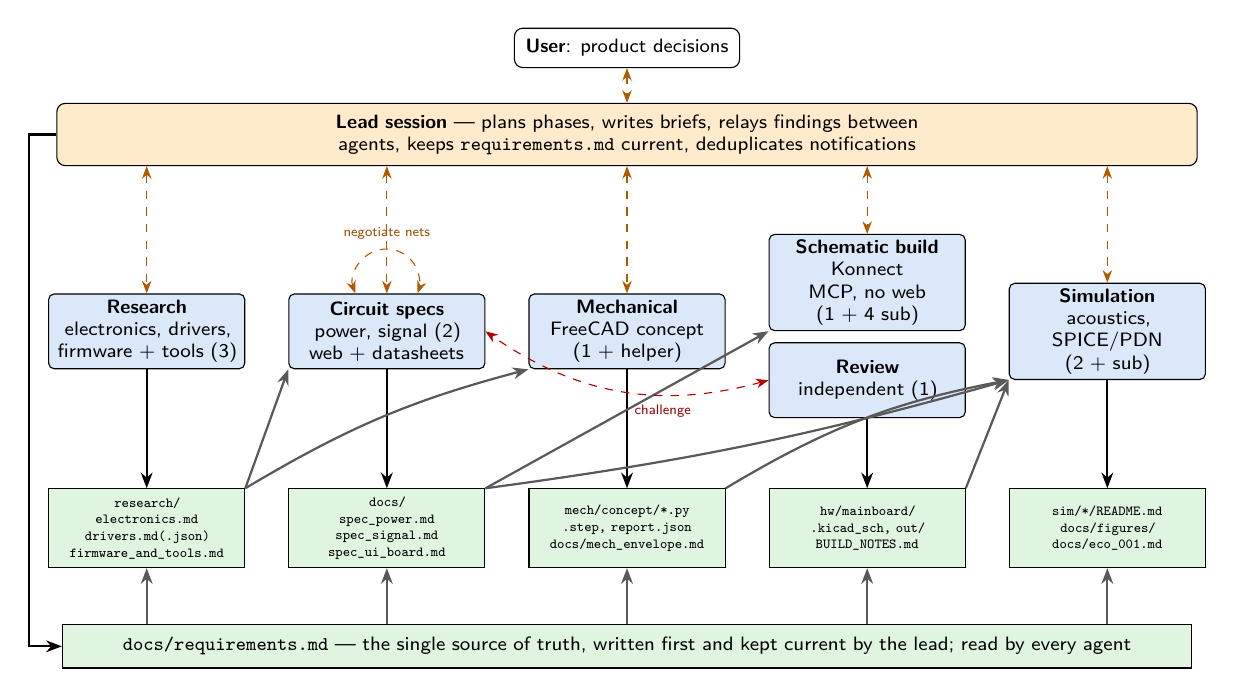
\begin{tikzpicture}[
  font=\sffamily\scriptsize,
  agent/.style={draw, rounded corners=2pt, fill=agentblue, text width=2.35cm, align=center, minimum height=0.95cm, inner sep=2pt},
  file/.style={draw, fill=filegreen, text width=2.35cm, align=center, minimum height=1.0cm, inner sep=2pt, font=\ttfamily\tiny},
  lead/.style={draw, rounded corners=3pt, fill=leadorange, align=center, inner sep=4pt},
  wr/.style={-{Stealth[length=2mm]}, thick},
  rd/.style={-{Stealth[length=2mm]}, thick, gray!70!black},
  msg/.style={{Stealth[length=1.6mm]}-{Stealth[length=1.6mm]}, dashed, orange!70!black},
]
% columns
\def\dx{3.05}
\node[agent] (res) at (0,0) {\textbf{Research}\\electronics, drivers,\\firmware + tools (3)};
\node[agent] (spec) at (\dx,0) {\textbf{Circuit specs}\\power, signal (2)\\web + datasheets};
\node[agent] (mech) at (2*\dx,0) {\textbf{Mechanical}\\FreeCAD concept\\(1 + helper)};
\node[agent] (sch) at (3*\dx,0.62) {\textbf{Schematic build}\\Konnect MCP, no web\\(1 + 4 sub)};
\node[agent] (rev) at (3*\dx,-0.62) {\textbf{Review}\\independent (1)};
\node[agent] (sim) at (4*\dx,0) {\textbf{Simulation}\\acoustics, SPICE/PDN\\(2 + sub)};

\node[file] (fres) at (0,-2.5) {research/\\electronics.md\\drivers.md(.json)\\firmware\_and\_tools.md};
\node[file] (fspec) at (\dx,-2.5) {docs/\\spec\_power.md\\spec\_signal.md\\spec\_ui\_board.md};
\node[file] (fmech) at (2*\dx,-2.5) {mech/concept/*.py\\*.step, report.json\\docs/mech\_envelope.md};
\node[file] (fsch) at (3*\dx,-2.5) {hw/mainboard/\\*.kicad\_sch, out/\\BUILD\_NOTES.md};
\node[file] (fsim) at (4*\dx,-2.5) {sim/*/README.md\\docs/figures/\\docs/eco\_001.md};

\node[file, text width=14.2cm, minimum height=0.55cm, font=\ttfamily\scriptsize] (req) at (2*\dx,-4.0)
  {docs/requirements.md \textrm{\sffamily --- the single source of truth, written first and kept current by the lead; read by every agent}};

% writes
\foreach \a/\f in {res/fres, spec/fspec, mech/fmech, sim/fsim} \draw[wr] (\a) -- (\f);
\draw[wr] (rev.south) -- (fsch.north);
% reads (next stage)
\draw[rd] (fres.north east) -- (spec.south west);
\draw[rd] (fres.north east) to[bend left=8] (mech.south west);
\draw[rd] (fspec.north east) -- (sch.south west);
\draw[rd] (fspec.north east) to[bend right=4] (sim.south west);
\draw[rd] (fmech.north east) to[bend left=10] (sim.south west);
\draw[rd] (fsch.north east) -- (sim.south west);
% review challenge
\draw[msg, red!70!black] (rev.west) to[bend left=25] node[below, font=\sffamily\tiny, text=red!60!black, pos=0.35]{challenge} (spec.east);
% spec agents talk directly
\draw[msg] (spec.north) ++(-0.4,0) arc[start angle=200, end angle=-20, radius=0.42];
\node[font=\sffamily\tiny, orange!60!black] at (\dx,1.25) {negotiate nets};
% lead and human
\node[lead, text width=14.2cm] (lead) at (2*\dx,2.5) {\textbf{Lead session} --- plans phases, writes briefs, relays findings between agents, keeps \texttt{requirements.md} current, deduplicates notifications};
\node[lead, fill=white] (user) at (2*\dx,3.6) {\textbf{User}: product decisions};
\draw[msg] (user) -- (lead);
\foreach \a in {res, spec, mech, sim} \draw[msg] (lead.south -| \a) -- (\a.north);
\draw[msg] (lead.south -| sch) -- (sch.north);
\draw[wr] (lead.west) -- ++(-0.35,0) |- (req.west);
\foreach \f in {fres, fspec, fmech, fsch, fsim} \draw[rd] (req.north -| \f) -- (\f.south);
\end{tikzpicture}
\caption{The agent workflow. Blue boxes are agents, green boxes the files they wrote. Black arrows mean ``writes'', grey arrows ``reads'', and dashed orange lines are messages through the lead. Each stage worked only from the files of earlier stages; the requirements file at the bottom is the one document every agent read.}
\label{fig:workflow}
\end{figure}

\subsection{Timeline}

Everything in \cref{tab:timeline} happened on 2026-11-24.

\begin{table}[htbp]
\centering\small
\caption{Design phases, condensed from \protect\src{docs/process_log.md}, the build notes and the reviews.}
\label{tab:timeline}
\begin{tabularx}{\linewidth}{@{}>{\raggedright\arraybackslash}p{2.9cm}>{\raggedright\arraybackslash}X@{}}
\toprule
Phase & What happened \\
\midrule
Idea, requirements & User and lead agree the concept; the lead writes \texttt{requirements.md} before any agent runs. \\
Parallel research & Three agents: parts with live JLC stock; drivers with a first-pass PR alignment; firmware/DSP plus the simulation toolchain on macOS arm64. \\
Cross-agent corrections & Firmware finds BT + Wi-Fi needs PSRAM (WROOM $\to$ WROVER); electronics finds \qty{4}{\ohm} woofers can trip the amp current limit. \\
The \qty{4}{\ohm}/\qty{8}{\ohm} flip-flop & Three contradictory relays arrive out of order; the driver agent builds, reverts and rebuilds. Set B8 (\qty{8}{\ohm}) wins. \\
Circuit specs & Two spec agents with web access write pin-exact specs and negotiate interfaces directly; they catch most of the engineering problems (\cref{sec:decisions}). \\
Mechanical concept & A scripted FreeCAD model fixes Ø\qty{95}{\milli\metre}, \qty{0.85}{\litre} and the battery; the tweeter waveguide shrinks to a bezel. \\
Schematic v0.1 & 9 sheets drawn through the Konnect MCP server: 257 parts, ERC 0, independent review without blockers. \\
Redraw & ``These schematics look awful.'' A pilot was asked for, but the agent had already redrawn every sheet with four sub-agents; a netlist comparison proved nothing changed. \\
Simulations & Acoustics (lumped, BEM, FEM, crossover) and SPICE/PDN. SPICE finds the soft amplifier rail $\to$ ECO-001. \\
Operations & Parallel sims fill the disk and RAM; a 5-hour usage limit stops all agents; work resumes from files. \\
Release review $\to$ v0.2 & Skill-driven review: no blockers, 11 should-fix items $\to$ ECO-002 and specs v1.2. A delta review of v0.2 adds two more (N1, N2) $\to$ spec v1.3. \\
\bottomrule
\end{tabularx}
\end{table}

\subsection{Verification gates}\label{sec:gates}

The schematic passed four gates before placement (\cref{fig:gates}). The release review is the one worth copying. It worked through a 44-item checklist on a hashed snapshot and traced eleven \emph{boundary states} on the netlist: blank firmware, pack insertion, ship mode, a PVDD short, and so on. Its three most important findings (S1--S3 in \cref{app:register}) were all \emph{consistent with the spec}, so ERC and the first review could not have caught them:
\begin{itemize}
  \item the short-circuit protection that depended on firmware;
  \item an unbounded inrush at pack insertion;
  \item a register default copied from a sibling chip.
\end{itemize}

\begin{figure}[htbp]
\centering
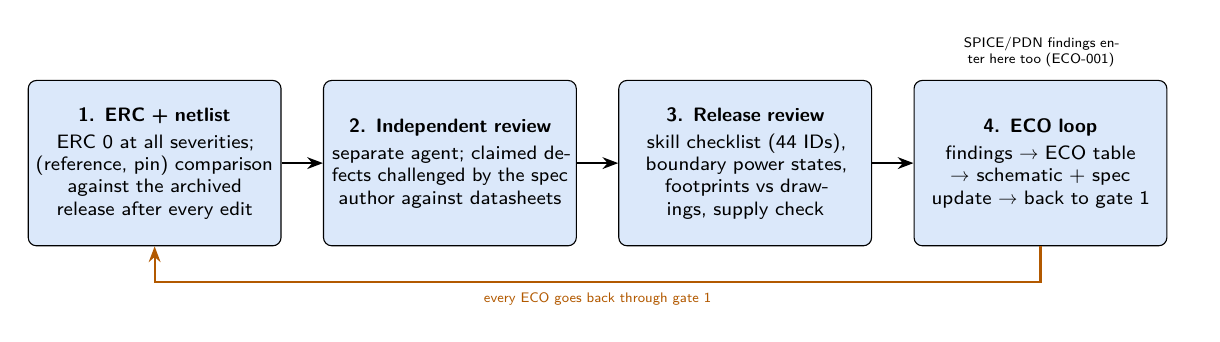
\begin{tikzpicture}[
  font=\sffamily\scriptsize,
  gate/.style={draw, rounded corners=3pt, fill=agentblue, text width=3.0cm, align=center, minimum height=2.1cm, inner sep=3pt},
  arr/.style={-{Stealth[length=2mm]}, thick},
]
\node[gate] (g1) at (0,0) {\textbf{1. ERC + netlist}\\[2pt]ERC 0 at all severities; (reference, pin) comparison against the archived release after every edit};
\node[gate] (g2) at (3.75,0) {\textbf{2. Independent review}\\[2pt]separate agent; claimed defects challenged by the spec author against datasheets};
\node[gate] (g3) at (7.5,0) {\textbf{3. Release review}\\[2pt]skill checklist (44 IDs), boundary power states, footprints vs drawings, supply check};
\node[gate] (g4) at (11.25,0) {\textbf{4. ECO loop}\\[2pt]findings $\to$ ECO table $\to$ schematic + spec update $\to$ back to gate 1};
\draw[arr] (g1) -- (g2);
\draw[arr] (g2) -- (g3);
\draw[arr] (g3) -- (g4);
\draw[arr, orange!70!black] (g4.south) -- ++(0,-0.45) -| node[pos=0.25, below, font=\sffamily\tiny]{every ECO goes back through gate 1} (g1.south);
\node[font=\sffamily\tiny, text width=3.6cm, align=center, above=1pt of g4] {SPICE/PDN findings enter here too (ECO-001)};
\end{tikzpicture}
\caption{Verification gates between ``schematic drawn'' and ``placement may start''. Each gate catches what the previous one cannot see: drawing errors, misread specs, corners the spec never considered. The ECO loop sends every change back through gate 1.}
\label{fig:gates}
\end{figure}

\subsection{What worked and what went wrong}

\begin{description}[style=nextline,leftmargin=1.2em,itemsep=3pt]
  \item[Worked] One requirements file, with specs as the contract: when the usage limit stopped every agent, nothing was lost. Spec agents with web access writing for a drawing agent without it. Independent review, followed by a challenge of each claimed defect against the datasheet. A netlist comparison after every cosmetic edit. Every simulation checked against an analytic case before use.
  \item[Went wrong] Corrections arriving out of order (\qty{4}{\ohm}/\qty{8}{\ohm}). A ``pilot first'' instruction arriving after the work had started (the redraw). Parallel heavy simulations exhausting disk and RAM. MCP tools loaded mid-session that were invisible to the agent that loaded them. Duplicate notifications, and late decisions that did not reach every file.
\end{description}

\subsection{A playbook for designing hardware with LLM agents}\label{sec:playbook}

\begin{enumerate}[label=\textbf{R\arabic*.},leftmargin=2.4em,itemsep=1pt]
  \item \textbf{Write the requirements file first and keep it current;} mark each line decided or open.
  \item \textbf{Files are the interface, messages are pointers} (``read spec\_power §4.1'', not a paraphrase).
  \item \textbf{One owner and a version per decision;} never send a correction before the last one is acknowledged.
  \item \textbf{Put pilots and stop points in the first brief,} not after the work has started.
  \item \textbf{Separate research from drawing,} and ask every spec for a ``changes vs.\ the brief'' section.
  \item \textbf{Review independently, then challenge the review} against datasheets.
  \item \textbf{Archive before cosmetic edits and verify by netlist,} not by looking at pictures.
  \item \textbf{Validate each simulation against an analytic case} and record the error.
  \item \textbf{Review boundary states,} not just the drawing: blank firmware, insertion, shorts.
  \item \textbf{End simulations and reviews in an ECO table} with severity, evidence and status.
  \item \textbf{Schedule compute like a shared lab:} one heavy job at a time, and watch the disk.
  \item \textbf{Assume interruption:} everything needed to resume must be on disk.
  \item \textbf{Fix coordinates and units in one document,} so CAD, BEM and FEM agree.
  \item \textbf{Ask agents to tag facts as measured or estimated.}
  \item \textbf{Start fresh agents after changing their tools.}
\end{enumerate}

\section{System architecture}\label{sec:architecture}

\Cref{fig:power-path,fig:data-path} show the main board as built in schematic v0.2. Power and signals are drawn separately because they share almost no parts. The schematic's own root sheet is the same block diagram drawn in KiCad (\cref{fig:sch-root}). Values are from the circuit specs, v1.2 \src{docs/spec_power.md} \src{docs/spec_signal.md}.

\begin{figure}[htbp]
\centering
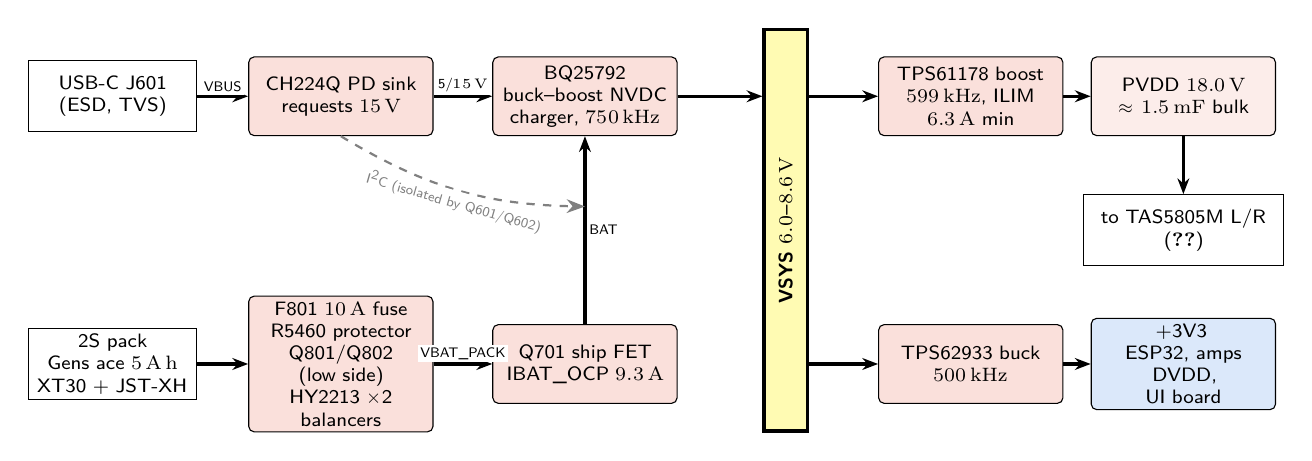
\begin{tikzpicture}[
  font=\sffamily\scriptsize,
  blk/.style={draw, fill=pwrred, rounded corners=2pt, align=center, minimum height=1.0cm, text width=2.2cm, inner sep=2pt},
  ext/.style={draw, fill=white, align=center, minimum height=0.9cm, text width=2.0cm, inner sep=2pt},
  rail/.style={-{Stealth[length=2mm]}, very thick},
  lab/.style={font=\sffamily\tiny, fill=white, inner sep=1pt},
]
\node[ext] (usb) at (0,0) {USB-C J601\\(ESD, TVS)};
\node[blk] (pd) at (2.9,0) {CH224Q PD sink\\requests \qty{15}{\volt}};
\node[blk] (chg) at (6.0,0) {BQ25792\\buck--boost NVDC\\charger, \qty{750}{\kilo\hertz}};
\node[draw, very thick, fill=yellow!30, minimum width=0.55cm, minimum height=5.1cm, align=center] (vsys) at (8.55,-1.7) {};
\node[rotate=90, font=\sffamily\scriptsize\bfseries] at (vsys) {VSYS \qtyrange{6.0}{8.6}{\volt}};
\node[blk] (boost) at (10.9,0) {TPS61178 boost\\\qty{599}{\kilo\hertz}, ILIM \qty{6.3}{\ampere} min};
\node[blk, fill=pwrred!60] (pvdd) at (13.6,0) {PVDD \qty{18.0}{\volt}\\$\approx\qty{1.5}{\milli\farad}$ bulk};
\node[blk] (buck) at (10.9,-3.4) {TPS62933 buck\\\qty{500}{\kilo\hertz}};
\node[blk, fill=digblue] (v33) at (13.6,-3.4) {+3V3\\ESP32, amps DVDD,\\UI board};
\node[ext] (pack) at (0,-3.4) {2S pack\\Gens ace \qty{5}{\ampere\hour}\\XT30 + JST-XH};
\node[blk] (prot) at (2.9,-3.4) {F801 \qty{10}{\ampere} fuse\\R5460 protector\\Q801/Q802 (low side)\\HY2213 $\times$2 balancers};
\node[blk] (ship) at (6.0,-3.4) {Q701 ship FET\\IBAT\_OCP \qty{9.3}{\ampere}};
\node[ext, text width=2.4cm] (amps) at (13.6,-1.7) {to TAS5805M L/R\\(\cref{fig:data-path})};

\draw[rail] (usb) -- node[lab, above]{VBUS} (pd);
\draw[rail] (pd) -- node[lab, above]{5/\qty{15}{\volt}} (chg);
\draw[rail] (chg.east) -- (chg.east -| vsys.west);
\draw[rail] (pack) -- (prot);
\draw[rail] (prot) -- node[lab, above]{VBAT\_PACK} (ship);
\draw[rail] (ship.north) -- node[lab, right]{BAT} (chg.south);
\draw[rail] (vsys.east |- boost.west) -- (boost);
\draw[rail] (boost) -- (pvdd);
\draw[rail] (vsys.east |- buck.west) -- (buck);
\draw[rail] (buck) -- (v33);
\draw[rail] (pvdd) -- (amps);
\draw[-{Stealth}, dashed, thick, gray] (pd.south) to[bend right=15] node[lab, pos=0.5, below, sloped]{I\textsuperscript{2}C (isolated by Q601/Q602)} (6.0,-1.4);
\end{tikzpicture}
\caption{Power path. USB-C power delivery feeds a buck--boost charger with a power-path (NVDC) output, VSYS. Everything, including the boost converter, hangs off VSYS, so the charger's \qty{6}{\ampere}-RMS battery FET and its \qty{9.3}{\ampere} over-current trip limit what the amplifiers may draw. Pack protection and cell balancing sit on the main board because the pack has none. Cell negative is not board ground: the protection FETs sit between them. There is no load-disconnect FET after the boost (\cref{sec:disconnect}), so PVDD rests at VSYS$-\qty{0.5}{\volt}$ when the boost is off.}
\label{fig:power-path}
\end{figure}

\begin{figure}[htbp]
\centering
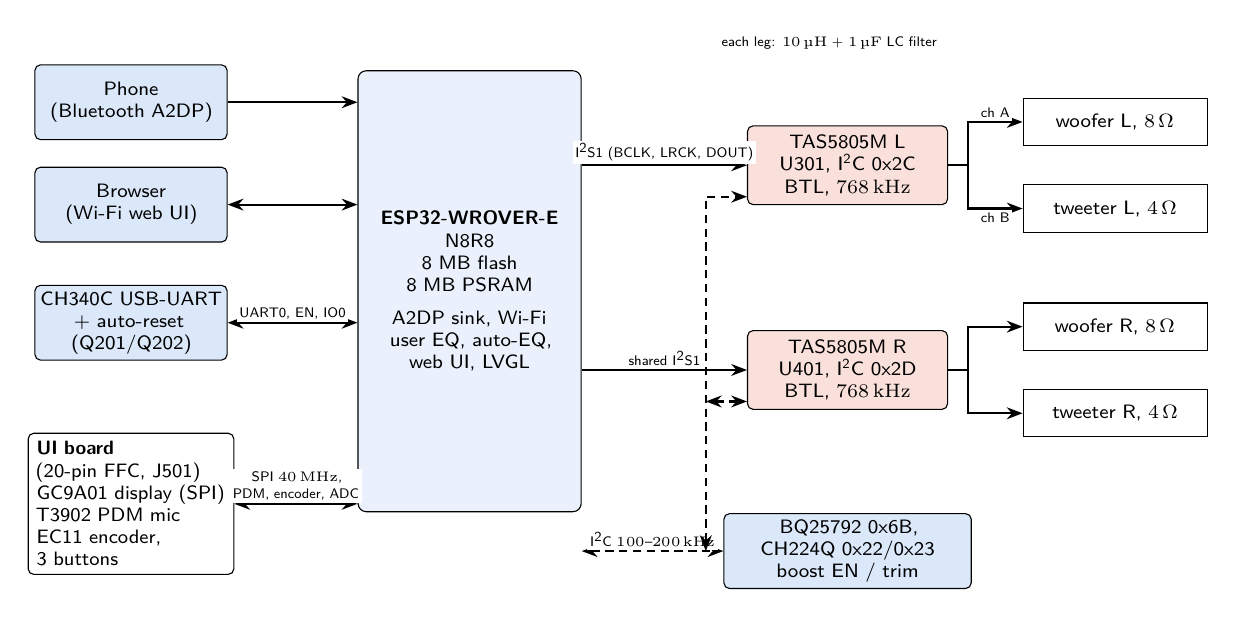
\begin{tikzpicture}[
  font=\sffamily\scriptsize,
  blk/.style={draw, fill=digblue, rounded corners=2pt, align=center, minimum height=0.95cm, text width=2.3cm, inner sep=2pt},
  amp/.style={draw, fill=pwrred, rounded corners=2pt, align=center, minimum height=1.0cm, text width=2.4cm, inner sep=2pt},
  drv/.style={draw, fill=white, align=center, minimum height=0.6cm, text width=2.2cm, inner sep=2pt},
  bus/.style={-{Stealth[length=2mm]}, thick},
  bbus/.style={{Stealth[length=2mm]}-{Stealth[length=2mm]}, thick},
  lab/.style={font=\sffamily\tiny, fill=white, inner sep=1pt},
]
\node[draw, fill=digblue!60, rounded corners=3pt, minimum height=5.6cm, text width=2.6cm, align=center] (esp) at (5.2,0) {\textbf{ESP32-WROVER-E}\\N8R8\\8 MB flash\\8 MB PSRAM\\[4pt]A2DP sink, Wi-Fi\\user EQ, auto-EQ,\\web UI, LVGL};
\node[blk] (phone) at (0.9,2.4) {Phone\\(Bluetooth A2DP)};
\node[blk] (wifi) at (0.9,1.1) {Browser\\(Wi-Fi web UI)};
\node[blk] (uart) at (0.9,-0.4) {CH340C USB-UART\\+ auto-reset (Q201/Q202)};
\node[draw, fill=white, rounded corners=2pt, text width=2.4cm, align=left, inner sep=3pt] (ui) at (0.9,-2.7) {\textbf{UI board}\\(20-pin FFC, J501)\\GC9A01 display (SPI)\\T3902 PDM mic\\EC11 encoder,\\3 buttons};
\node[amp] (ampl) at (10.0,1.6) {TAS5805M L\\U301, I\textsuperscript{2}C 0x2C\\BTL, \qty{768}{\kilo\hertz}};
\node[amp] (ampr) at (10.0,-1.0) {TAS5805M R\\U401, I\textsuperscript{2}C 0x2D\\BTL, \qty{768}{\kilo\hertz}};
\node[drv] (wl) at (13.4,2.15) {woofer L, \qty{8}{\ohm}};
\node[drv] (tl) at (13.4,1.05) {tweeter L, \qty{4}{\ohm}};
\node[drv] (wr) at (13.4,-0.45) {woofer R, \qty{8}{\ohm}};
\node[drv] (tr) at (13.4,-1.55) {tweeter R, \qty{4}{\ohm}};
\node[blk, text width=3.0cm] (pwr) at (10.0,-3.3) {BQ25792 0x6B, CH224Q 0x22/0x23\\boost EN / trim};

\draw[bus] (phone.east) -- (esp.west |- phone.east);
\draw[bbus] (wifi.east) -- (esp.west |- wifi.east);
\draw[bbus] (uart.east) -- node[lab,above]{UART0, EN, IO0} (esp.west |- uart.east);
\draw[bbus] (ui.east) -- node[lab,above, text width=1.6cm, align=center]{SPI \qty{40}{\mega\hertz}, PDM, encoder, ADC} (esp.west |- ui.east);
\draw[bus] (esp.east |- ampl.west) -- node[lab, above]{I\textsuperscript{2}S1 (BCLK, LRCK, DOUT)} (ampl.west);
\draw[bus] (esp.east |- ampr.west) -- node[lab, above]{shared I\textsuperscript{2}S1} (ampr.west);
\draw[bbus, densely dashed] (esp.east |- pwr.west) -- node[lab, above]{I\textsuperscript{2}C \qtyrange{100}{200}{\kilo\hertz}} (pwr.west);
\draw[bbus, densely dashed] (8.2,-3.3) -- (8.2,1.2) -- (ampl.south west |- 0,1.2);
\draw[bbus, densely dashed] (8.2,-1.4) -- (ampr.west |- 0,-1.4);
\draw[bus] (ampl.east) -- ++(0.25,0) |- node[lab, pos=0.75, above]{ch A} (wl.west);
\draw[bus] (ampl.east) -- ++(0.25,0) |- node[lab, pos=0.75, below]{ch B} (tl.west);
\draw[bus] (ampr.east) -- ++(0.25,0) |- (wr.west);
\draw[bus] (ampr.east) -- ++(0.25,0) |- (tr.west);
\node[font=\sffamily\tiny, text width=4.4cm, align=left] at (10.6,3.15) {each leg: \qty{10}{\micro\henry} + \qty{1}{\micro\farad} LC filter};
\end{tikzpicture}
\caption{Signal and control path. The ESP32 decodes Bluetooth audio and sends one I\textsuperscript{2}S stream to both amplifiers. Each amplifier serves one side: channel A drives the woofer and channel B the tweeter, with the crossover in the amplifier's DSP. Five devices share one I\textsuperscript{2}C bus. The PD controller is isolated from the bus when USB is unplugged (\cref{sec:ch224q}). The UI board hangs off a \qty{1.0}{\milli\metre}-pitch, 20-way flat cable that carries SPI, PDM, encoder and button signals with ground between the fast lines.}
\label{fig:data-path}
\end{figure}

\subsection{DSP split}

The DSP is split so that anything that protects hardware runs in the amplifiers, where it survives an MCU crash, and anything the user touches runs on the ESP32, where it can change smoothly \src{docs/requirements.md} \src{research/firmware_and_tools.md}.

\begin{table}[htbp]
\centering\small
\caption{Where each DSP function runs. The amplifier layer is written at boot and rarely changed. The ESP32 layer interpolates its parameters per audio block.}
\label{tab:dsp-split}
\begin{tabularx}{\linewidth}{@{}>{\raggedright\arraybackslash}X>{\raggedright\arraybackslash}X@{}}
\toprule
TAS5805M (each amplifier, 15 biquads per channel) & ESP32 (core 1 audio task, 256-frame blocks) \\
\midrule
LR4 crossover at \qty{2.5}{\kilo\hertz} (ch A low-pass, ch B high-pass) & SBC decode (AAC as a stretch goal, ESP-IDF $\ge$ 6.1) \\
Driver EQ, including the 4-biquad bass EQ from A1 and a $\approx\qty{+2}{\decibel}$ tweeter shelf (ECO-001 \#5) & User EQ and presets from the web UI and encoder \\
DRC/limiters: woofer $\le \qty{15.5}{\volt}$ peak, tweeter $\le \qty{8}{\volt}$ peak (mandatory) & Loudness, bass enhancement, stereo widening \\
Click-free volume ramps (used for mutes during coefficient changes) & Microphone auto-EQ (placement shelf) and ambient loudness \\
Process flow 1 (internal SRC to \qty{96}{\kilo\hertz}), so 44.1 and \qty{48}{\kilo\hertz} streams share one coefficient set & Digital volume mapped to AVRCP absolute volume \\
\bottomrule
\end{tabularx}
\end{table}

The firmware research estimates the whole ESP32 chain (10-band EQ, loudness, bass enhancer, widener, limiter) at about 40~Mcycle/s, roughly \qty{17}{\percent} of one \qty{240}{\mega\hertz} core, from the esp-dsp figure of 17 cycles per biquad sample \src{research/firmware_and_tools.md}. That is an estimate, not a measurement.

\subsection{GPIO and I\texorpdfstring{\textsuperscript{2}}{2}C maps}

The WROVER-E's PSRAM takes GPIO16 and GPIO17. That leaves 22 usable GPIO plus GPIO0, and \textbf{all of them are assigned} (\cref{tab:gpio}). JTAG is unavailable because GPIO12--15 are in use, so debugging goes over UART0.

{\small
\begin{longtable}{@{}r l l >{\raggedright\arraybackslash}p{0.42\linewidth}@{}}
\caption{ESP32 GPIO map, condensed from \protect\src{docs/spec_signal.md} §1.3. ``Strap'' pins are sampled at reset; the simulated strap levels are in \cref{sec:s5}.}\label{tab:gpio}\\
\toprule
GPIO & Signal & Peripheral & Notes \\
\midrule
\endfirsthead
\toprule GPIO & Signal & Peripheral & Notes \\ \midrule
\endhead
\bottomrule
\endfoot
0 & BOOT button / status LED & GPIO & Strap: 1 = SPI boot; firmware drives it open-drain only \\
1, 3 & U0TXD, U0RXD & UART0 & To CH340C \\
2 & BOOST\_EN & GPIO & Strap: must be 0 with IO0 = 0; \qty{100}{\kilo\ohm} pull-down \\
4 & ENC\_SW & GPIO / RTC wake & Moved here from GPIO36 (erratum, \cref{sec:smaller-catches}) \\
5 & LCD\_CS & VSPI CS0 & Strap, high at boot \\
12 & AMP\_PDN & GPIO & Strap MTDI: must be 0 at reset \\
13, 26, 27 & I2S\_DOUT, BCLK, LRCK & I\textsuperscript{2}S1 TX & To both amplifiers; BCLK = 64$\cdot f_s$ \\
14 & LCD\_BL & LEDC PWM & Short PWM burst during ROM boot \\
15 & LCD\_DC & GPIO & Strap MTDO \\
18, 23 & LCD\_SCLK, LCD\_MOSI & VSPI & Up to \qty{40}{\mega\hertz} over the FFC \\
19 & CHG\_INT & GPIO IRQ & BQ25792 /INT, \qty{10}{\kilo\ohm} pull-up \\
21, 22 & I2C\_SDA, I2C\_SCL & I\textsuperscript{2}C0 & \qtyrange{100}{200}{\kilo\hertz} until $t_r$ is scoped; \qty{2.2}{\kilo\ohm} pull-ups \\
25 & PVDD\_TRIM & DAC1 or LEDC & Hi-Z at reset gives PVDD = \qty{18.0}{\volt} \\
32, 33 & PDM\_CLK, PDM\_DATA & I\textsuperscript{2}S0 PDM RX & PDM RX exists only on I\textsuperscript{2}S0 \\
34, 35 & ENC\_A, ENC\_B & PCNT & Input-only \\
36 & AMP\_FAULT (1 = fault) & GPIO IRQ & Input-only; merged fault (\cref{sec:adr-fault}) \\
39 & BTN\_ADC & ADC1\_CH3 & ADC1 works with Wi-Fi on (ADC2 does not) \\
16, 17 & --- & PSRAM & Never use \\
\end{longtable}
}

\begin{table}[htbp]
\centering\small
\caption{I\textsuperscript{2}C bus map (\qty{2.2}{\kilo\ohm} pull-ups R104/R105 on the MCU sheet). The spec first assumed \qty{100}{\pico\farad} and a \qty{186}{\nano\second} rise time at \qty{400}{\kilo\hertz}. The release review added the CH224Q isolator FETs' output capacitance and got \qtyrange{240}{420}{\nano\second}, so the bus runs at \qtyrange{100}{200}{\kilo\hertz} until the rise time is scoped (review S5). Sources: \protect\src{docs/spec_power.md} §1.3, \protect\src{docs/spec_signal.md} §1.5.}
\label{tab:i2c}
\begin{tabularx}{\linewidth}{@{}l l >{\raggedright\arraybackslash}X@{}}
\toprule
Device & Address & Notes \\
\midrule
TAS5805M left (U301) & 0x2C & ADR strap \qty{4.7}{\kilo\ohm}; DSP coefficients, volume, faults \\
TAS5805M right (U401) & 0x2D & ADR strap \qty{15}{\kilo\ohm} \\
BQ25792 charger (U701) & 0x6B & Charge settings, JEITA, 16-bit ADC used as the fuel gauge \\
CH224Q PD sink (U603) & 0x22 or 0x23 & The manual does not say which; firmware probes both. Reachable only while VBUS is present \\
\bottomrule
\end{tabularx}
\end{table}

\subsection{Schematic sheets}

\begin{table}[htbp]
\centering\small
\caption{The nine hierarchical sheets of the main board, with part counts at v0.2 (counted from the exported BOM; v0.1 had 257 parts, ECO-002 added C721 and 13 test points). RefDes ranges were agreed between the two spec agents before drawing started. Source: \protect\src{hw/mainboard/BUILD_NOTES.md}, \protect\src{hw/mainboard/out/speaker_main_bom.csv}.}
\label{tab:sheets}
\begin{tabular}{@{}r l r l@{}}
\toprule
Page & Sheet & Parts & Main ICs \\
\midrule
2 & usb\_power & 17 & J601 USB-C, U603 CH224Q, U601/U602 USBLC6, Q601/Q602 I\textsuperscript{2}C isolators \\
3 & charger & 39 & U701 BQ25792, Q701 ship FET \\
4 & battery & 34 & U801 R5460N212AF, U802/U803 HY2213, Q801/Q802, F801, J801--J803 \\
5 & rails & 54 & U901 TPS61178 boost (PVDD \qty{18.0}{\volt}), U951 TPS62933 buck (+3V3) \\
6 & mcu & 42 & U101 ESP32-WROVER-E, fault merge Q101/Q102 \\
7 & usb\_uart & 8 & U201 CH340C, auto-reset Q201/Q202 \\
8 & ui\_io & 17 & J501 20-pin FFC, U501 I\textsuperscript{2}S mux (DNP), J502 \\
9 & amp\_left & 32 & U301 TAS5805M (0x2C) \\
10 & amp\_right & 28 & U401 TAS5805M (0x2D) \\
\midrule
 & \textbf{Total} & \textbf{271} & \\
\bottomrule
\end{tabular}
\end{table}

\section{Design decisions and trade-offs}\label{sec:decisions}

Each decision below is a short story: one agent found a problem, and another acted on it.

\subsection{PSRAM: from WROOM-32E to WROVER-E}\label{sec:psram}

The firmware research found that Espressif's audio framework says Bluetooth and Wi-Fi ``can not coexist without PSRAM''. With both stacks running, about \qtyrange{100}{150}{\kilo\byte} of internal heap remains, while one full LVGL frame alone needs \qty{115}{\kilo\byte} \src{research/firmware_and_tools.md}. The lead switched to the ESP32-WROVER-E-N8R8 while the electronics agent was still running. At quantity 10 it was even cheaper than the WROOM (\$3.73 against \$4.04). It cost \qty{6}{\milli\metre} of module length and GPIO16/17, which left \emph{no spare GPIO} on the board \src{research/electronics.md}.

\subsection{\texorpdfstring{\qty{4}{\ohm}}{4 Ω} or \texorpdfstring{\qty{8}{\ohm}}{8 Ω} woofers, and the amplifier current limit}\label{sec:impedance}

The TAS5805M trips at \qty{5}{\ampere}. A \qty{4}{\ohm} woofer on a \qtyrange{19}{20}{\volt} rail reaches \qtyrange{4.75}{5}{\ampere} at clipping. The driver agent re-ran its alignment with the amplifier modelled as $V_\text{peak}\le\min(\qty{18}{\volt}, \qty{4.5}{\ampere}\cdot|Z|)$. Going to \qty{8}{\ohm} cost 1--\qty{3}{\decibel}: the best \qty{4}{\ohm} set was estimated at \qty{94.4}{\decibel} pink, against \qty{91.4}{\decibel} for the \qty{8}{\ohm} set B8 \src{research/drivers.md}. After the flip-flop of \cref{sec:process}, the lead chose \textbf{B8 with PVDD = \qty{18}{\volt}}. A clipped woofer then draws only \qty{2.28}{\ampere}.

\textbf{The problem then moved to the tweeter.} The \qty{4}{\ohm} OT19NC00-04 ($R_e=\qty{3.17}{\ohm}$) would draw \qty{5.2}{\ampere} at hard clipping, including ripple. The signal spec therefore made a tweeter limiter at $\le\qty{8}{\volt}$ peak mandatory \src{docs/spec_signal.md}. SPICE confirmed it independently: \qty{5.41}{\ampere} with a clipped tone, and $\le\qty{2.7}{\ampere}$ with the limiters (\cref{sec:spice}).

\subsection{The battery hunt and the Ø\texorpdfstring{\qty{95}{\milli\metre}}{95 mm} capsule}\label{sec:battery}

The user rejected spot-welded cells, so the plan became a pre-built 2S pack with protection on the board. The mechanical agent found that the geometry decided the rest \src{docs/mech_envelope.md}:
\begin{itemize}
  \item The \qty{48}{\milli\metre}-deep woofers, rear-mounted, leave only a \qtyrange{19}{23}{\milli\metre} slab behind their motors.
  \item At Ø\qty{90}{\milli\metre} that slab shrinks to about \qty{16}{\milli\metre}, which would need a pack no thicker than \qty{13}{\milli\metre}. No stocked pack was that thin with enough capacity.
\end{itemize}
The choice was a Gens ace \qty{5000}{\milli\ampere\hour} 2S RC pack: \qtyproduct{109 x 42 x 19.5}{\milli\metre}, \qty{37}{\watt\hour}, about \$31. It fits a Ø\qty{95}{\milli\metre} capsule with \qty{1}{\milli\metre} to spare and a \qty{10}{\percent} swell allowance. At a \qty{2.9}{\watt} ``moderate'' average it runs about \qty{12.8}{\hour}, against the \qty{8}{\hour} target. The pack has no protection circuit, no NTC (one is bonded on) and no published continuous rating, so it must be bench-tested at \qty{6}{\ampere}. The board's protection was designed for exactly this kind of pack.

\subsection{Removing the boost load-disconnect FET}\label{sec:disconnect}

TI's rules for the TPS61178's optional disconnect FET require the capacitance after the FET to be at most $10\times$ the capacitance before it. Here it would be about $40\times$ (\qty{1.5}{\milli\farad} against \qty{36}{\micro\farad}), and start-up would risk tripping the hiccup protection. The power-spec agent removed the FET \src{docs/spec_power.md}. PVDD now rests at VSYS$-\qty{0.5}{\volt}$ when the boost is off, with the amplifiers in shutdown drawing about \qty{30}{\micro\ampere}.

The release review later showed what the spec had assumed:
\begin{itemize}
  \item \textbf{Short protection depends on firmware.} A PVDD short is cleared only by the charger's \qty{9.3}{\ampere} battery over-current trip, which works only while firmware keeps it armed; a watchdog expiry disarms it (S1).
  \item \textbf{Inrush at pack insertion is not bounded:} \qtyrange{2.5}{9.7}{\ampere} through the ship FET (S2).
\end{itemize}
The first became the top item of the firmware contract (\cref{sec:firmware-req}). The second added a DNP gate--source footprint, C721, with a corrected fitting rule (N1, \cref{tab:firmware-req}).

\subsection{The ADR/FAULT pin}\label{sec:adr-fault}

The brief asked for one shared open-drain fault line from both amplifiers. The signal-spec agent found that the TAS5805M's pin 3 is \texttt{ADR/FAULT}: it reads the I\textsuperscript{2}C address resistor at power-up, then becomes a push-pull FAULTZ output. Tying the two pins together would have given \emph{both amplifiers the same address}. The fix keeps separate address resistors and merges the two FAULTZ signals with two 2N7002s in series. The merged AMP\_FAULT on GPIO36 is active-high, and the FETs load the address straps by only \qty{1.5}{\percent} \src{docs/spec_signal.md}.

\subsection{CH224Q back-driving the I\texorpdfstring{\textsuperscript{2}}{2}C bus}\label{sec:ch224q}

The PD controller shares the I\textsuperscript{2}C bus but is powered only from USB. Unpowered, its internal pull-ups become pull-downs and would drag the \qty{3.3}{\volt} bus to about \qty{2.2}{\volt}, below the input-high threshold. On battery the speaker would have lost control of its amplifiers. Two FETs with their gates on VBUS/2 now isolate the PD controller when USB is absent. They also set a firmware rule: never request \qty{28}{\volt} EPR, because the gates would see \qty{14}{\volt} \src{docs/spec_power.md}. The release review later found that the FETs' output capacitance may slow the bus edges, so I\textsuperscript{2}C runs at \qtyrange{100}{200}{\kilo\hertz} until the rise time is measured (S5).

\subsection{Smaller catches}\label{sec:smaller-catches}

\begin{itemize}[itemsep=1pt]
  \item The HY2213 balancers are gate drivers, not bleeders: each cell needs its own FET and resistors.
  \item ESP32 erratum: GPIO36/39 glitch when ADC1 starts, so the encoder switch moved to GPIO4.
  \item No JLC stock of JST-SH, so the UI link became a 20-pin FFC, with its own signal-integrity study (\cref{sec:spice}).
  \item Battery negative is not ground (low-side protector), so BATT\_N must be its own copper island.
  \item The charger's power-on charge current is \qty{2}{\ampere}, not the \qty{1}{\ampere} copied from its sibling chip (S3).
  \item Charging temperature is now sensed on the pack's own NTC, not on the board (ECO-002).
  \item An external power button was added through FFC pin 20. Firmware cannot see it, so it only wakes and resets; ``off'' is a long press of the encoder (N2).
\end{itemize}

\subsection{Change orders}\label{sec:eco}

The SPICE/PDN agent wrote its findings as an engineering change order rather than a report (\cref{tab:eco}) \src{docs/eco_001.md}. ECO-002 did the same for the release review; it is summarised in \cref{app:register}. Both are applied in schematic v0.2.

\begin{table}[htbp]
\centering\small
\caption{ECO-001, from the circuit simulations. Items 1--4 are applied in the schematic; 5--6 are firmware requirements.}
\label{tab:eco}
\begin{tabularx}{\linewidth}{@{}c >{\raggedright\arraybackslash}p{0.36\linewidth} >{\raggedright\arraybackslash}X@{}}
\toprule
\# & Change & Evidence \\
\midrule
1 & Boost compensation \qty{33}{\kilo\ohm}/\qty{47}{\nano\farad} $\to$ \qty{100}{\kilo\ohm}/\qty{15}{\nano\farad} & PVDD impedance \qtyrange{0.46}{0.57}{\ohm} at \qty{150}{\hertz} against a \qty{0.14}{\ohm} target; load-step dip \qty{0.97}{\volt} $\to$ \qty{0.34}{\volt} \\
2 & Fit the trim network R907/D901 for a firmware soft start & Start-up windup overshoots to \qty{19.4}{\volt} (typ.) or the \qty{21}{\volt} OVP \\
3 & SPI/PDM source resistors \qty{33}{\ohm} $\to$ \qty{68}{\ohm} & \qtyrange{0.7}{1.1}{\volt} overshoot on the FFC \\
4 & ESP32 EN capacitor \qty{1}{\micro\farad} $\to$ \qty{2.2}{\micro\farad} & Auto-reset fails if the host's DTR/RTS gap exceeds \qty{2.5}{\milli\second} \\
5 & Tweeter EQ: \qty{+2}{\decibel} high shelf (firmware) & LC filter droop \qty{-2.2}{\decibel} at \qty{20}{\kilo\hertz} \\
6 & Stop charging above \qty{45}{\degreeCelsius} (firmware) & The hardware window runs to \qty{60.8}{\degreeCelsius} \\
\bottomrule
\end{tabularx}
\end{table}

\section{Feature tour}\label{sec:features}

\subsection{Stereo two-way, bi-amplified}

Each side has its own TAS5805M in bridge-tied-load (BTL) mode \src{docs/spec_signal.md} §3:
\begin{itemize}
  \item Channel A drives the \qty{8}{\ohm} woofer and channel B the \qty{4}{\ohm} tweeter. The amplifier's input mixer sends the left (or right) input to both of its channels, and each channel's 15 biquads implement the LR4 low-pass or high-pass plus that driver's EQ.
  \item The firmware research pointed out that TI's tested topology is ``2.2 dual stereo'' (one chip for both woofers, one for both tweeters). The per-side split was kept. The research noted that TI's split would also put both woofers' current demand on a single chip \src{research/firmware_and_tools.md}.
  \item The amplifiers switch at \qty{768}{\kilo\hertz}. Each output leg has a \qty{10}{\micro\henry} inductor ($I_\text{sat}=\qty{5.5}{\ampere}$) and a \qty{1}{\micro\farad} capacitor, which places the differential filter corner at \qty{50.3}{\kilo\hertz}.
  \item The boost runs at \qty{599}{\kilo\hertz}. That keeps its low-order beats with the amplifier clock at least \qty{91}{\kilo\hertz} away from audio at nominal frequency.
  \item The analog gain is set so that 0 dBFS is about PVDD (AGAIN = 8, \qty{18.6}{\volt} peak at full scale).
\end{itemize}

Acoustically, the woofers sit only \qty{66}{\milli\metre} apart, behind Ø\qty{53}{\milli\metre} tunnels in the front baffle. The tweeters are \qty{166}{\milli\metre} apart on the front shoulders, aimed \ang{40} upward, so they carry most of the stereo image \src{docs/mech_envelope.md}. The two passive radiators on the end caps share the woofers' box and are tuned to \qty{53.2}{\hertz} with \qty{3.5}{\gram} of washers each (\cref{sec:a1}).

\subsection{Microphone auto-EQ}

A TDK T3902 bottom-port PDM microphone sits on the underside of the UI board. A gasketed printed tube connects it to a Ø\qty{1}{\milli\metre} port in the top of the shell, so it hears the room and not the inside of the box. It runs at a PDM clock of $64\cdot f_s = \qty{3.072}{\mega\hertz}$ at \qty{48}{\kilo\hertz}, inside the mic's high-quality-mode range \src{docs/spec_signal.md} \src{docs/spec_ui_board.md}. The firmware research proposes two v1 algorithms \src{research/firmware_and_tools.md}:
\begin{enumerate}
  \item \textbf{Placement (boundary) bass compensation.}
  \begin{itemize}
    \item Fade the music and play a \qty{2}{\second} log sweep (\qty{30}{\hertz} to \qty{2}{\kilo\hertz}).
    \item Deconvolve the recording, window the impulse response to about \qty{20}{\milli\second}, and compare it with a free-field reference stored in flash.
    \item Fit a single low shelf, cut-biased so boost is at most \qty{+2}{\decibel} to protect excursion.
  \end{itemize}
  The fallback is a three-way classifier (free, near a wall, corner) mapped to presets of 0, \qty{-3}{\decibel} and \qty{-6}{\decibel} at \qty{150}{\hertz}.
  \item \textbf{Ambient-adaptive loudness.} A minimum-statistics noise tracker subtracts the speaker's own predicted contribution. It raises the gain by half the noise excess above \qty{45}{\decibel}A, capped at \qty{+10}{\decibel} and slewed at no more than \qty{1}{\decibel} per \qty{3}{\second}.
\end{enumerate}
The biggest risk is structure-borne vibration reaching the microphone. The panel-mode study (\cref{sec:a4}) shows that the top of the shell, where the mic sits, has the strongest local motion below \qty{1}{\kilo\hertz}.

\subsection{Live EQ over Wi-Fi}

The ESP32 joins the home network as a station and serves a single-page web app from LittleFS. SoftAP is used only for provisioning, because ESP-IDF rates ``SoftAP + BT connected'' as unstable. User EQ runs on the ESP32 with per-block parameter interpolation, so slider moves do not click \src{research/firmware_and_tools.md}.

The amplifier biquads can also be rewritten live:
\begin{itemize}
  \item The research agent decoded the coefficient format: signed 5.27 fixed point, stored as $b_0, b_1, b_2, -a_1, -a_2$. It checked the format against a PurePath Console dump with its own encoder, \texttt{tools/tas5805m\_bq.py}.
  \item One biquad costs about \qty{0.6}{\milli\second} of I\textsuperscript{2}C at \qty{400}{\kilo\hertz}, so all 60 biquads take about \qty{40}{\milli\second}. Until the bus rise time has been measured the bus runs at \qty{100}{\kilo\hertz}--\qty{200}{\kilo\hertz} (review S5), where one biquad takes about \qty{2.4}{\milli\second} at \qty{100}{\kilo\hertz} \src{docs/spec_signal.md}.
  \item TI documents no safe-load bank, so multi-biquad changes use a mute ramp, then the writes, then an unmute ramp.
\end{itemize}

\subsection{Round display and controls}

The display is a Waveshare 1.28-inch GC9A01 module ($240\times240$) behind a lens on the top. It runs on SPI at up to \qty{40}{\mega\hertz} over the flat cable, which takes about \qty{23}{\milli\second} per full frame. LVGL redraws only small areas (level meter, rotary arc), using two \qty{11.5}{\kilo\byte} partial buffers in internal DMA-capable RAM \src{research/firmware_and_tools.md}.

The other controls are an EC11 encoder with push switch, read by the pulse counter, and three buttons on an ADC1 resistor ladder. A fourth button, SW4, is the power button. ECO-002 routes the charger's /QON input to it over J501 pin 20, with no pull-up (the charger has one inside) and a small TVS. A \qty{1}{\second} press wakes the speaker from ship mode, and a \qty{10}{\second} press resets the whole system, which is also the only battery-side reset of a hung ESP32 \src{docs/spec_ui_board.md} \src{docs/eco_002.md}.

\subsection{USB-C PD charging and flashing}

\begin{itemize}
  \item \textbf{PD request.} The CH224Q requests \qty{15}{\volt} at attach, set by a \qty{56}{\kilo\ohm} resistor on CFG1. Firmware can read the source's current capability (register 0x50) and program the charger's input current limit from it \src{docs/spec_power.md}.
  \item \textbf{Charger.} The BQ25792 is a four-switch buck--boost NVDC charger at \qty{750}{\kilo\hertz} with a \qty{2.2}{\micro\henry} inductor. It plays while charging and has a 16-bit ADC that serves as the fuel gauge.
  \item \textbf{Limits.} A hardware input-current clamp sits at \qtyrange{2.72}{2.89}{\ampere}. Firmware writes the charge current at boot, $\le\qty{2.5}{\ampere}$ (0.5C) for the \qty{5}{\ampere\hour} pack; the power-on default is \qty{2}{\ampere}. The NTC window is \qtyrange{2.0}{60.8}{\degreeCelsius} (\cref{sec:s3}), measured on the pack's own NTC by default (ECO-002 \#3).
  \item \textbf{Ship mode.} Ship mode draws about \qty{15}{\micro\ampere} from the pack, so a \qty{5}{\ampere\hour} pack lasts years on the shelf.
  \item \textbf{Flashing.} The same USB-C connector carries USB 2.0 to a CH340C with the two-transistor DTR/RTS auto-reset, so \texttt{esptool} can flash without buttons (\cref{sec:s5}).
\end{itemize}

\section{Engineering analysis}\label{sec:analysis}

Every simulation answers one design question and ends in a design decision. Each model was checked against an analytic or published case before its results were used; the checks are collected in one box per part. Everything can be rerun from \repo{sim/acoustics/run_all.sh} and \repo{sim/spice/run_all.sh}. The full write-ups are \repo{sim/acoustics/README.md} and \repo{sim/spice/README.md}.

\begin{table}[htbp]
\centering\small
\caption{The simulations at a glance.}
\label{tab:sim-summary}
\begin{tabularx}{\linewidth}{@{}l >{\raggedright\arraybackslash}p{0.33\linewidth} >{\raggedright\arraybackslash}X@{}}
\toprule
ID & Question & Outcome \\
\midrule
A1 & PR tuning, bass limits, bass EQ & \qty{3.5}{\gram} per PR, $f_b=\qty{53}{\hertz}$; $F_3$ \qty{63.7}{\hertz}; \qty{90.6}{\decibel} pink; no zeolite \\
A2 & Tweeter bezel or waveguide? & Keep the \qty{3}{\milli\metre} bezel; the desk, not the bezel, is the problem \\
A3 & Woofer baffle step, tunnel & Smooth \qty{-5.6}{\decibel} step, cancelled by the desk; keep the tunnel (+3--\qty{4}{\decibel} horn bump) \\
A4 & Panel modes of the printed shell & Output $\ge\qty{23}{\decibel}$ below the woofers; add a spine plate and damping \\
A5 & Crossover and system EQ & LR4 at \qty{2.5}{\kilo\hertz}, tweeter \qty{-9.7}{\decibel}, \qty{+110}{\micro\second}; 7-biquad EQ \\
S1/S7 & Boost loop, start-up, rail impedance & Stable but soft at \qty{150}{\hertz}; start-up windup $\to$ ECO-001 \#1, \#2 \\
S2 & Class-D filter into real drivers & Tweeter limiter mandatory; \qty{+2}{\decibel} tweeter shelf \\
S3--S5 & NTC window, PVDD trim, ESP32 reset & \qtyrange{2.0}{60.8}{\degreeCelsius}; trim settles in $\le\qty{150}{\milli\second}$; EN capacitor \qty{2.2}{\micro\farad} \\
S6 & Flat-cable signal integrity & \qty{68}{\ohm} source resistors; \qty{53}{\mega\hertz} max SPI \\
\bottomrule
\end{tabularx}
\end{table}

% =====================================================================
\subsection{Acoustics}

The acoustic results are referenced to a \emph{seated listener}: the speaker stands on a desk, and the listener's ears are \qty{1.0}{\metre} in front of it and \qty{0.40}{\metre} above the desk top, which puts them \ang{21} below the tweeter axis. A grid of 15 seats around that point gives a ``listening-window'' average \src{sim/acoustics/README.md}.

\subsubsection{A1: Bass system (lumped model)}\label{sec:a1}

A Thiele/Small model puts two ND65-8 woofers and two DMA58-PRs in one \qty{0.82}{\litre} box. The amplifier enters as limits, not as a fixed power: a \qty{15.5}{\volt} woofer limiter (about \qty{15}{\watt}) and \qty{4.5}{\ampere} of current. The maximum output at each frequency is the lowest of four limits: amplifier voltage, amplifier current, woofer $X_\text{max}$ and PR excursion.

\textbf{Result.}
\begin{itemize}
  \item With \qty{3.5}{\gram} of washers per PR, the box tunes to \qty{53.2}{\hertz}.
  \item A four-biquad bass EQ (at most \qty{+8.8}{\decibel}) gives $F_3/F_6 = \qtylist{63.7;55.3}{\hertz}$.
  \item The pink-noise maximum is \qty{90.6}{\decibel} at \qty{1}{\metre} in half space, limited by amplifier voltage. That is only \qty{0.5}{\decibel} above the target.
\end{itemize}
Because voltage is the binding limit, stuffing and zeolite each move the result by less than \qty{0.5}{\decibel}, so zeolite was dropped. The only cheap lever is the limiter: \qty{17.1}{\volt} would add \qty{0.9}{\decibel}, at the price of overdriving the woofer's \qty{15}{\watt} rating. Both the SPL and $F_6$ margins rest on vendor T/S data, so the drivers get measured first.

\begin{figure}[htbp]
\centering
\begin{subfigure}[t]{0.49\linewidth}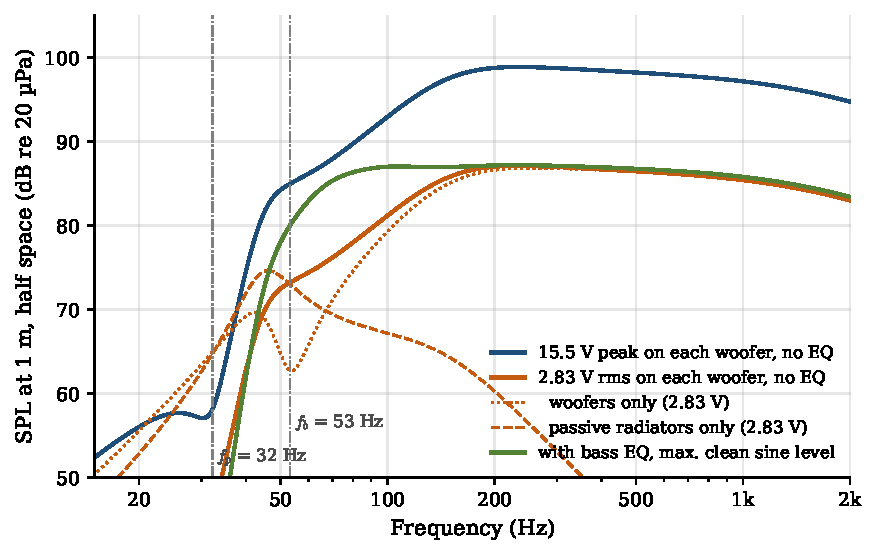
\includegraphics[width=\linewidth]{a1_spl_halfspace_1m.pdf}\caption{SPL at \qty{1}{\metre}, half space: woofer and PR contributions, full drive and the EQ'd maximum, with $f_b$ and the PR notch marked.}\end{subfigure}\hfill
\begin{subfigure}[t]{0.49\linewidth}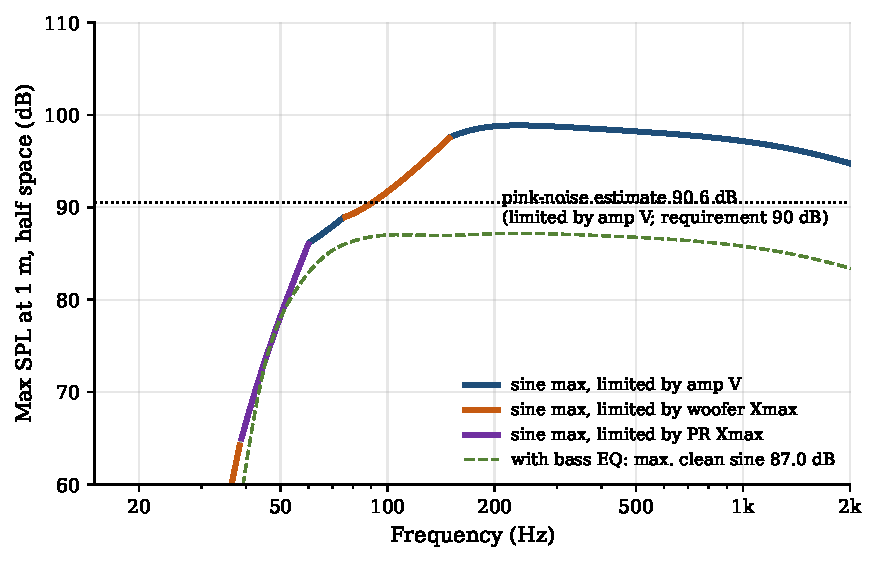
\includegraphics[width=\linewidth]{a1_max_spl_vs_frequency.pdf}\caption{Maximum sine SPL coloured by the binding limit: PR excursion below \qty{60}{\hertz}, $X_\text{max}$ from 75 to \qty{150}{\hertz}, amplifier voltage elsewhere.}\end{subfigure}\\[4pt]
\begin{subfigure}[t]{0.49\linewidth}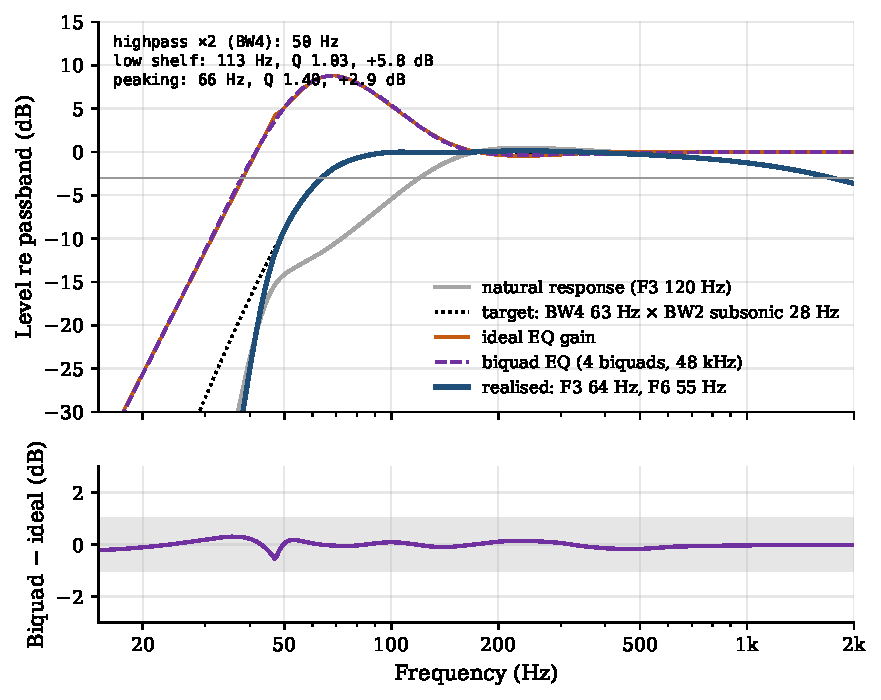
\includegraphics[width=\linewidth]{a1_dsp_bass_eq.pdf}\caption{Bass EQ: natural response, Butterworth target, 4-biquad fit (error $\le\qty{0.55}{\decibel}$).}\end{subfigure}\hfill
\begin{subfigure}[t]{0.49\linewidth}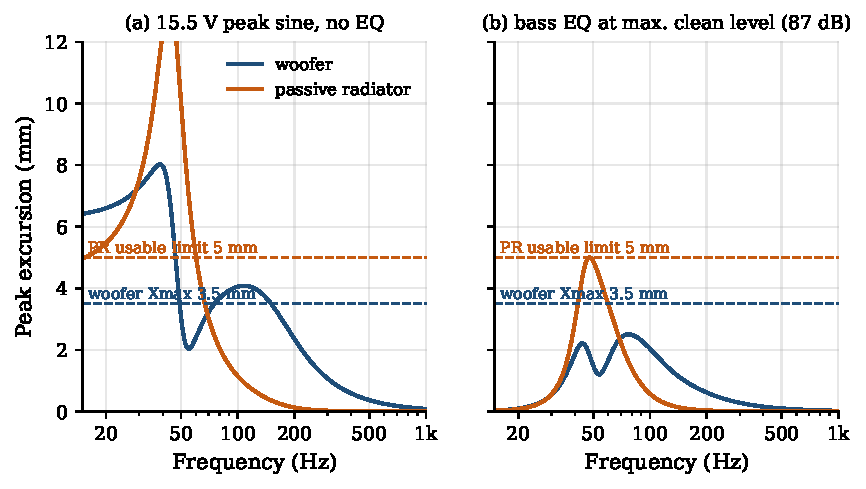
\includegraphics[width=\linewidth]{a1_excursion_vs_xmax.pdf}\caption{Excursion against limits; with EQ the PR reaches \qty{5}{\milli\metre} at \qty{48}{\hertz}, hence the subsonic roll-off.}\end{subfigure}\\[4pt]
\begin{subfigure}[t]{0.49\linewidth}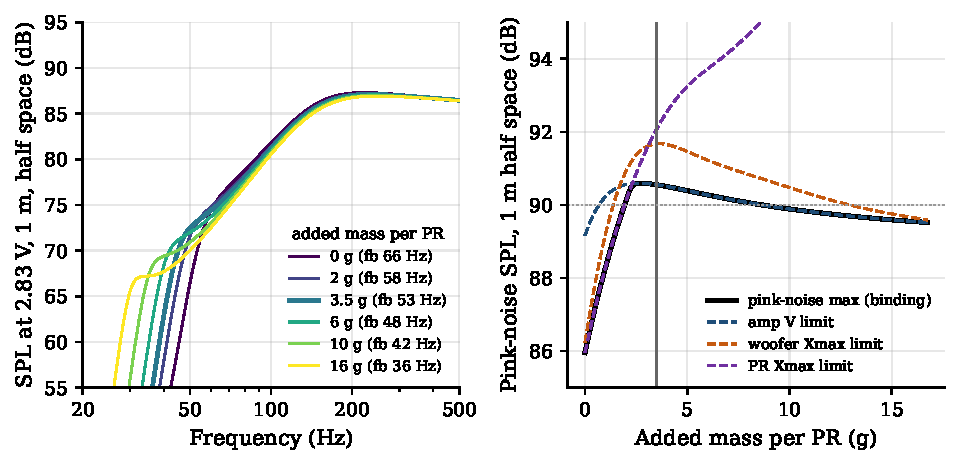
\includegraphics[width=\linewidth]{a1_pr_mass_sweep.pdf}\caption{PR mass sweep, 0--\qty{16}{\gram}: the optimum is flat from 2.5 to \qty{4}{\gram}.}\end{subfigure}\hfill
\begin{subfigure}[t]{0.49\linewidth}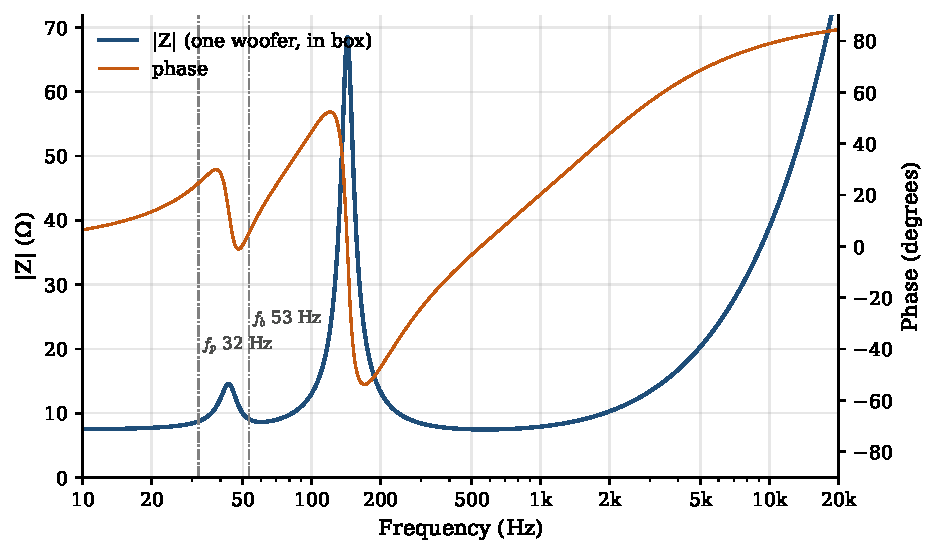
\includegraphics[width=\linewidth]{a1_impedance.pdf}\caption{Woofer impedance in the PR box: the dip near \qty{61}{\hertz} is used to tune the PRs on the bench.}\end{subfigure}
\caption{A1: the bass system. Two \qty{2.5}{inch} woofers and two passive radiators in under a litre reach \qty{64}{\hertz} with a modest DSP lift.}
\label{fig:a1}
\end{figure}

\begin{figure}[htbp]
\centering
\begin{subfigure}[t]{0.49\linewidth}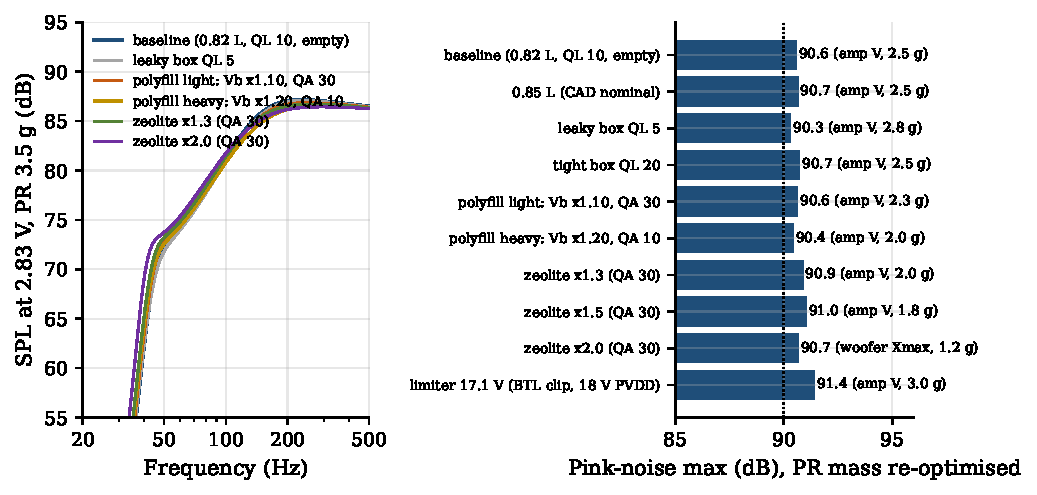
\includegraphics[width=\linewidth]{a1_whatif_volume_fill_zeolite.pdf}\caption{What-ifs: leakage, polyfill, zeolite, limiter. Only the limiter moves the pink-noise maximum by more than \qty{0.5}{\decibel}.}\end{subfigure}\hfill
\begin{subfigure}[t]{0.49\linewidth}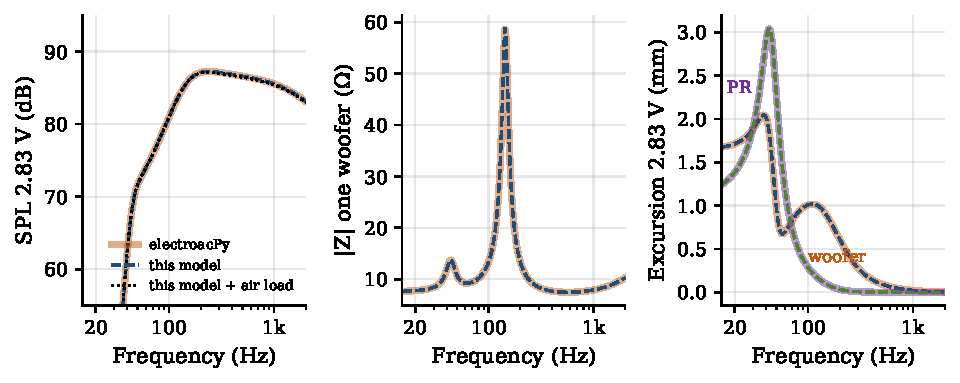
\includegraphics[width=\linewidth]{a1_electroacpy_crosscheck.pdf}\caption{Validation against electroacPy: SPL within \qty{0.013}{\decibel}, impedance within \qty{0.22}{\percent}.}\end{subfigure}\\[4pt]
\begin{subfigure}[t]{0.6\linewidth}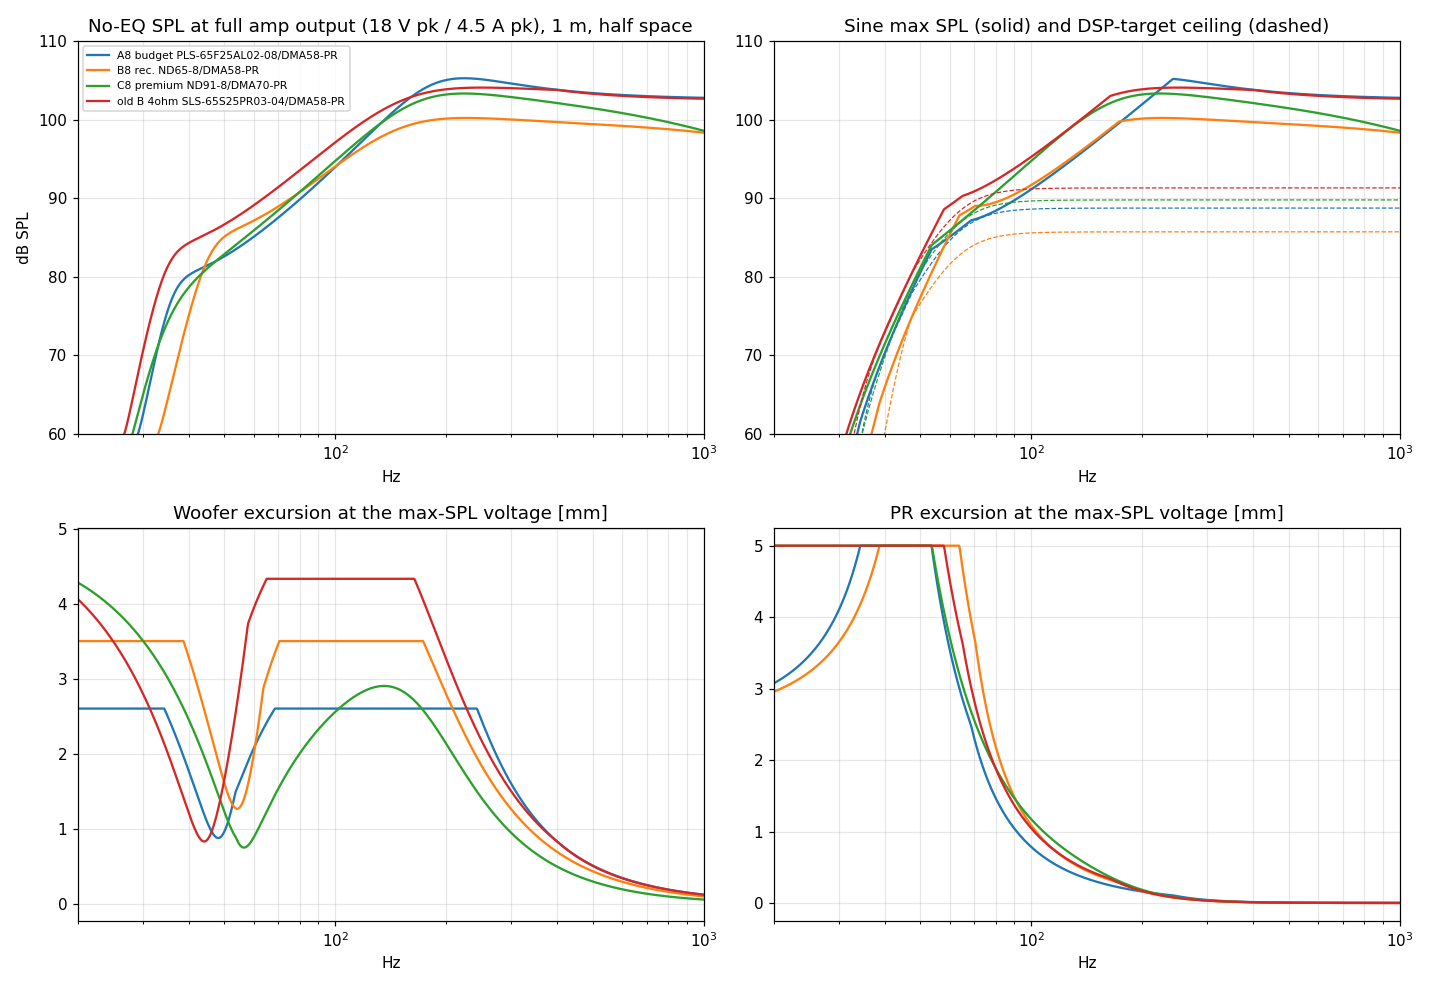
\includegraphics[width=\linewidth]{pr_alignment_firstpass.png}\caption{History: the driver agent's first-pass alignment (\qty{0.75}{\litre}, \qty{19}{\volt}), used to choose set B8.}\end{subfigure}
\caption{A1: what-ifs, validation and the first-pass model that chose the drivers.}
\label{fig:a1-more}
\end{figure}

\subsubsection{The BEM model behind A2, A3 and A5}\label{sec:bem}

The boundary-element model treats the capsule as a rigid body in free air. Each of the six radiators is a rigid piston, and bempp-cl solves the exterior problem at each of about 88 frequencies from \qty{105}{\hertz} to \qty{16}{\kilo\hertz}. Any real drive is a weighted sum of the six unit solutions. The hull is rebuilt in gmsh from the FreeCAD parameter block, so a CAD change flows straight into the acoustics. The desk is added as an image source. The meshes hold $h\le\lambda/6$, with a 9, 5.6 or \qty{3.5}{\milli\metre} global size per band and \qty{2.8}{\milli\metre} around the tweeters, giving 4\,k to 10\,k unknowns. CHIEF interior points suppress the spurious resonances of the plain formulation. The four cases run in about \qty{75}{\minute} on the laptop.

\begin{figure}[htbp]
\centering
\begin{subfigure}[t]{0.49\linewidth}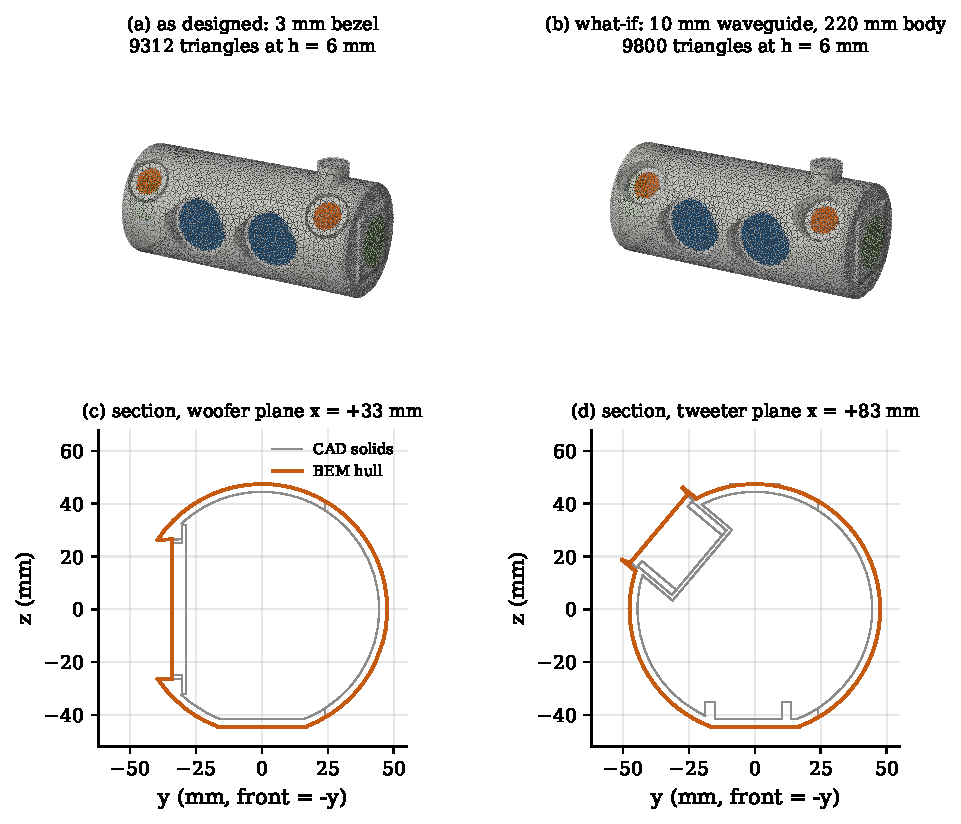
\includegraphics[width=\linewidth]{a2_a3_bem_hull_mesh_and_cad_check.pdf}\caption{Bezel and waveguide hulls with the pistons coloured, and hull sections over the CAD (median gap \qtyrange{0.7}{0.9}{\milli\metre}).}\end{subfigure}\hfill
\begin{subfigure}[t]{0.49\linewidth}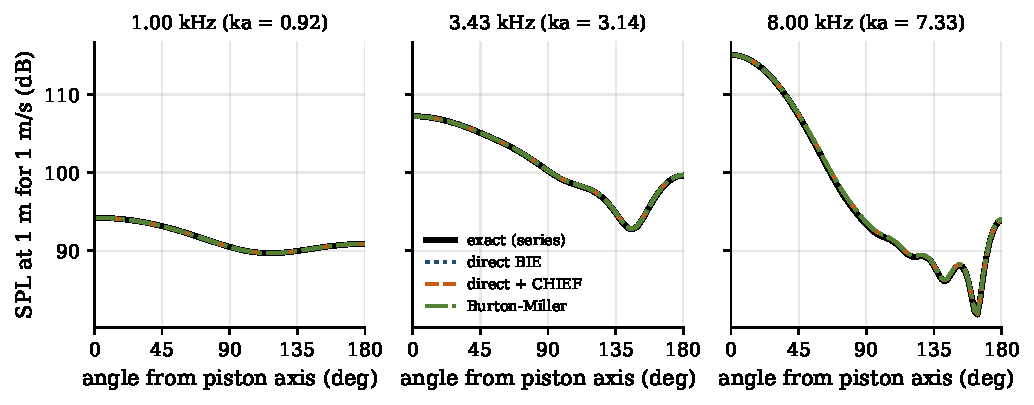
\includegraphics[width=\linewidth]{a2_a3_bem_validation_sphere_piston.pdf}\caption{Piston on a sphere against the exact solution: \qty{0.34}{\decibel} at $ka=7.3$.}\par\medskip
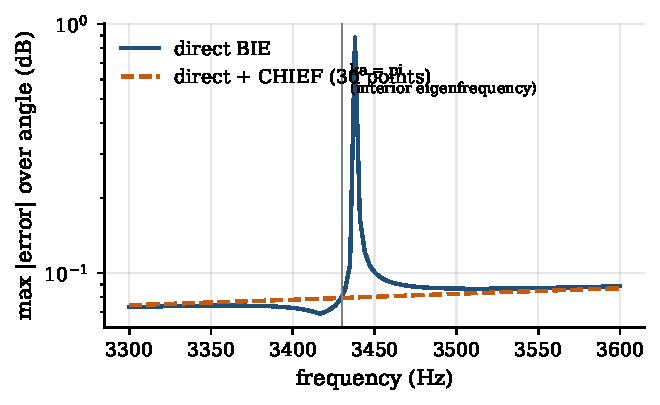
\includegraphics[width=0.8\linewidth]{a2_a3_bem_validation_irregular_frequency.pdf}\caption{Through the first interior resonance: the plain equation fails (\qty{0.88}{\decibel}); CHIEF does not.}\end{subfigure}
\caption{The BEM model and its validation.}
\label{fig:bem}
\end{figure}

\subsubsection{A2: Tweeter bezel, waveguide or flat baffle}\label{sec:a2}

\textbf{Question.} The mechanical concept had room only for a \qty{3}{\milli\metre} bezel. Would a \qty{10}{\milli\metre} waveguide, which needs a capsule about \qty{10}{\milli\metre} longer, be worth it?

\begin{table}[htbp]
\centering\small
\caption{A2: tweeter on the real capsule. Source: \protect\src{sim/acoustics/README.md}.}
\label{tab:a2}
\begin{tabular}{@{}l c c c@{}}
\toprule
 & \textbf{\qty{3}{\milli\metre} bezel} & \qty{10}{\milli\metre} waveguide & Flat baffle \\
\midrule
$-6$~dB beamwidth, horizontal, 2.5 / 5 / \qty{10}{\kilo\hertz} & \ang{310} / \ang{190} / \ang{110} & \ang{235} / \ang{128} / \ang{70} & \ang{185} \\
Directivity index, 2.5 / \qty{10}{\kilo\hertz} & 3.0 / \qty{7.9}{\decibel} & 3.8 / \qty{11.1}{\decibel} & 3.2 / \qty{6.5}{\decibel} \\
On-axis SPL, \qty{2.83}{\volt}, \qty{5}{\kilo\hertz} & \qty{87.6}{\decibel} & \qty{92.1}{\decibel} & \qty{87.3}{\decibel} \\
On-axis ripple, 2--\qty{12}{\kilo\hertz} & \textbf{\qty{2.1}{\decibel}} & \qty{4.7}{\decibel} & \qty{0.6}{\decibel} \\
Listener (\ang{21} below axis) re axis, 5 / \qty{10}{\kilo\hertz} & +0.8 / \qty{-1.8}{\decibel} & $-0.2$ / \qty{-2.6}{\decibel} & $-0.2$ / \qty{-0.8}{\decibel} \\
Desk dip, centre seat / 15-seat average & $-14.8$ / \qty{-5.6}{\decibel} & $-11.8$ / \qty{-5.3}{\decibel} & --- \\
\bottomrule
\end{tabular}
\end{table}

\textbf{Result: keep the bezel} (\cref{tab:a2}). The listener hears within \qty{2}{\decibel} of on-axis up to \qty{10}{\kilo\hertz}. The waveguide buys 3--\qty{4}{\decibel} of sensitivity, but the tweeter already runs \qty{10}{\decibel} below the woofer (A5), and this short, unoptimised flare doubles the ripple. The real treble problem is \textbf{the desk}: its reflection cancels the direct sound near \qty{2.8}{\kilo\hertz} at the centre seat (\qty{-15}{\decibel}). The dip moves with ear height, so EQ must not fill it. The physical cures are a 5--\ang{10} backward tilt on feet, or more tweeter height.

\begin{figure}[htbp]
\centering
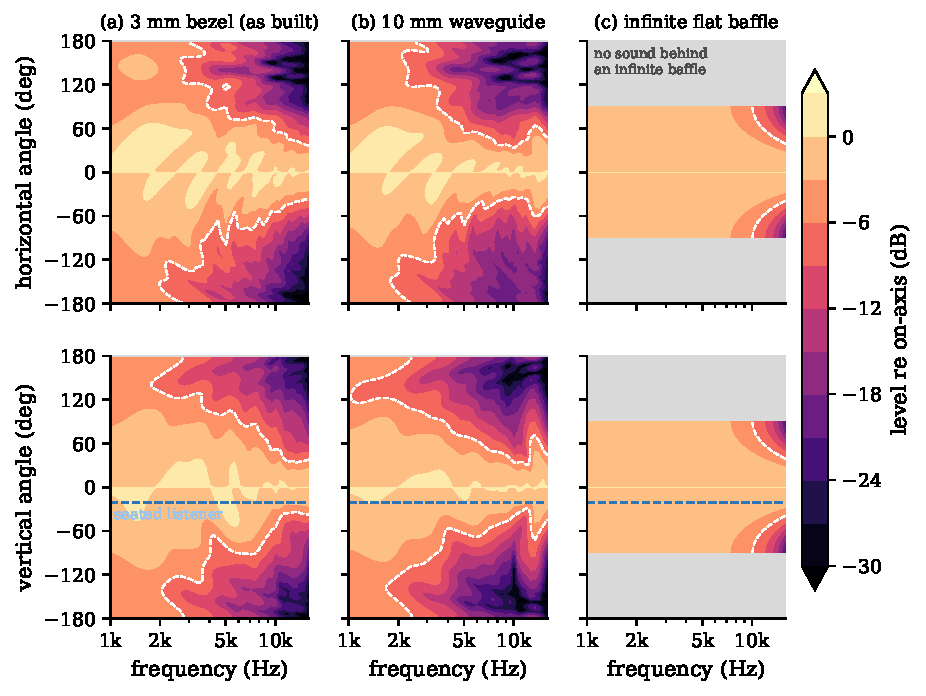
\includegraphics[width=0.8\linewidth]{a2_tweeter_polar_maps_bezel_waveguide_baffle.pdf}
\caption{A2: tweeter polar maps from 1 to \qty{16}{\kilo\hertz}, normalised to on-axis, for the bezel, the waveguide and a flat baffle. The white dashed line is \qty{-6}{\decibel}; the blue dashed line is the seated listener. The waveguide narrows the beam; the bezel behaves like a piston on a curved baffle.}
\label{fig:a2-polar}
\end{figure}

\begin{figure}[htbp]
\centering
\begin{subfigure}[t]{0.9\linewidth}\centering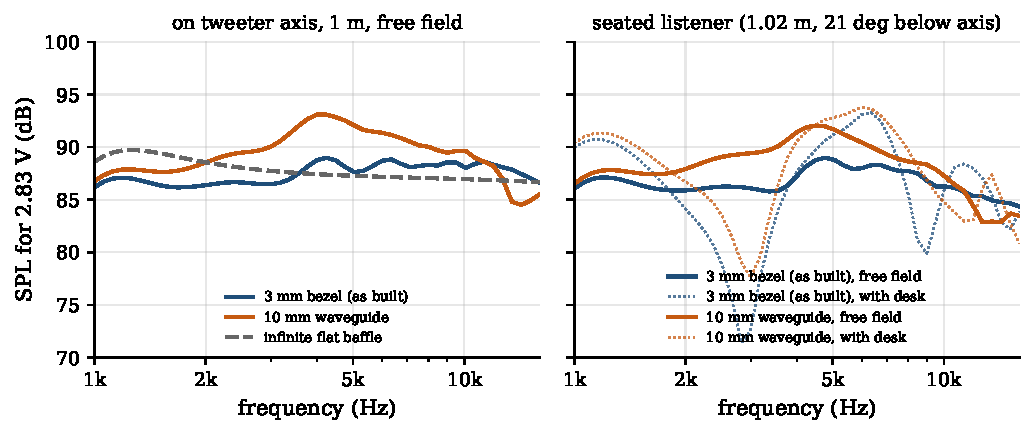
\includegraphics[width=\linewidth]{a2_tweeter_onaxis_and_listening_axis.pdf}\caption{SPL on axis and at the listener, free field and with the desk: the desk notch at \qty{2.8}{\kilo\hertz} dominates.}\end{subfigure}\\[4pt]
\begin{subfigure}[t]{0.9\linewidth}\centering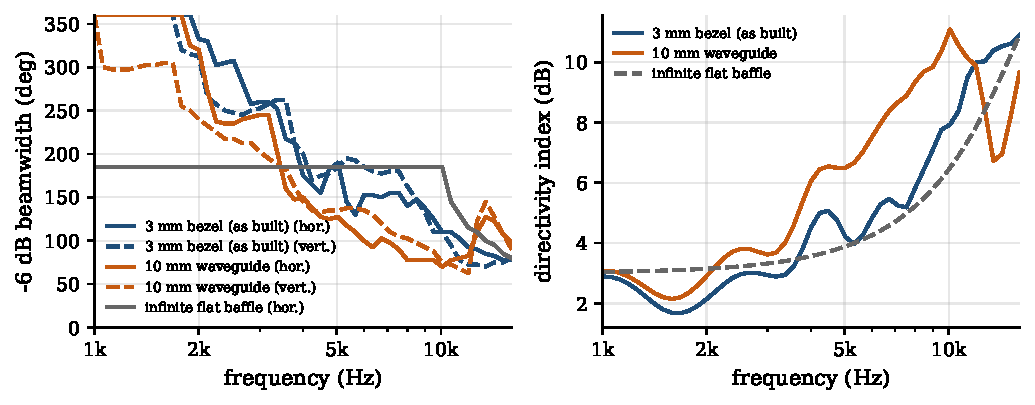
\includegraphics[width=\linewidth]{a2_tweeter_beamwidth_and_DI.pdf}\caption{$-6$~dB beamwidth and directivity index against frequency.}\end{subfigure}
\caption{A2: tweeter response and directivity.}
\label{fig:a2-resp}
\end{figure}

\subsubsection{A3: Woofer baffle step, diffraction and tunnel}\label{sec:a3}

\textbf{Question.} How large are the baffle step and the diffraction ripple on the narrow, round front? And does the \qty{14}{\milli\metre} tunnel through the baffle land matter?

\textbf{Result.}
\begin{itemize}
  \item \textbf{Baffle step.} \qty{-5.6}{\decibel} at low frequency, rising through \qty{-3}{\decibel} at \qty{643}{\hertz}. On the round front it is a smooth shelf, with only \qty{0.36}{\decibel} of ripple from \qty{150}{\hertz} to \qty{2.5}{\kilo\hertz}.
  \item \textbf{The desk gives it back.} The woofers sit \qty{44}{\milli\metre} above the desk, and the reflection adds coherently up to about \qty{2}{\kilo\hertz}. The 15-seat level rises by about \qty{5}{\decibel}, so on a desk no baffle-step boost is needed. That matters because the woofer is the voltage-limited driver. A free-standing preset would need about \qty{+5}{\decibel} below \qty{600}{\hertz}; the microphone auto-EQ can choose between the two presets.
  \item \textbf{The tunnel helps.} It acts as a short, wide horn: \qty{+3.4}{\decibel} in power at \qty{2.5}{\kilo\hertz}, peaking at \qty{+4.7}{\decibel} on axis at \qty{3.8}{\kilo\hertz}. A lumped tube model predicts the same peak height (at \qty{2.7}{\kilo\hertz}). The bump offsets the woofer's voice-coil roll-off, so the tunnel stays as designed.
  \item \textbf{Coverage.} The woofer is still wider than \ang{180} at the \qty{2.5}{\kilo\hertz} crossover.
\end{itemize}

\begin{figure}[htbp]
\centering
\begin{subfigure}[t]{0.49\linewidth}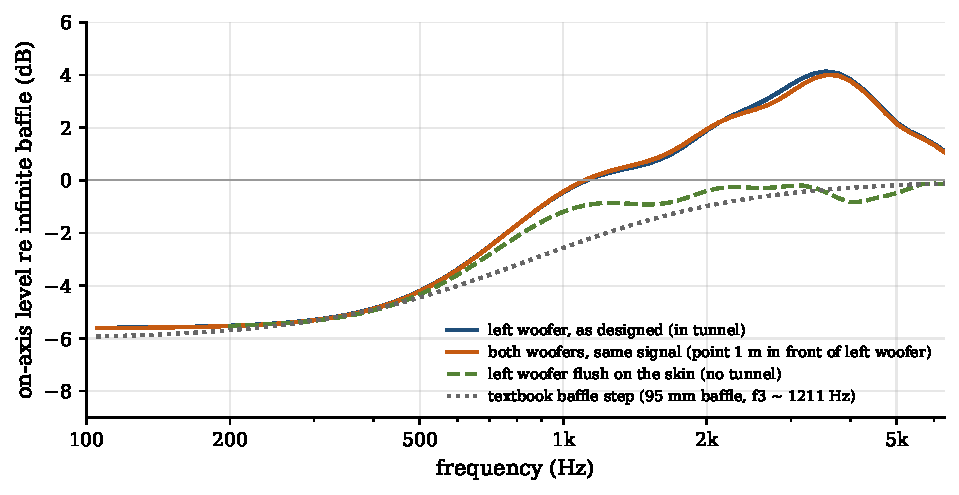
\includegraphics[width=\linewidth]{a3_woofer_baffle_step_and_diffraction.pdf}\caption{On-axis level relative to an infinite baffle: in the tunnel, both woofers, flush, and a textbook step.}\end{subfigure}\hfill
\begin{subfigure}[t]{0.49\linewidth}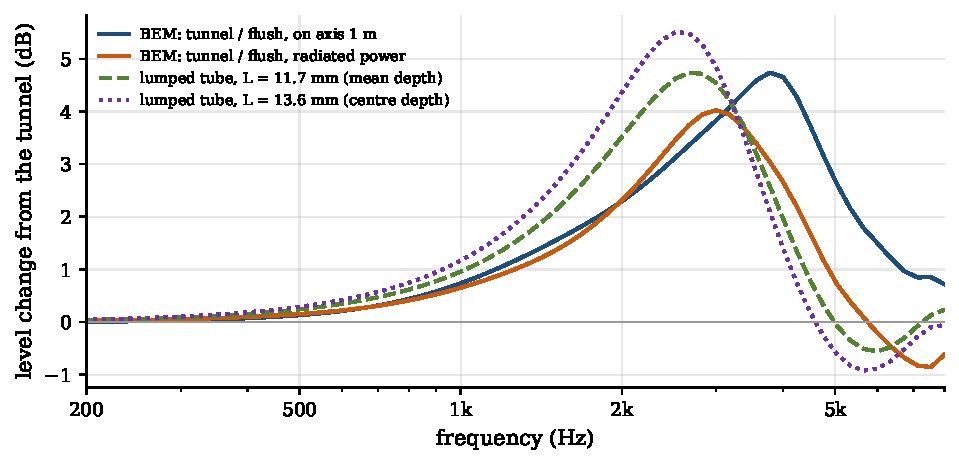
\includegraphics[width=\linewidth]{a3_woofer_tunnel_effect.pdf}\caption{Tunnel effect (BEM on axis and power) against the lumped tube model: a +3--\qty{5}{\decibel} low-Q bump.}\end{subfigure}\\[4pt]
\begin{subfigure}[t]{0.49\linewidth}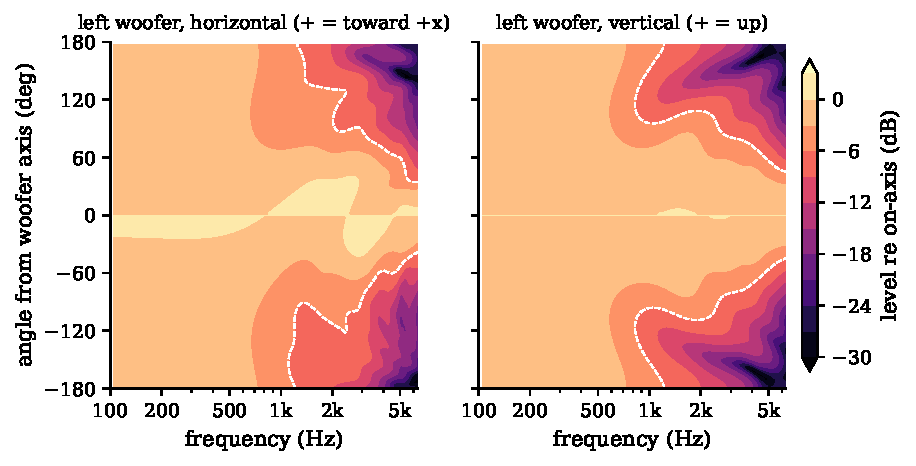
\includegraphics[width=\linewidth]{a3_woofer_polar_maps.pdf}\caption{Woofer polar maps, \qty{100}{\hertz} to \qty{6.3}{\kilo\hertz}.}\end{subfigure}\hfill
\begin{subfigure}[t]{0.49\linewidth}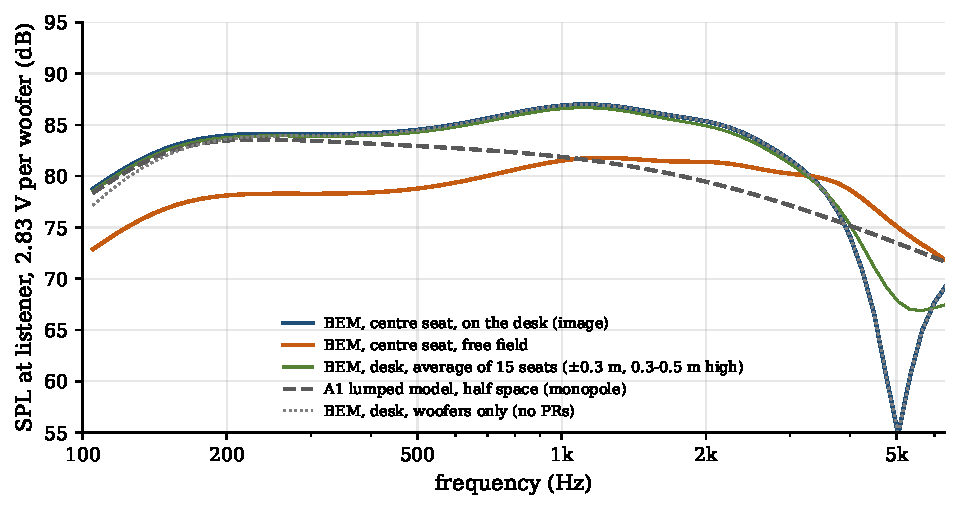
\includegraphics[width=\linewidth]{a3_woofers_and_prs_at_listener.pdf}\caption{Woofers plus PRs at the listener: on the desk, free field, 15-seat average, and A1's model.}\end{subfigure}
\caption{A3: the woofers on the real capsule.}
\label{fig:a3}
\end{figure}

\subsubsection{A4: Panel modes of the printed shell (FEM)}\label{sec:a4}

CalculiX models the five printed parts, tied together, with \qty{40}{\percent} gyroid in the thick features and the drivers and battery as lumped masses: 0.5\,M degrees of freedom, solved in \qty{2}{\minute}.

\textbf{Result.} There are 24 modes below \qty{1}{\kilo\hertz}, starting with ovalling at \qty{269}{\hertz} and a front--back squash at \qty{334}{\hertz}. Their net output stays \textbf{at least \qty{23}{\decibel} below the woofers}, which is under \qty{\pm0.5}{\decibel} of ripple. The heavy woofer frames are what keep the land quiet; without their mass the bare shell has a \qty{529}{\hertz} mode at \qty{-2}{\decibel}. The real risks are local buzz at the top (display, buttons) and a loose battery.

\textbf{Proposed bracing} (not yet in the CAD):
\begin{itemize}
  \item a \qty{1.6}{\milli\metre} centre spine plate in the \qty{2}{\milli\metre} gap between the woofers, which raises the first mode from \qty{269}{\hertz} to \qty{447}{\hertz};
  \item firm battery clamping with tray gussets;
  \item damping pads on the top and bottom flats. Raising the loss factor from 0.03 to 0.1 cuts every resonance by about \qty{10}{\decibel}, more than any rib does.
\end{itemize}

\begin{figure}[htbp]
\centering
\begin{subfigure}[t]{0.49\linewidth}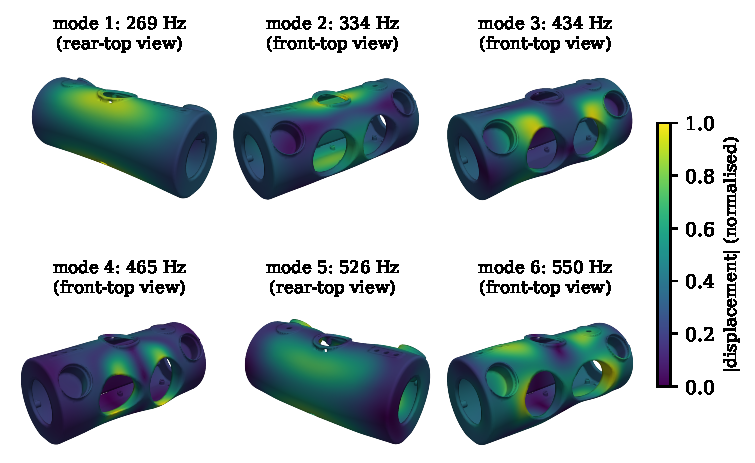
\includegraphics[width=\linewidth]{a4_mode_shapes_main_assembly.pdf}\caption{First six mode shapes: ovalling (\qty{269}{\hertz}), squash (\qty{334}{\hertz}), woofer rocking, rear shell.}\end{subfigure}\hfill
\begin{subfigure}[t]{0.49\linewidth}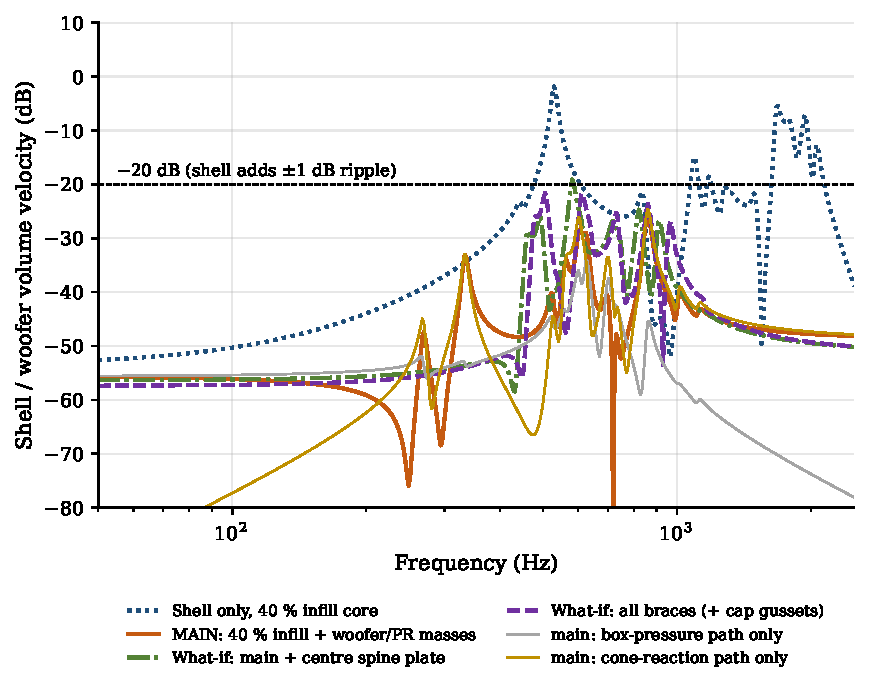
\includegraphics[width=\linewidth]{a4_shell_vs_woofer_output.pdf}\caption{Shell output relative to the woofers: bare shell, as designed, spine plate, all braces.}\end{subfigure}\\[4pt]
\begin{subfigure}[t]{0.49\linewidth}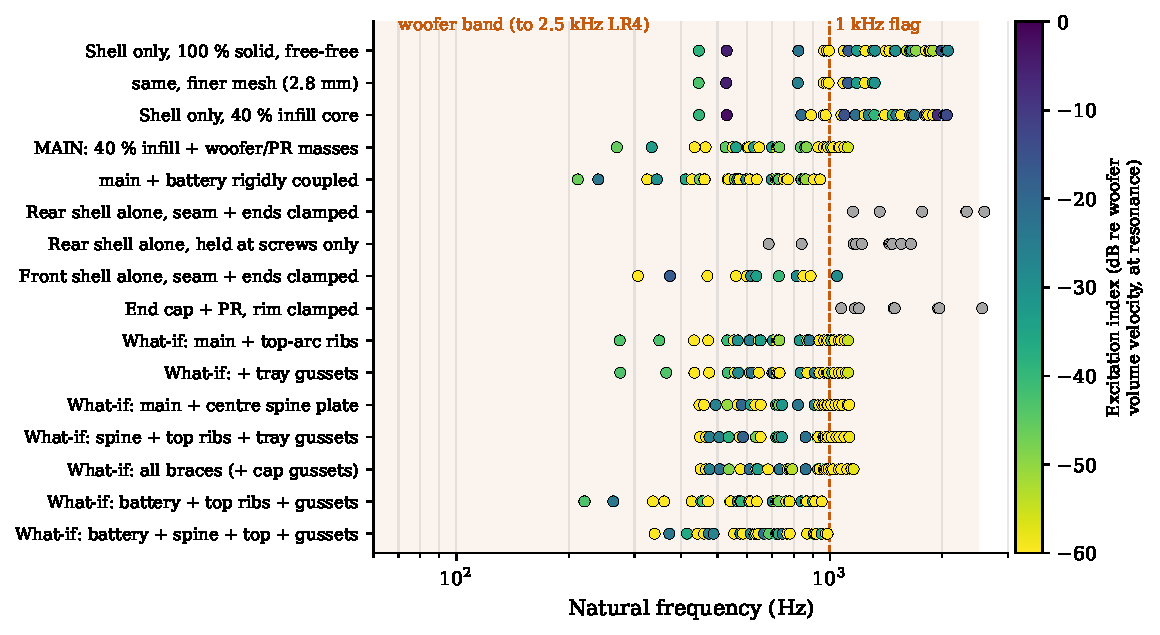
\includegraphics[width=\linewidth]{a4_modal_frequency_map.pdf}\caption{Every mode per case, coloured by how strongly the woofers drive it.}\end{subfigure}\hfill
\begin{subfigure}[t]{0.49\linewidth}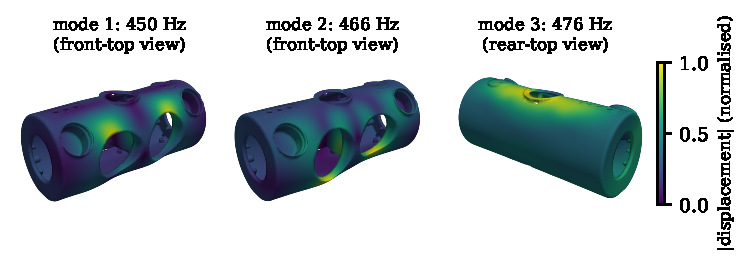
\includegraphics[width=\linewidth]{a4_mode_shapes_all_braces.pdf}\caption{With all braces the lowest mode is about \qty{450}{\hertz}.}\par\medskip
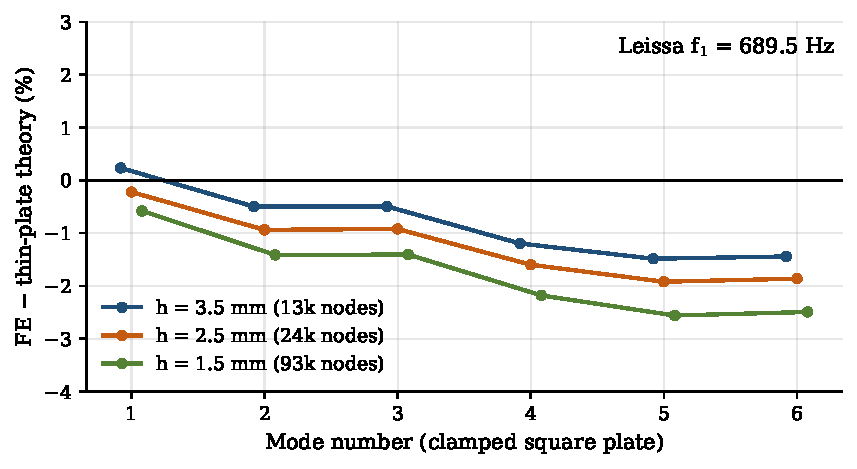
\includegraphics[width=\linewidth]{a4_validation_clamped_plate.pdf}\caption{Validation: clamped plate against Leissa, $\le\qty{1.5}{\percent}$.}\end{subfigure}
\caption{A4: panel modes of the printed enclosure.}
\label{fig:a4}
\end{figure}

\subsubsection{A5: Crossover and system EQ}\label{sec:a5}

A5 combines the A1 velocities, the tweeter model and the BEM transfer functions, with biquads at \qty{96}{\kilo\hertz}, the TAS5805M's DSP rate.

\textbf{Crossover.} LR4 at 2.0, 2.5 and \qty{3.0}{\kilo\hertz} are all well behaved: the drivers are \qty{59}{\milli\metre} apart, less than half a wavelength at \qty{2.5}{\kilo\hertz}, so no deep vertical null forms. Going lower costs tweeter excursion; going higher pushes the woofer into its tunnel bump and voice-coil roll-off. \textbf{The crossover stays at LR4, \qty{2.5}{\kilo\hertz}}, with:
\begin{itemize}
  \item the tweeter trimmed by \qty{-9.7}{\decibel}, normal polarity and delayed by \textbf{\qty{110}{\micro\second}} (11 samples at \qty{96}{\kilo\hertz});
  \item a summed response within \qty{0.05}{\decibel} rms of the ideal in-phase sum.
\end{itemize}

\textbf{System EQ.} Seven biquads were fitted to the 15-seat desk average, with cuts up to \qty{-12}{\decibel} but total boost held to about \qty{+3}{\decibel}, so the desk dip is never filled. The EQ brings the average from \qty{10.8}{\decibel} to \qty{5.0}{\decibel} peak-to-peak; what remains is mostly the desk dip. The two high-frequency filters rest on the rigid-piston model, so they must be confirmed by measurement. All filters (13 biquads on the woofer channel, 9 on the tweeter) are exported in TAS5805M 5.27 format in \repo{sim/acoustics/results/biquads_tas5805m.json}.

\begin{figure}[htbp]
\centering
\begin{subfigure}[t]{0.9\linewidth}\centering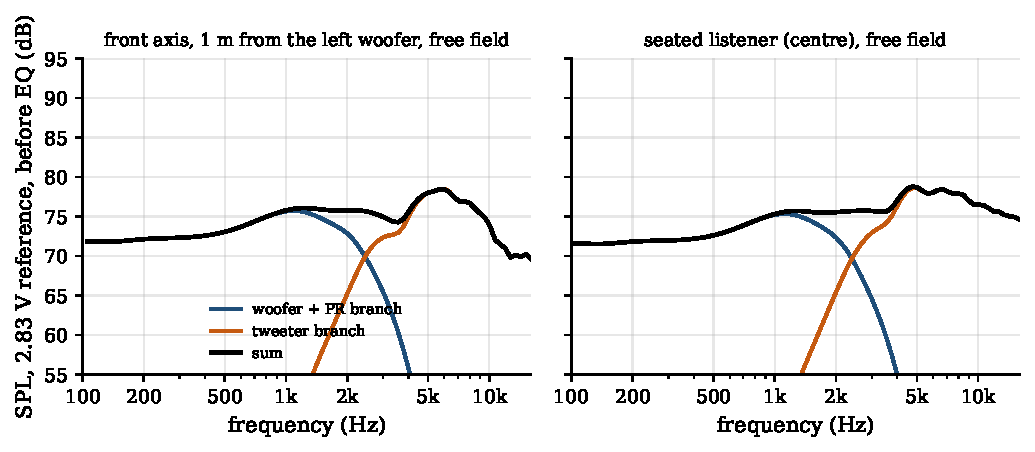
\includegraphics[width=\linewidth]{a5_crossover_branches_lr4_2k5.pdf}\caption{Woofer + PR branch, tweeter branch and sum through LR4 at \qty{2.5}{\kilo\hertz}, before EQ, on the front axis and at the seated listener.}\end{subfigure}\\[4pt]
\begin{subfigure}[t]{0.49\linewidth}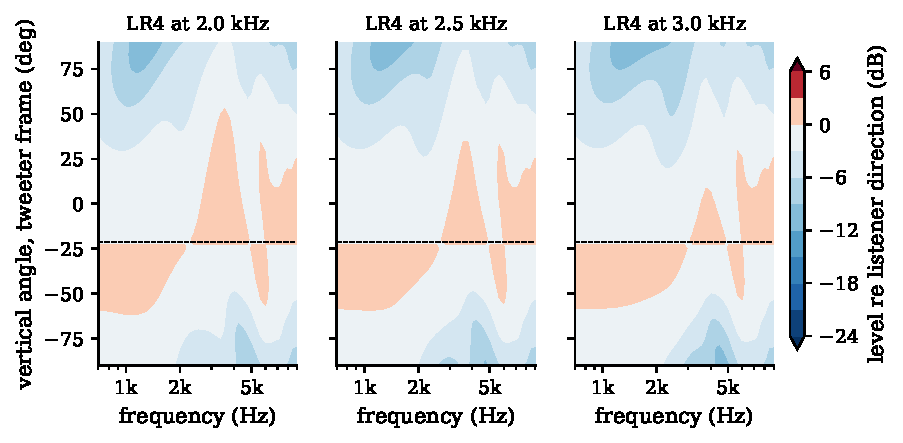
\includegraphics[width=\linewidth]{a5_vertical_lobing_vs_crossover_frequency.pdf}\caption{Vertical lobing for LR4 at 2.0, 2.5 and \qty{3.0}{\kilo\hertz}: no deep null within \ang{-50}\ldots\ang{+10} of the listener.}\end{subfigure}\hfill
\begin{subfigure}[t]{0.49\linewidth}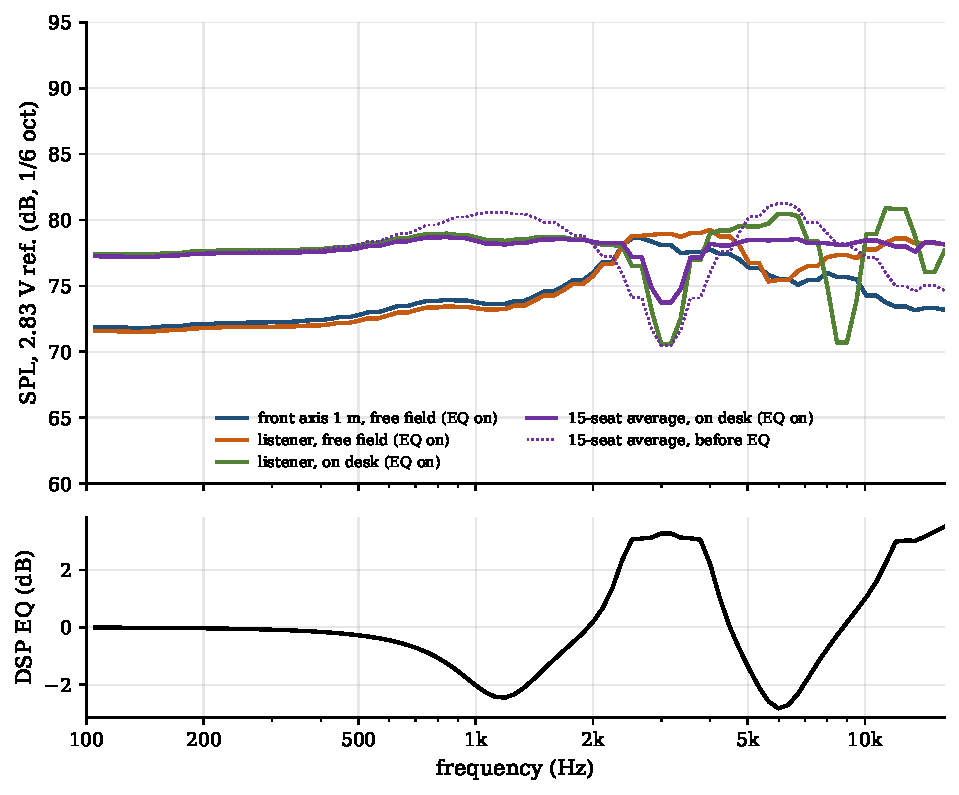
\includegraphics[width=\linewidth]{a5_system_response_per_side_with_eq.pdf}\caption{Per-side response with EQ at four positions, and the EQ curve.}\end{subfigure}\\[4pt]
\begin{subfigure}[t]{0.6\linewidth}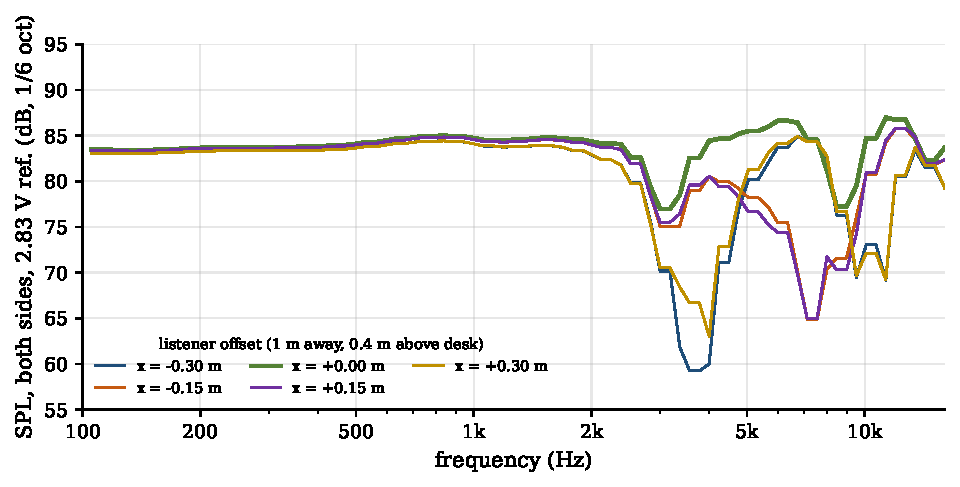
\includegraphics[width=\linewidth]{a5_stereo_pair_mono_at_seats.pdf}\caption{Both sides with a mono signal at five seats: comb filtering above \qty{3}{\kilo\hertz} off-centre, normal for any stereo pair.}\end{subfigure}
\caption{A5: crossover and system response.}
\label{fig:a5}
\end{figure}

\begin{checked}
\begin{itemize}[leftmargin=1.2em,itemsep=1pt]
  \item \textbf{A1:} the sealed-box resonance matches the closed form (\qty{140.03}{\hertz} against \qty{140.04}{\hertz}), and the model matches electroacPy within \qty{0.013}{\decibel} SPL, \qty{0.22}{\percent} impedance and \qty{0.025}{\decibel} excursion.
  \item \textbf{BEM:}
  \begin{itemize}[leftmargin=1.2em,itemsep=0pt]
    \item piston on a sphere against the exact series: \qty{0.010}{\decibel} at \qty{1}{\kilo\hertz}, \qty{0.34}{\decibel} at \qty{8}{\kilo\hertz};
    \item CHIEF against Burton--Miller on the real capsule: within \qty{0.15}{\decibel} (tweeter);
    \item \textbf{mesh convergence at \qty{5}{\kilo\hertz}:} the first, uniform mesh was off by up to \qty{1.3}{\decibel} at the tweeter. Doubling the CHIEF points did not help, which showed the error came from the mesh, so the tweeter zone was refined to \qty{2.8}{\milli\metre} and everything re-run. Production meshes are within \qty{0.3}{\decibel} of a finer reference;
    \item the BEM bass level at the listener matches A1 within \qty{0.43}{\decibel}, and left and right tweeters mirror within a median \qty{0.26}{\decibel}.
  \end{itemize}
  \item \textbf{A4:} clamped plate against Leissa within \qty{1.5}{\percent}; mesh refinement moves the first eight modes by $\le\qty{0.4}{\percent}$.
  \item \textbf{A5:} the LR4 sum is within \qty{0.05}{\decibel} of ideal; every encoded TAS5805M word decodes back within $2^{-26}$.
\end{itemize}
\end{checked}

% =====================================================================
\FloatBarrier
\subsection{Circuits and power distribution (SPICE, PDN)}\label{sec:spice}

All circuit simulations ran in ngspice and Python \src{sim/spice/README.md}. TI publishes an unencrypted transient model of the TPS61178, and it runs unmodified in ngspice.

\subsubsection{S1 and S7: the boost loop and the amplifier rail}\label{sec:s1}\label{sec:s7}

\textbf{Finding 1: stable, but soft.} The loop has at least \ang{64.8} of phase margin everywhere. With \qty{1.5}{\milli\farad} on the rail, though, it crosses over at only about \qty{250}{\hertz}. The rail impedance therefore peaks at \qtyrange{0.46}{0.57}{\ohm} near \qty{150}{\hertz}, 3.4--$4.2\times$ the \qty{0.137}{\ohm} target, exactly where bass draws current. A \qty{5}{\ampere} bass transient would sag PVDD by more than \qty{2}{\volt}. Raising $R_c$ to \qty{100}{\kilo\ohm} (ECO-001 \#1) brings the peak to \qty{0.16}{\ohm} and cuts a load-step dip from \qty{0.97}{\volt} to \qty{0.34}{\volt}, at no cost. The worst impedance on the board sits at \qty{150}{\hertz}, not at gigahertz. The +3V3 rail meets its \qty{0.30}{\ohm} target with margin.

\textbf{Finding 2: start-up windup.} The internal soft start finishes in \qty{3.2}{\milli\second}, but charging the bank takes \qty{11}{\milli\second} at the current limit. The error amplifier winds up, and PVDD overshoots to \qty{19.4}{\volt} (typical) or to the \qty{21}{\volt} OVP. A faster loop does not help. The fix is a firmware soft start through the trim network (ECO-001 \#2).

\begin{figure}[htbp]
\centering
\begin{subfigure}[t]{0.49\linewidth}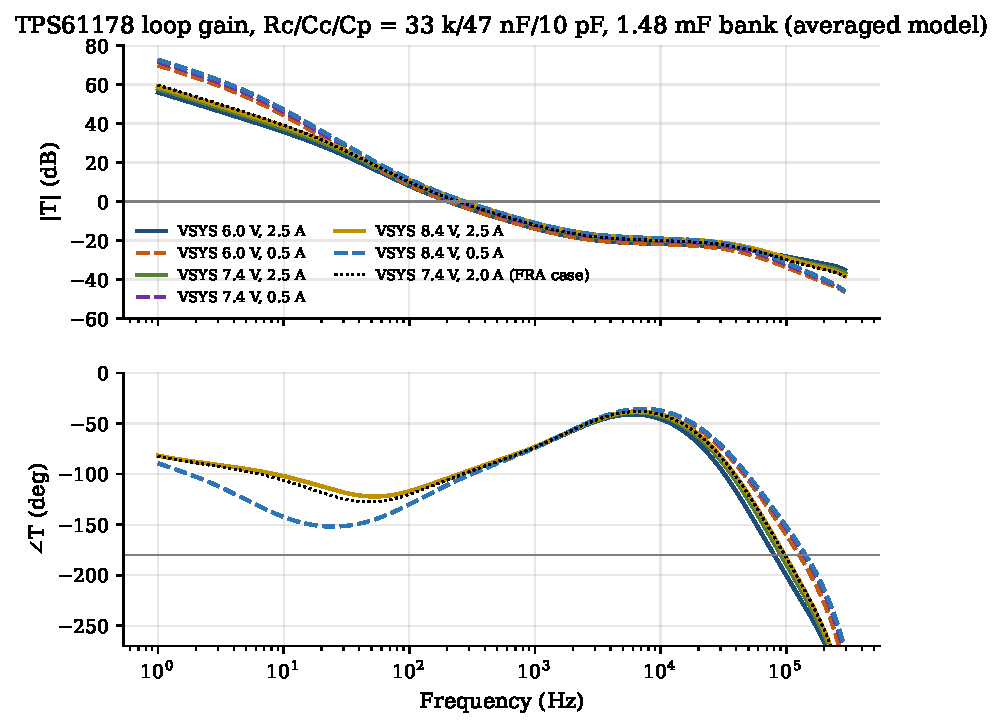
\includegraphics[width=\linewidth]{s1_loop_bode.pdf}\caption{Loop gain across input voltage and load.}\end{subfigure}\hfill
\begin{subfigure}[t]{0.49\linewidth}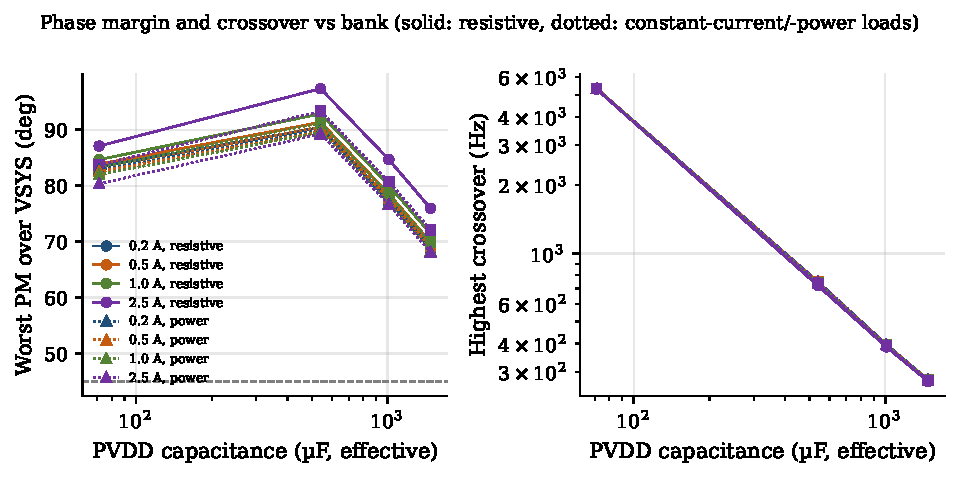
\includegraphics[width=\linewidth]{s1_loop_margins.pdf}\caption{Worst phase margin and crossover against PVDD capacitance.}\end{subfigure}\\[4pt]
\begin{subfigure}[t]{0.49\linewidth}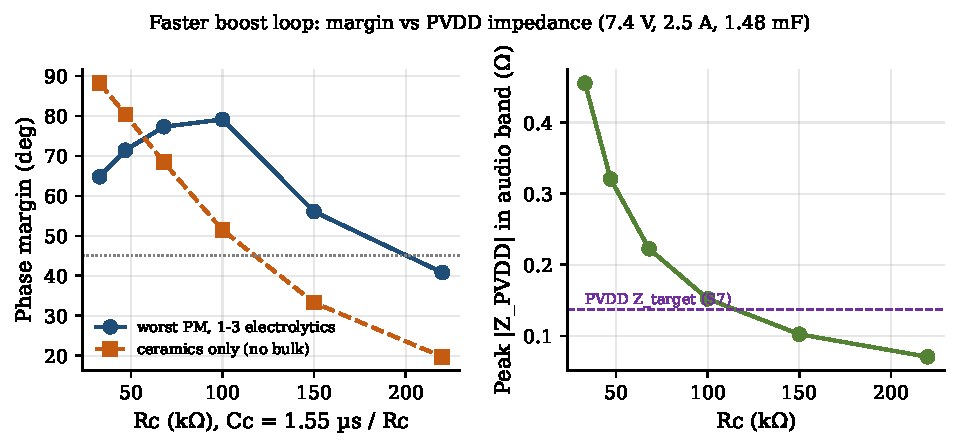
\includegraphics[width=\linewidth]{s1_compensation_options.pdf}\caption{$R_c$ sweep: \qty{100}{\kilo\ohm} reaches the impedance target with PM $\ge\ang{79}$.}\end{subfigure}\hfill
\begin{subfigure}[t]{0.49\linewidth}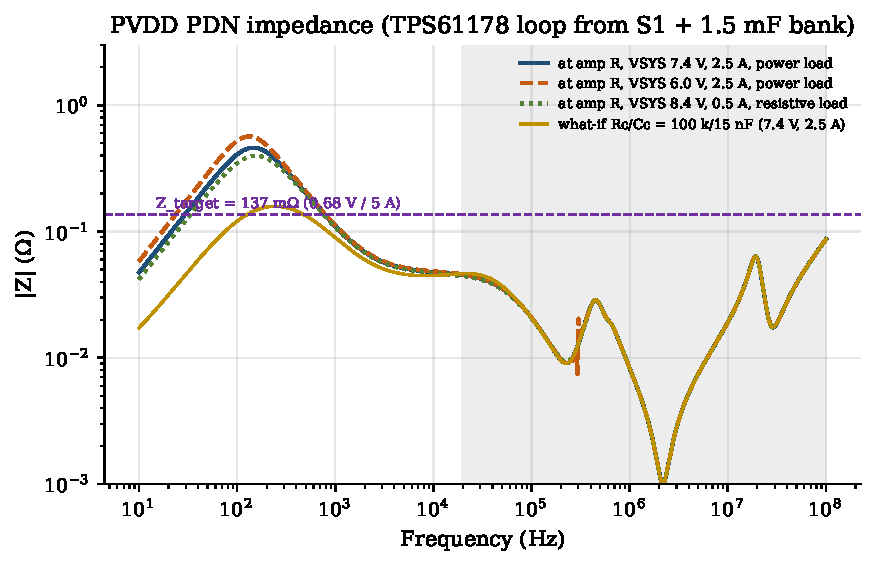
\includegraphics[width=\linewidth]{s7_pdn_pvdd.pdf}\caption{PVDD impedance at the amplifier: the \qty{150}{\hertz} peak and the ECO fix against the target.}\end{subfigure}\\[4pt]
\begin{subfigure}[t]{0.49\linewidth}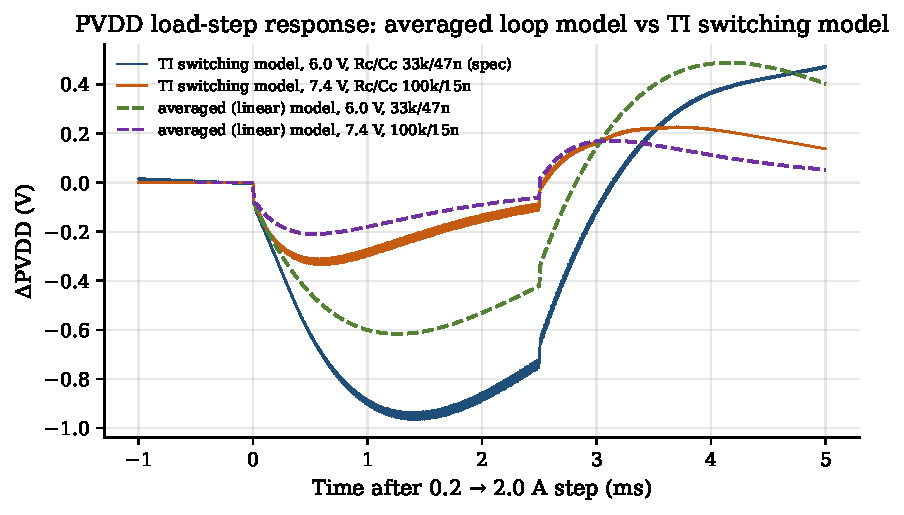
\includegraphics[width=\linewidth]{s1_loadstep.pdf}\caption{\qtyrange{0.2}{2}{\ampere} step: averaged model against TI's switching model.}\end{subfigure}\hfill
\begin{subfigure}[t]{0.49\linewidth}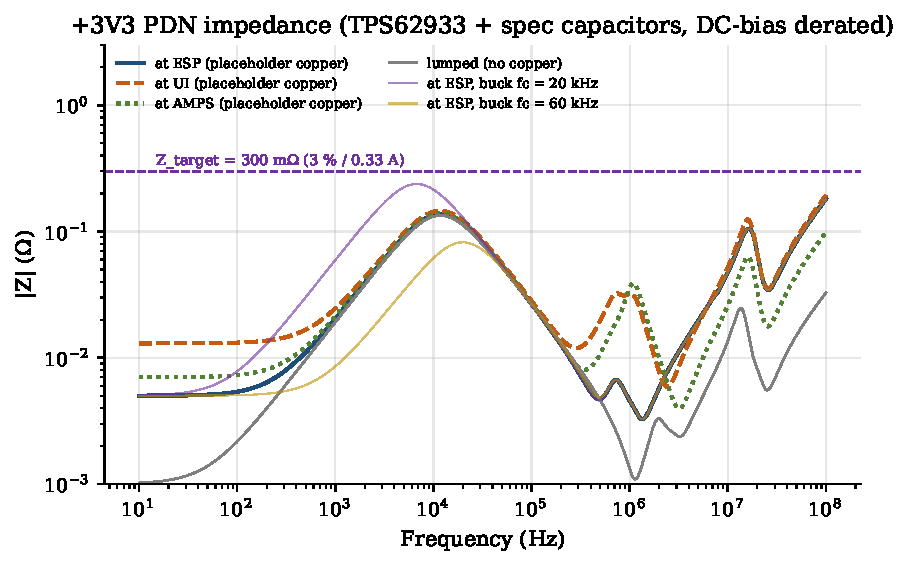
\includegraphics[width=\linewidth]{s7_pdn_3v3.pdf}\caption{+3V3 impedance: within its \qty{0.30}{\ohm} target.}\end{subfigure}
\caption{S1/S7: the boost loop and the rails. Small-signal stability is fine; the problem is impedance in the bass band.}
\label{fig:s1}
\end{figure}

\begin{figure}[htbp]
\centering
\begin{subfigure}[t]{0.49\linewidth}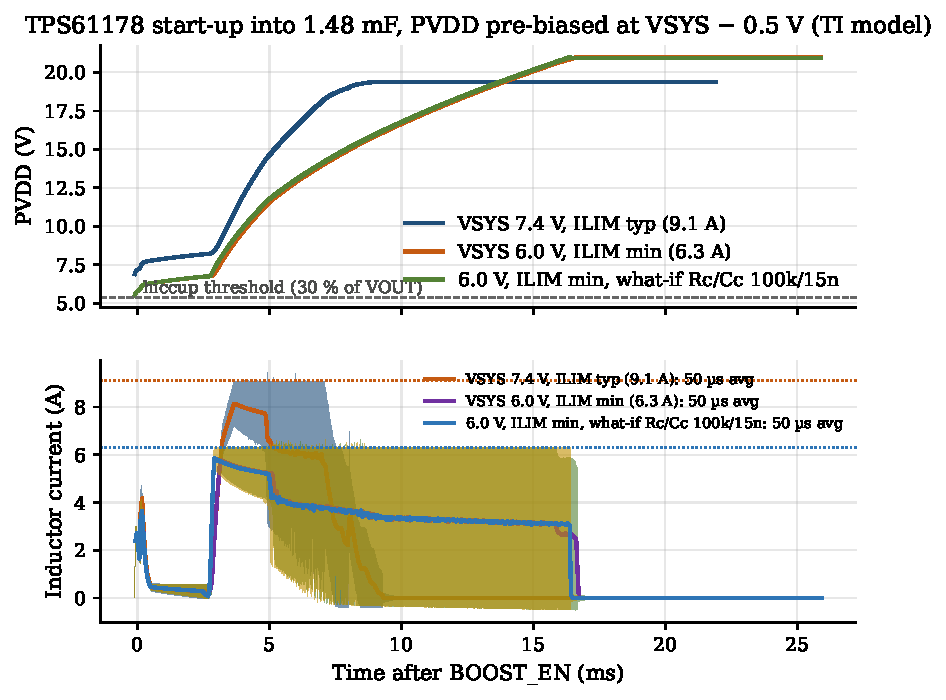
\includegraphics[width=\linewidth]{s1_startup.pdf}\caption{Start-up into \qty{1.5}{\milli\farad}: \qty{11}{\milli\second} in current limit, then overshoot from windup.}\end{subfigure}\hfill
\begin{subfigure}[t]{0.49\linewidth}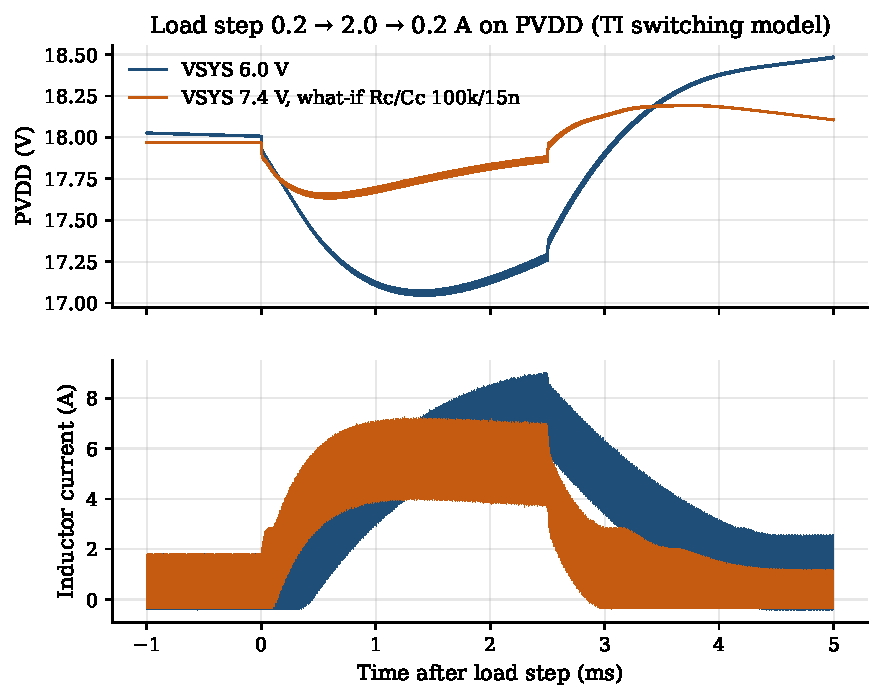
\includegraphics[width=\linewidth]{s1_loadstep_switching.pdf}\caption{Load step and release in the TI model; PFM cannot sink current, so the release overshoots.}\end{subfigure}
\caption{S1: large-signal behaviour that the datasheet equations hide.}
\label{fig:s1-large}
\end{figure}

\subsubsection{S2: Class-D output filter into the real drivers}\label{sec:s2}

Into the real tweeter impedance, the \qty{10}{\micro\henry}/\qty{1}{\micro\farad} filter droops \qty{2.2}{\decibel} by \qty{20}{\kilo\hertz}. The spec had estimated \qty{0.44}{\decibel} with a resistor load, and the fix is a \qty{+2}{\decibel} shelf (ECO-001 \#5). Into the woofer's \qty{0.61}{\milli\henry}, the filter is almost unloaded and peaks at \qty{59}{\kilo\hertz} ($Q\approx14$), which is harmless after the crossover. With the limiters, inductor current stays at or below \qty{2.7}{\ampere}. A hard-clipped tweeter reaches \qty{5.41}{\ampere}, past the \qty{5}{\ampere} trip, so the tweeter limiter is mandatory.

\begin{figure}[htbp]
\centering
\begin{subfigure}[t]{0.49\linewidth}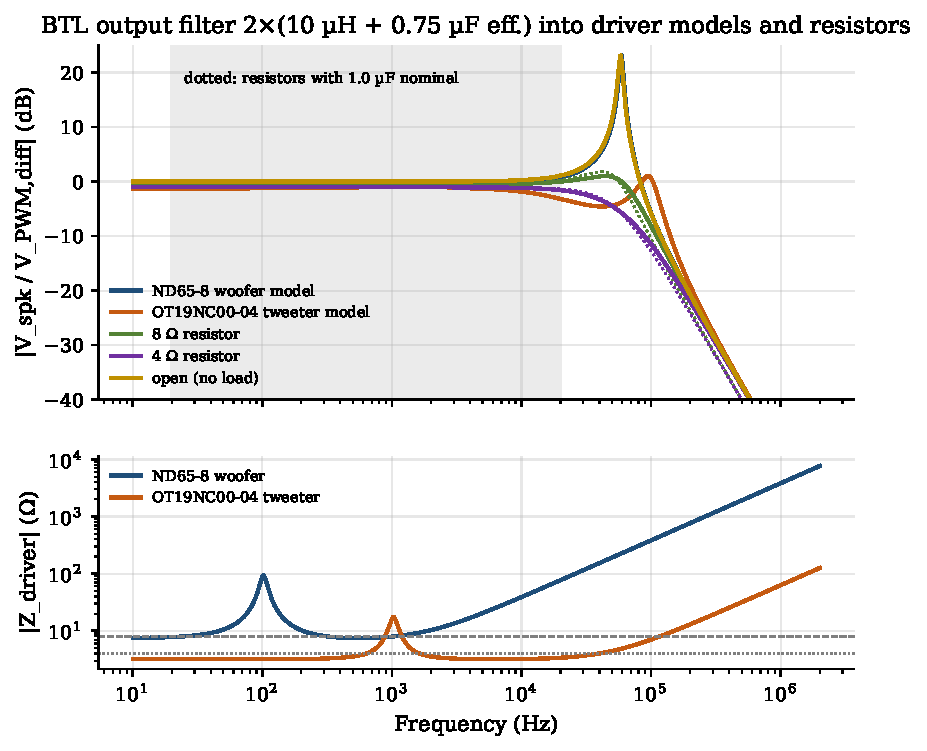
\includegraphics[width=\linewidth]{s2_filter_response.pdf}\caption{Filter into the driver models and into resistors.}\end{subfigure}\hfill
\begin{subfigure}[t]{0.49\linewidth}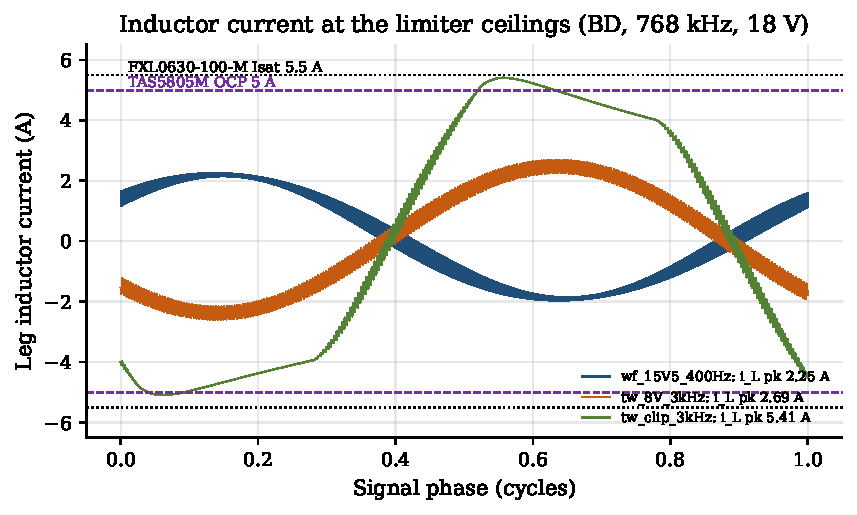
\includegraphics[width=\linewidth]{s2_inductor_peaks.pdf}\caption{Peak inductor current at the limiter ceilings and with a clipped tweeter.}\par\medskip
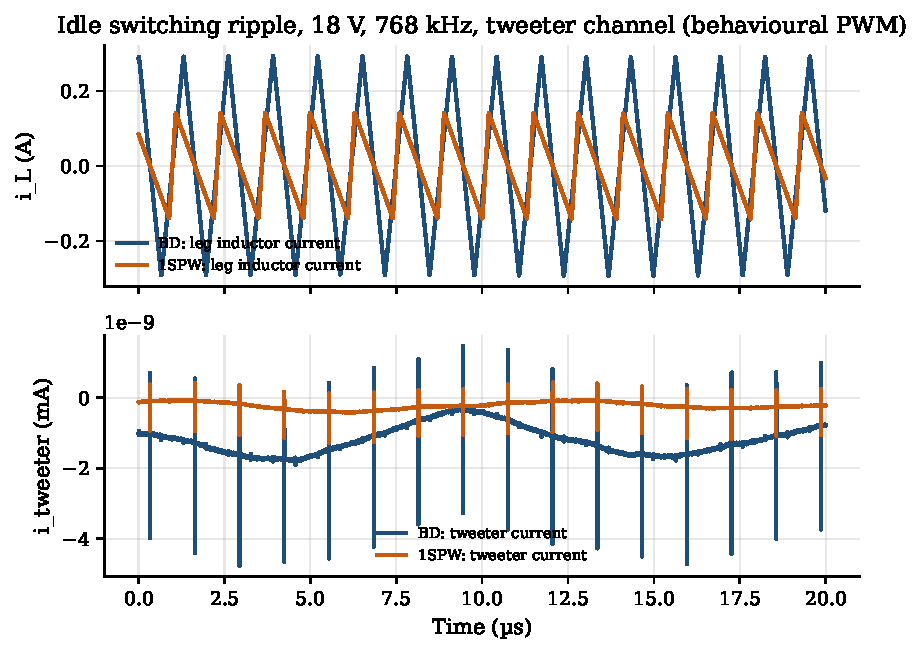
\includegraphics[width=\linewidth]{s2_idle_ripple.pdf}\caption{Idle ripple circulates in the filter capacitors, not the drivers.}\end{subfigure}
\caption{S2: a loudspeaker is not a resistor.}
\label{fig:s2}
\end{figure}

\subsubsection{S3--S5: NTC window, PVDD trim, ESP32 reset}\label{sec:s3}\label{sec:s4}\label{sec:s5}

\begin{itemize}
  \item \textbf{S3, NTC.} The charge window is \qtyrange{2.0}{60.8}{\degreeCelsius}, and an open NTC fails safe. With the charger's defaults it would keep charging from 45 to \qty{61}{\degreeCelsius}, so firmware stops it at \qty{45}{\degreeCelsius} (ECO-001 \#6).
  \item \textbf{S4, trim.} PVDD trims from \qty{18.0}{\volt} down to \qty{12.2}{\volt}. The curve sits \qty{0.3}{\volt} below the hand table, because the diode drops \qty{0.35}{\volt} at microamps, not \qty{0.45}{\volt}. It settles in \qtyrange{70}{110}{\milli\second}, and PWM ripple at the feedback node is below \qty{0.5}{\micro\volt}.
  \item \textbf{S5, reset.} With \qty{1}{\micro\farad}, esptool's auto-reset fails if the host leaves more than about \qty{2.5}{\milli\second} between its DTR and RTS requests. \qty{2.2}{\micro\farad} doubles the tolerance to \qty{5}{\milli\second} and also stops EN rising before the rail is valid (ECO-001 \#4). All strap levels read correctly.
\end{itemize}

\begin{figure}[htbp]
\centering
\begin{subfigure}[t]{0.49\linewidth}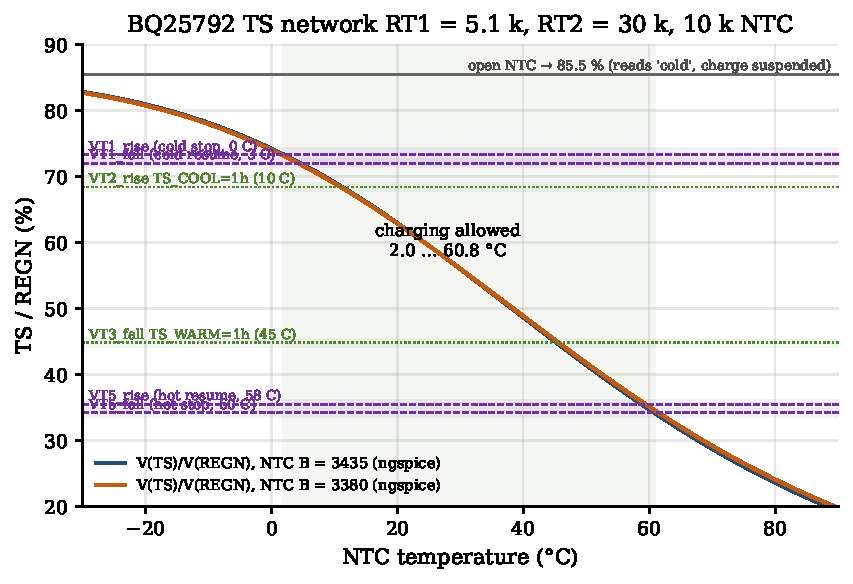
\includegraphics[width=\linewidth]{s3_ntc_window.pdf}\caption{S3: TS/REGN against temperature with the charger's thresholds.}\end{subfigure}\hfill
\begin{subfigure}[t]{0.49\linewidth}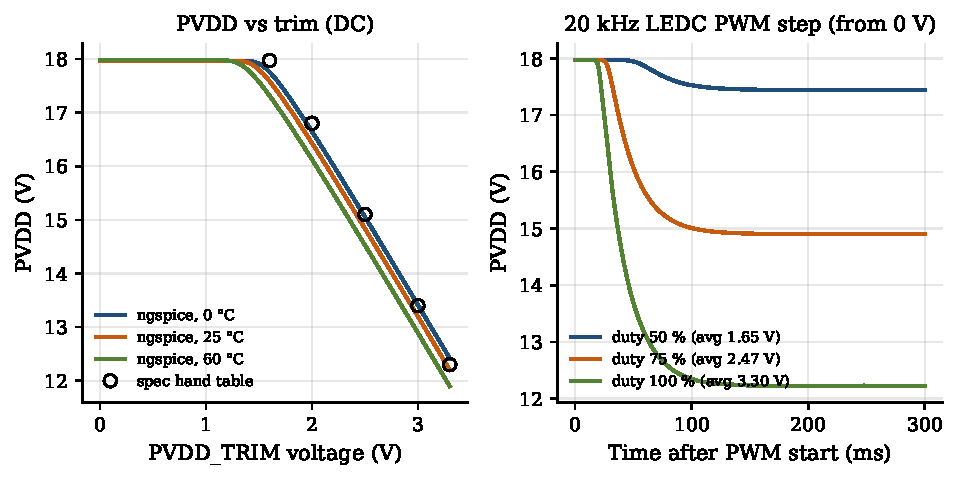
\includegraphics[width=\linewidth]{s4_pvdd_trim.pdf}\caption{S4: PVDD against trim voltage, and PWM transients.}\end{subfigure}\\[4pt]
\begin{subfigure}[t]{0.49\linewidth}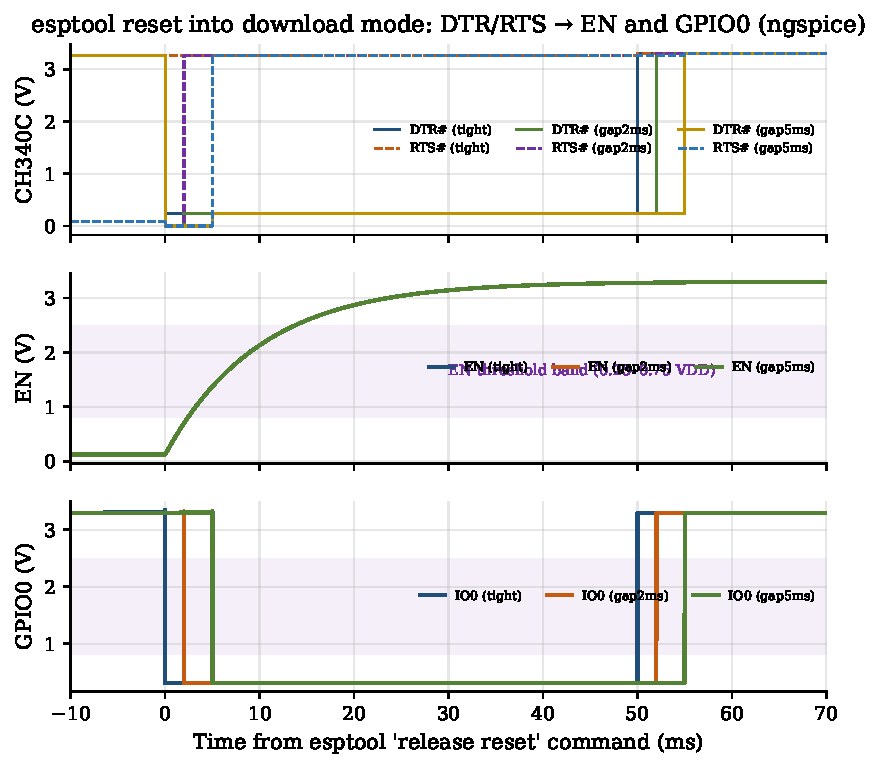
\includegraphics[width=\linewidth]{s5_autoreset.pdf}\caption{S5: auto-reset for the tight sequence and \qtylist{2;5}{\milli\second} gaps.}\end{subfigure}\hfill
\begin{subfigure}[t]{0.49\linewidth}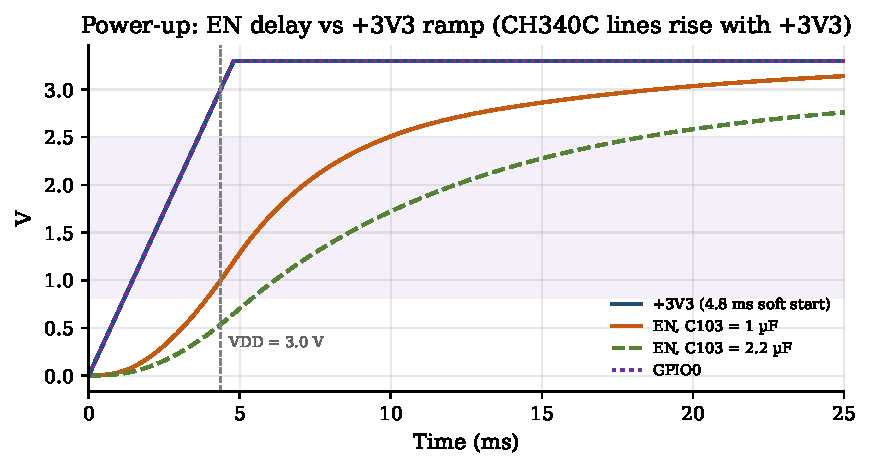
\includegraphics[width=\linewidth]{s5_powerup.pdf}\caption{S5: power-up with \qty{1}{\micro\farad} against \qty{2.2}{\micro\farad}.}\end{subfigure}
\caption{S3--S5: small circuits with real consequences.}
\label{fig:s3s5}
\end{figure}

\subsubsection{S6: Signal integrity on the UI flat cable}\label{sec:s6}

A 2-D field solver gives the 20-way FFC with ground on both sides of the clock as a $\approx\qty{107}{\ohm}$ line, twice what the ``\qty{33}{\ohm} for \qty{50}{\ohm}'' rule of thumb assumes. With \qty{33}{\ohm} source resistors, SCLK at \qty{40}{\mega\hertz} overshoots by \qtyrange{0.7}{1.1}{\volt}, enough to conduct the receiver's ESD diodes. With \qty{68}{\ohm} the overshoot is \qty{0.2}{\volt} at worst, and the clock can safely reach \qty{53}{\mega\hertz} (ECO-001 \#3). Crosstalk stays below the input-low threshold. The simulation used a \qty{200}{\milli\metre} cable; the build uses \qty{100}{\milli\metre}, so the results are conservative.

\begin{figure}[htbp]
\centering
\begin{subfigure}[t]{0.49\linewidth}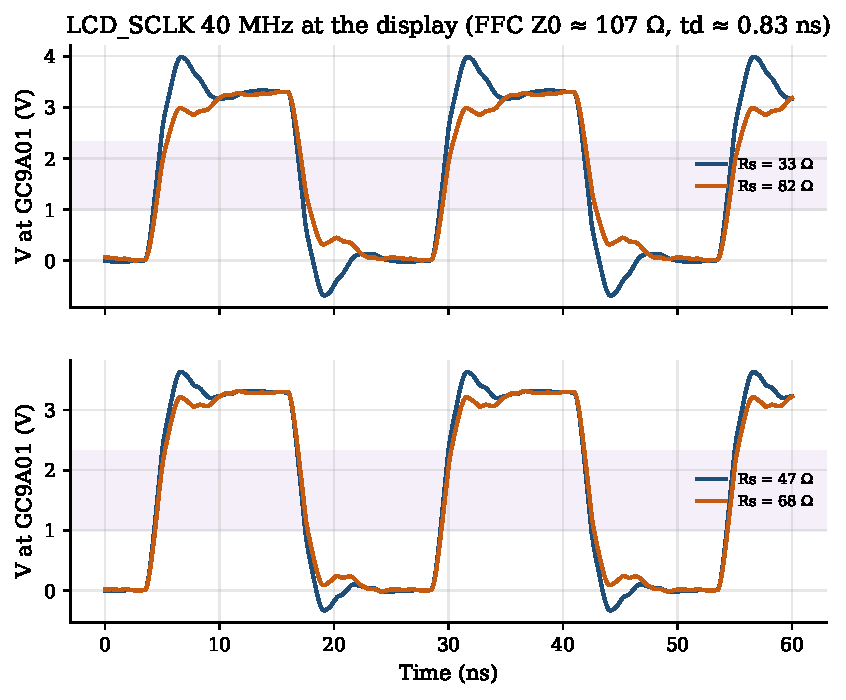
\includegraphics[width=\linewidth]{s6_sclk_40MHz.pdf}\caption{SCLK at the display for 33--\qty{82}{\ohm}.}\end{subfigure}\hfill
\begin{subfigure}[t]{0.49\linewidth}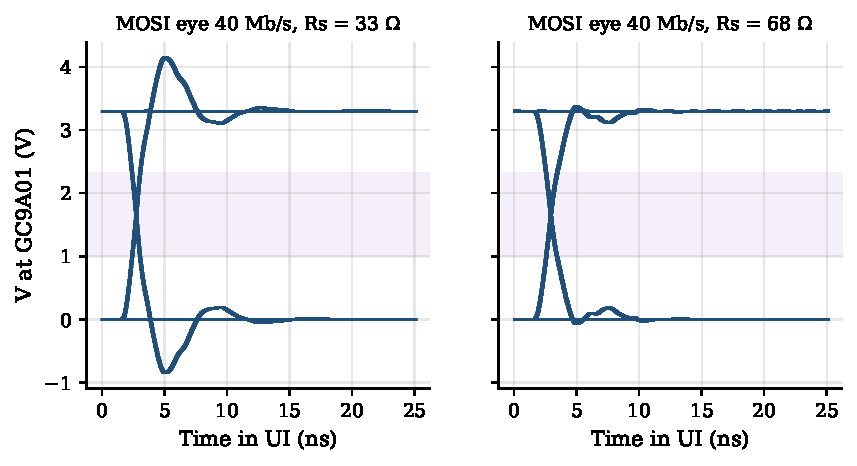
\includegraphics[width=\linewidth]{s6_mosi_eye.pdf}\caption{MOSI eye at \qty{40}{\mega\bit\per\second}, \qty{33}{\ohm} against \qty{68}{\ohm}.}\end{subfigure}\\[4pt]
\begin{subfigure}[t]{0.49\linewidth}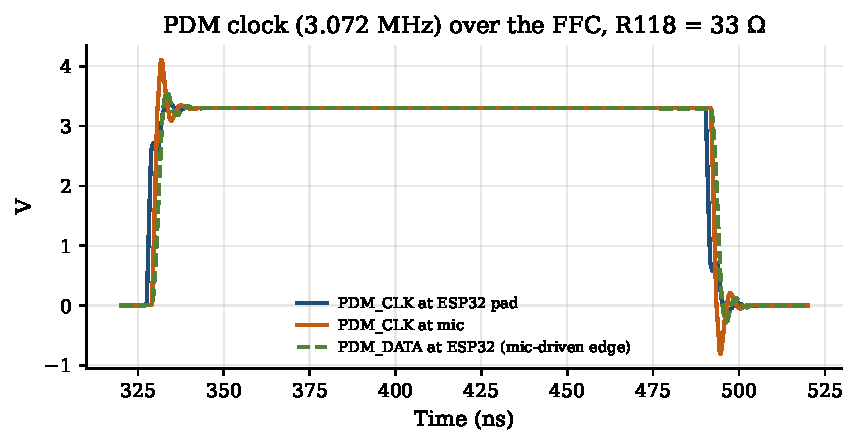
\includegraphics[width=\linewidth]{s6_pdm.pdf}\caption{PDM clock and the returning data edge.}\end{subfigure}\hfill
\begin{subfigure}[t]{0.49\linewidth}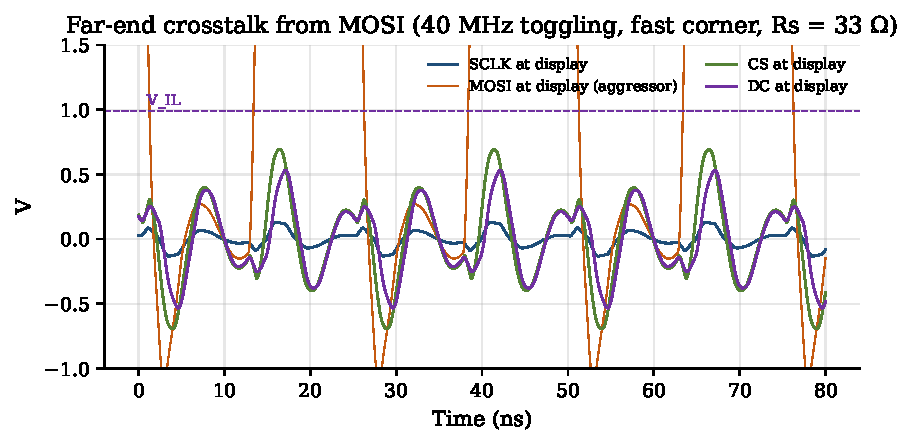
\includegraphics[width=\linewidth]{s6_crosstalk.pdf}\caption{Far-end crosstalk with MOSI toggling.}\end{subfigure}
\caption{S6: a ribbon cable is a transmission line.}
\label{fig:s6}
\end{figure}

\begin{checked}
\begin{itemize}[leftmargin=1.2em,itemsep=1pt]
  \item \textbf{S1:} hand crossover \qty{228}{\hertz} against \qty{247}{\hertz} modelled; hand impedance peak \qty{0.44}{\ohm} against \qty{0.46}{\ohm}. The averaged and switching models agree in shape; the switching model dips $1.6\times$ deeper because the error amplifier is slew-limited.
  \item \textbf{S2:} filter corner (\qty{50.3}{\kilo\hertz}) and idle ripple (\qty{0.585}{\ampere} against \qty{0.586}{\ampere}) match hand calculation.
  \item \textbf{S3:} TI's reference network is reproduced within 0.5 percentage points of REGN.
  \item \textbf{S6:} the field solver matches conformal mapping within \qty{0.1}{\percent}.
  \item \textbf{S7:} the PVDD peak matches the hand value.
  \item \textbf{Not done:} the injection loop-gain measurement and one load-step corner stalled in ngspice and were dropped. Both moved to the bench list.
\end{itemize}
\end{checked}
\FloatBarrier

\section{Firmware requirements derived from analysis}\label{sec:firmware-req}

Several hardware decisions only work if the firmware does its part. The removal of the boost disconnect FET, for example, relies on the charger's over-current trip, and that trip is a register setting. The SPICE runs, the release reviews and the ECOs together produced the contract in \cref{tab:firmware-req}. Items 1--7 protect hardware and must exist before the first battery power-up with amplifiers. The spec's firmware notes are the authoritative list \src{docs/spec_power.md} §7 \src{docs/spec_signal.md}.

{\small
\setlength{\tabcolsep}{4pt}
\begin{longtable}{@{}r >{\raggedright\arraybackslash}p{0.43\linewidth} >{\raggedright\arraybackslash}p{0.33\linewidth} >{\raggedright\arraybackslash}p{0.13\linewidth}@{}}
\caption{Firmware requirements, grouped by subsystem. ``Origin'' names the analysis that produced each one.}\label{tab:firmware-req}\\
\toprule
\# & Requirement & Why & Origin \\
\midrule
\endfirsthead
\toprule \# & Requirement & Why & Origin \\ \midrule
\endhead
\bottomrule
\endfoot
\multicolumn{4}{@{}l}{\textbf{Charger (BQ25792, 0x6B): first thing at every boot}} \\
1 & Write SFET\_PRESENT = 1, EN\_BATOC = 1, WATCHDOG = 0 (or re-arm all three and ICHG on every WD\_FLAG). Read back; on failure keep BOOST\_EN low and report a fault & The \qty{9.3}{\ampere} battery over-current trip is the only fast PVDD short protection (no disconnect FET). A watchdog expiry or REG\_RST clears EN\_BATOC & Review S1; ECO-002 \#7 \\
2 & Write ICHG at boot: $\le\qty{2.5}{\ampere}$ for the \qty{5}{\ampere\hour} pack, $\le\qty{1.75}{\ampere}$ for the \qty{3.5}{\ampere\hour} fallback & POR/watchdog default is \qty{2}{\ampere}, 0.57C on the fallback pack & Review S3 \\
3 & JEITA: stop charging above \qty{45}{\degreeCelsius} & Hardware window runs to \qty{60.8}{\degreeCelsius}; POR keeps charging from 45 to \qty{61}{\degreeCelsius} & S3; ECO-001 \#6 \\
4 & AUTO\_INDET\_EN = 0; IINDPM = CH224Q reg 0x50 $\times$ \qty{50}{\milli\ampere}, capped at \qty{3}{\ampere}; $\le$\qtyrange{0.5}{1.5}{\ampere} without PD & D+/D$-$ are not connected; blank firmware draws up to \qty{2.9}{\ampere} from any \qty{5}{\volt} port & spec\_power §2.3; review L1 \\
5 & Read TS in battery-only mode and stop playback above the pack limit & No hardware discharge over-temperature cut-off & Review S6 \\
6 & Never request \qty{28}{\volt} EPR from the CH224Q & Isolator gate would see \qty{14}{\volt} ($>\pm\qty{12}{\volt}$); BQ VBUS max \qty{24}{\volt} & spec\_power §1.3 \\
\addlinespace
7 & If C720/C721 are ever fitted: C721 $\ge10\times$ C720, never fit R710, and wait until VSYS $\approx$ VBAT ($\Delta V<\qty{50}{\milli\volt}$ on the charger ADC) before BOOST\_EN & With the caps, the ship FET takes 5--\qty{11}{\second} to enhance; R710 would keep it off for good & Delta review N1; spec\_power v1.3 \\
\addlinespace
\multicolumn{4}{@{}l}{\textbf{Power on and off}} \\
8 & \textbf{Off:} a long press ($\ge\qty{2}{\second}$) of the encoder push switch enters ship mode: mute, PDN low, BOOST\_EN low, then SDRV\_CTRL = 10b. With USB present (ship mode refused), enter a firmware low-power idle instead. Optional extra triggers: web UI, idle timer & Firmware cannot see the power button (no spare GPIO, no QON status bit) & Delta review N2 \\
9 & \textbf{On/reset:} the power button only wakes from ship mode ($\ge\qty{1}{\second}$) and resets the system ($\ge\qty{10}{\second}$), in hardware & /QON goes straight to the charger & ECO-002 \#2 \\
\addlinespace
\multicolumn{4}{@{}l}{\textbf{Boost and amplifier sequencing}} \\
10 & Soft start: PVDD\_TRIM = \qty{3.3}{\volt} for $\ge\qty{150}{\milli\second}$ $\to$ BOOST\_EN high $\to$ wait $\ge\qty{20}{\milli\second}$ $\to$ release amp PDN $\to$ ramp the trim to target over \qtyrange{30}{50}{\milli\second} & Error-amplifier windup overshoots to \qty{19.4}{\volt} (typ.) / \qty{21}{\volt} OVP; the ramp takes \qty{11}{\milli\second} & S1; ECO-001 \#2 \\
11 & Power-down: amp PDN low before BOOST\_EN low; keep PDN low whenever the boost is off & PVDD rests at VSYS$-\qty{0.5}{\volt}$, not \qty{0}{\volt}; gain and limiters assume \qty{18}{\volt} & spec\_power §4.1.4 \\
12 & After any trim change wait $\ge\qty{150}{\milli\second}$; calibrate duty $\to$ PVDD once & Settling \qtyrange{70}{110}{\milli\second}; curve \qty{0.3}{\volt} below the hand table & S4 \\
13 & Keep the amplifier DRC so average battery current stays $\le\qty{6}{\ampere}$ & Charger battery FET rating & spec\_power §4.1.4 \\
\addlinespace
\multicolumn{4}{@{}l}{\textbf{Amplifiers (TAS5805M, 0x2C/0x2D)}} \\
14 & After PDN + \qty{5}{\milli\second}, both amps must ACK; configure FAULTZ (0x61 = 0x0B, 0x60 = 0x01); ignore AMP\_FAULT until then & ADR/FAULT pin is the address strap at power-up & spec\_signal §1.4 \\
15 & Woofer limiter $\le\qty{15.5}{\volt}$ peak; \textbf{tweeter limiter $\le\qty{8}{\volt}$ peak (mandatory)} and channel-B volume cap & Clipped tweeter reaches \qty{5.41}{\ampere}, past the \qty{5}{\ampere} OCP & S2; spec\_signal §3.1 \\
16 & Tweeter EQ: $\approx\qty{+2}{\decibel}$ high shelf, corner \qtyrange{10}{12}{\kilo\hertz} & LC filter droop \qty{-2.2}{\decibel} at \qty{20}{\kilo\hertz} into the real tweeter & S2; ECO-001 \#5 \\
17 & Load the \qty{96}{\kilo\hertz} biquads from \texttt{biquads\_tas5805m.json}: woofer channel = bass EQ + LR4 low-pass + system EQ (13); tweeter channel = LR4 high-pass + system EQ (9), trim \qty{-9.7}{\decibel}, delay \qty{110}{\micro\second} (11 samples), normal polarity & The amp DSP runs at \qty{96}{\kilo\hertz} (process flow 1); A5 alignment & A1, A5 \\
18 & AGAIN (reg 0x54) = 8, so full scale is \qty{18.6}{\volt} peak $\approx$ PVDD & 0 dBFS must not exceed the rail & spec\_signal §3.1 \\
\addlinespace
\multicolumn{4}{@{}l}{\textbf{MCU and buses}} \\
19 & I\textsuperscript{2}C at \qty{100}{\kilo\hertz} (at most \qty{200}{\kilo\hertz}) until $t_r$ is scoped with VBUS present and absent; \qty{400}{\kilo\hertz} only if $t_r\le\qty{300}{\nano\second}$ & Isolator FET $C_\text{oss}$ gives an estimated \qtyrange{240}{420}{\nano\second} & Review S5; ECO-002 \#8 \\
20 & Drive GPIO0 open-drain only & BOOT button would short a driven-high pin & spec\_signal §1.2 \\
21 & Burn \texttt{espefuse.py set\_flash\_voltage 3.3V} in production & GPIO12 (AMP\_PDN) is the flash-voltage strap & spec\_signal §1.3 \\
22 & Ignore encoder and button inputs until the UI board responds & Inputs float with the FFC unplugged & Review L8 \\
\end{longtable}
}

\section{Mechanical packaging}\label{sec:mechanical}

The mechanical concept is a headless, parametric FreeCAD script, \texttt{mech/concept/speaker\_concept.py}. It writes the assembly (FCStd and STEP, with one named solid per part), STL files for every part, PCB outlines as DXF/SVG and a \texttt{report.json} containing volumes, an interference matrix and clearances. Every number below can be regenerated after a parameter change. The views were rendered with pyvista \src{docs/mech_envelope.md}. The parts are a packaging concept, not yet print-ready.

\begin{figure}[htbp]
\centering
\begin{subfigure}[t]{0.49\linewidth}\centering
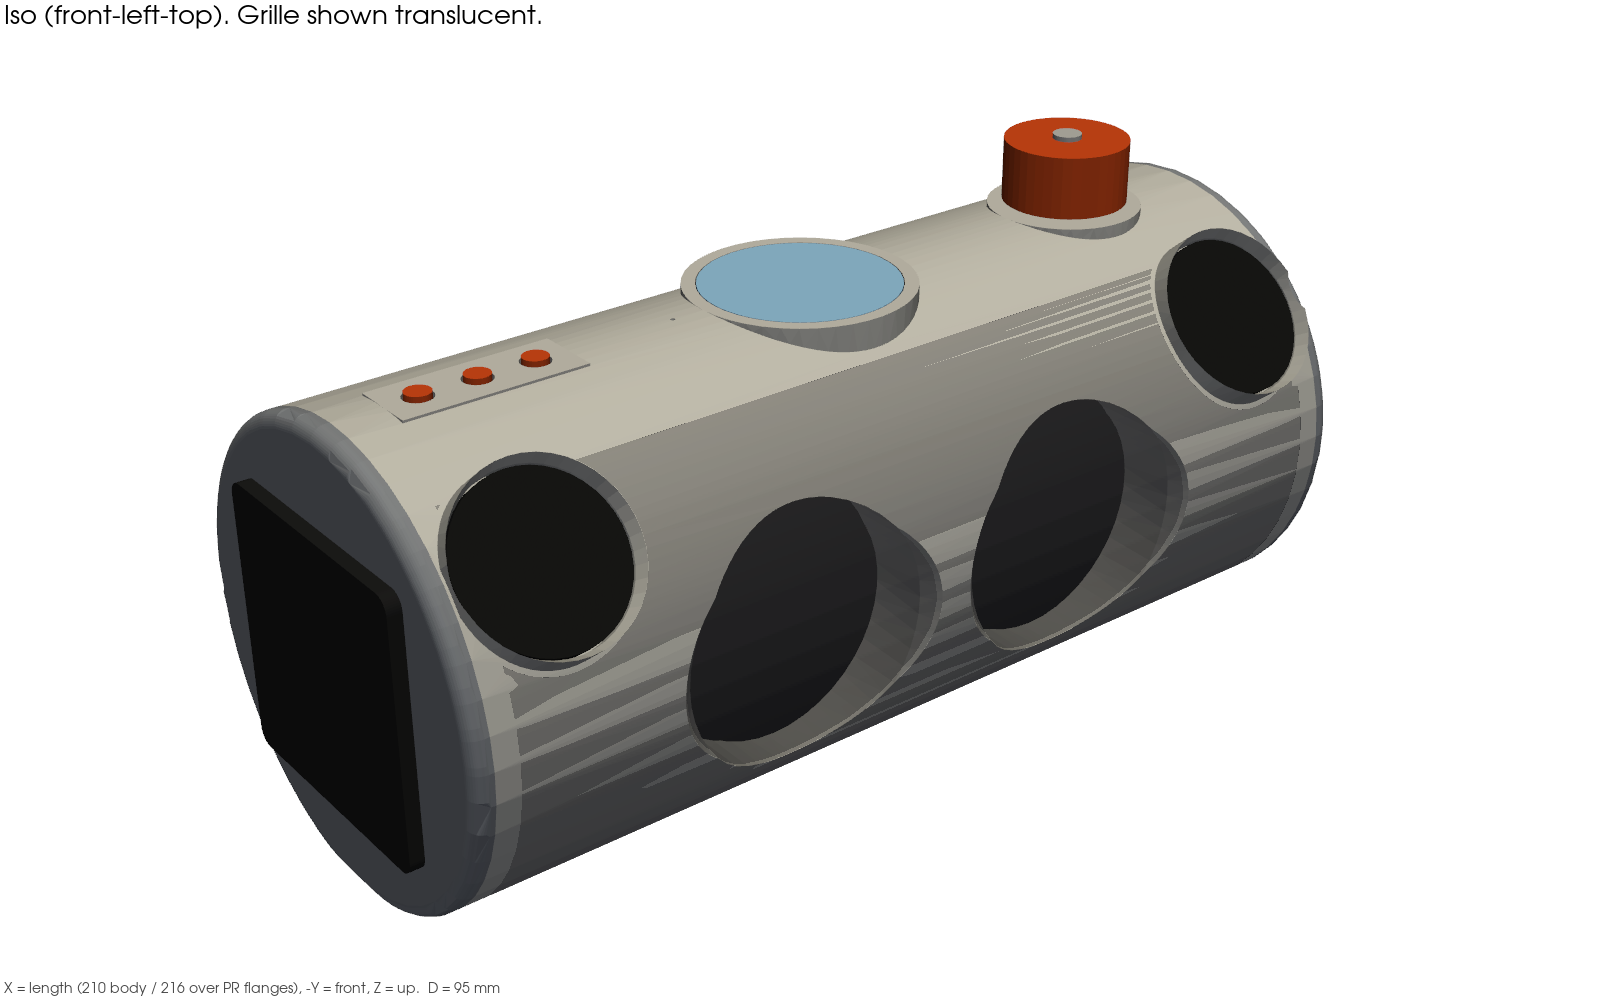
\includegraphics[width=\linewidth]{view_iso.png}
\caption{Iso view: the Ø\qty{95}{\milli\metre} capsule with grille, tweeter bosses on the front shoulders, display and knob on top, and a PR on each end cap.}
\end{subfigure}\hfill
\begin{subfigure}[t]{0.49\linewidth}\centering
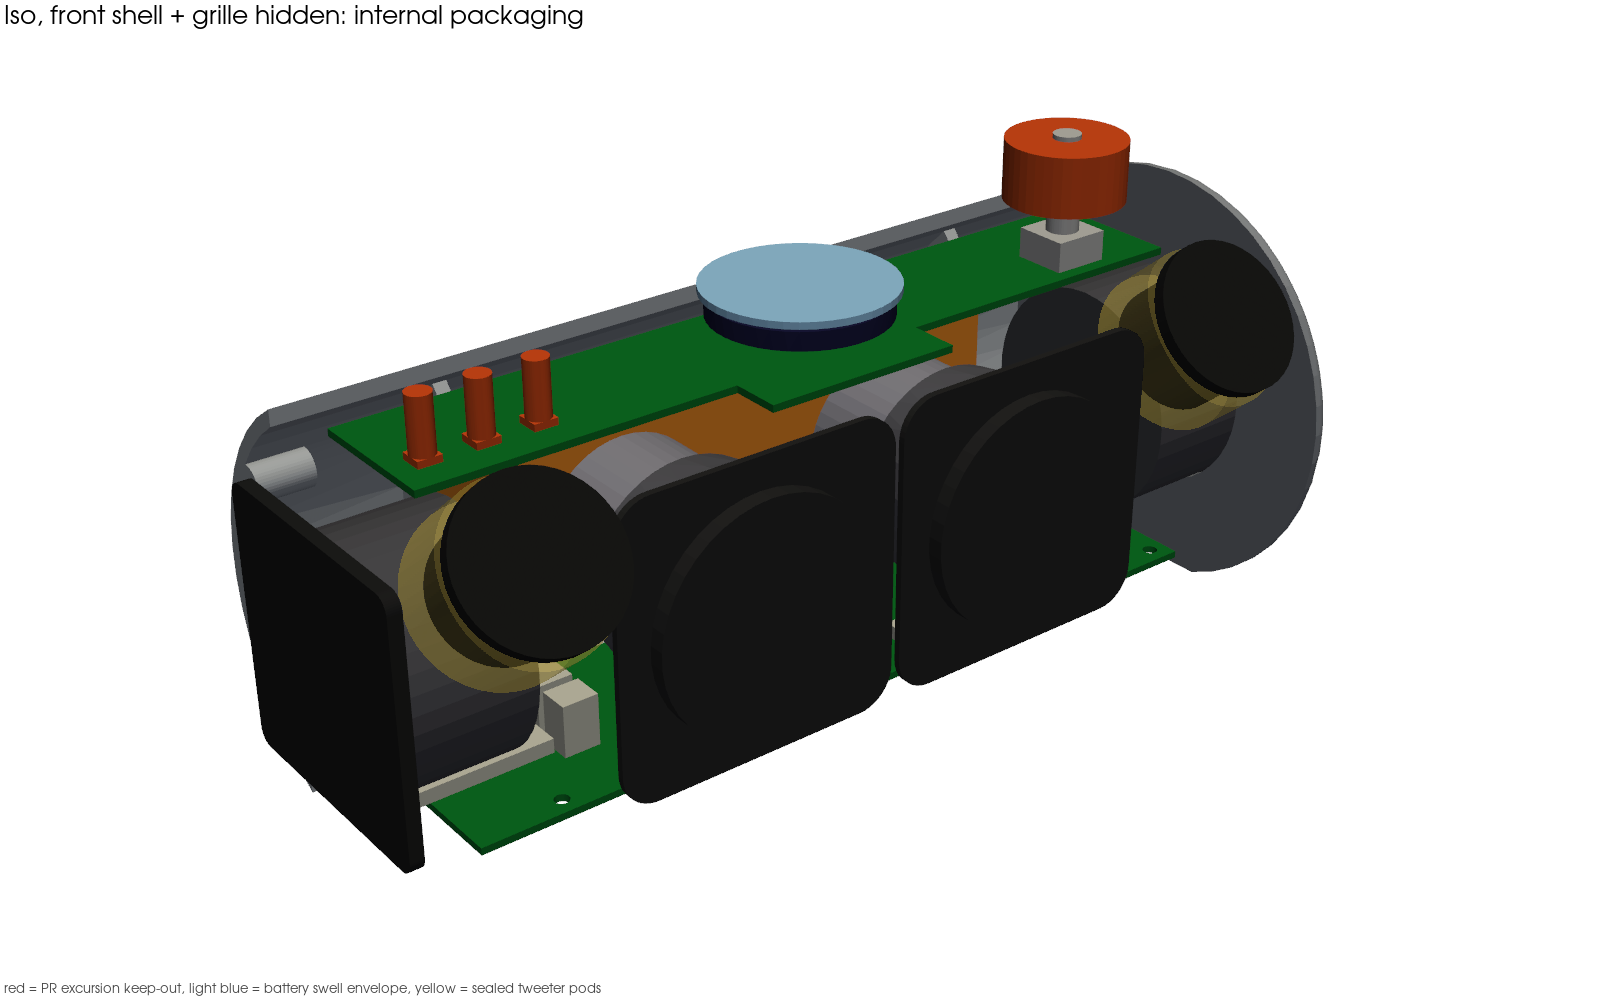
\includegraphics[width=\linewidth]{view_iso_internals.png}
\caption{Front shell and grille hidden: the two woofers rear-mounted \qty{2}{\milli\metre} apart, the UI board under the top, the main board on the floor and the battery behind the woofer motors.}
\end{subfigure}\\[4pt]
\begin{subfigure}[t]{0.49\linewidth}\centering
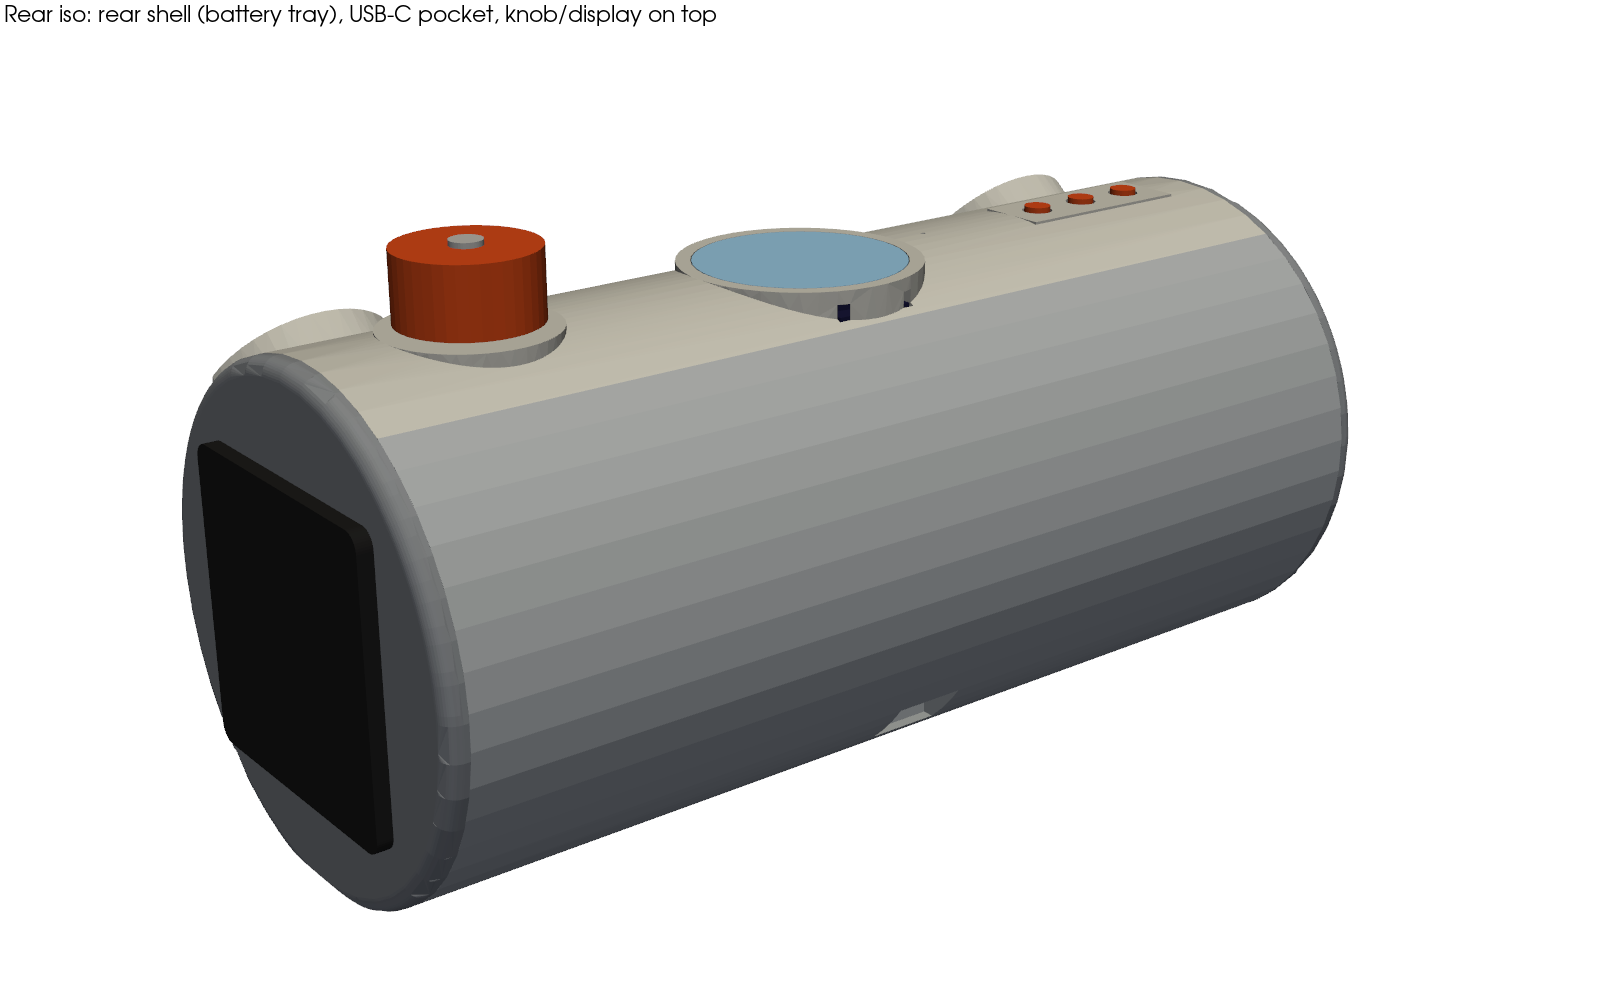
\includegraphics[width=\linewidth]{view_iso_rear.png}
\caption{Rear iso: the shell seam and the USB-C pocket at the bottom centre.}
\end{subfigure}\hfill
\begin{subfigure}[t]{0.49\linewidth}\centering
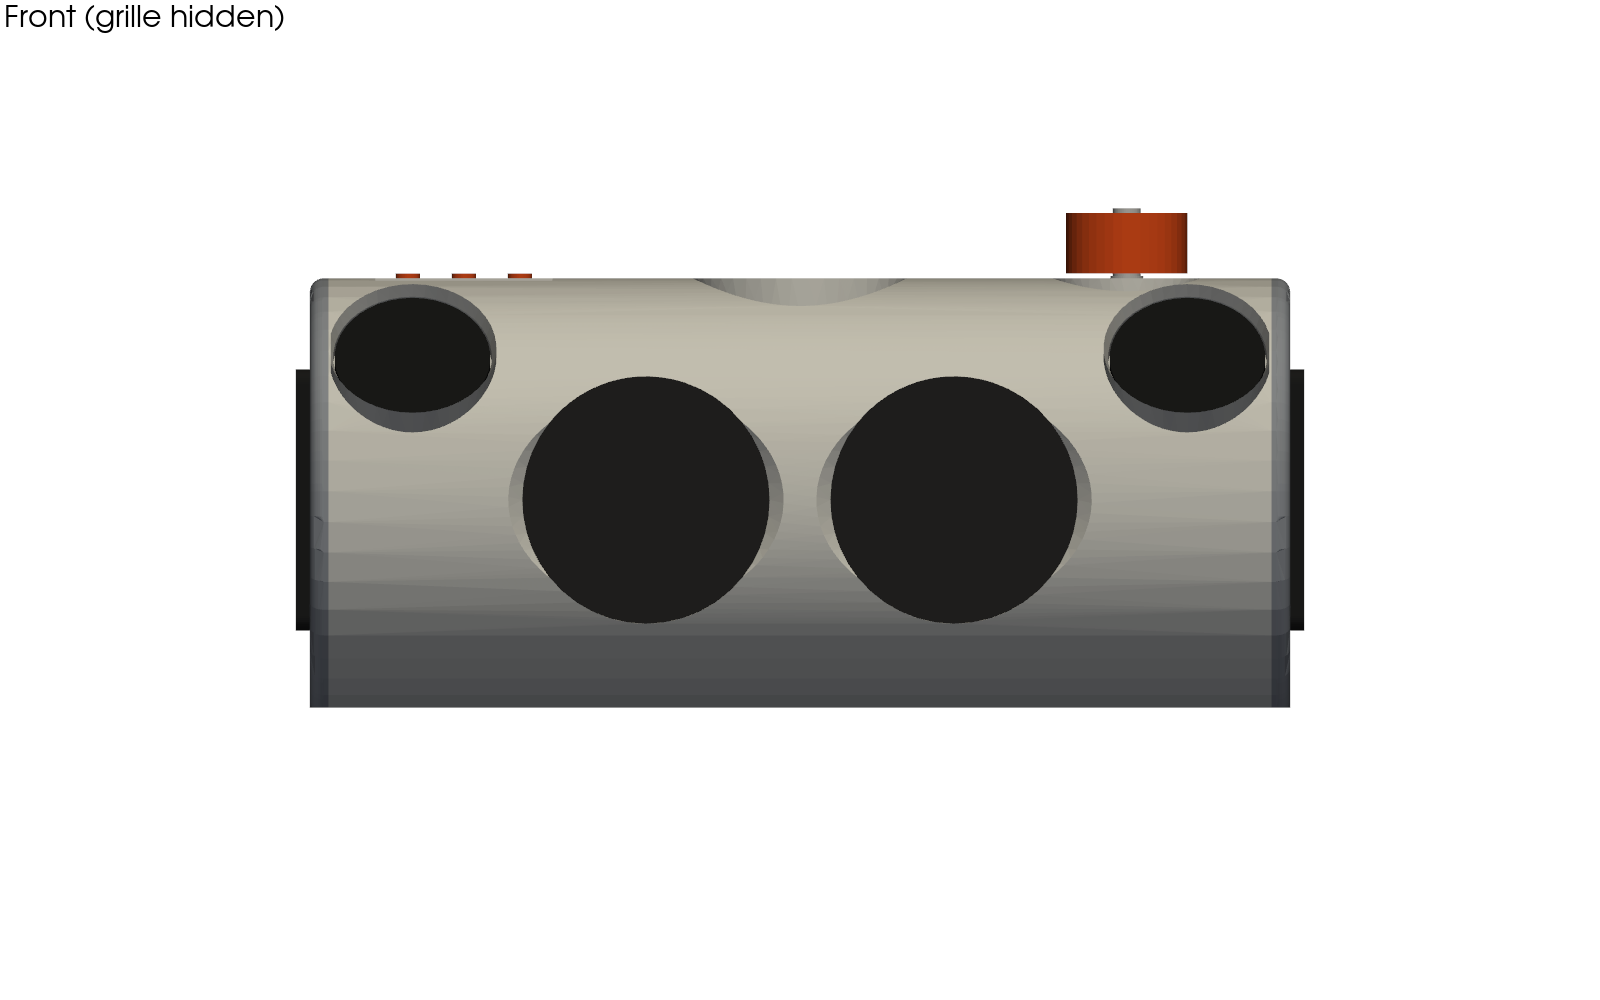
\includegraphics[width=\linewidth]{view_front.png}
\caption{Front: woofer openings \qty{66}{\milli\metre} apart, tweeters \qty{166}{\milli\metre} apart.}
\end{subfigure}
\caption{Concept CAD views. The overall envelope is \qtyproduct{216 x 95 x 92}{\milli\metre}; the knob adds \qty{14}{\milli\metre} on top. In the internal view, red marks the PR excursion keep-outs, light blue the battery swell envelope and yellow the sealed tweeter pods.}
\label{fig:cad-views}
\end{figure}

\begin{figure}[htbp]
\centering
\begin{subfigure}[t]{0.32\linewidth}\centering
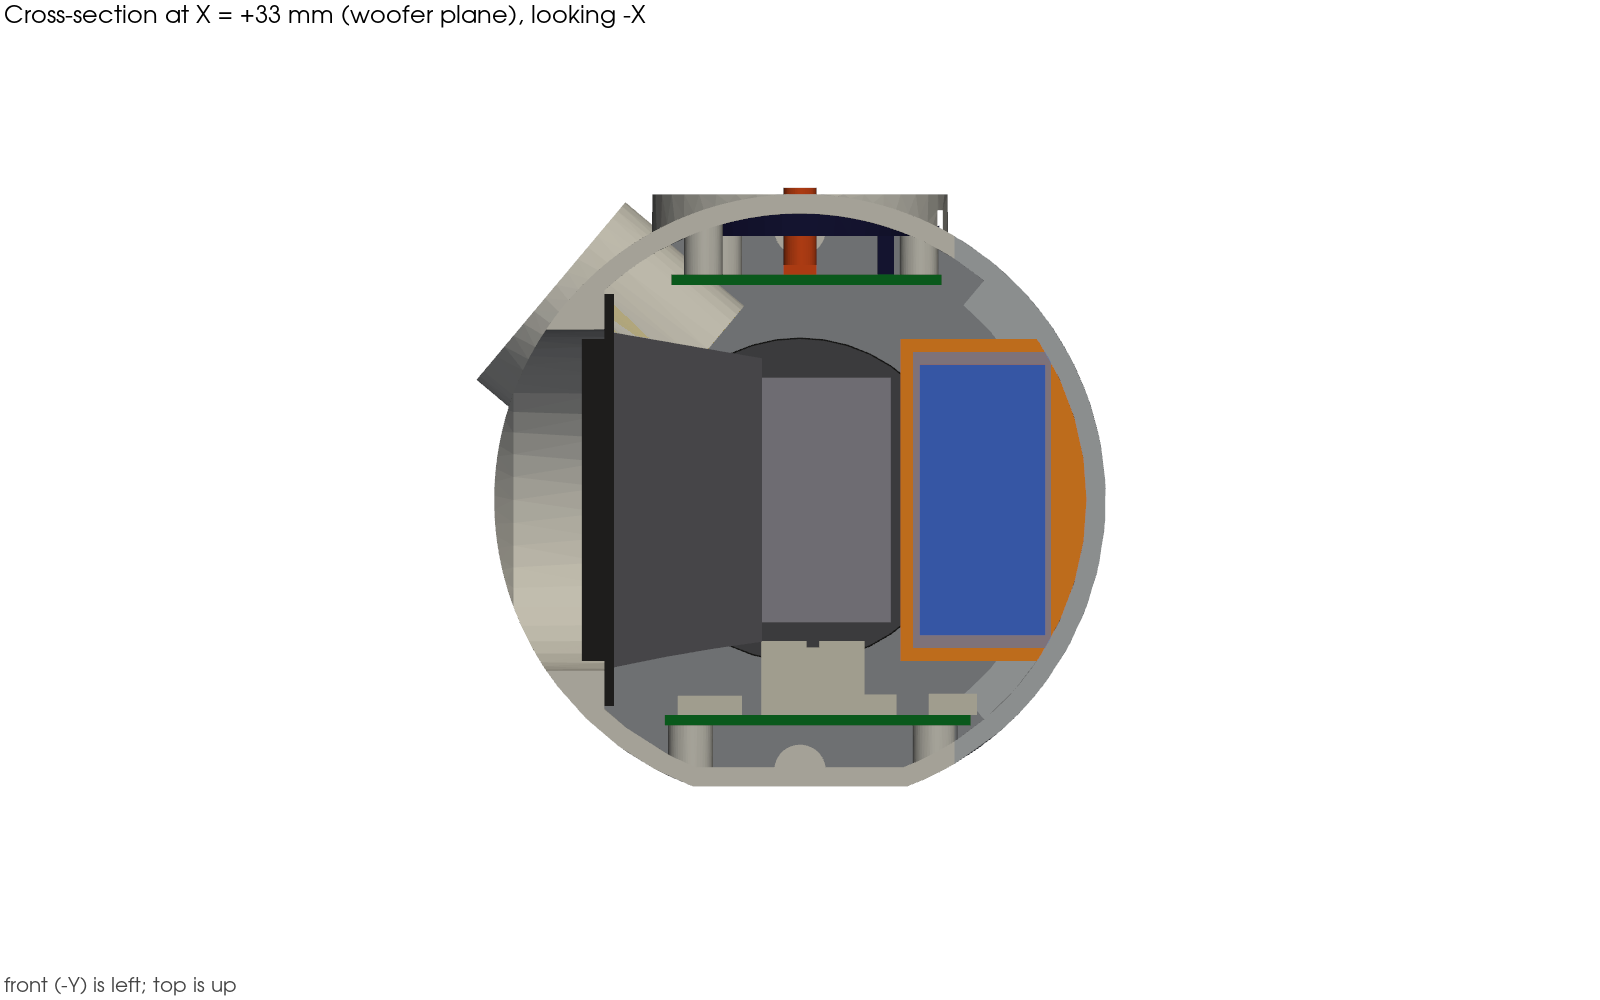
\includegraphics[width=\linewidth]{view_section_xp33_woofer.png}
\caption{Section at $x=\qty{+33}{\milli\metre}$ (woofer).}
\end{subfigure}\hfill
\begin{subfigure}[t]{0.32\linewidth}\centering
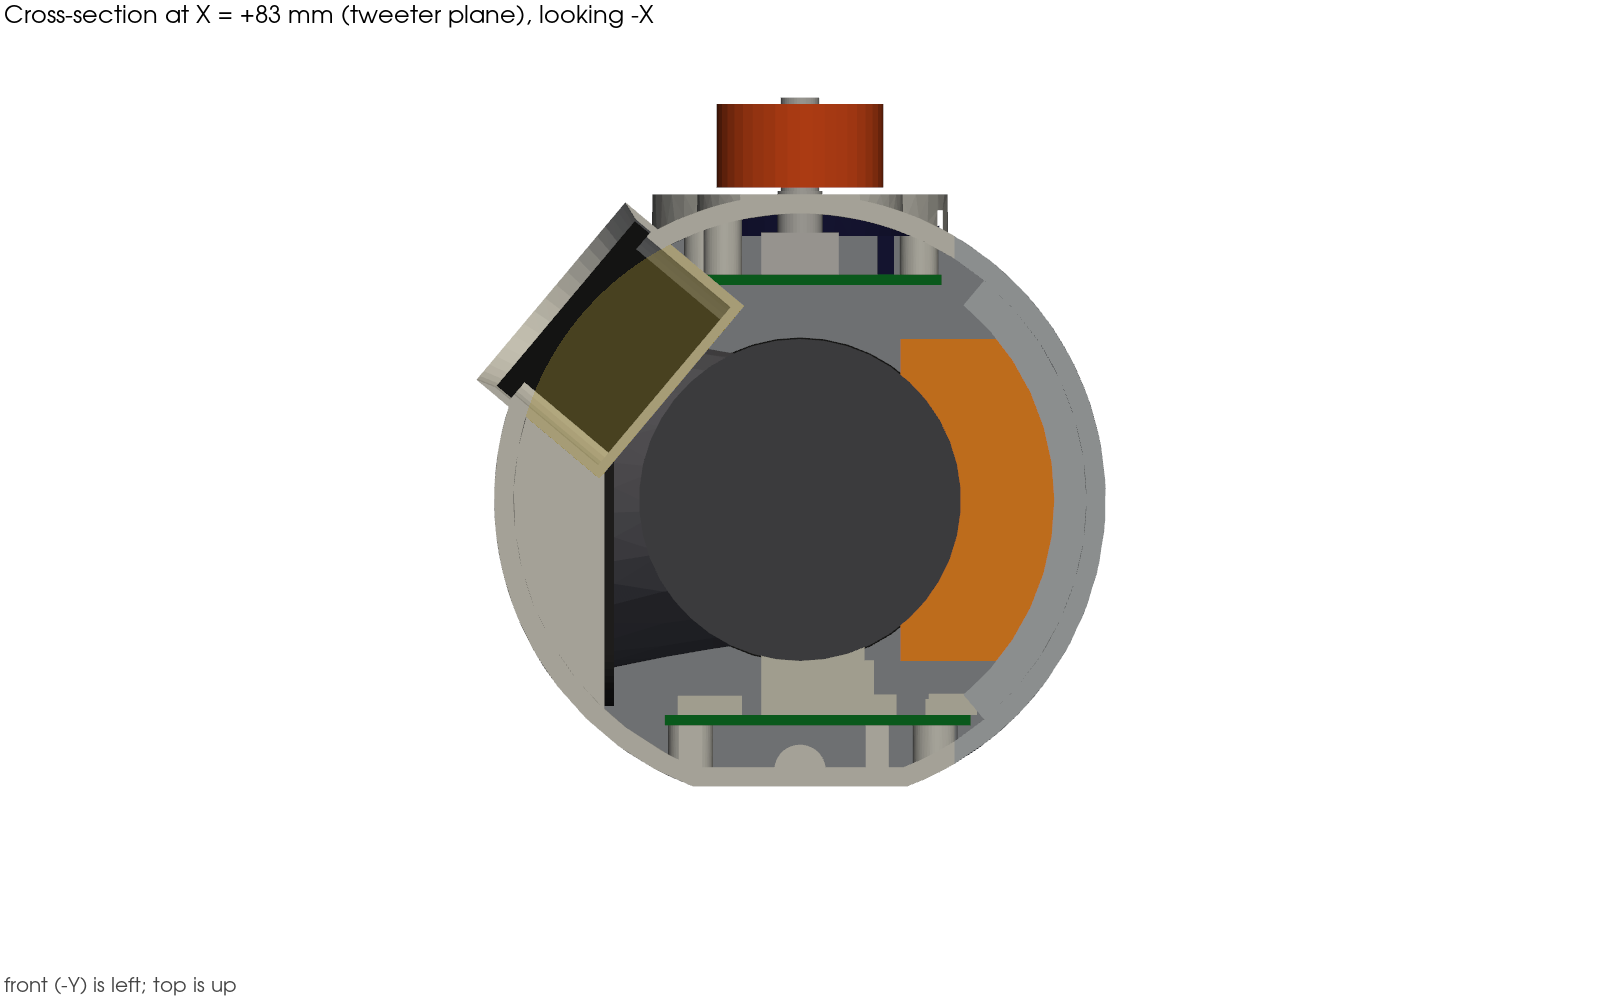
\includegraphics[width=\linewidth]{view_section_xp83_tweeter.png}
\caption{Section at $x=\qty{+83}{\milli\metre}$ (tweeter pod).}
\end{subfigure}\hfill
\begin{subfigure}[t]{0.32\linewidth}\centering
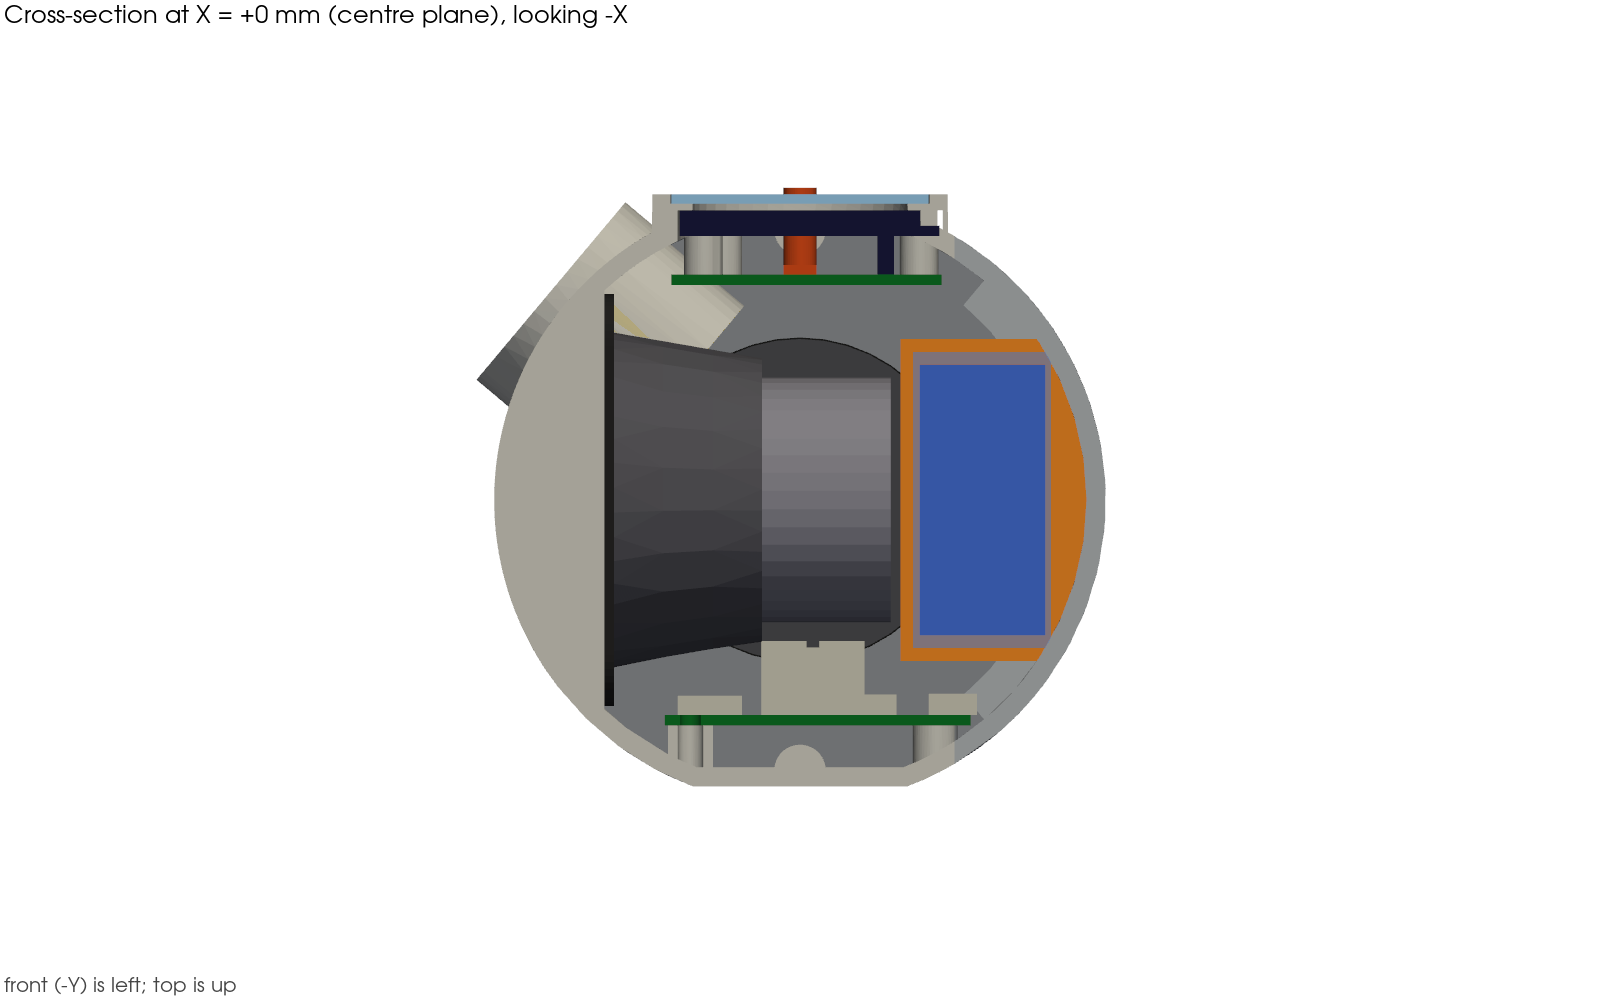
\includegraphics[width=\linewidth]{view_section_xp0_centre.png}
\caption{Section at $x=0$ (centre).}
\end{subfigure}\\[4pt]
\begin{subfigure}[t]{0.49\linewidth}\centering
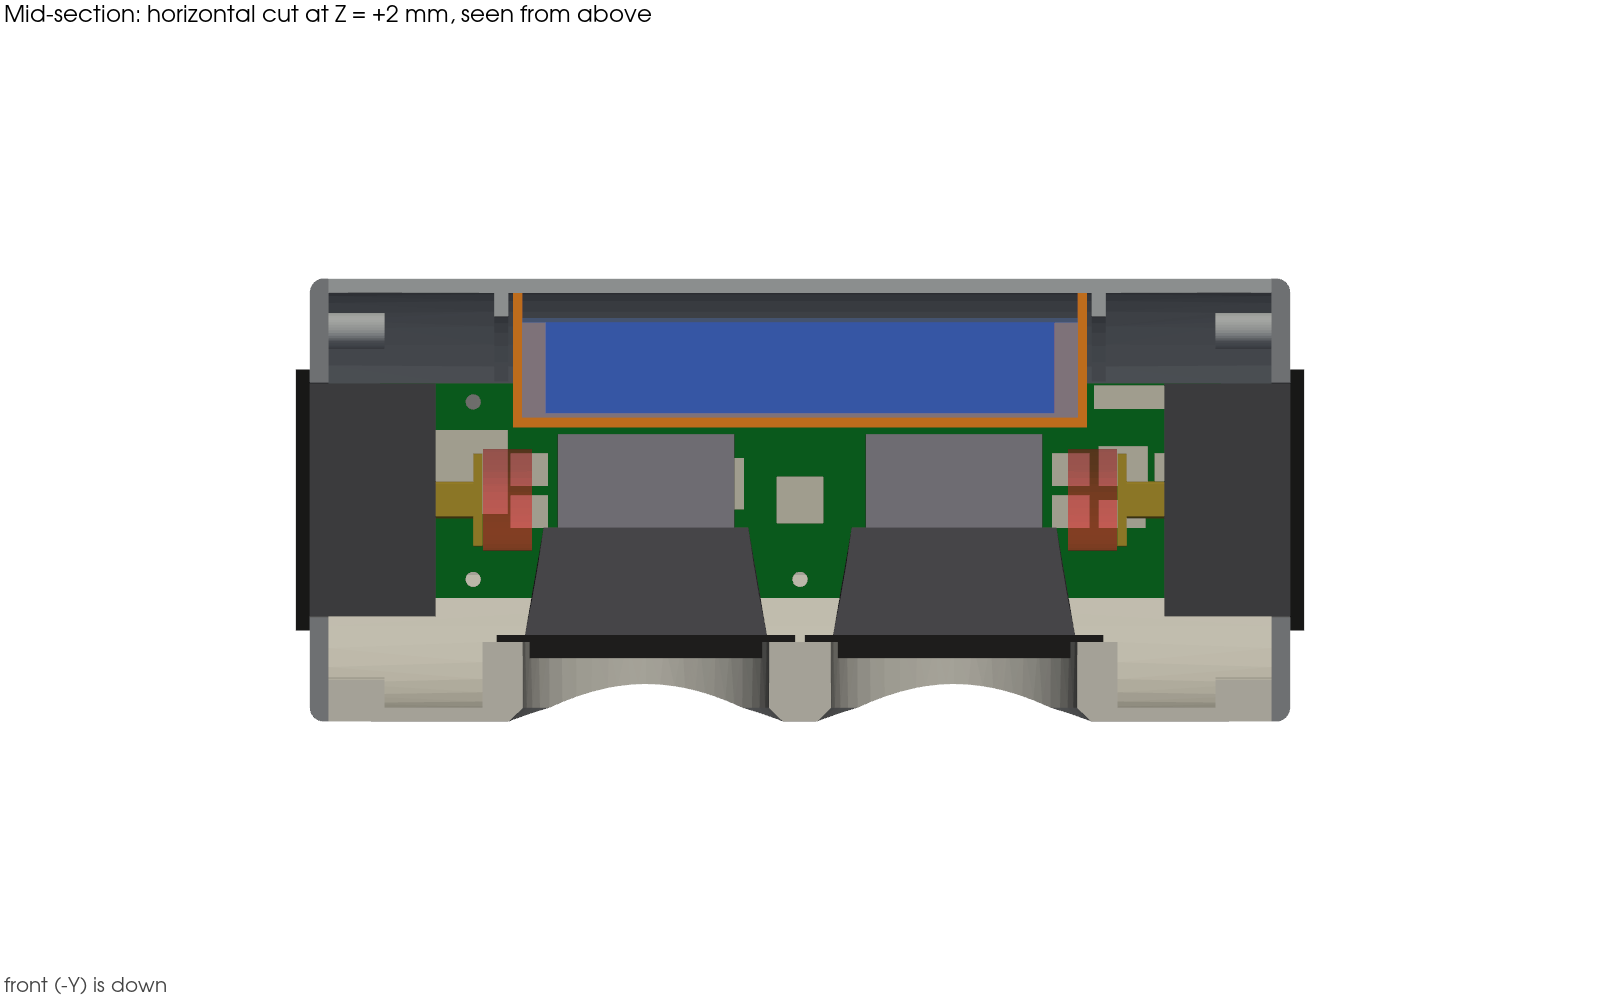
\includegraphics[width=\linewidth]{view_section_z_mid.png}
\caption{Horizontal section at mid-height.}
\end{subfigure}\hfill
\begin{subfigure}[t]{0.49\linewidth}\centering
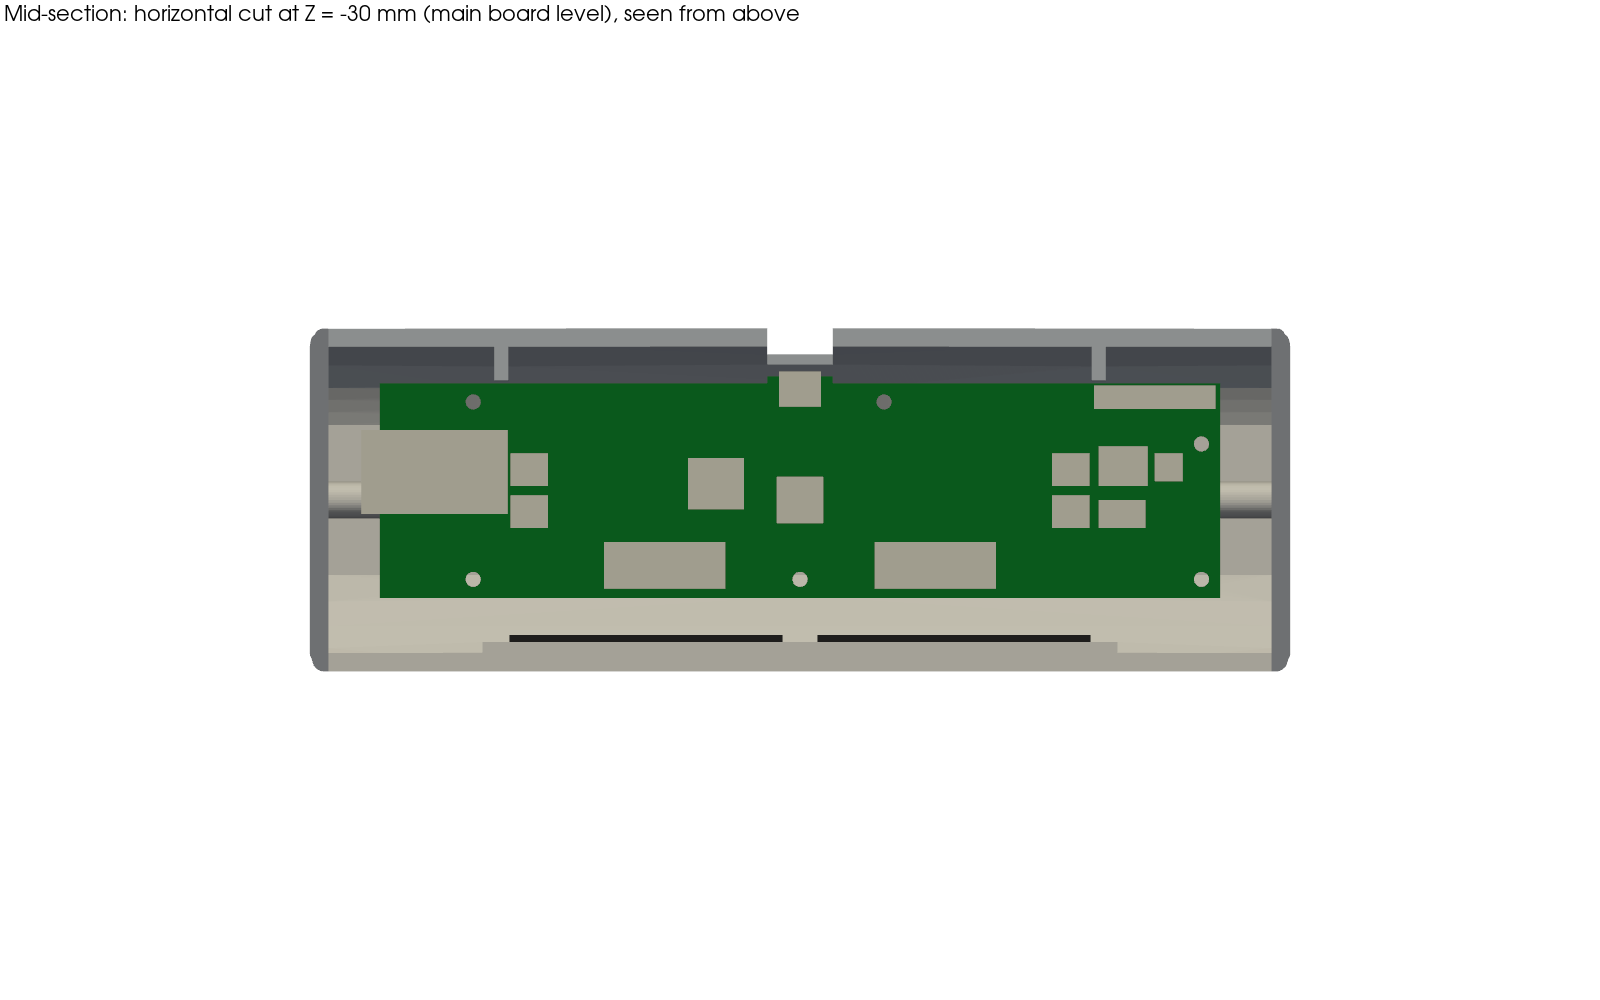
\includegraphics[width=\linewidth]{view_section_z_board.png}
\caption{Horizontal section at the main-board level.}
\end{subfigure}
\caption{Cross-sections. The woofer section shows why the diameter is \qty{95}{\milli\metre}. The ND65-8's flange sits at least \qty{30}{\milli\metre} off the axis, its \qty{48}{\milli\metre} depth eats most of the tube, and the \qty{19.5}{\milli\metre} battery fits only in the slab behind the motors. The tweeter section shows the sealed pod (Ø\qtyproduct{32 x 21.5}{\milli\metre}) squeezed between the PR basket and the skin, which is why the waveguide became a \qty{3}{\milli\metre} bezel.}
\label{fig:cad-sections}
\end{figure}

\subsection{Net volume}

\begin{table}[htbp]
\centering\small
\caption{Net internal volume from the model's solids. Open-frame parts use fill factors: \num{0.25} for the woofer basket and \num{0.2} for the PR basket. Source: \protect\src{docs/mech_envelope.md} §5.}
\label{tab:volume}
\begin{tabular}{@{}l S[table-format=4.1]@{}}
\toprule
Item & {cm\textsuperscript{3}} \\
\midrule
Gross tube interior (Ø89 $\times$ \qty{202}{\milli\metre}, flat floor) & 1243.6 \\
Shell intrusions (baffle land, ribs, bosses, standoffs, pads, tray walls) & -75.8 \\
Tweeter pods (sealed, excluded) & -26.2 \\
Woofer front openings (air outside the box) & -39.3 \\
Woofers $\times$2 & -92.1 \\
PRs $\times$2 (inside portion) & -20.1 \\
Battery (nominal) & -89.3 \\
Main PCB + modelled parts & -21.3 \\
UI PCB, display, encoder, buttons & -14.6 \\
Wiring, foam, gasket allowance & -15.0 \\
\midrule
\textbf{Net box volume} & \bfseries 848 \\
\bottomrule
\end{tabular}
\end{table}

\qty{0.85}{\litre} is \qty{0.10}{\litre} more than the \qty{0.75}{\litre} the driver alignment assumed. Unmodelled board parts and the real driver shapes will cost perhaps another \qtyrange{20}{30}{\centi\metre\cubed}, so A1 uses \qty{0.82}{\litre}. The A1 what-ifs show that the extra volume is worth less than \qty{0.1}{\decibel}, so it is margin, not performance.

\subsection{Part split, fasteners and leaks}

\begin{table}[htbp]
\centering\small
\caption{Printed parts. All fit the \qtyproduct{220 x 220 x 220}{\milli\metre} build volume. The shells print standing on end, so their walls are vertical. Total shell mass is about \qty{310}{\gram} of PETG. Source: \protect\src{docs/mech_envelope.md} §3.}
\label{tab:parts}
\begin{tabularx}{\linewidth}{@{}l l >{\raggedright\arraybackslash}X@{}}
\toprule
Part & Bounding box (mm) & Contents \\
\midrule
Front shell ($y<+24$) & $202\times74\times92$ & Baffle land, tweeter pods, top UI pads and bosses, floor standoffs, seam lips \\
Rear shell ($y>+24$) & $202\times24\,(+8)\times82$ & Battery tray, which doubles as a puncture shield; rear ribs; USB-C pocket \\
End cap $\times2$ & $95\times92\times4$ (+ ribs) & PR mount (flange \qty{3}{\milli\metre} proud), spigot ring with gasket, 5 axial screws \\
Knob, plungers & small & Lens is a laser-cut acrylic or polycarbonate disc \\
Grille (not printed) & \qty{0.8}{\milli\metre} perforated Al & Rolled to $R\,\qty{48.3}{\milli\metre}$; tabs plus VHB; Ø38 holes for the tweeter bosses \\
\bottomrule
\end{tabularx}
\end{table}

The passive-radiator alignment assumes a well-sealed box, so the concept gaskets every seam and driver and seals the encoder, USB-C receptacle, buttons and microphone port. The power button SW4 sits in a recessed Ø\qty{10}{\milli\metre} pocket on the top, so a palm or bag cannot press it \src{docs/mech_envelope.md}.

\begin{checked}
The FreeCAD script checks every pair of solids for interference (none) and reports clearances. The tightest are \qty{0.5}{\milli\metre} (tweeter pod to woofer frame) and \qty{1.0}{\milli\metre} (pod to PR basket, battery to shell). Because they come from datasheet drawings, the real drivers and pack must be measured and the script re-run. The net volume is computed from the solids, with fill factors for open-frame parts. The same parameter block drives the BEM hull, whose sections match the CAD within a median of \qtyrange{0.7}{0.9}{\milli\metre}.
\end{checked}

\subsection{PCB envelopes}

\begin{figure}[htbp]
\centering
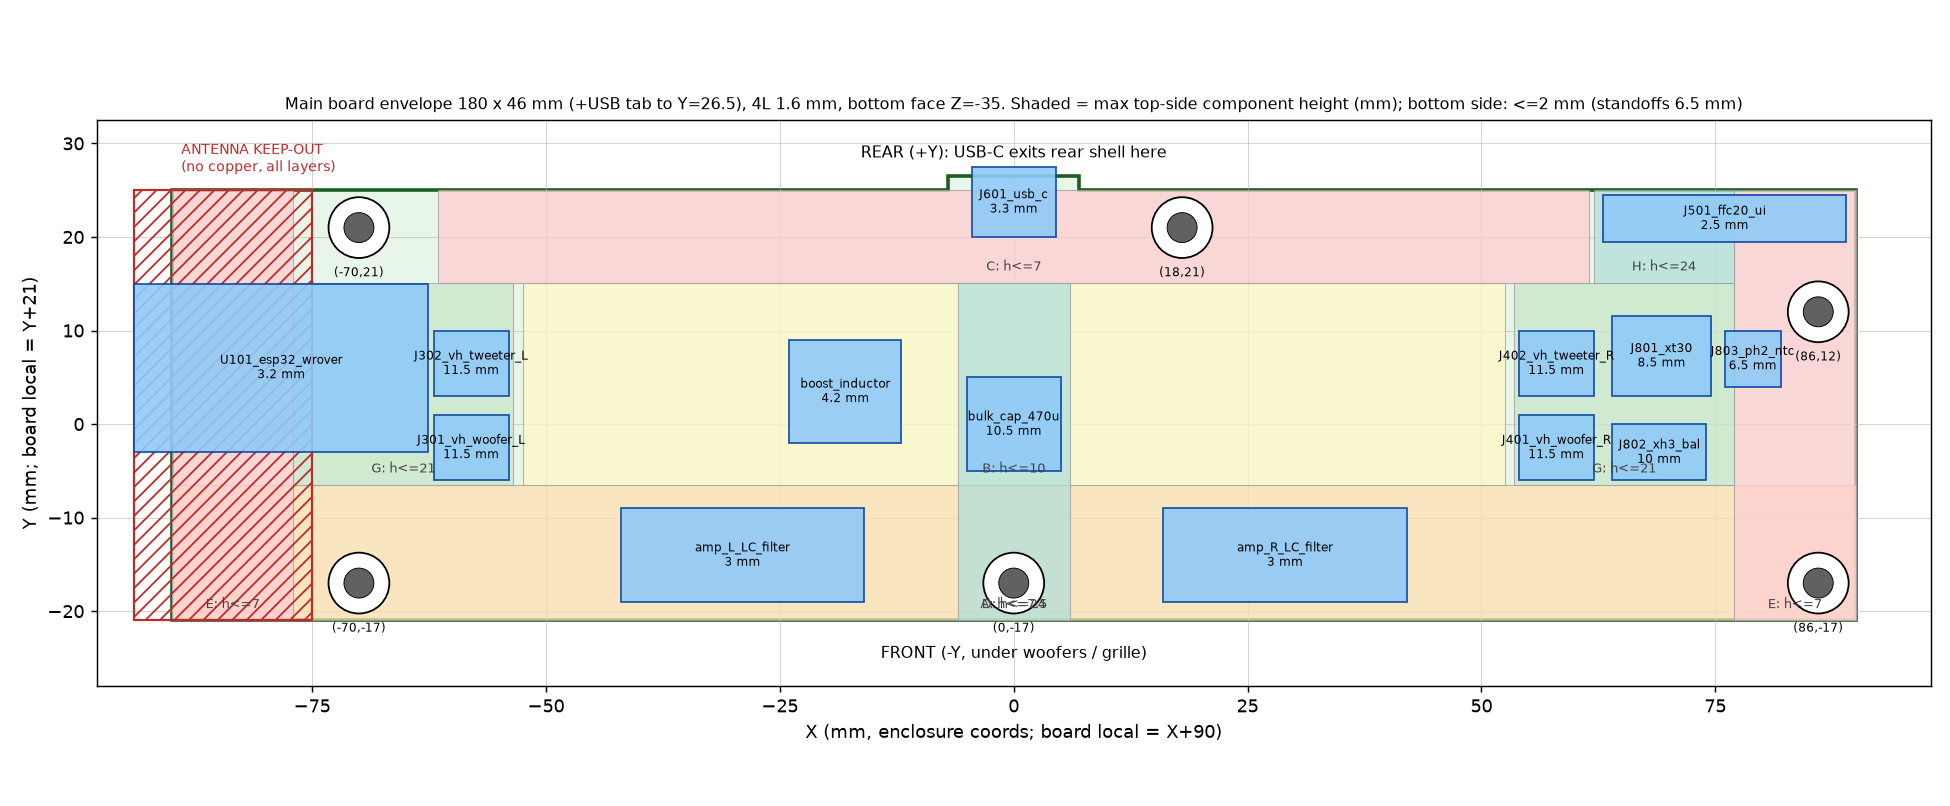
\includegraphics[width=\linewidth]{mainboard_envelope.png}
\caption{Main-board envelope: \qtyproduct{180 x 46}{\milli\metre} plus a USB-C tab, 4 layers, six M3 holes. Each height zone is set by what sits above it: \qty{7.5}{\milli\metre} under the woofer baskets, \qty{10}{\milli\metre} under the motors, \qty{24}{\milli\metre} in the centre for the \qty{470}{\micro\farad} capacitor, \qty{21}{\milli\metre} between motor and PR for the connectors. The ESP32 antenna overhangs the $-x$ edge, with no copper on any layer for $x<\qty{-75}{\milli\metre}$.}
\label{fig:mainboard-env}
\end{figure}

\begin{figure}[htbp]
\centering
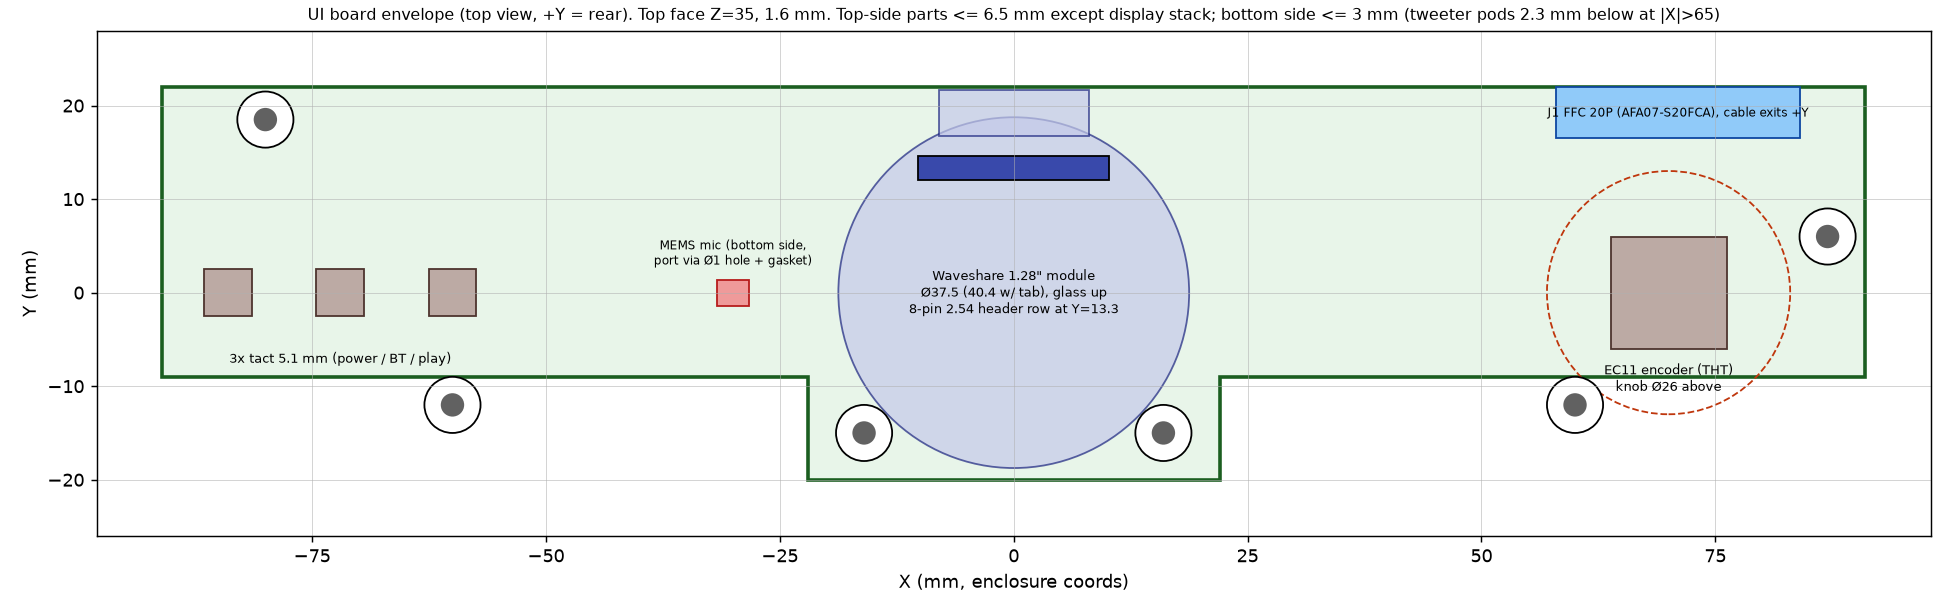
\includegraphics[width=\linewidth]{uiboard_envelope.png}
\caption{UI-board envelope: \qtyproduct{182 x 31}{\milli\metre} with a paddle under the display. It holds the display at $x=0$, the encoder at $x=\qty{+70}{\milli\metre}$, three buttons at $x=-60/-72/\qty{-84}{\milli\metre}$, the bottom-port microphone at $x=\qty{-30}{\milli\metre}$, and the FFC connector at the rear-right. The FFC runs about \qty{90}{\milli\metre} down the inside wall to J501.}
\label{fig:uiboard-env}
\end{figure}

\section{Schematic}\label{sec:schematic}

The main board was drawn in KiCad 10.0.4 entirely through the Konnect MCP server. No agent edited a KiCad file as text. The current release, \textbf{v0.2}, includes the readability redraw, a root block diagram with sheet pins, ECO-001 and ECO-002 \src{hw/mainboard/BUILD_NOTES.md}. It has 271 parts on nine sheets (\cref{tab:sheets}); 12 of them are DNP. \Cref{fig:sch-root,fig:sch-rails,fig:sch-mcu,fig:sch-amp} reproduce four pages. The full PDF is \repo{hw/mainboard/out/speaker_main_schematic.pdf}.

\begin{checked}
\begin{itemize}[leftmargin=1.2em,itemsep=1pt]
  \item \textbf{Against the spec:} RefDes coverage was checked by script, and every IC, transistor and connector was checked pin by pin using the nets read back from KiCad.
  \item \textbf{ERC:} 0 violations at all severities, no exclusions. One caveat: the CH340C symbol hides +3V3's real driver, so that net was confirmed in the netlist.
  \item \textbf{After every edit} (redraw, root rework, ECO-001, ECO-002), the netlist was compared with the previous release. Only the intended changes appeared.
  \item \textbf{Reviews:} an independent review and two skill-driven release reviews, v0.1 and the v0.2 delta. They covered pins against pads, footprints against drawings, boundary states and supply. Verdict: \textbf{no blockers}; the open items are in \cref{app:register}.
\end{itemize}
\end{checked}

\textbf{Still to do before fabrication:}
\begin{itemize}
  \item Set KiCad's DNP attribute on the 12 parts; Konnect cannot set it.
  \item Confirm the XT30 polarity on a real part.
  \item Plan placement of the three tall electrolytics.
  \item Fix the small documentation leftovers in \cref{sec:inconsistencies}.
\end{itemize}

\newcommand{\schpage}[3]{%
\begin{figure}[p]
\centering
\includegraphics[page=#1,angle=90,width=0.97\linewidth,height=0.86\textheight,keepaspectratio]{speaker_main_schematic.pdf}
\caption{#2}\label{#3}
\end{figure}}

\schpage{1}{Schematic v0.2, root sheet: the KiCad version of \cref{fig:power-path,fig:data-path}. The power path runs along the top (USB, charger, battery, rails, amplifiers); the data path runs below (USB-UART, MCU, UI link, amplifiers). The blue bus carries I\textsuperscript{2}C, AMP\_PDN, the fault lines, I\textsuperscript{2}S and CHG\_QON.}{fig:sch-root}

\schpage{5}{Page 5, \texttt{rails}. Top: the TPS61178 boost with the ECO-001 compensation (\qty{100}{\kilo\ohm}/\qty{15}{\nano\farad}) and the trim network R907/D901, now fitted for the soft start. Bottom: the TPS62933 buck to +3V3. The text blocks are the design notes the build agent placed on each sheet.}{fig:sch-rails}

\schpage{6}{Page 6, \texttt{mcu}. The ESP32-WROVER-E with every usable GPIO assigned, the I\textsuperscript{2}C pull-ups, the \qty{2.2}{\micro\farad} EN capacitor, the \qty{68}{\ohm} SPI/PDM source resistors, the two-FET fault merge and test points TP105--TP110.}{fig:sch-mcu}

\schpage{9}{Page 9, \texttt{amp\_left}. The TAS5805M in BTL with its address strap (0x2C), PVDD decoupling, bootstrap capacitors and the four \qty{10}{\micro\henry} + \qty{1}{\micro\farad} output legs to the woofer (channel A) and tweeter (channel B). The right amplifier (page 10) differs only in RefDes, strap and test points.}{fig:sch-amp}

\clearpage

\section{PCB layout (pending)}\label{sec:layout}

This chapter will be filled in after layout. The inputs are ready:
\begin{itemize}
  \item the board envelopes and height zones (\cref{fig:mainboard-env,fig:uiboard-env});
  \item the layout checklists in both specs;
  \item the release reviews' placement conditions (tall capacitors, XT30 polarity, AGND/PGND tie);
  \item the project's layout principles, \repo{docs/layout_principles.md}.
\end{itemize}
The principles say that layout is where LLMs are weakest, so the board will be judged by physics, not just by connectivity and DRC:
\begin{itemize}
  \item The model writes net classes and rules from the datasheets' layout sections, with page citations.
  \item An autorouter handles non-critical nets.
  \item Power stages, switch nodes, the USB pair and high-current paths are routed deliberately and reviewed.
  \item The result is scored with loop-inductance, PDN and IR-drop checks. Post-layout parasitics go back into the S7 PDN model.
\end{itemize}

\begin{figure}[htbp]
\centering
\begin{subfigure}[t]{0.49\linewidth}\centering\pendingbox[0.95\linewidth]{4.5cm}\caption{Main board: placement and top copper.}\end{subfigure}\hfill
\begin{subfigure}[t]{0.49\linewidth}\centering\pendingbox[0.95\linewidth]{4.5cm}\caption{Main board: 3D view in the enclosure envelope.}\end{subfigure}
\caption{PCB layout: placeholders until the layout exists.}
\label{fig:layout-pending}
\end{figure}

\section{Still to come}\label{sec:pending}

\begin{enumerate}
  \item \textbf{Thermal simulation.} A Python finite-difference solver on the real copper, cross-checked in CalculiX. Inputs: boost \qtyrange{0.5}{2.5}{\watt}, amplifiers 1--\qty{3}{\watt} each when loud, charger \qty{1.5}{\watt}, battery path \qty{1}{\watt}, and Q801 \qty{1.5}{\watt} during deep-discharge recovery. All of it sits in a sealed box \src{research/electronics.md}.
  \item \textbf{Post-layout PDN:} replace the placeholder copper in the S7 model with extracted values.
  \item \textbf{Enclosure detail:} the spine plate, damping pads and battery clamp from A4; optional tilt feet against the desk dip from A2.
  \item \textbf{Renders:} Blender renders of the assembled speaker.
  \item \textbf{Build and measure.}
  \begin{itemize}
    \item Measure the drivers' T/S parameters and re-run A1.
    \item Run the bench list (\cref{sec:bench}).
    \item Measure SPL, $F_3$ and polar response with REW and a UMIK-1 against the A1/A5 predictions, and refine the A5 EQ.
  \end{itemize}
  \item \textbf{Firmware:} ESP-IDF, built to the contract in \cref{sec:firmware-req}.
\end{enumerate}

\begin{figure}[htbp]
\centering
\begin{subfigure}[t]{0.32\linewidth}\centering\pendingbox[0.95\linewidth]{3.5cm}\caption{Blender render.}\end{subfigure}\hfill
\begin{subfigure}[t]{0.32\linewidth}\centering\pendingbox[0.95\linewidth]{3.5cm}\caption{Thermal map at \qty{40}{\watt}, \qty{6}{\volt} battery.}\end{subfigure}\hfill
\begin{subfigure}[t]{0.32\linewidth}\centering\pendingbox[0.95\linewidth]{3.5cm}\caption{Measured SPL against the A5 prediction.}\end{subfigure}
\caption{Placeholders for results that do not exist yet.}
\label{fig:pending}
\end{figure}

\section{What I'd change in v2}\label{sec:v2}

These are recommendations drawn from the findings above, not decisions.

\subsection{Hardware}
\begin{itemize}
  \item \textbf{Design the boost loop and the bulk capacitance together.} With \qty{1.5}{\milli\farad} on PVDD, the loop, not the capacitors, sets the bass-band impedance, and that impedance should be a requirement from the start. It took a simulation to see this (S1, S7).
  \item \textbf{A soft start by design.} Fit the trim network by default, or choose a boost converter with an external soft-start pin, so PVDD never winds up past \qty{18}{\volt} (S1).
  \item \textbf{Protection that does not depend on firmware.} The fast PVDD short protection is a charger register that a watchdog expiry clears (review S1). A v2 should restore a hardware path: a disconnect FET sized for the bulk, a smaller fuse, or a protector with a lower over-current threshold.
  \item \textbf{Detect a missing balance lead and an over-temperature pack in hardware.} With the balance lead out, the mid-tap bias hides cell-level faults (S7), and nothing in hardware stops \emph{discharge} when the pack is hot (S6). Neither has a spare ADC or GPIO today.
  \item \textbf{A low-capacitance I\textsuperscript{2}C isolator,} so the bus can run at \qty{400}{\kilo\hertz} without scoping first (S5).
  \item \textbf{GPIO headroom.} The WROVER-E leaves no spare pin: no PVDD sense, no I2S\_SEL read-back, no JTAG. An I\textsuperscript{2}C GPIO expander for the slow signals would free several pins.
  \item \textbf{Sample-locked microphone.} The firmware research recommends running the microphone on the same I\textsuperscript{2}S peripheral as the amplifiers, so capture is sample-locked to playback. The hardware put the PDM mic on I\textsuperscript{2}S0 and the amplifiers on I\textsuperscript{2}S1, because PDM RX exists only on I\textsuperscript{2}S0. Either move the amplifiers to I\textsuperscript{2}S0 as well, or confirm that the two peripherals can share a clock source.
  \item \textbf{Cable.} Put a ground between MOSI and CS on the FFC (S6). The \qty{68}{\ohm} source resistors and the \qty{100}{\milli\metre} cable are already in v0.2.
  \item \textbf{A battery that matches the requirement.} A custom device-grade 2S pouch with a pack NTC and a rated continuous current (the BatterySpace quote route) needs a \qty{50}{\milli\metre}-wide bay. The on-board TH801 measures board temperature, not cell temperature (S3).
  \item \textbf{Enclosure.} Add the centre spine plate and damping pads (A4). Keep \qty{10}{\milli\metre} in the length budget for a real tweeter waveguide if A2 shows it is worth it.
  \item \textbf{More bass headroom.} The system is limited by amplifier voltage. The only cheap lever is the woofer limiter (\qty{+0.9}{\decibel} at \qty{17.1}{\volt}); the next one is a \qty{6}{\ohm} woofer, worth about \qty{1}{\decibel} if a suitable one appears.
\end{itemize}

\subsection{Process}
\begin{itemize}
  \item \textbf{A decision log next to the requirements file.} One line per decision, with an owner, a version and a date. Agents cite the version they built against (playbook R3).
  \item \textbf{A consistency check before each phase.} Ask one agent to diff all specs against the requirements and list the conflicts. The first edition of this report found thirteen; after ECO-002 ten remain (\cref{sec:inconsistencies}).
  \item \textbf{Pilot-first by default} for any task that fans out to sub-agents (R4).
  \item \textbf{A compute scheduler.} One heavy simulation at a time, with a disk-space guard (R11).
  \item \textbf{Run the circuit simulations before the schematic is drawn.} ECO-001 changed values the schematic agent had just placed; running S1--S7 straight from the specs would have saved a round.
\end{itemize}


\clearpage
\appendix
\setcounter{secnumdepth}{1}
\addtocontents{toc}{\protect\setcounter{tocdepth}{1}}
% Appendices. The spec appendices are generated by convert_sources.py (pandoc).

\section{Requirements (as of this build)}\label{app:requirements}
{\small Converted with pandoc from \texttt{docs/requirements.md}. Remaining conflicts with other documents are listed in \cref{sec:inconsistencies}.\par}
\begingroup\small
% GENERATED by convert_sources.py from docs/requirements.md. Do not edit by hand.
\subsection{Portable Stereo Bluetooth Speaker --- Requirements (v0.1)}

Working name: \textbf{TBD}. Goal: a ``vibe hardware'' mixed-signal project (digital + analog + power) that holds its own against a JBL Flip/Charge-class speaker, built from a JLCPCB-assembled PCB, LCSC parts, 3D-printed enclosure (Flashforge Adventurer 5M Pro), and off-the-shelf drivers/hardware.

\subsubsection{1. Product targets}

{\def\LTcaptype{none} % do not increment counter
\begin{longtable}[]{@{}
  >{\raggedright\arraybackslash}p{(\linewidth - 4\tabcolsep) * \real{0.3333}}
  >{\raggedright\arraybackslash}p{(\linewidth - 4\tabcolsep) * \real{0.3333}}
  >{\raggedright\arraybackslash}p{(\linewidth - 4\tabcolsep) * \real{0.3333}}@{}}
\toprule\noalign{}
\begin{minipage}[b]{\linewidth}\raggedright
Item
\end{minipage} & \begin{minipage}[b]{\linewidth}\raggedright
Target
\end{minipage} & \begin{minipage}[b]{\linewidth}\raggedright
Notes
\end{minipage} \\
\midrule\noalign{}
\endhead
\bottomrule\noalign{}
\endlastfoot
Channels & Stereo, 2-way per side, \textbf{bi-amped} (active DSP crossover) & 4 driver channels total \\
Drivers & 2× woofer (2.5--3.5''), 2× tweeter (\textasciitilde¾''), 2× passive radiator & PRs on end caps (visible) \\
Bass extension & F3 ≤ 65 Hz (with DSP), F6 ≤ 55 Hz & JBL Flip 6 ≈ 63 Hz \\
Max SPL & ≥ 90 dB @ 1 m (pink noise, battery, \textbf{on a table / half-space}) & limiter-protected; free-air ≈ 85 dB \\
Driver layout & Woofers rear-mounted on front face (66 mm apart); \textbf{tweeters angled up 40° in sealed printed pods} on the front shoulders (166 mm apart), \textbf{minimal 3 mm bezel instead of a full waveguide (decided; verify with BEM sim)} & see \texttt{docs/\allowbreak{}mech\_\allowbreak{}envelope.md} \\
Enclosure (decided) & \textbf{Ø95 × 210 mm body, 216 mm over PR flanges}, 5 printed PETG parts, \textasciitilde0.85 L net & nothing in stock fits Ø90 \\
Battery pick (decided) & \textbf{Gens ace 2S 5000 mAh TX/RX LiPo} (109×42×19.5 mm, \textasciitilde\$31), bonded 10 k NTC; fallback Gens ace 3500 mAh with spacer & RC-brand, no PCM: board protection covers it; bench-test 6 A \\
Amp power & \textasciitilde15--20 W/woofer, \textasciitilde5--10 W/tweeter & boost rail \textasciitilde18--20 V \\
Source & Bluetooth A2DP sink (SBC required, AAC nice-to-have) & \\
Control & Wi-Fi web UI for live EQ/presets; rotary encoder + push; 2--3 buttons & \\
Display & 1.28'' round TFT (GC9A01-class) on top & mode, EQ curve, level meter, battery \\
Mic & 1× digital MEMS mic & placement (bass) compensation + ambient auto-loudness \\
Battery & Off-the-shelf \textbf{pre-built 2S pack} (no spot welding), plugs in via \textbf{XT30 (power) + JST-XH 3-pin (balance)}; charger/balancing/protection stay on our board. Pouch pack preferred; \textbf{no device-grade pack fits the capsule, so the decided pack is the Gens ace 2S 5000 mAh TX/RX LiPo} (see Battery pick row); enclosure needs swell clearance + puncture protection; charge current ≤ 0.5C unless the pack datasheet says otherwise & JLC won't ship cells; ≤ \textasciitilde40 W avg draw (charger BATFET 6 A RMS) \\
Drivers (\textbf{set B8, decided}) & 2× Dayton ND65-8 woofer (8 Ω), 2× Peerless OT19NC00-04 tweeter (4 Ω), 2× Dayton DMA58-PR & \$93.54 at Parts Express; F3 64 Hz, \textasciitilde90.6 dB pink (half-space, A1 refined model), ≥0.50 L net; see \texttt{research/\allowbreak{}drivers.md} \\
Amp rail & \textbf{PVDD 18 V} (TPS61178), DNP trim for dynamic PVDD & 8 Ω woofers keep the TAS5805M well under its 5 A OCP \\
Runtime & ≥ 8 h at moderate volume & \\
USB & USB-C: PD sink charging/power, play-while-charging, firmware flashing & USB-audio input = \textbf{optional add-on, decide after research} \\
Size & Horizontal capsule, ≤ \textasciitilde210 mm long, \textasciitilde80--95 mm dia & printer volume 220×220×220 mm \\
Budget & \textasciitilde\$250 for v1 (5 PCBA, drivers, filament, hardware, UMIK-1 mic) & \\
\end{longtable}
}

Out of scope: waterproofing, multi-speaker linking, phone app (web UI instead), LDAC/aptX.

\subsubsection{2. Block diagram}

{\scriptsize
\begin{verbatim}
 USB-C ──► PD sink ──► 2S charger + power path ──► VSYS (6–8.6 V)
              │               │                       │
              │           2S Li-ion pack ◄── protection/balancing
              │                                       ├──► boost ~18–20 V ──► AMP_L (TAS5805M-class) ──► woofer L / tweeter L
              │                                       │                  └──► AMP_R                ──► woofer R / tweeter R
              │                                       └──► buck 3.3 V ──► ESP32 + UI + mic
              └──► USB-UART (flashing/debug) ──► ESP32-WROVER-E (PSRAM required for BT+Wi-Fi audio)
                                                  ├─ I2S1 TX ──► both amps (I2S)
                                                  ├─ I2S0 PDM RX ◄── MEMS mic (PDM, on UI board)
                                                  ├─ I2C ──► amps (DSP coeffs), charger, fuel gauge
                                                  ├─ SPI ──► round TFT
                                                  └─ GPIO ◄── encoder, buttons, battery sense
\end{verbatim}
}

\subsubsection{3. DSP split}

\begin{itemize}
\tightlist
\item
  \textbf{Amp DSP (TAS5805M-class):} crossover, per-driver EQ, DRC/limiter, excursion protection. Safe even if MCU firmware glitches.
\item
  \textbf{ESP32:} A2DP decode, user EQ/presets, loudness, bass enhancement, stereo widening, mic-based auto-EQ, web UI, display.
\end{itemize}

\subsubsection{4. Manufacturing / mechanical}

\begin{itemize}
\tightlist
\item
  PCB: 4-layer, JLCPCB PCBA, LCSC parts, prefer JLC \textbf{basic} parts; minimize extended-part count. Main board + possibly small top UI board.
\item
  Enclosure: FDM PETG/ASA, ≥4 perimeters, dense infill, internal bracing, printed tweeter waveguides, foam gaskets, brass heat-set inserts, perforated-aluminum grille, polyfill stuffing.
\item
  Hardware from McMaster-Carr / Home Depot.
\end{itemize}

\subsubsection{5. Simulation \& verification plan}

{\def\LTcaptype{none} % do not increment counter
\begin{longtable}[]{@{}
  >{\raggedright\arraybackslash}p{(\linewidth - 4\tabcolsep) * \real{0.3333}}
  >{\raggedright\arraybackslash}p{(\linewidth - 4\tabcolsep) * \real{0.3333}}
  >{\raggedright\arraybackslash}p{(\linewidth - 4\tabcolsep) * \real{0.3333}}@{}}
\toprule\noalign{}
\begin{minipage}[b]{\linewidth}\raggedright
Domain
\end{minipage} & \begin{minipage}[b]{\linewidth}\raggedright
Our own tool
\end{minipage} & \begin{minipage}[b]{\linewidth}\raggedright
Cross-check
\end{minipage} \\
\midrule\noalign{}
\endhead
\bottomrule\noalign{}
\endlastfoot
Box/PR alignment & Python lumped-element (T/S) model & WinISD/VituixCAD (Wine) if needed \\
Directivity/diffraction & --- & bempp-cl + gmsh on FreeCAD geometry \\
PCB thermal & Python 2D finite-difference solver + heatmaps & FreeCAD FEM (CalculiX) / Elmer \\
Acoustic tuning & --- & REW (macOS) + UMIK-1, measured → amp EQ \\
\end{longtable}
}

\subsubsection{6. Environment}

macOS arm64, KiCad + FreeCAD installed, Python 3.9 (system), Flashforge Adventurer 5M Pro on network.

\subsubsection{7. Open decisions}

\begin{itemize}
\tightlist
\item
  USB-audio input (extra bridge chip) --- yes/no after research.
\item
  Boost rail vs 3S pack vs direct-from-battery amp supply.
\item
  Driver set (sets enclosure volume and size).
\end{itemize}

\endgroup

\clearpage
\section{Power-section circuit specification}\label{app:spec-power}
{\small Converted with pandoc from \texttt{docs/spec\_power.md}. Version 1.2, which matches schematic v0.2 (ECO-001 and ECO-002).\par}
\begingroup\footnotesize
% GENERATED by convert_sources.py from docs/spec_power.md. Do not edit by hand.
\subsection{Main PCB: power section circuit specification (v1.2)}

\textbf{Changelog}

\begin{itemize}
\tightlist
\item
  \textbf{v1.2 (2026-11-24): matches the schematic after ECO-001 and ECO-002} (\texttt{docs/\allowbreak{}eco\_\allowbreak{}001.md}, \texttt{docs/\allowbreak{}eco\_\allowbreak{}002.md}, \texttt{docs/\allowbreak{}review/\allowbreak{}release\_\allowbreak{}review.md}).

  \begin{itemize}
  \tightlist
  \item
    Boost compensation: R903 100 k, C915 15 nF.
  \item
    R907/D901 fitted; firmware PVDD soft start.
  \item
    BQ25792 POR/watchdog ICHG is \textbf{2 A} (S3).
  \item
    New DNP C721 and the rule for fitting C720 (S2).
  \item
    JP803 default is now the pack NTC (S6).
  \item
    Balance-lead assembly check (S7).
  \item
    CHG\_\allowbreak{}QON is routed to the UI button through the FFC (S4).
  \item
    Firmware protection contract (S1).
  \end{itemize}
\item
  v1.1: Q901 removed; PVDD 18.0 V; C920 footprint CP\_\allowbreak{}Elec\_\allowbreak{}10x10.
\item
  v1.0: initial release.
\end{itemize}

Status: 2026-11-24. Scope: sheets \texttt{usb\_\allowbreak{}power}, \texttt{charger}, \texttt{battery}, \texttt{rails} of the main board. This document is written so the schematic can be drawn \textbf{without datasheets}: every pin, value, net and footprint is below. Companion spec: \texttt{docs/\allowbreak{}spec\_\allowbreak{}signal.md} (MCU, amps, UI).

\textbf{Conventions} (aligned with \texttt{spec\_\allowbreak{}signal.md})

\begin{itemize}
\tightlist
\item
  Net names in \texttt{CODE} are exact. Nets marked \textbf{(global)} cross sheets; all others are local labels.
\item
  RefDes ranges: \texttt{usb\_\allowbreak{}power} 6xx, \texttt{charger} 7xx, \texttt{battery} 8xx, \texttt{rails} 9xx (boost 90x--92x, buck 95x). The signal sheets own 100--599.
\item
  \textbf{B} = JLC Basic, \textbf{E} = JLC Extended (JLC parts API, 2026-11-24). ``Stock sym/fp'' = present in the KiCad 10.0.4 stock libraries (checked locally).
\item
  Default passive footprints: \texttt{Resistor\_\allowbreak{}SMD:\allowbreak{}R\_\allowbreak{}0603\_\allowbreak{}1608Metric}, \texttt{Capacitor\_\allowbreak{}SMD:\allowbreak{}C\_\allowbreak{}0603\_\allowbreak{}1608Metric}, \texttt{…C\_\allowbreak{}0805\_\allowbreak{}2012Metric}, \texttt{…C\_\allowbreak{}1206\_\allowbreak{}3216Metric}, \texttt{Resistor\_\allowbreak{}SMD:\allowbreak{}R\_\allowbreak{}1206\_\allowbreak{}3216Metric}. Symbols \texttt{Device:\allowbreak{}R}, \texttt{Device:\allowbreak{}C}, \texttt{Device:\allowbreak{}C\_\allowbreak{}Polarized}, \texttt{Device:\allowbreak{}L}, \texttt{Device:\allowbreak{}LED}, \texttt{Device:\allowbreak{}D}, \texttt{Device:\allowbreak{}D\_\allowbreak{}Zener}, \texttt{Device:\allowbreak{}Fuse}, \texttt{Device:\allowbreak{}Thermistor\_\allowbreak{}NTC}.
\item
  ``DNP'' = footprint placed, part not fitted (set the KiCad DNP attribute).
\item
  Datasheets used (local cache: \texttt{/\allowbreak{}private/\allowbreak{}tmp/\allowbreak{}claude-501/\allowbreak{}-Users-frankwalsh-Documents-vibecoding/\allowbreak{}8f7148fa-1ea7-42b7-910f-60a1668ad40c/\allowbreak{}scratchpad/\allowbreak{}datasheets/\allowbreak{}} and \texttt{…/\allowbreak{}datasheets/\allowbreak{}pw/\allowbreak{}}):
  BQ25792 SLUSDG1C (LCSC copy = TI Chinese edition ZHCSMD3C); BQ25798 SLUSDV2C (English, same pinout/sections); BQ2579x EVM guide SLUUCB5E; TPS61178 SLVSDA7E; TPS62933 SLUSEA4D; WCH ``CH224 手册1'' V2.1; Ricoh R5460x2xx EA-165-160603; HYCON HY2213 DS-V05; NCE NCEP3065QU V6.0; Littelfuse 451/453; MDD SMF24A; UMW USBLC6-2SC6; Amass XT30PW-M.
\end{itemize}

\subsubsection{Decisions and changes vs.~the brief (read first)}

\begin{enumerate}
\def\labelenumi{\arabic{enumi}.}
\tightlist
\item
  \textbf{PVDD = 18.0 V nominal} (lead decision: 8 Ω woofers, Dayton ND65-8; 4 Ω tweeters). Boost OVP is 21 V typ (21.5 V max), well under the TAS5805M's 26.4 V maximum.
\item
  \textbf{PVDD\_\allowbreak{}TRIM uses a diode-OR injection} (R907 68 k + D901 1N4148W, \textbf{fitted} since ECO-001), giving \textbf{≈12.2--18.0 V} (SPICE). With the GPIO Hi-Z \textbf{or low}, PVDD stays at 18.0 V. There is no DC path from \texttt{PVDD\_\allowbreak{}TRIM} to GND or to a rail (only the RC capacitors). A high trim voltage lowers PVDD; the trim cannot raise it except by \textless{} 0.1 V of D901 reverse leakage at ≤ 85 °C. Firmware also uses it as a PVDD soft start (§4.1.4).
\item
  \textbf{The TPS61178 load-disconnect FET is NOT used} (DISDRV left open, as the TPS61178 pin table allows). The amp sheets each carry 470 µF + 4×10 µF, and this sheet adds 470 µF, so PVDD holds ≈1.5 mF. TI requires COUT2 ≤ 10 × COUT1 behind the disconnect FET, and the FET must turn on within 3 ms (§9.2.4.2, §9.2.4.4.3). About 40× is not achievable, and start-up would risk hiccup. Consequences, all accepted:

  \begin{itemize}
  \tightlist
  \item
    With BOOST\_\allowbreak{}EN low, PVDD ≈ VSYS − 0.5 V (6--8 V) through the high-side body diode. The amps sit in PDN shutdown, drawing µA.
  \item
    At battery connect, the bulk charges through Q701, the ship FET, acting as a source follower. The inrush is \textbf{not bounded by design}: 2.5--9.7 A estimated (release review S2). C720 (gate--drain) and C721 (gate--source), both DNP, can bound it, subject to the C720 fitting rule in §2.1.
  \item
    A PVDD short is cleared by the BQ IBAT\_\allowbreak{}OCP 9.3 A ship-FET trip and by F801, not by the boost's hiccup mode. \textbf{The trip needs firmware} (SFET\_\allowbreak{}PRESENT = 1, EN\_\allowbreak{}BATOC = 1, watchdog handled; §7). With blank or hung firmware, only the R5460 (≈40 A for 12 ms) and F801 remain (release review S1).
  \end{itemize}
\item
  \textbf{A ship FET is added on the charger's BAT path} (Q701, NCEP3065QU, the same LCSC part as the protection FETs, so no new line item). The BQ2579x \textbf{battery over-current protection (IBAT\_\allowbreak{}OCP 9.3 A) only works with a ship FET fitted} (BQ25798 §7.3.13.1.7). It also gives a true ship/shutdown mode and a QON ``power-on'' button.
\item
  \textbf{HY2213-BB3A is a gate driver, not a bleeder.} Its OUT pin drives an external N-FET plus bleed resistor (HY2213 §9). Each cell gets AO3400A + 2× 120 Ω.
\item
  \textbf{The R5460 is a low-side protector.} Cell negative (\texttt{BATT\_\allowbreak{}N}) is \textbf{not} board GND: the protection FETs sit between \texttt{BATT\_\allowbreak{}N} and \texttt{GND}. Copper and connectors must respect this (§3, §6).
\item
  \textbf{Balance lead: only the middle tap is used by default.} Pins 1 (B−) and 3 (B+) of the JST-XH go through open solder jumpers. If a pack has its own PCM, tying its balance B−/B+ to our main path would let current bypass the pack's protection FETs through the thin balance wires. A 1 MΩ/1 MΩ divider biases the mid node, so the protector and balancers also work with the balance lead unplugged.
\item
  \textbf{CH224Q is isolated from the shared I2C bus when VBUS is absent} (Q601/Q602). Its CFG2/SCL and CFG3/SDA have internal 7--15 kΩ pull-ups to its internal rail (CH224 §8.2.1). Unpowered, that rail sits near 0 V, which would drag the 3.3 V bus to ≈2.2 V, below the ESP32/TAS5805M V\_\allowbreak{}IH.
\item
  \textbf{I2C pull-ups, the CHG\_\allowbreak{}INT pull-up and the BOOST\_\allowbreak{}EN pull-down are not on the power sheets.} They are R104/R105/R106/R107 on the \texttt{mcu} sheet. Do not duplicate them.
\item
  \textbf{Charger switching frequency is 750 kHz with 2.2 µH} (PROG = 8.2 kΩ, 2S). TI: 750 kHz works only with 2.2 µH, 1.5 MHz only with 1 µH (BQ25798 §8.2.2.2).
\end{enumerate}

\begin{center}\rule{0.5\linewidth}{0.5pt}\end{center}

\subsubsection{0. Parts with no stock KiCad symbol and/or footprint}

{\def\LTcaptype{none} % do not increment counter
\begin{longtable}[]{@{}
  >{\raggedright\arraybackslash}p{(\linewidth - 4\tabcolsep) * \real{0.3333}}
  >{\raggedright\arraybackslash}p{(\linewidth - 4\tabcolsep) * \real{0.3333}}
  >{\raggedright\arraybackslash}p{(\linewidth - 4\tabcolsep) * \real{0.3333}}@{}}
\toprule\noalign{}
\begin{minipage}[b]{\linewidth}\raggedright
Part
\end{minipage} & \begin{minipage}[b]{\linewidth}\raggedright
Symbol
\end{minipage} & \begin{minipage}[b]{\linewidth}\raggedright
Footprint
\end{minipage} \\
\midrule\noalign{}
\endhead
\bottomrule\noalign{}
\endlastfoot
BQ25792RQMR & Use stock \textbf{\texttt{Battery\_\allowbreak{}Management:\allowbreak{}BQ25798}}, set Value = \texttt{BQ25792RQMR}. \textbf{The pinouts are identical}: BQ25792 Table 7-1 and BQ25798 Table 5-1 list the same 29 pins with the same numbers and names, both in the RQM VQFN-29. The KiCad BQ25798 symbol's pins (1 STAT \ldots{} 29 PMID) match both tables pin for pin (checked). The only text difference: the BQ25792 SDRV note allows the 1 nF to go to GND \emph{or} BAT when no ship FET is used, which doesn't apply here. & Stock \texttt{Package\_\allowbreak{}DFN\_\allowbreak{}QFN:\allowbreak{}Texas\_\allowbreak{}RQM0029A\_\allowbreak{}VQFN-29\_\allowbreak{}4x4mm\_\allowbreak{}P0.4mm} \\
TPS61178RNWR & \textbf{Custom} \texttt{power:\allowbreak{}TPS61178} (pin table §4.1.1) & \textbf{Custom} \texttt{power:\allowbreak{}Texas\_\allowbreak{}RNW0013A\_\allowbreak{}VQFN-HR-13\_\allowbreak{}3x3.5mm\_\allowbreak{}P0.5mm} (geometry §4.1.2) \\
CH224Q & \textbf{Custom} \texttt{power:\allowbreak{}CH224Q}. Easiest: copy stock \texttt{Interface\_\allowbreak{}USB:\allowbreak{}CH224K} (same pin numbers 1--11) and rename pin 1 → \texttt{VHV}, pin 2 → \texttt{CFG2/\allowbreak{}SCL}, pin 3 → \texttt{CFG3/\allowbreak{}SDA} (pin table §1.2) & Stock \texttt{Package\_\allowbreak{}DFN\_\allowbreak{}QFN:\allowbreak{}Texas\_\allowbreak{}DSQ0010A\_\allowbreak{}WSON-10-1EP\_\allowbreak{}2x2mm\_\allowbreak{}P0.4mm\_\allowbreak{}EP0.9x1.5mm} (pad 11 = EP = GND). CH224Q DFN10: body 2.0×2.0, pitch 0.4, lead 0.2×0.3, EP 1.5×0.9 (CH224 §9.2). The TI DSQ pattern has the same geometry rotated 90°, with counter-clockwise numbering from pin 1 like the CH224Q \\
R5460N212AF & \textbf{Custom} \texttt{power:\allowbreak{}R5460x2} (pin table §3.2) & Stock \texttt{Package\_\allowbreak{}TO\_\allowbreak{}SOT\_\allowbreak{}SMD:\allowbreak{}SOT-23-6} \\
HY2213-BB3A & \textbf{Custom} \texttt{power:\allowbreak{}HY2213} (pin table §3.3) & Stock \texttt{Package\_\allowbreak{}TO\_\allowbreak{}SOT\_\allowbreak{}SMD:\allowbreak{}SOT-23-6} \\
NCEP3065QU & Stock \texttt{Transistor\_\allowbreak{}FET:\allowbreak{}CSD17581Q3A} (= \texttt{Q\_\allowbreak{}NMOS\_\allowbreak{}SSSGD\_\allowbreak{}AvalancheRated}: pins 1-2-3 S, 4 G, 5 D), Value = \texttt{NCEP3065QU} & Stock \texttt{Package\_\allowbreak{}SON:\allowbreak{}VSON-8\_\allowbreak{}3.3x3.3mm\_\allowbreak{}P0.65mm\_\allowbreak{}NexFET} (pad 5 = drain tab). NCE DFN3.3×3.3-8L: pitch 0.65, lead 0.30, drain pad 2.49×1.88 (NCE p.5), which matches this pattern \\
0451010.MRL (2410 fuse) & Stock \texttt{Device:\allowbreak{}Fuse} & \textbf{Custom} \texttt{power:\allowbreak{}Fuse\_\allowbreak{}2410\_\allowbreak{}6125Metric}: 2 SMD rect pads 1.96 mm (x) × 3.15 mm (y), centres at x = ±2.455 mm (gap 2.95 mm, overall 6.86 mm). Body 6.10 × 2.69 mm. Courtyard 7.4 × 3.7 mm (Littelfuse 451 ``Recommended pad layout'') \\
SMF24A (unidirectional, SOD-123FL) & Stock \texttt{Device:\allowbreak{}D\_\allowbreak{}Zener} (pin 1 K, 2 A), Value = \texttt{SMF24A}. Don't use \texttt{Diode:\allowbreak{}SMF24A}; its A1/A2 pin names are ambiguous & Stock \texttt{Diode\_\allowbreak{}SMD:\allowbreak{}D\_\allowbreak{}SOD-123F} (pad 1 = cathode band) \\
\end{longtable}
}

Everything else uses stock symbols/footprints, named per row below.

\paragraph{0.1 Custom symbol pin tables (electrical types for ERC)}

\texttt{power:\allowbreak{}TPS61178}: 1 \texttt{FREQ/\allowbreak{}SYNC} input · 2 \texttt{AGND} power\_\allowbreak{}in · 3 \texttt{ILIMIT} passive · 4 \texttt{COMP} passive · 5 \texttt{FB} input · 6 \texttt{PGND} power\_\allowbreak{}in · 7 \texttt{SW} power\_\allowbreak{}out · 8 \texttt{VOUT} power\_\allowbreak{}out · 9 \texttt{DISDRV} output · 10 \texttt{VCC} power\_\allowbreak{}out · 11 \texttt{EN} input · 12 \texttt{VIN} power\_\allowbreak{}in · 13 \texttt{BST} passive.

\texttt{power:\allowbreak{}CH224Q}: 1 \texttt{VHV} power\_\allowbreak{}in · 2 \texttt{CFG2/\allowbreak{}SCL} bidirectional · 3 \texttt{CFG3/\allowbreak{}SDA} bidirectional · 4 \texttt{DP} bidirectional · 5 \texttt{DM} bidirectional · 6 \texttt{CC2} bidirectional · 7 \texttt{CC1} bidirectional · 8 \texttt{VBUS} input · 9 \texttt{CFG1} input · 10 \texttt{PG} open\_\allowbreak{}collector · 11 \texttt{GND} power\_\allowbreak{}in (exposed pad, ``pin 0'' in the WCH table).

\texttt{power:\allowbreak{}R5460x2}: 1 \texttt{DOUT} output · 2 \texttt{COUT} output · 3 \texttt{V-} input · 4 \texttt{VC} input · 5 \texttt{VDD} power\_\allowbreak{}in · 6 \texttt{VSS} power\_\allowbreak{}in.

\texttt{power:\allowbreak{}HY2213}: 1 \texttt{NC} no\_\allowbreak{}connect · 2 \texttt{VDD} power\_\allowbreak{}in · 3 \texttt{VSS} power\_\allowbreak{}in · 4 \texttt{NC} no\_\allowbreak{}connect · 5 \texttt{NC} no\_\allowbreak{}connect · 6 \texttt{OUT} output.

\begin{center}\rule{0.5\linewidth}{0.5pt}\end{center}

\subsubsection{Net list summary}

{\def\LTcaptype{none} % do not increment counter
\begin{longtable}[]{@{}
  >{\raggedright\arraybackslash}p{(\linewidth - 4\tabcolsep) * \real{0.3333}}
  >{\raggedright\arraybackslash}p{(\linewidth - 4\tabcolsep) * \real{0.3333}}
  >{\raggedright\arraybackslash}p{(\linewidth - 4\tabcolsep) * \real{0.3333}}@{}}
\toprule\noalign{}
\begin{minipage}[b]{\linewidth}\raggedright
Net
\end{minipage} & \begin{minipage}[b]{\linewidth}\raggedright
Scope
\end{minipage} & \begin{minipage}[b]{\linewidth}\raggedright
Description / producer → consumers
\end{minipage} \\
\midrule\noalign{}
\endhead
\bottomrule\noalign{}
\endlastfoot
\texttt{VBUS} & \textbf{global} & USB-C VBUS (5 V at attach, 15 V after PD). J601 → U603, U701 VBUS/VAC1/VAC2, D601 \\
\texttt{VSYS} & \textbf{global} & BQ25792 SYS output, 6.0--8.6 V (≥ 7.0 V with VBUS present). U701 → U901 boost, U951 buck \\
\texttt{VBAT\_\allowbreak{}PACK} & \textbf{global} & Pack + after F801 fuse. Battery sheet → Q701 drain, U701 BATP (via R706) \\
\texttt{PVDD} & \textbf{global} & Amp rail, 18.0 V = TPS61178 VOUT (no disconnect FET) → amp sheets. ≈ VSYS − 0.5 V when BOOST\_\allowbreak{}EN is low \\
\texttt{+3V3} & \textbf{global} & Buck output → everything logic \\
\texttt{GND} & \textbf{global} & System ground = protected pack negative (P−) \\
\texttt{I2C\_\allowbreak{}SDA}, \texttt{I2C\_\allowbreak{}SCL} & \textbf{global} & Shared bus. Pull-ups 2.2 kΩ on mcu sheet (R104/R105) \\
\texttt{USB\_\allowbreak{}DP}, \texttt{USB\_\allowbreak{}DN} & \textbf{global} & USB-C D+/D− → CH340C on \texttt{usb\_\allowbreak{}uart} \\
\texttt{CHG\_\allowbreak{}INT} & \textbf{global} & BQ25792 /INT (open drain, 256 µs low pulse). 10 k pull-up on mcu sheet (R106) \\
\texttt{BOOST\_\allowbreak{}EN} & \textbf{global} & ESP32 GPIO2 (strap) → TPS61178 EN. 100 k pull-down on mcu sheet (R107). No pull-up anywhere; the TPS61178 EN has only an internal 800 kΩ pull-down \\
\texttt{PVDD\_\allowbreak{}TRIM} & \textbf{global} & ESP32 GPIO25 (DAC1 or LEDC PWM) → trim RC on rails sheet \\
\texttt{BAT\_\allowbreak{}TS} & \textbf{global (new)} & BQ25792 TS node: RT1/RT2 on charger sheet, NTC select on battery sheet \\
\texttt{CHG\_\allowbreak{}QON} & \textbf{global} & BQ25792 /QON (internal pull-up). SW701 on the main board \textbf{and} the UI-board power button through FFC J501: one former GND pin, 19 or 20, as assigned in spec\_\allowbreak{}signal §4.2 (ECO-002 \#2). Button to GND only, ESD on the UI board, no pull-up and no driven signal \\
\texttt{CHG\_\allowbreak{}CE} & not used & /CE is tied low through R707 (charging allowed by hardware; firmware uses EN\_\allowbreak{}CHG). No GPIO needed \\
\end{longtable}
}

Local nets are defined per sheet.

\begin{center}\rule{0.5\linewidth}{0.5pt}\end{center}

\subsubsection{\texorpdfstring{1. Sheet \texttt{usb\_\allowbreak{}power}}{1. Sheet usb\_\allowbreak{}power}}

\paragraph{1.1 Component table}

{\def\LTcaptype{none} % do not increment counter
\begin{longtable}[]{@{}
  >{\raggedright\arraybackslash}p{(\linewidth - 14\tabcolsep) * \real{0.1250}}
  >{\raggedright\arraybackslash}p{(\linewidth - 14\tabcolsep) * \real{0.1250}}
  >{\raggedright\arraybackslash}p{(\linewidth - 14\tabcolsep) * \real{0.1250}}
  >{\raggedright\arraybackslash}p{(\linewidth - 14\tabcolsep) * \real{0.1250}}
  >{\raggedright\arraybackslash}p{(\linewidth - 14\tabcolsep) * \real{0.1250}}
  >{\raggedright\arraybackslash}p{(\linewidth - 14\tabcolsep) * \real{0.1250}}
  >{\raggedright\arraybackslash}p{(\linewidth - 14\tabcolsep) * \real{0.1250}}
  >{\raggedright\arraybackslash}p{(\linewidth - 14\tabcolsep) * \real{0.1250}}@{}}
\toprule\noalign{}
\begin{minipage}[b]{\linewidth}\raggedright
Ref
\end{minipage} & \begin{minipage}[b]{\linewidth}\raggedright
Value
\end{minipage} & \begin{minipage}[b]{\linewidth}\raggedright
Footprint
\end{minipage} & \begin{minipage}[b]{\linewidth}\raggedright
Rating
\end{minipage} & \begin{minipage}[b]{\linewidth}\raggedright
LCSC
\end{minipage} & \begin{minipage}[b]{\linewidth}\raggedright
B/E
\end{minipage} & \begin{minipage}[b]{\linewidth}\raggedright
Symbol
\end{minipage} & \begin{minipage}[b]{\linewidth}\raggedright
Notes
\end{minipage} \\
\midrule\noalign{}
\endhead
\bottomrule\noalign{}
\endlastfoot
J601 & USB-C 16P TYPE-C-31-M-12 & \texttt{Connector\_\allowbreak{}USB:\allowbreak{}USB\_\allowbreak{}C\_\allowbreak{}Receptacle\_\allowbreak{}HRO\_\allowbreak{}TYPE-C-31-M-12} & 20 V 5 A & C165948 & E & \texttt{Connector:\allowbreak{}USB\_\allowbreak{}C\_\allowbreak{}Receptacle\_\allowbreak{}USB2.0\_\allowbreak{}16P} & stock sym+fp \\
D601 & SMF24A & \texttt{Diode\_\allowbreak{}SMD:\allowbreak{}D\_\allowbreak{}SOD-123F} & VRWM 24 V, VBR 26.7--29.5 V, Vc 38.9 V @ 5.1 A, 200 W & C123810 & E & \texttt{Device:\allowbreak{}D\_\allowbreak{}Zener} & VBUS TVS at connector \\
C601 & 100 nF & C\_\allowbreak{}0603 & 50 V X7R & C14663 & B & \texttt{Device:\allowbreak{}C} & VBUS HF at connector \\
R601 & 2.0 Ω & R\_\allowbreak{}0805 & 0.125 W & C2930265 & E & \texttt{Device:\allowbreak{}R} & \textbf{DNP}. Hot-plug snubber (BQ25798 Fig 8-1 note 1) \\
C602 & 2.2 µF & C\_\allowbreak{}0805 & 50 V X5R & C377773 & B & \texttt{Device:\allowbreak{}C} & \textbf{DNP}, in series with R601 \\
U601 & USBLC6-2SC6 & \texttt{Package\_\allowbreak{}TO\_\allowbreak{}SOT\_\allowbreak{}SMD:\allowbreak{}SOT-23-6} & 5 V, 6 A 8/20 µs & C2687116 & E & \texttt{Power\_\allowbreak{}Protection:\allowbreak{}USBLC6-2SC6} & D+/D− ESD \\
C603 & 100 nF & C\_\allowbreak{}0603 & 50 V & C14663 & B & \texttt{Device:\allowbreak{}C} & U601 pin 5 to GND \\
U602 & USBLC6-2SC6 & SOT-23-6 & & C2687116 & E & \texttt{Power\_\allowbreak{}Protection:\allowbreak{}USBLC6-2SC6} & CC1/CC2 ESD (pin 5 not connected) \\
U603 & CH224Q & \texttt{Package\_\allowbreak{}DFN\_\allowbreak{}QFN:\allowbreak{}Texas\_\allowbreak{}DSQ0010A\_\allowbreak{}WSON-10-1EP\_\allowbreak{}2x2mm\_\allowbreak{}P0.4mm\_\allowbreak{}EP0.9x1.5mm} & VHV ≤ 32 V abs & C46061833 & E & \textbf{custom} \texttt{power:\allowbreak{}CH224Q} & PD sink \\
C604 & 1 µF & C\_\allowbreak{}0603 & \textbf{50 V} X5R & C15849 & B & \texttt{Device:\allowbreak{}C} & VHV decoupling (``注意耐压'': mind the voltage rating) \\
R602 & 56 kΩ 1 \% & R\_\allowbreak{}0603 & & C23206 & B & \texttt{Device:\allowbreak{}R} & CFG1 → GND: single-resistor mode, \textbf{15 V default}, enables I2C (CH224 Table 5-1, §5.2.3) \\
Q601, Q602 & AO3400A & \texttt{Package\_\allowbreak{}TO\_\allowbreak{}SOT\_\allowbreak{}SMD:\allowbreak{}SOT-23} & 30 V, Vgs ±12 V, Vth 0.65--1.45 V & C20917 & B & \texttt{Transistor\_\allowbreak{}FET:\allowbreak{}AO3400A} (1 G, 2 S, 3 D) & I2C isolators for CH224Q \\
R603 & 100 kΩ & R\_\allowbreak{}0603 & & C25803 & B & \texttt{Device:\allowbreak{}R} & VBUS → \texttt{PD\_\allowbreak{}ISO\_\allowbreak{}G} \\
R604 & 100 kΩ & R\_\allowbreak{}0603 & & C25803 & B & \texttt{Device:\allowbreak{}R} & \texttt{PD\_\allowbreak{}ISO\_\allowbreak{}G} → GND \\
TP601 & VBUS & \texttt{TestPoint:\allowbreak{}TestPoint\_\allowbreak{}Pad\_\allowbreak{}D1.5mm} & & -- & -- & \texttt{Connector:\allowbreak{}TestPoint} & \\
TP602 & PD\_\allowbreak{}PG & \texttt{TestPoint:\allowbreak{}TestPoint\_\allowbreak{}Pad\_\allowbreak{}D1.5mm} & & -- & -- & \texttt{Connector:\allowbreak{}TestPoint} & optional \\
\end{longtable}
}

\paragraph{1.2 Pin-by-pin connections}

\textbf{J601 USB-C} (\texttt{USB\_\allowbreak{}C\_\allowbreak{}Receptacle\_\allowbreak{}USB2.0\_\allowbreak{}16P}):

{\def\LTcaptype{none} % do not increment counter
\begin{longtable}[]{@{}lll@{}}
\toprule\noalign{}
Pin & Name & Net \\
\midrule\noalign{}
\endhead
\bottomrule\noalign{}
\endlastfoot
A1, A12, B1, B12 & GND & \texttt{GND} \\
A4, A9, B4, B9 & VBUS & \texttt{VBUS} \\
A5 & CC1 & \texttt{CC1} \\
B5 & CC2 & \texttt{CC2} \\
A6, B6 & D+ & \texttt{USB\_\allowbreak{}DP} (global) \\
A7, B7 & D− & \texttt{USB\_\allowbreak{}DN} (global) \\
A8 & SBU1 & no connect \\
B8 & SBU2 & no connect \\
SH & SHIELD & \texttt{GND} \\
\end{longtable}
}

\textbf{D601 SMF24A}: pin 1 (K) \texttt{VBUS}, pin 2 (A) \texttt{GND}. Place within 3 mm of J601's VBUS pins.

\textbf{R601/C602 snubber (DNP)}: R601 pin 1 \texttt{VBUS}, pin 2 \texttt{VBUS\_\allowbreak{}SNUB}; C602 pin 1 \texttt{VBUS\_\allowbreak{}SNUB}, pin 2 \texttt{GND}.

\textbf{U601 USBLC6-2SC6 (D+/D−)}:

{\def\LTcaptype{none} % do not increment counter
\begin{longtable}[]{@{}
  >{\raggedright\arraybackslash}p{(\linewidth - 4\tabcolsep) * \real{0.3333}}
  >{\raggedright\arraybackslash}p{(\linewidth - 4\tabcolsep) * \real{0.3333}}
  >{\raggedright\arraybackslash}p{(\linewidth - 4\tabcolsep) * \real{0.3333}}@{}}
\toprule\noalign{}
\begin{minipage}[b]{\linewidth}\raggedright
Pin
\end{minipage} & \begin{minipage}[b]{\linewidth}\raggedright
Name
\end{minipage} & \begin{minipage}[b]{\linewidth}\raggedright
Net
\end{minipage} \\
\midrule\noalign{}
\endhead
\bottomrule\noalign{}
\endlastfoot
1 & I/O1 & \texttt{USB\_\allowbreak{}DP} \\
2 & GND & \texttt{GND} \\
3 & I/O2 & \texttt{USB\_\allowbreak{}DN} \\
4 & I/O2 & \texttt{USB\_\allowbreak{}DN} \\
5 & VBUS & \texttt{+3V3} (\textbf{not} VBUS: VBUS reaches 15--20 V and the USBLC6 rail clamps at 6--9 V). C603 to GND \\
6 & I/O1 & \texttt{USB\_\allowbreak{}DP} \\
\end{longtable}
}

\textbf{U602 USBLC6-2SC6 (CC)}: 1 \texttt{CC1}, 2 \texttt{GND}, 3 \texttt{CC2}, 4 \texttt{CC2}, 5 \textbf{no connect} (the CC pins can see Vconn up to 5.5 V, so they must not be steered into +3V3; VBR(min) 6 V \textgreater{} 5.5 V), 6 \texttt{CC1}.

\textbf{U603 CH224Q}:

{\def\LTcaptype{none} % do not increment counter
\begin{longtable}[]{@{}
  >{\raggedright\arraybackslash}p{(\linewidth - 6\tabcolsep) * \real{0.2500}}
  >{\raggedright\arraybackslash}p{(\linewidth - 6\tabcolsep) * \real{0.2500}}
  >{\raggedright\arraybackslash}p{(\linewidth - 6\tabcolsep) * \real{0.2500}}
  >{\raggedright\arraybackslash}p{(\linewidth - 6\tabcolsep) * \real{0.2500}}@{}}
\toprule\noalign{}
\begin{minipage}[b]{\linewidth}\raggedright
Pin
\end{minipage} & \begin{minipage}[b]{\linewidth}\raggedright
Name
\end{minipage} & \begin{minipage}[b]{\linewidth}\raggedright
Net
\end{minipage} & \begin{minipage}[b]{\linewidth}\raggedright
Notes
\end{minipage} \\
\midrule\noalign{}
\endhead
\bottomrule\noalign{}
\endlastfoot
1 & VHV & \texttt{VBUS} & C604 1 µF/50 V to GND at the pin \\
2 & CFG2/SCL & \texttt{PD\_\allowbreak{}SCL} & internal 10 kΩ pull-up (7--15 k) \\
3 & CFG3/SDA & \texttt{PD\_\allowbreak{}SDA} & internal 10 kΩ pull-up \\
4 & DP & no connect & USB data goes only to the CH340C. BC1.2/QC on the CH224Q is unused \\
5 & DM & no connect & \\
6 & CC2 & \texttt{CC2} & Rd is internal (no external 5.1 k, per CH224 §6.1.1) \\
7 & CC1 & \texttt{CC1} & \\
8 & VBUS & \texttt{VBUS} & ``需要短接至 VHV'': must be shorted to VHV \\
9 & CFG1 & \texttt{PD\_\allowbreak{}CFG1} & R602 56 k to GND \\
10 & PG & \texttt{PD\_\allowbreak{}PG} & open drain, low = PD power good. TP602 only \\
11 (EP) & GND & \texttt{GND} & EP to GND with ≥ 2 vias \\
\end{longtable}
}

\textbf{Q601 / Q602 I2C isolator} (source on the CH224Q side, drain on the bus side):

{\def\LTcaptype{none} % do not increment counter
\begin{longtable}[]{@{}llll@{}}
\toprule\noalign{}
Ref & G (1) & S (2) & D (3) \\
\midrule\noalign{}
\endhead
\bottomrule\noalign{}
\endlastfoot
Q601 & \texttt{PD\_\allowbreak{}ISO\_\allowbreak{}G} & \texttt{PD\_\allowbreak{}SCL} & \texttt{I2C\_\allowbreak{}SCL} \\
Q602 & \texttt{PD\_\allowbreak{}ISO\_\allowbreak{}G} & \texttt{PD\_\allowbreak{}SDA} & \texttt{I2C\_\allowbreak{}SDA} \\
\end{longtable}
}

R603: \texttt{VBUS} ↔ \texttt{PD\_\allowbreak{}ISO\_\allowbreak{}G}. R604: \texttt{PD\_\allowbreak{}ISO\_\allowbreak{}G} ↔ \texttt{GND}.

\paragraph{1.3 Design notes / calculations}

\begin{itemize}
\tightlist
\item
  \textbf{PD request.} CFG1 = 56 kΩ → 15 V at attach, and I2C is enabled automatically in single-resistor mode (CH224 §5.2.1, §5.2.3). Firmware can rewrite reg 0x0A (0 = 5 V, 1 = 9, 2 = 12, 3 = 15, 4 = 20 V) and read reg 0x50 (max current in 50 mA units) to program the BQ IINDPM. \textbf{Never request 28 V/EPR}: the BQ25792 VBUS operating max is 24 V, and the isolator gate would see 14 V (\textgreater{} AO3400A's ±12 V Vgs).
\item
  \textbf{CH224Q I2C address} is ``0x22 or 0x23'' (CH224 §5.2.3; the manual doesn't say which). Firmware should probe both. Bus map: CH224Q 0x22/0x23, TAS5805M 0x2C (4.7 kΩ ADR) and 0x2D (15 kΩ ADR) (TAS5805M Table 7-5), BQ25792 0x6B (BQ25798 §7.3.14.5). \textbf{No collisions.}
\item
  \textbf{Isolator.} Gate = VBUS/2: 2.5 V at 5 V and 7.5 V at 15 V; 10 V at 20 V (within the ±12 V Vgs rating).

  \begin{itemize}
  \tightlist
  \item
    VBUS absent: gate 0 V, so Vgs = 0 and the FET is off. The body diode (anode = source = CH224Q side ≈ 0 V, cathode = drain = bus at 3.3 V) is reverse-biased, so the bus is isolated.
  \item
    VBUS present, CH224Q pulls low: Vgs ≥ 2.5 V \textgreater{} Vth(max) 1.45 V, so the FET is on.
  \item
    VBUS present, ESP32 pulls low: the body diode drags the source to ≈0.6 V, so Vgs ≥ 1.9 V and the FET turns on. This is the standard bidirectional NMOS level shifter.
  \item
    Added bus capacitance is ≈ 2 × 75 pF Coss. That fits within the 400 pF budget at 2.2 kΩ pull-ups (spec\_\allowbreak{}signal §I2C).
  \end{itemize}
\item
  \textbf{Back-powering summary (brief question).}

  \begin{itemize}
  \tightlist
  \item
    BQ25792: powered from BAT (or VBUS) whenever +3V3 exists, since +3V3 derives from VSYS. Its I2C pins are open-drain and rated 6 V abs max. No risk.
  \item
    TAS5805M: DVDD = +3V3, the same rail as the pull-ups. No risk.
  \item
    CH224Q: powered only from VBUS. \textbf{Risk, handled by Q601/Q602.} Its CFG2/CFG3 pins tolerate 6.5 V (CH224 §8.1.1), and V\_\allowbreak{}IH(I2C) min is 1.5 V, so 3.3 V logic is fine when it is powered.
  \end{itemize}
\item
  \textbf{ESD.} VBUS gets D601 (SMF24A). CC and D± get USBLC6. USB-C sources always attach at 5 V and only step to 15 V after the PD contract, so the BQ ``\textgreater15 V hot-plug'' snubber (R601/C602) stays DNP.
\item
  \textbf{VBUS capacitance.} Total sink capacitance (VBUS + PMID, which are DC-connected inside the BQ through its input current sense) is about 50 µF nominal, ≈ 20 µF effective at 15 V. That exceeds the USB Type-C cSnkBulk guideline of 10 µF. TI's recommended values and EVM do the same. Accepted: the source limits inrush at 5 V attach.
\end{itemize}

\begin{center}\rule{0.5\linewidth}{0.5pt}\end{center}

\subsubsection{\texorpdfstring{2. Sheet \texttt{charger} (BQ25792 NVDC buck-boost charger)}{2. Sheet charger (BQ25792 NVDC buck-boost charger)}}

\paragraph{2.1 Component table}

{\def\LTcaptype{none} % do not increment counter
\begin{longtable}[]{@{}
  >{\raggedright\arraybackslash}p{(\linewidth - 14\tabcolsep) * \real{0.1250}}
  >{\raggedright\arraybackslash}p{(\linewidth - 14\tabcolsep) * \real{0.1250}}
  >{\raggedright\arraybackslash}p{(\linewidth - 14\tabcolsep) * \real{0.1250}}
  >{\raggedright\arraybackslash}p{(\linewidth - 14\tabcolsep) * \real{0.1250}}
  >{\raggedright\arraybackslash}p{(\linewidth - 14\tabcolsep) * \real{0.1250}}
  >{\raggedright\arraybackslash}p{(\linewidth - 14\tabcolsep) * \real{0.1250}}
  >{\raggedright\arraybackslash}p{(\linewidth - 14\tabcolsep) * \real{0.1250}}
  >{\raggedright\arraybackslash}p{(\linewidth - 14\tabcolsep) * \real{0.1250}}@{}}
\toprule\noalign{}
\begin{minipage}[b]{\linewidth}\raggedright
Ref
\end{minipage} & \begin{minipage}[b]{\linewidth}\raggedright
Value
\end{minipage} & \begin{minipage}[b]{\linewidth}\raggedright
Footprint
\end{minipage} & \begin{minipage}[b]{\linewidth}\raggedright
Rating
\end{minipage} & \begin{minipage}[b]{\linewidth}\raggedright
LCSC
\end{minipage} & \begin{minipage}[b]{\linewidth}\raggedright
B/E
\end{minipage} & \begin{minipage}[b]{\linewidth}\raggedright
Symbol
\end{minipage} & \begin{minipage}[b]{\linewidth}\raggedright
Notes / citation
\end{minipage} \\
\midrule\noalign{}
\endhead
\bottomrule\noalign{}
\endlastfoot
U701 & BQ25792RQMR & \texttt{Package\_\allowbreak{}DFN\_\allowbreak{}QFN:\allowbreak{}Texas\_\allowbreak{}RQM0029A\_\allowbreak{}VQFN-29\_\allowbreak{}4x4mm\_\allowbreak{}P0.4mm} & & C2862876 & E & \texttt{Battery\_\allowbreak{}Management:\allowbreak{}BQ25798} (Value BQ25792RQMR) & pinout identical (§0) \\
L701 & 2.2 µH FXL0630-2R2-M & \texttt{Inductor\_\allowbreak{}SMD:\allowbreak{}L\_\allowbreak{}Changjiang\_\allowbreak{}FXL0630} & Isat 10 A / Irms 9.5 A, 15 mΩ, 7×6.6 mm & C167218 & E & \texttt{Device:\allowbreak{}L} & SW1--SW2. Alt: FXL1040-2R2-M C167228 (same as boost, saves a line item, 11.5×10 mm) \\
C701, C702 & 10 µF & C\_\allowbreak{}1206 & \textbf{50 V} X5R & C13585 & B & \texttt{Device:\allowbreak{}C} & VBUS (2×10 µF + 0.1 µF, Table 5-1) \\
C703 & 100 nF & C\_\allowbreak{}0603 & 50 V X7R & C14663 & B & \texttt{Device:\allowbreak{}C} & VBUS, closest to pins 2/3 \\
C704, C705, C706 & 10 µF & C\_\allowbreak{}1206 & \textbf{50 V} X5R & C13585 & B & \texttt{Device:\allowbreak{}C} & PMID (3×10 µF + 0.1 µF, §8.2.2.3) \\
C707 & 100 nF & C\_\allowbreak{}0603 & 50 V & C14663 & B & \texttt{Device:\allowbreak{}C} & PMID, closest to pin 29 \\
C708 & 47 nF & C\_\allowbreak{}0603 & 50 V X7R & C1622 & B & \texttt{Device:\allowbreak{}C} & BTST1--SW1 (≥10 V, 47 nF, Table 5-1) \\
C709 & 47 nF & C\_\allowbreak{}0603 & 50 V X7R & C1622 & B & \texttt{Device:\allowbreak{}C} & BTST2--SW2 \\
C710 & 4.7 µF & C\_\allowbreak{}0603 & 16 V X5R & C19666 & B & \texttt{Device:\allowbreak{}C} & REGN (10 V+ rated, 4.7 µF) \\
C711--C715 & 10 µF & C\_\allowbreak{}0805 & 25 V X5R & C15850 & B & \texttt{Device:\allowbreak{}C} & SYS (5×10 µF + 0.1 µF, §8.2.2.4; 16 V+ for 2S) \\
C716 & 100 nF & C\_\allowbreak{}0603 & 50 V & C14663 & B & \texttt{Device:\allowbreak{}C} & SYS, closest to pin 25 \\
C717, C718 & 10 µF & C\_\allowbreak{}0805 & 25 V X5R & C15850 & B & \texttt{Device:\allowbreak{}C} & BAT (2×10 µF, Table 5-1) \\
C719 & 47 nF & C\_\allowbreak{}0603 & 50 V & C1622 & B & \texttt{Device:\allowbreak{}C} & \textbf{DNP}. BATP filter (Fig 8-2 note 2, 4S only) \\
C720 & 10 nF & C\_\allowbreak{}0603 & 50 V X7R & C57112 & B & \texttt{Device:\allowbreak{}C} & \textbf{DNP}. Ship-FET gate--\textbf{drain} (\texttt{SFET\_\allowbreak{}G}--\texttt{VBAT\_\allowbreak{}PACK}). Slows the source-follower ramp at battery connect. \textbf{Fitting rule: fit C720 only together with C721 ≥ 5 × C720, or with R710} \\
C721 & 100 nF & C\_\allowbreak{}0603 & 50 V X7R & C14663 & B & \texttt{Device:\allowbreak{}C} & \textbf{DNP} (ECO-002 \#1, S2). Ship-FET gate--\textbf{source} (\texttt{SFET\_\allowbreak{}G}--\texttt{CHG\_\allowbreak{}BAT}), placed next to C720. Holds the gate down against C720's coupling at pack hot-plug \\
R701 & 8.2 kΩ 1 \% & R\_\allowbreak{}0603 & & C25981 & B & \texttt{Device:\allowbreak{}R} & PROG → GND: \textbf{2S, 750 kHz} (Table 7-1; EVM R30 8.20 k) \\
R702 & 51 kΩ 1 \% & R\_\allowbreak{}0603 & & C23196 & B & \texttt{Device:\allowbreak{}R} & REGN → ILIM\_\allowbreak{}HIZ \\
R703 & 100 kΩ 1 \% & R\_\allowbreak{}0603 & & C25803 & B & \texttt{Device:\allowbreak{}R} & ILIM\_\allowbreak{}HIZ → GND \\
R704 & 5.1 kΩ 1 \% & R\_\allowbreak{}0603 & & C23186 & B & \texttt{Device:\allowbreak{}R} & RT1: REGN → BAT\_\allowbreak{}TS \\
R705 & 30 kΩ 1 \% & R\_\allowbreak{}0603 & & C22984 & B & \texttt{Device:\allowbreak{}R} & RT2: BAT\_\allowbreak{}TS → GND \\
R706 & 100 Ω & R\_\allowbreak{}0603 & & C22775 & B & \texttt{Device:\allowbreak{}R} & VBAT\_\allowbreak{}PACK → BATP (Table 5-1: ``100 Ω series'') \\
R707 & 10 kΩ & R\_\allowbreak{}0603 & & C25804 & B & \texttt{Device:\allowbreak{}R} & /CE → GND (charge enabled in hardware) \\
R708 & 1.0 kΩ & R\_\allowbreak{}0603 & & C21190 & B & \texttt{Device:\allowbreak{}R} & STAT LED series \\
D701 & Green LED KT-0805G & \texttt{LED\_\allowbreak{}SMD:\allowbreak{}LED\_\allowbreak{}0805\_\allowbreak{}2012Metric} & Vf 2.6--3.1 V & C2297 & B & \texttt{Device:\allowbreak{}LED} & Charge status \\
SW701 & TS-1187A-B-A-B & \texttt{Button\_\allowbreak{}Switch\_\allowbreak{}SMD:\allowbreak{}SW\_\allowbreak{}Push\_\allowbreak{}1P1T\_\allowbreak{}XKB\_\allowbreak{}TS-1187A} & 12 V 50 mA & C318884 & B & \texttt{Switch:\allowbreak{}SW\_\allowbreak{}Push} & QON: wake from ship mode / 10 s = system reset. Paralleled by the UI-board button through the FFC \\
Q701 & NCEP3065QU & \texttt{Package\_\allowbreak{}SON:\allowbreak{}VSON-8\_\allowbreak{}3.3x3.3mm\_\allowbreak{}P0.65mm\_\allowbreak{}NexFET} & 30 V, 1.9 mΩ@10 V, 3.0 mΩ@4.5 V, Vth 1.0--2.0 V & C502964 & E (same part as Q801/Q802) & \texttt{Transistor\_\allowbreak{}FET:\allowbreak{}CSD17581Q3A} (Value NCEP3065QU) & \textbf{Ship FET (SFET)} \\
R709 & 0 Ω & R\_\allowbreak{}0603 & & C21189 & B & \texttt{Device:\allowbreak{}R} & SDRV → SFET gate (EVM R17) \\
R710 & 100 kΩ & R\_\allowbreak{}0603 & & C25803 & B & \texttt{Device:\allowbreak{}R} & \textbf{DNP}. SFET gate--source (EVM R16) \\
TP701 & VSYS & \texttt{TestPoint:\allowbreak{}TestPoint\_\allowbreak{}Pad\_\allowbreak{}D1.5mm} & & -- & -- & \texttt{Connector:\allowbreak{}TestPoint} & \\
TP702 & CHG\_\allowbreak{}BAT & \texttt{TestPoint:\allowbreak{}TestPoint\_\allowbreak{}Pad\_\allowbreak{}D1.5mm} & & -- & -- & \texttt{Connector:\allowbreak{}TestPoint} & optional \\
\end{longtable}
}

\paragraph{2.2 U701 pin-by-pin}

{\def\LTcaptype{none} % do not increment counter
\begin{longtable}[]{@{}
  >{\raggedright\arraybackslash}p{(\linewidth - 6\tabcolsep) * \real{0.2500}}
  >{\raggedright\arraybackslash}p{(\linewidth - 6\tabcolsep) * \real{0.2500}}
  >{\raggedright\arraybackslash}p{(\linewidth - 6\tabcolsep) * \real{0.2500}}
  >{\raggedright\arraybackslash}p{(\linewidth - 6\tabcolsep) * \real{0.2500}}@{}}
\toprule\noalign{}
\begin{minipage}[b]{\linewidth}\raggedright
Pin
\end{minipage} & \begin{minipage}[b]{\linewidth}\raggedright
Name
\end{minipage} & \begin{minipage}[b]{\linewidth}\raggedright
Net
\end{minipage} & \begin{minipage}[b]{\linewidth}\raggedright
Connection
\end{minipage} \\
\midrule\noalign{}
\endhead
\bottomrule\noalign{}
\endlastfoot
1 & STAT & \texttt{CHG\_\allowbreak{}STAT} & D701 cathode. D701 anode → R708 → \texttt{CHG\_\allowbreak{}REGN} (Fig 8-1: REGN--2.2 k--LED--STAT) \\
2, 3 & VBUS & \texttt{VBUS} & C701, C702, C703 \\
4 & BTST1 & \texttt{CHG\_\allowbreak{}BTST1} & C708 to \texttt{CHG\_\allowbreak{}SW1} \\
5 & REGN & \texttt{CHG\_\allowbreak{}REGN} & C710 to GND; feeds R702, R704, R708 only \\
6 & D+ & no connect & (see §2.3, input current) \\
7 & D− & no connect & \\
8 & VAC2 & \texttt{VBUS} & ``Connect to VBUS if ACFET2/RBFET2 not installed'' \\
9 & VAC1 & \texttt{VBUS} & same, for port 1 \\
10 & ACDRV2 & \texttt{GND} & ``Tie to GND if no ACFET2/RBFET2'' \\
11 & ACDRV1 & \texttt{GND} & ``Tie to GND if no ACFET1/RBFET1'' \\
12 & /QON & \texttt{CHG\_\allowbreak{}QON} (global) & SW701 to GND, plus the UI button through J501. Internal pull-up (≈3.6--3.8 V), no external resistor \\
13 & /CE & \texttt{CHG\_\allowbreak{}CE\_\allowbreak{}N} & R707 10 k to GND (must not float) \\
14 & SCL & \texttt{I2C\_\allowbreak{}SCL} & pull-up on mcu sheet \\
15 & SDA & \texttt{I2C\_\allowbreak{}SDA} & pull-up on mcu sheet \\
16 & TS & \texttt{BAT\_\allowbreak{}TS} (global) & R704 from REGN, R705 to GND, NTC on battery sheet \\
17 & ILIM\_\allowbreak{}HIZ & \texttt{CHG\_\allowbreak{}ILIM} & R702 from REGN, R703 to GND \\
18 & BATP & \texttt{CHG\_\allowbreak{}BATP} & R706 from \texttt{VBAT\_\allowbreak{}PACK} (battery side of the ship FET, EVM JP9 ``BATTERY''); C719 DNP to GND \\
19 & BTST2 & \texttt{CHG\_\allowbreak{}BTST2} & C709 to \texttt{CHG\_\allowbreak{}SW2} \\
20 & PROG & \texttt{CHG\_\allowbreak{}PROG} & R701 8.2 k to GND \\
21 & /INT & \texttt{CHG\_\allowbreak{}INT} (global) & pull-up on mcu sheet (to +3V3, as §7.3.4.1 recommends, not to REGN) \\
22, 23 & BAT & \texttt{CHG\_\allowbreak{}BAT} & C717, C718; Q701 source \\
24 & SDRV & \texttt{CHG\_\allowbreak{}SDRV} & R709 0 Ω → \texttt{SFET\_\allowbreak{}G} \\
25 & SYS & \texttt{VSYS} & C711--C716 \\
26 & SW2 & \texttt{CHG\_\allowbreak{}SW2} & L701 pin 2 \\
27 & GND & \texttt{GND} & power ground, via array \\
28 & SW1 & \texttt{CHG\_\allowbreak{}SW1} & L701 pin 1 \\
29 & PMID & \texttt{CHG\_\allowbreak{}PMID} & C704--C707 only (no load) \\
\end{longtable}
}

\textbf{L701}: pin 1 \texttt{CHG\_\allowbreak{}SW1}, pin 2 \texttt{CHG\_\allowbreak{}SW2}.

\textbf{Q701 ship FET} (orientation as TI EVM Q5: source on the charger BAT side, drain on the battery side, so the body diode blocks battery → system when off):

{\def\LTcaptype{none} % do not increment counter
\begin{longtable}[]{@{}ll@{}}
\toprule\noalign{}
Pin & Net \\
\midrule\noalign{}
\endhead
\bottomrule\noalign{}
\endlastfoot
1, 2, 3 (S) & \texttt{CHG\_\allowbreak{}BAT} \\
4 (G) & \texttt{SFET\_\allowbreak{}G} \\
5 (D, tab) & \texttt{VBAT\_\allowbreak{}PACK} \\
\end{longtable}
}

R710 (DNP): \texttt{SFET\_\allowbreak{}G} ↔ \texttt{CHG\_\allowbreak{}BAT}. C720 (DNP): \texttt{SFET\_\allowbreak{}G} ↔ \texttt{VBAT\_\allowbreak{}PACK}. C721 (DNP): \texttt{SFET\_\allowbreak{}G} ↔ \texttt{CHG\_\allowbreak{}BAT}.

\textbf{Why the C720 rule.} C720 alone is unsafe. If SDRV does not actively hold the gate low while U701 is still unpowered (the datasheet doesn't say), a pack hot-plug couples the gate to 8.4 V × 10 nF/(10 nF + 2.1 nF Ciss) ≈ 6.9 V. Q701 would then turn fully on into ≈1.5 mF and could trip the R5460.

\begin{itemize}
\tightlist
\item
  With C721 = 100 nF: 8.4 × 10/(10 + 100 + 2.1) ≈ 0.75 V, below Vth(min) 1.0 V.
\item
  The ramp is then set by SDRV's 50--100 nA into C720: dVs/dt ≈ 5--10 V/s, so ≈ 10--15 mA into the bulk and VSYS reaches ≈ 7 V in about 1 s.
\item
  Bench gate for fitting (S2): 10 pack insertions with IBAT and SFET\_\allowbreak{}G scoped; peak \textless{} 6 A; no R5460 trip.
\end{itemize}

\paragraph{2.3 Design calculations}

\begin{itemize}
\tightlist
\item
  \textbf{PROG = 8.2 kΩ ±1 \%} selects 2S and 750 kHz at POR (Table 7-1: 1.5 MHz/2S = 6.04 k, 750 kHz/2S = 8.2 k).

  \begin{itemize}
  \tightlist
  \item
    \textbf{BQ25792 POR and watchdog defaults for 2S are VREG 8.4 V, ICHG 2 A, VSYSMIN 7.0 V} (BQ25792 ZHCSMD3C Table 9-2; the TI SLUSDG1C online edition agrees). The 1 A in BQ25798 Table 7-2 does not apply to the BQ25792 (release review S3).
  \item
    Blank, hung or watchdog-expired firmware therefore charges at 2 A: 0.4C on the 5 Ah pack, but \textbf{0.57C on a 3.5 Ah fallback pack} (over the 0.5C rule).
  \item
    \textbf{Firmware writes ICHG at every boot} (≤ 2.5 A for 5 Ah, ≤ 1.75 A for 3.5 Ah) and after every watchdog expiry (§7). If the 3.5 Ah pack is used, record the watchdog policy.
  \item
    Over-discharge recovery (R5460 DOUT low, cells 3.0--3.2 V): the 2 A default flows through Q801's body diode, ≈0.7 V × 2 A ≈ \textbf{1.5 W} for tens of minutes. Layout gives Q801 copper for 1.5 W (§6). Bench: recover a deep-discharged pack with a thermocouple on Q801.
  \end{itemize}
\item
  \textbf{Inductor (§8.2.2.2).} ISW(max) = 5 A (ROC §6.3). Ripple ΔI = VSYS·(1 − VSYS/VBUS)/(L·fsw) at VSYS = 8.4 V, L = 2.2 µH, fsw = 750 kHz: 15 V → 2.24 A, 20 V → 2.95 A, 12 V → 1.53 A. Boost mode at 5 V in → 1.23 A. Peak = 5 + 2.95/2 = \textbf{6.5 A} \textless{} Isat 10 A. Datasheet minimum is ``Isat ≥ 2 A for PFM pulses''. In practice the 15 V/2.5 A charge-while-play case peaks at ≈ 5 + 1.1 = 6.1 A.
\item
  \textbf{ILIM\_\allowbreak{}HIZ hardware clamp} (§7.3.4.3): V = 1 V + 0.8 Ω·ILIM. With REGN 4.8--5.0 V (EC table) and divider 100/(51+100) = 0.662: V = 3.18--3.31 V → \textbf{ILIM = 2.72--2.89 A} (3.05 A at REGN 5.2 V max). That keeps a 3 A PD contract within rating. The pin also sets the ceiling the host can program while EN\_\allowbreak{}EXTILIM = 1. Tie to REGN to remove it.
\item
  \textbf{D+/D− left open.} USB data belongs to the CH340C, and the BQ's BC1.2 source drive (0.6 V on D+) would disturb enumeration. With open D+/D−, the auto detection ends as SDP (500 mA) or ``unknown'' (3 A) (Table 7-4). Either is clamped by ILIM\_\allowbreak{}HIZ, and VINDPM (VBUS0 − 1.4 V ≥ 7 V source, §7.3.4.4) protects weak sources. \textbf{Firmware:} set AUTO\_\allowbreak{}INDET\_\allowbreak{}EN = 0, read CH224Q reg 0x50, and write IINDPM = min(PD current, 3.0 A). Without PD (5 V legacy), use ICO (EN\_\allowbreak{}ICO = 1) or 1.5 A.
\item
  \textbf{TS network} (Fig 7-12, §7.3.9.5). The thermistor is a 10 k NTC, B25/50 = 3435 (= 103AT). RT1/RT2 are E24 Basic values close to TI's 5.24 k/30.31 k (EVM: 5.23 k/30.1 k). Thresholds are VT1 = 73.3 \% REGN (cold stop) and VT5 = 34.2 \% (hot stop).

  \begin{itemize}
  \tightlist
  \item
    Computed with a β = 3435 model: \textbf{cold stop at 2.0 °C, hot stop at 60.8 °C} (TI values give 1.0/59.9 °C).
  \item
    With a B3380 NTC: 1.6/61.5 °C.
  \item
    Open NTC → TS = 30/35.1 = 85.5 \% \textgreater{} 73.3 \%, which reads as ``cold'' and suspends charging (fail-safe).
  \item
    Firmware sets JEITA T2/T3 (TS\_\allowbreak{}COOL/TS\_\allowbreak{}WARM) as desired.
  \end{itemize}
\item
  \textbf{Capacitors.} VBUS/PMID parts are 50 V (≥ 20 V PD headroom, TI asks for ≥ 25 V); effective ≈ 3.5--4 µF each at 15--20 V (TI SLUSEA4D quotes 3.45 µF for a 10 µF/50 V 1206 at 24 V), so PMID = 3 × ≈4 = ≈12 µF ≥ 4 µF min (ROC). SYS/BAT parts are 25 V for a ≤ 9 V rail (≥ 16 V required for 2S): ≈ 6 µF each effective, so SYS ≈ 30 µF ≥ 6 µF min, BAT ≈ 12 µF ≥ 3 µF min.
\item
  \textbf{Ship FET (Q701).} SDRV is a charge pump that drives the gate 5 V above BAT (§7.3.12), giving Vgs ≈ 5 V → Rds ≈ 2.8 mΩ. BATP is on the battery side (via R706), so the IC still sees the pack in ship mode. Modes (SDRV\_\allowbreak{}CTRL):

  \begin{itemize}
  \tightlist
  \item
    00 = on (POR default).
  \item
    01 = shutdown: I2C off, wake only by adapter.
  \item
    10 = ship: I2C on, wake by QON low ≥ tSM\_\allowbreak{}EXIT (1 s or 15 ms), adapter, or register write.
  \item
    11 = 350 ms system power reset.
  \end{itemize}

  Ship/shutdown are only accepted with no adapter. \textbf{Firmware must set SFET\_\allowbreak{}PRESENT = 1 and EN\_\allowbreak{}BATOC = 1} to enable the 9.3 A battery over-current cut-off (§7.3.13.1.7). \textbf{EN\_\allowbreak{}BATOC is reset by a watchdog expiry and by REG\_\allowbreak{}RST} (BQ25798 Table 7-30), so the full contract is in §7 (S1). Battery-side drain in ship mode is ≈ 15 µA: R5460 4 µA, 2 × HY2213 2.5 µA, mid divider 4.2 µA, BQ ship-mode quiescent. A 5 Ah pack lasts years.
\item
  \textbf{QON} (SW701 on the main board, or the UI-board button through the FFC): press ≥ 1 s (or 15 ms with WKUP\_\allowbreak{}DLY) to exit ship mode; hold ≥ 10 s for a full system power reset (§7.3.12.3). The 10 s reset is also the only battery-side reset for a hung ESP32 with the enclosure closed (S4).
\item
  \textbf{/CE} tied low via 10 k: charging starts without firmware (needed for dead-battery recovery). Firmware gates charging with EN\_\allowbreak{}CHG.
\item
  \textbf{STAT LED:} I = (4.8 − 2.8) V / 1 k ≈ 2 mA from REGN. REGN only exists with VBUS (or with the ADC on), so the LED never drains the battery. STAT sinks ≤ 6 mA (abs max). Low = charging; blinks 1 Hz on a fault.
\item
  \textbf{Battery current limit reminder.} BATFET is 6 A RMS continuous, 10 A ≤ 1 s, 11 mΩ (ROC §6.3). The boost ILIM (§4.1) plus the amp DRC must keep the average battery current ≤ 6 A.
\end{itemize}

\begin{center}\rule{0.5\linewidth}{0.5pt}\end{center}

\subsubsection{\texorpdfstring{3. Sheet \texttt{battery} (pack connectors, fuse, 2S protection, balancing, NTC)}{3. Sheet battery (pack connectors, fuse, 2S protection, balancing, NTC)}}

\paragraph{3.1 Component table}

{\def\LTcaptype{none} % do not increment counter
\begin{longtable}[]{@{}
  >{\raggedright\arraybackslash}p{(\linewidth - 14\tabcolsep) * \real{0.1250}}
  >{\raggedright\arraybackslash}p{(\linewidth - 14\tabcolsep) * \real{0.1250}}
  >{\raggedright\arraybackslash}p{(\linewidth - 14\tabcolsep) * \real{0.1250}}
  >{\raggedright\arraybackslash}p{(\linewidth - 14\tabcolsep) * \real{0.1250}}
  >{\raggedright\arraybackslash}p{(\linewidth - 14\tabcolsep) * \real{0.1250}}
  >{\raggedright\arraybackslash}p{(\linewidth - 14\tabcolsep) * \real{0.1250}}
  >{\raggedright\arraybackslash}p{(\linewidth - 14\tabcolsep) * \real{0.1250}}
  >{\raggedright\arraybackslash}p{(\linewidth - 14\tabcolsep) * \real{0.1250}}@{}}
\toprule\noalign{}
\begin{minipage}[b]{\linewidth}\raggedright
Ref
\end{minipage} & \begin{minipage}[b]{\linewidth}\raggedright
Value
\end{minipage} & \begin{minipage}[b]{\linewidth}\raggedright
Footprint
\end{minipage} & \begin{minipage}[b]{\linewidth}\raggedright
Rating
\end{minipage} & \begin{minipage}[b]{\linewidth}\raggedright
LCSC
\end{minipage} & \begin{minipage}[b]{\linewidth}\raggedright
B/E
\end{minipage} & \begin{minipage}[b]{\linewidth}\raggedright
Symbol
\end{minipage} & \begin{minipage}[b]{\linewidth}\raggedright
Notes
\end{minipage} \\
\midrule\noalign{}
\endhead
\bottomrule\noalign{}
\endlastfoot
J801 & XT30PW-M (male, PCB R/A) & \texttt{Connector\_\allowbreak{}AMASS:\allowbreak{}AMASS\_\allowbreak{}XT30PW-M\_\allowbreak{}1x02\_\allowbreak{}P2.50mm\_\allowbreak{}Horizontal} & 15 A, 1.2 mΩ & C431092 & E & \texttt{Connector\_\allowbreak{}Generic:\allowbreak{}Conn\_\allowbreak{}01x02} & \textbf{Pin 2 = +, pin 1 = −} (the footprint silkscreen shows ``+'' next to pad 2 at x = −5 and ``−'' next to pad 1 at x = 0) \\
J802 & B3B-XH-A (JST-XH 3P vertical) & \texttt{Connector\_\allowbreak{}JST:\allowbreak{}JST\_\allowbreak{}XH\_\allowbreak{}B3B-XH-A\_\allowbreak{}1x03\_\allowbreak{}P2.50mm\_\allowbreak{}Vertical} & 3 A & C144394 & E & \texttt{Connector\_\allowbreak{}Generic:\allowbreak{}Conn\_\allowbreak{}01x03} & Balance lead \\
J803 & B2B-PH-K-S (JST-PH 2P) & \texttt{Connector\_\allowbreak{}JST:\allowbreak{}JST\_\allowbreak{}PH\_\allowbreak{}B2B-PH-K\_\allowbreak{}1x02\_\allowbreak{}P2.00mm\_\allowbreak{}Vertical} & 2 A & C131337 & E & \texttt{Connector\_\allowbreak{}Generic:\allowbreak{}Conn\_\allowbreak{}01x02} & Pack NTC (\textbf{default sensor}, S6). Place at the pack-lead exit \\
F801 & 10 A very fast, 0451010.MRL & \textbf{custom} \texttt{power:\allowbreak{}Fuse\_\allowbreak{}2410\_\allowbreak{}6125Metric} (§0) & 125 V, 5.6 mΩ, I²t 26.5 A²s; derate to 7.5 A continuous & C44479 & E & \texttt{Device:\allowbreak{}Fuse} & Pack + \\
U801 & R5460N212AF & SOT-23-6 & OV 4.29 V (rel 4.05), UV 3.00 V (rel 3.20), excess-discharge 0.200 V/12 ms, short 1.1 V/300 µs & C259717 & E & custom \texttt{power:\allowbreak{}R5460x2} & 2S protector \\
R801 & 330 Ω & R\_\allowbreak{}0603 & & C23138 & B & \texttt{Device:\allowbreak{}R} & VDD supply (Ricoh R1) \\
C801 & 100 nF & C\_\allowbreak{}0603 & 50 V & C14663 & B & \texttt{Device:\allowbreak{}C} & VDD--VSS (C1) \\
R802 & 330 Ω & R\_\allowbreak{}0603 & & C23138 & B & \texttt{Device:\allowbreak{}R} & VC (R2) \\
C802 & 100 nF & C\_\allowbreak{}0603 & 50 V & C14663 & B & \texttt{Device:\allowbreak{}C} & VC--VSS (C2) \\
C803 & 10 nF & C\_\allowbreak{}0603 & 50 V & C57112 & B & \texttt{Device:\allowbreak{}C} & VSS--V− (C3, ``must mount ≥ 0.01 µF'') \\
R803 & 1.0 kΩ & R\_\allowbreak{}0603 & & C21190 & B & \texttt{Device:\allowbreak{}R} & V− sense (R3; R1 + R3 ≥ 1 k, R3 ≤ 3 k) \\
Q801 & NCEP3065QU & \texttt{Package\_\allowbreak{}SON:\allowbreak{}VSON-8\_\allowbreak{}3.3x3.3mm\_\allowbreak{}P0.65mm\_\allowbreak{}NexFET} & 30 V 65 A, 2.5 mΩ@6 V est. & C502964 & E & \texttt{Transistor\_\allowbreak{}FET:\allowbreak{}CSD17581Q3A} & Discharge FET (DOUT) \\
Q802 & NCEP3065QU & same & same & C502964 & E & same & Charge FET (COUT) \\
U802 & HY2213-BB3A & SOT-23-6 & VCU 4.200 ± 0.025 V, VCR 4.190 V, N-FET drive & C113632 & E & custom \texttt{power:\allowbreak{}HY2213} & Lower cell balancer \\
U803 & HY2213-BB3A & SOT-23-6 & & C113632 & E & custom \texttt{power:\allowbreak{}HY2213} & Upper cell balancer \\
R804, R807 & 100 Ω & R\_\allowbreak{}0603 & & C22775 & B & \texttt{Device:\allowbreak{}R} & HY2213 VDD (HY2213 §9: 100--200 Ω) \\
C804, C805 & 100 nF & C\_\allowbreak{}0603 & 50 V & C14663 & B & \texttt{Device:\allowbreak{}C} & HY2213 VDD--VSS \\
Q803, Q804 & AO3400A & \texttt{Package\_\allowbreak{}TO\_\allowbreak{}SOT\_\allowbreak{}SMD:\allowbreak{}SOT-23} & 30 V, Rds 48 mΩ@2.5 V & C20917 & B & \texttt{Transistor\_\allowbreak{}FET:\allowbreak{}AO3400A} & Balance switches \\
R805, R806, R808, R809 & 120 Ω 1 \% & \texttt{Resistor\_\allowbreak{}SMD:\allowbreak{}R\_\allowbreak{}1206\_\allowbreak{}3216Metric} & \textbf{0.25 W} each & C17909 & B & \texttt{Device:\allowbreak{}R} & Bleed: 2 in parallel per cell \\
R810, R811 & 1.0 MΩ & R\_\allowbreak{}0603 & & C22935 & B & \texttt{Device:\allowbreak{}R} & Mid-tap bias when the balance lead is unplugged \\
TH801 & 10 kΩ NTC, B25/50 = 3435 K, 1 \% & \texttt{Resistor\_\allowbreak{}SMD:\allowbreak{}R\_\allowbreak{}0603\_\allowbreak{}1608Metric} & & C2889048 & E & \texttt{Device:\allowbreak{}Thermistor\_\allowbreak{}NTC} & On-board NTC (CMFA103F3435). \textbf{Alternate} sensor; fitted but unused in the default jumper position \\
JP801 & open & \texttt{Jumper:\allowbreak{}SolderJumper-2\_\allowbreak{}P1.3mm\_\allowbreak{}Open\_\allowbreak{}RoundedPad1.0x1.5mm} & & -- & -- & \texttt{Jumper:\allowbreak{}SolderJumper\_\allowbreak{}2\_\allowbreak{}Open} & balance B− Kelvin (default open) \\
JP802 & open & same & & -- & -- & \texttt{Jumper:\allowbreak{}SolderJumper\_\allowbreak{}2\_\allowbreak{}Open} & balance B+ Kelvin (default open) \\
JP803 & bridged 1--2 & \texttt{Jumper:\allowbreak{}SolderJumper-3\_\allowbreak{}P1.3mm\_\allowbreak{}Bridged12\_\allowbreak{}RoundedPad1.0x1.5mm} & & -- & -- & \texttt{Jumper:\allowbreak{}SolderJumper\_\allowbreak{}3\_\allowbreak{}Bridged12} & NTC select (ECO-002 \#3): \textbf{1--2 = pack NTC on J803 (default)}; cut and bridge 2--3 for on-board TH801. KiCad 10 has no stock Bridged23 jumper, so the outer-pad nets are swapped instead \\
TP801 & VBAT & \texttt{TestPoint:\allowbreak{}TestPoint\_\allowbreak{}Pad\_\allowbreak{}D1.5mm} & & -- & -- & \texttt{Connector:\allowbreak{}TestPoint} & \texttt{VBAT\_\allowbreak{}PACK} \\
TP802 & BATT\_\allowbreak{}N & same & & -- & -- & \texttt{Connector:\allowbreak{}TestPoint} & cell negative \\
TP803 & BAL\_\allowbreak{}MID & same & & -- & -- & \texttt{Connector:\allowbreak{}TestPoint} & \\
\end{longtable}
}

\paragraph{3.2 Pin-by-pin}

\textbf{J801 XT30PW-M}: pin 2 (+) \texttt{PACK\_\allowbreak{}P}; pin 1 (−) \texttt{BATT\_\allowbreak{}N}. The two unnumbered mounting holes are mechanical (no net).

\textbf{J802 JST-XH 2S balance} (assumes the standard 2S lead: black 0 V, middle tap, red 8.4 V; \textbf{verify the pack's wire order}): pin 1 \texttt{BAL\_\allowbreak{}N} → JP801 pin 1; JP801 pin 2 \texttt{BATT\_\allowbreak{}N}. Pin 2 \texttt{BAL\_\allowbreak{}MID}. Pin 3 \texttt{BAL\_\allowbreak{}P} → JP802 pin 1; JP802 pin 2 \texttt{PACK\_\allowbreak{}P} (before the fuse, so the fuse still protects).

\textbf{F801}: pin 1 \texttt{PACK\_\allowbreak{}P}, pin 2 \texttt{VBAT\_\allowbreak{}PACK} (global).

\textbf{U801 R5460N212AF} (Ricoh typical application, p.18):

{\def\LTcaptype{none} % do not increment counter
\begin{longtable}[]{@{}
  >{\raggedright\arraybackslash}p{(\linewidth - 6\tabcolsep) * \real{0.2500}}
  >{\raggedright\arraybackslash}p{(\linewidth - 6\tabcolsep) * \real{0.2500}}
  >{\raggedright\arraybackslash}p{(\linewidth - 6\tabcolsep) * \real{0.2500}}
  >{\raggedright\arraybackslash}p{(\linewidth - 6\tabcolsep) * \real{0.2500}}@{}}
\toprule\noalign{}
\begin{minipage}[b]{\linewidth}\raggedright
Pin
\end{minipage} & \begin{minipage}[b]{\linewidth}\raggedright
Name
\end{minipage} & \begin{minipage}[b]{\linewidth}\raggedright
Net
\end{minipage} & \begin{minipage}[b]{\linewidth}\raggedright
Connection
\end{minipage} \\
\midrule\noalign{}
\endhead
\bottomrule\noalign{}
\endlastfoot
1 & DOUT & \texttt{PROT\_\allowbreak{}DO} & Q801 gate \\
2 & COUT & \texttt{PROT\_\allowbreak{}CO} & Q802 gate \\
3 & V− & \texttt{PROT\_\allowbreak{}VM} & R803 1 k to \texttt{GND} (= pack P−); C803 10 nF to \texttt{BATT\_\allowbreak{}N} \\
4 & VC & \texttt{PROT\_\allowbreak{}VC} & R802 330 Ω from \texttt{BAL\_\allowbreak{}MID}; C802 100 nF to \texttt{BATT\_\allowbreak{}N} \\
5 & VDD & \texttt{PROT\_\allowbreak{}VDD} & R801 330 Ω from \texttt{VBAT\_\allowbreak{}PACK}; C801 100 nF to \texttt{BATT\_\allowbreak{}N} \\
6 & VSS & \texttt{BATT\_\allowbreak{}N} & cell negative \\
\end{longtable}
}

\textbf{Q801 (discharge FET)}: S (1,2,3) \texttt{BATT\_\allowbreak{}N}, G (4) \texttt{PROT\_\allowbreak{}DO}, D (5) \texttt{PROT\_\allowbreak{}D}.
\textbf{Q802 (charge FET)}: S (1,2,3) \texttt{GND}, G (4) \texttt{PROT\_\allowbreak{}CO}, D (5) \texttt{PROT\_\allowbreak{}D}. The drains are common (back-to-back), as in the Ricoh figure.

\textbf{U802 HY2213 (lower cell, between BATT\_\allowbreak{}N and BAL\_\allowbreak{}MID)}: 1 NC, 2 VDD \texttt{BAL1\_\allowbreak{}VDD} (R804 100 Ω from \texttt{BAL\_\allowbreak{}MID}; C804 to \texttt{BATT\_\allowbreak{}N}), 3 VSS \texttt{BATT\_\allowbreak{}N}, 4 NC, 5 NC, 6 OUT \texttt{BAL1\_\allowbreak{}G}.
\textbf{Q803}: G \texttt{BAL1\_\allowbreak{}G}, S \texttt{BATT\_\allowbreak{}N}, D \texttt{BAL1\_\allowbreak{}D}. \textbf{R805 ∥ R806} (120 Ω each): \texttt{BAL\_\allowbreak{}MID} ↔ \texttt{BAL1\_\allowbreak{}D}.

\textbf{U803 HY2213 (upper cell, between BAL\_\allowbreak{}MID and VBAT\_\allowbreak{}PACK)}: 2 VDD \texttt{BAL2\_\allowbreak{}VDD} (R807 100 Ω from \texttt{VBAT\_\allowbreak{}PACK}; C805 to \texttt{BAL\_\allowbreak{}MID}), 3 VSS \texttt{BAL\_\allowbreak{}MID}, 6 OUT \texttt{BAL2\_\allowbreak{}G}, 1/4/5 NC.
\textbf{Q804}: G \texttt{BAL2\_\allowbreak{}G}, S \texttt{BAL\_\allowbreak{}MID}, D \texttt{BAL2\_\allowbreak{}D}. \textbf{R808 ∥ R809}: \texttt{VBAT\_\allowbreak{}PACK} ↔ \texttt{BAL2\_\allowbreak{}D}.

\textbf{R810}: \texttt{VBAT\_\allowbreak{}PACK} ↔ \texttt{BAL\_\allowbreak{}MID}. \textbf{R811}: \texttt{BAL\_\allowbreak{}MID} ↔ \texttt{BATT\_\allowbreak{}N}.

\textbf{NTC selection}: TH801 pin 1 \texttt{BAT\_\allowbreak{}NTC\_\allowbreak{}INT}, pin 2 \texttt{GND}. J803 pin 1 \texttt{BAT\_\allowbreak{}NTC\_\allowbreak{}EXT}, pin 2 \texttt{GND}. JP803: \textbf{pin 1 (A) \texttt{BAT\_\allowbreak{}NTC\_\allowbreak{}EXT}}, pin 2 (C, common) \texttt{BAT\_\allowbreak{}TS} (global), \textbf{pin 3 (B) \texttt{BAT\_\allowbreak{}NTC\_\allowbreak{}INT}}. With the factory bridge 1--2, the pack NTC is used.

\paragraph{3.3 Full current path (pack → BQ BAT pin) and calculations}

{\scriptsize
\begin{verbatim}
Pack+ ─XT30 pin2─ PACK_P ─F801 10A─ VBAT_PACK ─Q701 ship FET (D→S)─ CHG_BAT ─ U701 BAT(22,23) ─BATFET 11mΩ─ SYS = VSYS
Pack− ─XT30 pin1─ BATT_N ─Q801 (S→D)─ PROT_D ─Q802 (D→S)─ GND (= every ground on the board)
\end{verbatim}
}

Series resistance ≈ connector 2 × 1.2 + fuse 5.6 + Q701 2.8 + 2 × 2.5 (Q801/Q802 at Vgs ≈ VDD ≈ 7 V) + BATFET 11 ≈ \textbf{27 mΩ} → 0.19 V and 1.3 W total at 7 A, 0.97 W at 6 A. Q801/Q802 each dissipate 2.5 mΩ × 6² = 90 mW.

\begin{itemize}
\tightlist
\item
  \textbf{Protection thresholds (R5460N212AF, selection table).} Over-charge 4.290 V (rel 4.050 V, 1.0 s); over-discharge 3.000 V (rel 3.200 V, 128 ms). ``AF'' version: over-discharge releases only after a charger is connected, then at the release voltage. Standby ≤ 0.1 µA.

  \begin{itemize}
  \tightlist
  \item
    Excess discharge current: V− \textgreater{} 0.200 V for 12 ms → 0.2 V / (2 × 2.5 mΩ) ≈ \textbf{40 A}.
  \item
    Short: V− \textgreater{} 1.1 V for 300 µs.
  \end{itemize}

  Both are last-resort only. Real over-current protection comes from the BQ IBAT\_\allowbreak{}OCP 9.3 A (with Q701), the boost ILIM (§4.1) and F801.
\item
  \textbf{Gate drive.} DOUT/COUT are CMOS outputs swinging VDD (6.0--8.4 V) → Vgs ≈ 6--8 V on the NCEP3065QU (Vth 1.0--2.0 V, Rds 3.0 mΩ@4.5 V, 1.9 mΩ@10 V). No gate resistors (Ricoh figure).
\item
  \textbf{Fuse.} 10 A rating, derated 25 \% → 7.5 A continuous at 25 °C (Littelfuse note), which is ≥ the 6 A design ceiling. 200 \% opens ≤ 5 s.
\item
  \textbf{Balancing (HY2213 §6, §9).} HY2213-BB3A switches on above 4.200 V and off below 4.190 V (code A = N-MOSFET drive, OUT active high). Bleed R = 120 ∥ 120 = 60 Ω → I = 4.2/60 = \textbf{70 mA}. Each 1206 dissipates 4.2²/120 = \textbf{0.147 W} (59 \% of 0.25 W). That is ≈ 0.3 W per balancing cell, only at the very end of a charge. HY2213 notes: R(VDD) 100--200 Ω, C 0.01--1 µF.
\item
  \textbf{Mid-tap bias.} R810/R811 hold \texttt{BAL\_\allowbreak{}MID} = VBAT/2 when the balance plug is out, so neither the R5460 nor the HY2213s see a floating cell (drain 8.4 V / 2 MΩ = 4.2 µA). The real cell junction overrides it when J802 is plugged.

  \begin{itemize}
  \tightlist
  \item
    \textbf{Residual risk (S7, accepted):} with J802 unplugged, \textbf{cell-level OV/UV protection is silently lost}. For example, 4.45 V + 3.95 V reads as 4.2 V + 4.2 V. There is no ADC on BAL\_\allowbreak{}MID to detect this.
  \item
    \textbf{Assembly step, mandatory before the first charge and after any pack swap:}

    \begin{enumerate}
    \def\labelenumi{\arabic{enumi}.}
    \tightlist
    \item
      Check J802 is fully seated.
    \item
      With the pack connected, measure TP803 − TP802. It should read the lower cell voltage, 3.0--4.2 V.
    \item
      Briefly load TP803--TP802 with a 1 kΩ resistor. A seated lead holds the voltage (drop \textless{} 10 mV). An unplugged lead collapses toward 0 V, because the 1 MΩ divider can't source current.
    \end{enumerate}

    Record the result in the build log.
  \end{itemize}
\item
  \textbf{NTC (S6).} Default: a 10 kΩ, B ≈ 3435, \textbf{isolated 2-wire} NTC bonded to the pack face and wired to J803 (the pack itself has no NTC). Record it in the pack harness drawing.

  \begin{itemize}
  \tightlist
  \item
    The pack sits on a tray 7 mm above the board, so TH801, next to J801, would track board temperature, not cell temperature. TH801 remains as the alternate.
  \item
    Don't use a pack NTC that is referenced to the cell negative inside the pack, because B− ≠ GND here.
  \item
    With J803 unplugged, TS reads ``cold'' (85.5 \% of REGN) and \textbf{charging is suspended}. This is fail-safe, but the harness NTC must be fitted for the pack to charge.
  \item
    The TS window covers \textbf{charging only}. There is no hardware discharge-temperature cut-off, so firmware must read TS in battery mode and stop playback above the pack limit (§7).
  \end{itemize}
\end{itemize}

\begin{center}\rule{0.5\linewidth}{0.5pt}\end{center}

\subsubsection{\texorpdfstring{4. Sheet \texttt{rails}}{4. Sheet rails}}

\paragraph{4.1 TPS61178 boost, VSYS (6.0--8.6 V) → PVDD 18.0 V}

\subparagraph{4.1.1 Component table}

{\def\LTcaptype{none} % do not increment counter
\begin{longtable}[]{@{}
  >{\raggedright\arraybackslash}p{(\linewidth - 14\tabcolsep) * \real{0.1250}}
  >{\raggedright\arraybackslash}p{(\linewidth - 14\tabcolsep) * \real{0.1250}}
  >{\raggedright\arraybackslash}p{(\linewidth - 14\tabcolsep) * \real{0.1250}}
  >{\raggedright\arraybackslash}p{(\linewidth - 14\tabcolsep) * \real{0.1250}}
  >{\raggedright\arraybackslash}p{(\linewidth - 14\tabcolsep) * \real{0.1250}}
  >{\raggedright\arraybackslash}p{(\linewidth - 14\tabcolsep) * \real{0.1250}}
  >{\raggedright\arraybackslash}p{(\linewidth - 14\tabcolsep) * \real{0.1250}}
  >{\raggedright\arraybackslash}p{(\linewidth - 14\tabcolsep) * \real{0.1250}}@{}}
\toprule\noalign{}
\begin{minipage}[b]{\linewidth}\raggedright
Ref
\end{minipage} & \begin{minipage}[b]{\linewidth}\raggedright
Value
\end{minipage} & \begin{minipage}[b]{\linewidth}\raggedright
Footprint
\end{minipage} & \begin{minipage}[b]{\linewidth}\raggedright
Rating
\end{minipage} & \begin{minipage}[b]{\linewidth}\raggedright
LCSC
\end{minipage} & \begin{minipage}[b]{\linewidth}\raggedright
B/E
\end{minipage} & \begin{minipage}[b]{\linewidth}\raggedright
Symbol
\end{minipage} & \begin{minipage}[b]{\linewidth}\raggedright
Notes / citation
\end{minipage} \\
\midrule\noalign{}
\endhead
\bottomrule\noalign{}
\endlastfoot
U901 & TPS61178RNWR & \textbf{custom} \texttt{power:\allowbreak{}Texas\_\allowbreak{}RNW0013A\_\allowbreak{}VQFN-HR-13\_\allowbreak{}3x3.5mm\_\allowbreak{}P0.5mm} & Vin 2.7--20 V, Vout 4.5--20 V, OVP 21 V (20.5 min) & C127918 & E & \textbf{custom} \texttt{power:\allowbreak{}TPS61178} & \\
L901 & 2.2 µH FXL1040-2R2-M & \texttt{Inductor\_\allowbreak{}SMD:\allowbreak{}L\_\allowbreak{}Changjiang\_\allowbreak{}FXL1040} & Irms 12 A, Isat 18 A, 7 mΩ & C167228 & E & \texttt{Device:\allowbreak{}L} & \\
C901, C902 & 22 µF & C\_\allowbreak{}1206 & 25 V X5R & C12891 & B & \texttt{Device:\allowbreak{}C} & VIN bulk (VSYS ≤ 9 V) \\
C903 & 100 nF & C\_\allowbreak{}0603 & 50 V & C14663 & B & \texttt{Device:\allowbreak{}C} & VIN pin 12 \\
C904 & 4.7 µF & C\_\allowbreak{}0603 & 16 V X5R & C19666 & B & \texttt{Device:\allowbreak{}C} & VCC (≥ 10 × CBST, §9.2.4.4.5) \\
C905 & 100 nF & C\_\allowbreak{}0603 & 50 V X7R & C14663 & B & \texttt{Device:\allowbreak{}C} & BST--SW (0.1--1 µF, ≥ 10 V, §9.2.4.4.4) \\
C906--C913 & 10 µF (×8) & C\_\allowbreak{}1206 & \textbf{50 V} X5R & C13585 & B & \texttt{Device:\allowbreak{}C} & COUT on \texttt{PVDD} at pins 8/6 (≈ 4.5 µF each at 18 V → ≈ 36 µF) \\
C914 & 100 nF & C\_\allowbreak{}0603 & 50 V & C14663 & B & \texttt{Device:\allowbreak{}C} & COUT1 HF, at pins 8/6 \\
R901 & 300 kΩ 1 \% & R\_\allowbreak{}0603 & & C23024 & B & \texttt{Device:\allowbreak{}R} & FREQ → AGND: 599 kHz \\
R902 & 82 kΩ 1 \% & R\_\allowbreak{}0603 & & C23254 & B & \texttt{Device:\allowbreak{}R} & ILIMIT → AGND \\
R903 & 100 kΩ 1 \% & R\_\allowbreak{}0603 & & C25803 & B & \texttt{Device:\allowbreak{}R} & Rc (ECO-001) \\
C915 & 15 nF & C\_\allowbreak{}0603 & 50 V X7R & C1596 & E & \texttt{Device:\allowbreak{}C} & Cc (ECO-001) \\
C916 & 10 pF & C\_\allowbreak{}0603 & 50 V C0G & C1634 & B & \texttt{Device:\allowbreak{}C} & Cp, COMP → AGND \\
R904 & 300 kΩ 1 \% & R\_\allowbreak{}0603 & & C23024 & B & \texttt{Device:\allowbreak{}R} & RUP: PVDD → FB \\
R905 & 24 kΩ 1 \% & R\_\allowbreak{}0603 & & C23352 & B & \texttt{Device:\allowbreak{}R} & RDOWN1: FB → AGND \\
R906 & 200 kΩ 1 \% & R\_\allowbreak{}0603 & & C25811 & B & \texttt{Device:\allowbreak{}R} & RDOWN2: FB → AGND \\
R907 & 68 kΩ 1 \% & R\_\allowbreak{}0603 & & C23231 & B & \texttt{Device:\allowbreak{}R} & trim injection, \textbf{fitted} (ECO-001) \\
D901 & 1N4148W & \texttt{Diode\_\allowbreak{}SMD:\allowbreak{}D\_\allowbreak{}SOD-123} & 75 V & C81598 & B & \texttt{Device:\allowbreak{}D} (1 K, 2 A) & trim diode, \textbf{fitted} (ECO-001) \\
R908, R909 & 10 kΩ & R\_\allowbreak{}0603 & & C25804 & B & \texttt{Device:\allowbreak{}R} & trim RC (fitted) \\
C917, C918 & 1 µF & C\_\allowbreak{}0603 & 50 V X5R & C15849 & B & \texttt{Device:\allowbreak{}C} & trim RC (fitted) \\
C920 & 470 µF & \texttt{Capacitor\_\allowbreak{}SMD:\allowbreak{}CP\_\allowbreak{}Elec\_\allowbreak{}10x10} & \textbf{35 V}, 105 °C, 10×10.2 mm (KNSCHA RVT470UF35V67RV0056) & C2836436 & E & \texttt{Device:\allowbreak{}C\_\allowbreak{}Polarized} & PVDD bulk (same part as the amp sheets) \\
TP901 & PVDD & \texttt{TestPoint:\allowbreak{}TestPoint\_\allowbreak{}Pad\_\allowbreak{}D2.0mm} & & -- & -- & \texttt{Connector:\allowbreak{}TestPoint} & \\
\end{longtable}
}

Pin types for the custom symbol are in §0.1.

\subparagraph{\texorpdfstring{4.1.2 Custom footprint \texttt{Texas\_\allowbreak{}RNW0013A\_\allowbreak{}VQFN-HR-13\_\allowbreak{}3x3.5mm\_\allowbreak{}P0.5mm} (TPS61178 §13, RNW0013A land pattern; top view, KiCad coordinates, +y down)}{4.1.2 Custom footprint Texas\_\allowbreak{}RNW0013A\_\allowbreak{}VQFN-HR-13\_\allowbreak{}3x3.5mm\_\allowbreak{}P0.5mm (TPS61178 §13, RNW0013A land pattern; top view, KiCad coordinates, +y down)}}

\begin{itemize}
\tightlist
\item
  Body 3.50 (x) × 3.00 (y) mm, 1.0 mm max height. Pin 1 at top-left.
\item
  Pads 1--5: roundrect 0.70 (x) × 0.25 (y) mm, r = 0.05. Centres x = −1.60; y = −1.00 (pin 1), −0.50 (2), 0.00 (3), +0.50 (4), +1.00 (5).
\item
  Pads 13--9: same size, x = +1.60; y = −1.00 (pin 13), −0.50 (12), 0.00 (11), +0.50 (10), +1.00 (9).
\item
  Pads 6, 7, 8 (power bars): roundrect 0.25 (x) × 3.40 (y) mm, centred at y = 0. x = −0.55 (pin 6 PGND), 0.00 (pin 7 SW), +0.55 (pin 8 VOUT). Solder-mask-defined in TI's pattern (mask opening ≈ pad + 0.05 mm per side). The bars extend 0.2 mm past the body top and bottom.
\item
  Courtyard 4.30 × 3.90 mm. Paste 1:1 on pads 1--5/9--13; split the bars into 3 apertures each (TI stencil ≈ 90 \%).
\end{itemize}

\subparagraph{4.1.3 U901 pin-by-pin}

{\def\LTcaptype{none} % do not increment counter
\begin{longtable}[]{@{}
  >{\raggedright\arraybackslash}p{(\linewidth - 6\tabcolsep) * \real{0.2500}}
  >{\raggedright\arraybackslash}p{(\linewidth - 6\tabcolsep) * \real{0.2500}}
  >{\raggedright\arraybackslash}p{(\linewidth - 6\tabcolsep) * \real{0.2500}}
  >{\raggedright\arraybackslash}p{(\linewidth - 6\tabcolsep) * \real{0.2500}}@{}}
\toprule\noalign{}
\begin{minipage}[b]{\linewidth}\raggedright
Pin
\end{minipage} & \begin{minipage}[b]{\linewidth}\raggedright
Name
\end{minipage} & \begin{minipage}[b]{\linewidth}\raggedright
Net
\end{minipage} & \begin{minipage}[b]{\linewidth}\raggedright
Connection
\end{minipage} \\
\midrule\noalign{}
\endhead
\bottomrule\noalign{}
\endlastfoot
1 & FREQ/SYNC & \texttt{BST\_\allowbreak{}FREQ} & R901 300 k to AGND (must not float) \\
2 & AGND & \texttt{GND} & quiet ground; tie to PGND at one point (pin 6 pad) \\
3 & ILIMIT & \texttt{BST\_\allowbreak{}ILIM} & R902 82 k to AGND \\
4 & COMP & \texttt{BST\_\allowbreak{}COMP} & R903 100 k → \texttt{BST\_\allowbreak{}CZ} → C915 15 nF → AGND; C916 10 pF COMP → AGND \\
5 & FB & \texttt{BST\_\allowbreak{}FB} & R904 from \texttt{PVDD}; R905 and R906 to AGND; R907 (fitted) to \texttt{TRIM\_\allowbreak{}K} \\
6 & PGND & \texttt{GND} & power ground, thermal vias \\
7 & SW & \texttt{BST\_\allowbreak{}SW} & L901 pin 2; C905 to \texttt{BST\_\allowbreak{}BOOT} \\
8 & VOUT & \texttt{PVDD} (global) & C906--C914 at the pin; C920; R904 sense \\
9 & DISDRV & no connect (KiCad no-connect flag) & Load-disconnect not used (§4.1.4) \\
10 & VCC & \texttt{BST\_\allowbreak{}VCC} & C904 4.7 µF to GND \\
11 & EN & \texttt{BOOST\_\allowbreak{}EN} (global) & from ESP32 GPIO2. 100 k pull-down is R107 on the mcu sheet. Internal 800 k pull-down too \\
12 & VIN & \texttt{VSYS} & C903 at the pin, C901/C902 \\
13 & BST & \texttt{BST\_\allowbreak{}BOOT} & C905 to \texttt{BST\_\allowbreak{}SW} \\
\end{longtable}
}

\textbf{L901}: pin 1 \texttt{VSYS}, pin 2 \texttt{BST\_\allowbreak{}SW}.
\textbf{Trim network}: R908 \texttt{PVDD\_\allowbreak{}TRIM} ↔ \texttt{TRIM\_\allowbreak{}A}; C917 \texttt{TRIM\_\allowbreak{}A} ↔ GND; R909 \texttt{TRIM\_\allowbreak{}A} ↔ \texttt{TRIM\_\allowbreak{}RC}; C918 \texttt{TRIM\_\allowbreak{}RC} ↔ GND; D901 anode (pin 2) \texttt{TRIM\_\allowbreak{}RC}, cathode (pin 1) \texttt{TRIM\_\allowbreak{}K}; R907 \texttt{TRIM\_\allowbreak{}K} ↔ \texttt{BST\_\allowbreak{}FB}.
\textbf{C920 (470 µF)}: + \texttt{PVDD}, − \texttt{GND}.

\subparagraph{4.1.4 Calculations (TPS61178 SLVSDA7E)}

\begin{itemize}
\tightlist
\item
  \textbf{Output voltage} (§9.2.4, eq. 4; VREF = 1.180/1.198/1.210 V min/typ/max):

  \begin{itemize}
  \tightlist
  \item
    RDOWN = 24 k ∥ 200 k = 21.43 k. PVDD = 1.198 × (1 + 300 k/21.43 k) = \textbf{17.97 V} (17.70--18.15 V over the VREF tolerance, ±1 \% resistors add ±0.2 V).
  \item
    Margin to OVP 20.5 V min and to Vout(max) 20 V: ≥ 1.85 V.
  \item
    Divider current 60 µA ≫ 100 × 60 nA FB leakage. RDOWN ≤ 100 k, as TI recommends.
  \end{itemize}
\item
  \textbf{PVDD\_\allowbreak{}TRIM} (diode-OR into FB; R907 and D901 \textbf{fitted}, ECO-001):

  \begin{itemize}
  \item
    Hand model (fixed 0.45 V diode drop): PVDD = 17.97 − 300 k × (Vt − 0.45 − 1.198)/(68 k + 20 k).
  \item
    SPICE (sim S4, 25 °C), which supersedes the hand values (at 5--15 µA the diode drops ≈0.35 V and the knee is soft):

    {\def\LTcaptype{none} % do not increment counter
    \begin{longtable}[]{@{}lll@{}}
    \toprule\noalign{}
    Vt & Hand model & SPICE \\
    \midrule\noalign{}
    \endhead
    \bottomrule\noalign{}
    \endlastfoot
    1.6 V & 17.97 V & 17.58 V \\
    2.0 V & 16.8 V & 16.43 V \\
    2.5 V & 15.1 V & 14.84 V \\
    3.0 V & 13.4 V & 13.20 V \\
    3.3 V & 12.3 V & 12.20 V \\
    \end{longtable}
    }

    Slope ≈ −3.4 V/V; range \textbf{18.0 → 12.2 V over 1.5--3.3 V}.
  \item
    \textbf{Hi-Z or 0 V ⇒ nominal 18 V.} The trim can only lower PVDD, apart from D901 reverse leakage: +2 mV at 25 °C, +19 mV at 60 °C, +86 mV at 85 °C (OVP 20.5 V min, harmless). A GPIO stuck high gives ≈12 V, and the amps still work.
  \item
    Two-pole RC filter (10 k/1 µF ×2): fc = 15.9 Hz. A ≥ 20 kHz LEDC PWM leaves \textless{} 1 µV of ripple at FB (sim). \textbf{A trim step settles in 70--110 ms; allow ≥ 150 ms.} The DAC1 output also works (8-bit = 44 mV of PVDD per LSB; 10-bit LEDC ≈ 11 mV).
  \item
    Temperature drift ≈ −8.6 mV/°C on PVDD while trimming. Firmware should calibrate duty → PVDD once.
  \end{itemize}
\item
  \textbf{Switching frequency} (§8.3.7, eq. 2--3): RFREQ = (1/f − 50 ns)/(3 × 1.8 pF). With 300 k: f = 1/(1.62 µs + 0.05 µs) = \textbf{599 kHz}. That keeps clear of the amps' 768 kHz and 1.536 MHz: 2 × 599 = 1.198 MHz (338 kHz from 1.536 MHz), 768 − 599 = 169 kHz. Every beat with m + n ≤ 7 is ≥ 91 kHz at nominal. The oscillator tolerance is ±20 \% (EC table at 342 k: 400--600 kHz), so high-order beats can land anywhere. Their amplitude is negligible, and they disappear in PFM. External sync is documented only for the forced-PWM TPS611781 (§8.3.8); that part is a drop-in swap (C2862009) if PFM bursts turn out audible.
\item
  \textbf{Current limit} (§8.3.5, eq. 1 RLIMIT{[}kΩ{]} = 745/ILIMIT{[}A{]}; EC table at 80.6 k: 6.4/8.0/9.4 A min/typ/max). 82 k → 9.1 A (eq. 1); scaled EC ≈ \textbf{6.3/7.9/9.2 A} (min/typ/max).

  \begin{itemize}
  \tightlist
  \item
    Load demand: at 40 W out, 18 V: Vin 6.0 V → Iin 7.0 A, ripple 3.04 A, peak 8.5 A. Vin 7.4 V → peak 7.3 A.
  \item
    So a low battery can current-limit at ≈ 30 W. That is intended: it keeps the battery ≤ 6 A RMS and below the BQ's 9.3 A IBAT\_\allowbreak{}OCP.
  \item
    The short-circuit limit (20 A) triggers hiccup (§8.3.6).
  \end{itemize}
\item
  \textbf{Inductor} (§9.2.4.1). ΔI = Vin·D/(L·f): 3.04 A (6 V), 3.31 A (7.4 V), 3.40 A (8.4 V). All are below TI's 4 A slope-compensation limit. Recommended range 0.47--3.3 µH. Peak ≤ 9.2 A (ILIM max) ≪ Isat 18 A; Irms ≤ 7.1 A \textless{} 12 A.
\item
  \textbf{Soft start into ≈ 1.5 mF.} Internal: a 2.6 ms pre-charge to 1.1 × VIN at 500 kHz, then a 3.2 ms reference ramp (§8.3.3). There is no soft-start pin. The hand estimate follows; \textbf{sim S1 (TI switching model) supersedes it} (see the end of this item).

  \begin{itemize}
  \tightlist
  \item
    PVDD is pre-biased at VSYS − 0.5 V (≈ 7 V = 39 \% of 18 V). That is above the 30 \% ``output short'' hiccup threshold, and pre-biased start-up is supported (§8.3.11).
  \item
    Pre-charge: 1.5 mF × ≈1.2 V / 2.6 ms ≈ 0.7 A. Benign.
  \item
    Ramp, 7 → 18 V in 3.2 ms: would need 1.5 mF × 11 V / 3.2 ms ≈ 5.2 A output (≈ 15 A input), which exceeds ILIM. The converter therefore runs in cycle-by-cycle current limit: average inductor current ≈ ILIM(min) 6.3 A − ½ × 3 A ripple ≈ 4.8 A, giving Iout ≈ 4.8 × 7/18 × 0.95 ≈ 1.8 A. PVDD reaches 18 V in ≈ \textbf{9 ms} (worst case, at minimum ILIM).
  \item
    Neither hiccup trigger is reached: inductor current is held at ILIM ≤ 9.2 A ≪ the 20 A short limit, and VOUT never falls below 30 \%. Battery current during this ≈ 10 ms is ≈ 5--8 A, within the BATFET's 10 A ≤ 1 s peak.
  \item
    \textbf{Sim S1 result (ECO-001):}

    \begin{itemize}
    \tightlist
    \item
      At 6.0 V and ILIM(min) the converter runs sub-harmonic in current limit (average IL 3.3--3.9 A), so the ramp takes \textbf{11 ms}.
    \item
      No hiccup, but only 0.39 V of margin to the 30 \% short threshold.
    \item
      The error amplifier winds up during the current-limited ramp, so \textbf{PVDD overshoots to 19.4 V (typ), and to the ≈21 V OVP worst case}. It stays there until the amps load it. All parts tolerate this (TAS5805M 26.4 V; caps 35/50 V), but it is avoided with the firmware soft start below.
    \end{itemize}
  \item
    \textbf{Firmware PVDD soft start (R907/D901 fitted):}

    \begin{enumerate}
    \def\labelenumi{\arabic{enumi}.}
    \tightlist
    \item
      Drive \texttt{PVDD\_\allowbreak{}TRIM} to 3.3 V (DAC 255 or 100 \% duty) \textbf{≥ 150 ms before} BOOST\_\allowbreak{}EN, so the RC is charged.
    \item
      BOOST\_\allowbreak{}EN high. PVDD rises only to ≈12.2 V, which keeps the converter out of current limit and prevents windup.
    \item
      ≥ 20 ms later, release amp PDN.
    \item
      Ramp \texttt{PVDD\_\allowbreak{}TRIM} down to the target over ≥ 30--50 ms. PVDD settles ≥ 150 ms after the last trim step.
    \end{enumerate}
  \item
    \textbf{Sequencing (both cases):} BOOST\_\allowbreak{}EN high → wait \textbf{≥ 20 ms} (covers the 11 ms ramp) → release amp PDN. Pull PDN low before dropping BOOST\_\allowbreak{}EN.
  \item
    Bench check: scope PVDD and IL at turn-on with all three 470 µF fitted, with and without the trim soft start.
  \end{itemize}
\item
  \textbf{Disconnect FET: not used.} DISDRV (pin 9) is left open: ``Leave it floating if not using the load disconnect function'' (pin table).

  \begin{itemize}
  \tightlist
  \item
    Why: the PVDD bulk is ≈ 3 × 470 µF + 9 × 10 µF ≈ 1.5 mF (this sheet + both amp sheets), but COUT1 can only be ≈ 36 µF. TI's ``COUT2 ≤ 10 × COUT1'' rule (§9.2.4.2) and the ≤ 3 ms FET turn-on limit (§9.2.4.4.3) can't be met, so a disconnect FET would risk start-up hiccup.
  \item
    Consequences: with EN low, PVDD = VSYS − Vf(body diode) ≈ 5.5--8 V. Amp PDN is low, so the draw is µA. TPS61178 shutdown current ≤ 3.5 µA; SW reverse leakage ≤ 6.5 µA.
  \item
    Inrush at battery connect: the bulk charges through Q701 as a source follower, ramped by SDRV's 50--100 nA into Crss 15.5--30 pF (higher at low V\_\allowbreak{}DS). That gives 1.7--6.5 V/ms, so \textbf{2.5--9.7 A} (release review S2; the v1.0 figure of 3.8 A assumed 40 pF). It is bounded only by fitting C720 together with C721 (rule and numbers in §2.2), after the bench check.
  \item
    With VBUS present, the charger's own soft start limits VSYS inrush.
  \item
    A hard PVDD short (battery → L901 → high-side body diode → short) bypasses the boost's hiccup protection. It is cleared by the BQ IBAT\_\allowbreak{}OCP ship-FET trip \textbf{only while the §7 firmware contract holds}. Otherwise only the R5460 (≈40 A for 12 ms) and F801 (slow at 10--20 A) act, and a 10--30 A soft fault can exceed the BATFET's 10 A/1 s rating (S1). Bench: 20 mΩ PVDD short with blank and with armed firmware. Record the trip time and peak IBAT. If the blank-firmware result is unacceptable, record the remedy (a lower-VDET3 R5460 variant, a smaller fuse, or restoring a disconnect) before routing.
  \end{itemize}
\item
  \textbf{Output capacitance.} COUT = C906--C913 (8 × 10 µF/50 V ≈ 36 µF effective at 18 V) + C914, all at pins 8/6. PVDD bulk: C920 (470 µF/35 V) on this sheet plus the amp sheets' 2 × 470 µF and 8 × 10 µF. At 18 V the 35 V electrolytic runs at 51 \% of rating.
\item
  \textbf{Loop compensation} (§9.2.4.4, eq. 15--29; ECO-001). \textbf{Rc = R903 = 100 kΩ, Cc = C915 = 15 nF, Cp = C916 = 10 pF.}

  \begin{itemize}
  \tightlist
  \item
    The zero is unchanged: 1/(2π × 100 k × 15 nF) = 106 Hz.
  \item
    Sim S1/S7 (1.48 mF bank, ESR 0.05--0.34 Ω, Vin 6.0--8.4 V): \textbf{PM ≥ 79°, GM ≥ 15 dB}.
  \item
    PVDD closed-loop impedance meets the 0.14 Ω target. A 0.2 → 2 A step at 6 V dips \textbf{0.34 V}.
  \item
    History: v1.1's 33 k/47 nF was stable (PM ≥ 66°) but left a 0.46--0.57 Ω impedance peak at ≈150 Hz (≈1 V dip, ≈2 V bass sag).
  \item
    Rejected earlier: TI's 15 k/6.8 nF and 22 k/10 nF (28--36° PM with ≈1.4 mF of low-ESR bulk).
  \item
    The 7.4 V load step was not simulated (ngspice stalled). Verify on the bench with 0.5 → 2.5 A at 6.0 and 7.4 V.
  \end{itemize}
\end{itemize}

\paragraph{4.2 TPS62933 buck, VSYS → +3V3}

\subparagraph{4.2.1 Component table}

{\def\LTcaptype{none} % do not increment counter
\begin{longtable}[]{@{}
  >{\raggedright\arraybackslash}p{(\linewidth - 14\tabcolsep) * \real{0.1250}}
  >{\raggedright\arraybackslash}p{(\linewidth - 14\tabcolsep) * \real{0.1250}}
  >{\raggedright\arraybackslash}p{(\linewidth - 14\tabcolsep) * \real{0.1250}}
  >{\raggedright\arraybackslash}p{(\linewidth - 14\tabcolsep) * \real{0.1250}}
  >{\raggedright\arraybackslash}p{(\linewidth - 14\tabcolsep) * \real{0.1250}}
  >{\raggedright\arraybackslash}p{(\linewidth - 14\tabcolsep) * \real{0.1250}}
  >{\raggedright\arraybackslash}p{(\linewidth - 14\tabcolsep) * \real{0.1250}}
  >{\raggedright\arraybackslash}p{(\linewidth - 14\tabcolsep) * \real{0.1250}}@{}}
\toprule\noalign{}
\begin{minipage}[b]{\linewidth}\raggedright
Ref
\end{minipage} & \begin{minipage}[b]{\linewidth}\raggedright
Value
\end{minipage} & \begin{minipage}[b]{\linewidth}\raggedright
Footprint
\end{minipage} & \begin{minipage}[b]{\linewidth}\raggedright
Rating
\end{minipage} & \begin{minipage}[b]{\linewidth}\raggedright
LCSC
\end{minipage} & \begin{minipage}[b]{\linewidth}\raggedright
B/E
\end{minipage} & \begin{minipage}[b]{\linewidth}\raggedright
Symbol
\end{minipage} & \begin{minipage}[b]{\linewidth}\raggedright
Notes
\end{minipage} \\
\midrule\noalign{}
\endhead
\bottomrule\noalign{}
\endlastfoot
U951 & TPS62933DRLR & \texttt{Package\_\allowbreak{}TO\_\allowbreak{}SOT\_\allowbreak{}SMD:\allowbreak{}SOT-583-8} & 3.8--30 V, 3 A, 12 µA IQ (PFM) & C3200405 & E & \texttt{Regulator\_\allowbreak{}Switching:\allowbreak{}TPS62933} & stock sym+fp \\
L951 & 4.7 µH FXL0420-4R7-M & \texttt{Inductor\_\allowbreak{}SMD:\allowbreak{}L\_\allowbreak{}Changjiang\_\allowbreak{}FXL0420} & Irms 2.8 A / Isat 3 A, 105 mΩ & C167208 & E & \texttt{Device:\allowbreak{}L} & Table 10-2 (3.3 V/500 kHz → 4.7 µH) \\
C951, C952 & 10 µF & C\_\allowbreak{}0805 & 25 V X5R & C15850 & B & \texttt{Device:\allowbreak{}C} & VIN \\
C953 & 100 nF & C\_\allowbreak{}0603 & 50 V & C14663 & B & \texttt{Device:\allowbreak{}C} & VIN HF, at pins 3--4 \\
R951 & 300 kΩ 1 \% & R\_\allowbreak{}0603 & & C23024 & B & \texttt{Device:\allowbreak{}R} & EN UVLO top (VSYS → EN) \\
R952 & 82 kΩ 1 \% & R\_\allowbreak{}0603 & & C23254 & B & \texttt{Device:\allowbreak{}R} & EN UVLO bottom \\
C954 & 33 nF & C\_\allowbreak{}0603 & 50 V X7R & C21117 & B & \texttt{Device:\allowbreak{}C} & SS (≥ 6.8 nF; do not float) \\
R953 & 0 Ω & R\_\allowbreak{}0603 & & C21189 & B & \texttt{Device:\allowbreak{}R} & BST series (TI: \textless{} 10 Ω allowed) \\
C955 & 100 nF & C\_\allowbreak{}0603 & 50 V X7R & C14663 & B & \texttt{Device:\allowbreak{}C} & BST--SW (≥ 16 V) \\
R954 & 75 kΩ 1 \% & R\_\allowbreak{}0603 & & C23242 & B & \texttt{Device:\allowbreak{}R} & FB top \\
R955 & 24 kΩ 1 \% & R\_\allowbreak{}0603 & & C23352 & B & \texttt{Device:\allowbreak{}R} & FB bottom \\
C956 & 10 pF & C\_\allowbreak{}0603 & 50 V C0G & C1634 & B & \texttt{Device:\allowbreak{}C} & \textbf{DNP} CFF across R954 \\
C957, C958 & 22 µF & C\_\allowbreak{}1206 & 25 V X5R & C12891 & B & \texttt{Device:\allowbreak{}C} & VOUT \\
C959 & 100 nF & C\_\allowbreak{}0603 & 50 V & C14663 & B & \texttt{Device:\allowbreak{}C} & VOUT HF \\
D951 & Red LED KT-0603R & \texttt{LED\_\allowbreak{}SMD:\allowbreak{}LED\_\allowbreak{}0603\_\allowbreak{}1608Metric} & & C2286 & B & \texttt{Device:\allowbreak{}LED} & \textbf{DNP} power LED \\
R956 & 1.0 kΩ & R\_\allowbreak{}0603 & & C21190 & B & \texttt{Device:\allowbreak{}R} & \textbf{DNP} (with D951) \\
TP951 & +3V3 & \texttt{TestPoint:\allowbreak{}TestPoint\_\allowbreak{}Pad\_\allowbreak{}D1.5mm} & & -- & -- & \texttt{Connector:\allowbreak{}TestPoint} & \\
TP952, TP953, TP954 & GND & \texttt{TestPoint:\allowbreak{}TestPoint\_\allowbreak{}Pad\_\allowbreak{}D2.0mm} & & -- & -- & \texttt{Connector:\allowbreak{}TestPoint} & one near each converter \\
\end{longtable}
}

\subparagraph{4.2.2 U951 pin-by-pin}

{\def\LTcaptype{none} % do not increment counter
\begin{longtable}[]{@{}
  >{\raggedright\arraybackslash}p{(\linewidth - 6\tabcolsep) * \real{0.2500}}
  >{\raggedright\arraybackslash}p{(\linewidth - 6\tabcolsep) * \real{0.2500}}
  >{\raggedright\arraybackslash}p{(\linewidth - 6\tabcolsep) * \real{0.2500}}
  >{\raggedright\arraybackslash}p{(\linewidth - 6\tabcolsep) * \real{0.2500}}@{}}
\toprule\noalign{}
\begin{minipage}[b]{\linewidth}\raggedright
Pin
\end{minipage} & \begin{minipage}[b]{\linewidth}\raggedright
Name
\end{minipage} & \begin{minipage}[b]{\linewidth}\raggedright
Net
\end{minipage} & \begin{minipage}[b]{\linewidth}\raggedright
Connection
\end{minipage} \\
\midrule\noalign{}
\endhead
\bottomrule\noalign{}
\endlastfoot
1 & RT & no connect (KiCad no-connect flag) & Floating = 500 kHz (Table 9-1) \\
2 & EN & \texttt{BUCK\_\allowbreak{}EN} & R951 from \texttt{VSYS}, R952 to GND \\
3 & VIN & \texttt{VSYS} & C951--C953 \\
4 & GND & \texttt{GND} & \\
5 & SW & \texttt{BUCK\_\allowbreak{}SW} & L951 pin 1; C955 pin 2 \\
6 & BST & \texttt{BUCK\_\allowbreak{}BST} & R953 → \texttt{BUCK\_\allowbreak{}BST\_\allowbreak{}C} → C955 → \texttt{BUCK\_\allowbreak{}SW} \\
7 & SS & \texttt{BUCK\_\allowbreak{}SS} & C954 33 nF to GND \\
8 & FB & \texttt{BUCK\_\allowbreak{}FB} & R954 from \texttt{+3V3}, R955 to GND, C956 (DNP) from \texttt{+3V3} \\
\end{longtable}
}

\textbf{L951}: pin 1 \texttt{BUCK\_\allowbreak{}SW}, pin 2 \texttt{+3V3}. \textbf{D951/R956 (DNP)}: \texttt{+3V3} → R956 → D951 anode; D951 cathode → GND.

\subparagraph{4.2.3 Calculations (TPS62933 SLUSEA4D)}

\begin{itemize}
\tightlist
\item
  \textbf{VOUT} (eq. 14): 0.8 × (1 + 75/24) = \textbf{3.300 V} (VFB 0.792--0.808 V at 25 °C → 3.27--3.33 V).
\item
  \textbf{UVLO} (§9.3.6, eq. 3--5; VEN\_\allowbreak{}RISE 1.21 V, VEN\_\allowbreak{}FALL 1.17 V, Ip 0.7 µA, Ih 1.4 µA).

  \begin{itemize}
  \tightlist
  \item
    R1 = 300 k, R2 = 82 k give start = (1.21 − 0.7 µ × 64.4 k) × 382/82 = \textbf{5.43 V} and stop = (1.17 − 2.1 µ × 64.4 k) × 4.659 = \textbf{4.82 V}. Hysteresis 0.61 V ≥ 0.5 V as recommended.
  \item
    VEN = 2.07 V at 9 V in and 4.43 V even at a 20 V fault, both \textless{} 5.5 V max.
  \item
    The battery protector cuts at 6.0 V and VSYSMIN is 7.0 V with VBUS present, so 3V3 never chatters.
  \end{itemize}
\item
  \textbf{fsw} 500 kHz (RT floating). Ripple ΔI = 3.3 × (8.6 − 3.3)/(8.6 × 4.7 µ × 500 k) = 0.87 A. Peak at a 0.8 A load = 1.23 A \textless{} Isat 3 A.
\item
  \textbf{COUT}: 2 × 22 µF/25 V at 3.3 V ≈ 2 × 17 µF ≈ 34 µF effective. Table 10-2: typical 40 µF, minimum 15 µF.
\item
  \textbf{SS}: tss = 33 nF × 0.8 V/5.5 µA = \textbf{4.8 ms} (§10.2.2.4).
\item
  \textbf{Inrush and sequencing.} +3V3 comes up whenever VSYS \textgreater{} 5.43 V, so it is always on with VBUS (VSYS ≥ 7 V). Ship mode turns it off by removing VSYS.
\end{itemize}

\begin{center}\rule{0.5\linewidth}{0.5pt}\end{center}

\subsubsection{5. Test points (summary)}

{\def\LTcaptype{none} % do not increment counter
\begin{longtable}[]{@{}lll@{}}
\toprule\noalign{}
TP & Net & Sheet \\
\midrule\noalign{}
\endhead
\bottomrule\noalign{}
\endlastfoot
TP601 & \texttt{VBUS} & usb\_\allowbreak{}power \\
TP602 & \texttt{PD\_\allowbreak{}PG} (optional) & usb\_\allowbreak{}power \\
TP701 & \texttt{VSYS} & charger \\
TP702 & \texttt{CHG\_\allowbreak{}BAT} (optional) & charger \\
TP801 & \texttt{VBAT\_\allowbreak{}PACK} & battery \\
TP802 & \texttt{BATT\_\allowbreak{}N} & battery \\
TP803 & \texttt{BAL\_\allowbreak{}MID} & battery \\
TP901 & \texttt{PVDD} & rails \\
TP951 & \texttt{+3V3} & rails \\
TP952--TP954 & \texttt{GND} & rails \\
\end{longtable}
}

Indicators: D701 (charge STAT, fitted) and D951 (3V3 power, DNP to save standby current).

\begin{center}\rule{0.5\linewidth}{0.5pt}\end{center}

\subsubsection{6. Layout checklist}

\textbf{Charger (U701)}

\begin{itemize}
\tightlist
\item
  Follow the TI EVM (SLUUCB5E §4).
\item
  PMID caps (C707 first, then C704--C706) on the same layer, straight across PMID (29) ↔ GND (27). This is the buck-mode hot loop through Q1/Q2.
\item
  SYS caps (C716 first) straight across SYS (25) ↔ GND. This is the boost-mode hot loop through Q3/Q4.
\item
  Keep the SW1 (28) and SW2 (26) copper just large enough for L701.
\item
  BTST caps go within 1 mm of their pins.
\item
  REGN cap at pin 5.
\item
  GND pin 27 gets a via array into the inner GND plane.
\item
  PROG/ILIM/TS resistors return to a quiet GND spot, away from SW nodes.
\end{itemize}

\textbf{Boost (U901)}

\begin{itemize}
\tightlist
\item
  Hot loop SW (7) → VOUT (8) → C914 / first C906 → PGND (6) under 5 mm, on the top layer. The bars are 0.55 mm apart, so put C914 directly across pins 8--6.
\item
  Wide pours on VSYS/SW/PVDD, with thermal vias under the PGND bar and the GND pins. Up to ≈ 2 W of IC loss at 40 W.
\item
  AGND (2) connects to PGND only at the pin-6 pad.
\item
  FB divider (R904--R907) within 3 mm of pin 5. Route the R904 sense from the C906 PVDD node as a thin trace away from L901/SW.
\item
  COMP parts next to pin 4.
\end{itemize}

\textbf{Buck (U951)}

\begin{itemize}
\tightlist
\item
  C953/C951 across VIN (3)--GND (4) within 1 mm. SW node small. FB parts at pin 8, away from SW and L951.
\end{itemize}

\textbf{Protection and pack (high current, design for 7 A continuous / 10 A peak)}

\begin{itemize}
\tightlist
\item
  \texttt{PACK\_\allowbreak{}P} → F801 → \texttt{VBAT\_\allowbreak{}PACK} → Q701 → \texttt{CHG\_\allowbreak{}BAT}, and \texttt{BATT\_\allowbreak{}N} → Q801 → Q802 → \texttt{GND}, need ≥ 3 mm traces on 1 oz plus duplicates on inner/bottom layers, or pours.
\item
  \textbf{\texttt{BATT\_\allowbreak{}N} is a separate copper island.} It must never touch the GND plane or GND pours (DRC: keep a net-class clearance). Only J801 pin 1, J802 via JP801, Q801 source, U801 VSS, C801/C802/C803, U802/Q803, R811 and TP802 connect to it.
\item
  R803 (V−) returns at the Q802 source / GND junction.
\item
  The common-drain \texttt{PROT\_\allowbreak{}D} gets a pour joining both drain tabs.
\item
  \textbf{Q801 needs copper for 1.5 W} (body-diode conduction during over-discharge recovery at the 2 A default, S3). Use ≥ 2 cm² on the drain tab and the BATT\_\allowbreak{}N source, with thermal vias into the matching islands (never into GND for BATT\_\allowbreak{}N). Keep it away from the pack NTC lead and TH801.
\item
  Q701: leave room next to it for the DNP C720 (gate--drain) and C721 (gate--source) at SFET\_\allowbreak{}G, plus a test pad on SFET\_\allowbreak{}G (ECO-002 \#5).
\end{itemize}

\textbf{Balancing}

\begin{itemize}
\tightlist
\item
  R805/R806/R808/R809 dissipate up to 0.3 W per cell. Spread them out, keep them away from TH801 and U801, and give them copper for heat.
\end{itemize}

\textbf{NTC}

\begin{itemize}
\tightlist
\item
  J803 (the default pack NTC) goes at the pack-lead exit next to J801/J802 (S6). TH801 (alternate) sits next to J801, away from the boost, charger and amps. JP803 is reachable for re-jumpering. The \texttt{BAT\_\allowbreak{}TS} trace runs away from SW nodes, with a GND reference.
\end{itemize}

\textbf{USB-C}

\begin{itemize}
\tightlist
\item
  D601, U601 and U602 within 5 mm of J601.
\item
  D+/D− as a 90 Ω differential pair (short; full speed is tolerant).
\item
  U603 (0.4 mm DFN) EP gets ≥ 2 vias; C604 at pin 1.
\item
  Q601/Q602 next to U603.
\end{itemize}

\textbf{Thermal}

\begin{itemize}
\tightlist
\item
  Heat sources: U901 + L901 (≈ 0.5 W typical, ≈ 2.5 W worst), U701 during charge-while-play (≈ 1.5 W), the battery path (≈ 1 W at 6 A), Q801 during over-discharge recovery (≈ 1.5 W, S3), the balancers (≈ 0.6 W, end of charge only). Spread them across the board.
\end{itemize}

\textbf{Bulk}

\begin{itemize}
\tightlist
\item
  C920 (10 × 10.2 mm electrolytic) goes in mech zone D (≤ 24 mm) between the boost output and the amps' PVDD entry, on a wide PVDD pour (≥ 3 A). The amp bulks C301/C401 go in zone G or on the bottom side (S11).
\end{itemize}

\begin{center}\rule{0.5\linewidth}{0.5pt}\end{center}

\subsubsection{7. Firmware notes (for the firmware spec)}

\begin{enumerate}
\def\labelenumi{\arabic{enumi}.}
\tightlist
\item
  \textbf{BQ25792 (0x6B): protection contract (release review S1, ECO-002 \#7). Mandatory; do this first at every boot.}

  \begin{itemize}
  \tightlist
  \item
    Write \textbf{SFET\_\allowbreak{}PRESENT = 1, EN\_\allowbreak{}BATOC = 1, WATCHDOG = 0} (watchdog disabled).
  \item
    If the watchdog must stay enabled, re-arm all three and ICHG on every WD\_\allowbreak{}FLAG/INT, because \textbf{a watchdog expiry or REG\_\allowbreak{}RST resets EN\_\allowbreak{}BATOC to 0 and ICHG to 2 A} (BQ25798 Table 7-30; BQ25792 Table 9-2).
  \item
    \textbf{Read back} and verify. If it fails, keep BOOST\_\allowbreak{}EN low and report a fault.
  \item
    Bench acceptance: 20 mΩ PVDD short with blank firmware and with armed firmware (§4.1.4).
  \item
    Then:

    \begin{itemize}
    \tightlist
    \item
      Set AUTO\_\allowbreak{}INDET\_\allowbreak{}EN = 0 (D+/D− are not connected).
    \item
      \textbf{Write ICHG at boot}: ≤ 2.5 A for 5 Ah, ≤ 1.75 A for 3.5 Ah. The POR default is 2 A.
    \item
      VREG 8.4 V (or 8.3 V for longevity).
    \item
      IINDPM from CH224Q reg 0x50 × 50 mA, capped at 3.0 A. With no PD (CH224Q reg 0x09), use ≤ 0.5--1.5 A (L1).
    \item
      JEITA: stop charging above 45 °C (ECO-001 \#6).
    \item
      EN\_\allowbreak{}IBAT (ADC) for coulomb counting.
    \item
      Read TS in battery mode and stop playback above the pack limit (no hardware discharge cut-off, S6).
    \end{itemize}
  \item
    Ship mode = SDRV\_\allowbreak{}CTRL 10b (with no adapter). Wake with QON: SW701 or the UI button, ≥ 1 s. A ≥ 10 s press resets the system.
  \item
    I2C: run 100--200 kHz until the rise time is scoped with VBUS present and absent (S5).
  \end{itemize}
\item
  \textbf{CH224Q (0x22/0x23)}: only reachable while VBUS is present. Read reg 0x09 (protocol), 0x50 (current) and 0x60--0x8F (source PDOs). Optional: write 0x0A to change the request. Never select 28 V/EPR.
\item
  \textbf{Boost}

  \begin{itemize}
  \tightlist
  \item
    Power-up:

    \begin{enumerate}
    \def\labelenumii{\arabic{enumii}.}
    \tightlist
    \item
      \texttt{PVDD\_\allowbreak{}TRIM} = 3.3 V for ≥ 150 ms.
    \item
      BOOST\_\allowbreak{}EN high.
    \item
      Wait \textbf{≥ 20 ms}, then release amp PDN.
    \item
      Ramp \texttt{PVDD\_\allowbreak{}TRIM} to the target over ≥ 30--50 ms.
    \end{enumerate}

    This soft start avoids the 19.4--21 V start-up overshoot (§4.1.4).
  \item
    Power-down: PDN low first, then BOOST\_\allowbreak{}EN low.
  \item
    PVDD\_\allowbreak{}TRIM (R907/D901 fitted): 1.5--3.3 V → 18.0--12.2 V (SPICE curve in §4.1.4). Use LEDC ≥ 20 kHz or DAC1. Allow ≥ 150 ms after each trim change.
  \item
    Keep the amp DRC/limiter so the average battery current stays ≤ 6 A.
  \item
    With BOOST\_\allowbreak{}EN low, PVDD is ≈ VSYS − 0.5 V (not 0 V) because there is no disconnect FET. Keep amp PDN low whenever the boost is off. The TAS5805M register setup can happen with PVDD at either level.
  \item
    EN\_\allowbreak{}BATOC = 1 is also the PVDD short-circuit protection (§4.1.4).
  \end{itemize}
\end{enumerate}

\endgroup

\clearpage
\section{MCU, audio and interface circuit specification}\label{app:spec-signal}
{\small Converted with pandoc from \texttt{docs/spec\_signal.md}.\par}
\begingroup\footnotesize
% GENERATED by convert_sources.py from docs/spec_signal.md. Do not edit by hand.
\subsection{Main PCB: MCU, audio and interface circuit specification (v1.2: ECO-001 / ECO-002)}

Status: v1.2, 2026-11-24 (changelog at the end). Scope: sheets \texttt{mcu}, \texttt{usb\_\allowbreak{}uart}, \texttt{amp\_\allowbreak{}left}, \texttt{amp\_\allowbreak{}right}, \texttt{ui\_\allowbreak{}io} of the main board (\texttt{hw/\allowbreak{}mainboard/\allowbreak{}speaker\_\allowbreak{}main}). Power is a separate spec. This document is written so the schematic can be drawn without datasheets: every pin, value and net is listed below.

\textbf{Conventions}

\begin{itemize}
\tightlist
\item
  Net names in \texttt{CODE} are exact. Global nets shared with the power sheet: \texttt{+3V3}, \texttt{PVDD} (18.0 V), \texttt{VSYS}, \texttt{GND}, \texttt{USB\_\allowbreak{}DP}, \texttt{USB\_\allowbreak{}DN}, \texttt{I2C\_\allowbreak{}SDA}, \texttt{I2C\_\allowbreak{}SCL}, \texttt{CHG\_\allowbreak{}INT}, \texttt{CHG\_\allowbreak{}QON}, \texttt{BOOST\_\allowbreak{}EN}, \texttt{PVDD\_\allowbreak{}TRIM}. All other nets listed here are global labels unless marked \emph{(local)}.
\item
  RefDes ranges: \texttt{mcu} 1xx, \texttt{usb\_\allowbreak{}uart} 2xx, \texttt{amp\_\allowbreak{}left} 3xx, \texttt{amp\_\allowbreak{}right} 4xx, \texttt{ui\_\allowbreak{}io} 5xx. The power sheet must not use 100--599.
\item
  \textbf{B} = JLC Basic, \textbf{E} = JLC Extended (checked against the JLC parts API on 2026-11-24). ``Stock sym'' means the symbol is in the KiCad 10.0.4 stock library.
\item
  Default passive footprints: 0402 → \texttt{Resistor\_\allowbreak{}SMD:\allowbreak{}R\_\allowbreak{}0402\_\allowbreak{}1005Metric} / \texttt{Capacitor\_\allowbreak{}SMD:\allowbreak{}C\_\allowbreak{}0402\_\allowbreak{}1005Metric}; 0603 → \texttt{Capacitor\_\allowbreak{}SMD:\allowbreak{}C\_\allowbreak{}0603\_\allowbreak{}1608Metric}; 0805 → \texttt{Capacitor\_\allowbreak{}SMD:\allowbreak{}C\_\allowbreak{}0805\_\allowbreak{}2012Metric}; 1206 → \texttt{Capacitor\_\allowbreak{}SMD:\allowbreak{}C\_\allowbreak{}1206\_\allowbreak{}3216Metric}. Symbols: \texttt{Device:\allowbreak{}R}, \texttt{Device:\allowbreak{}C}, \texttt{Device:\allowbreak{}C\_\allowbreak{}Polarized}, \texttt{Device:\allowbreak{}L}, \texttt{Device:\allowbreak{}LED}.
\end{itemize}

\textbf{Changes vs.~the brief.} Each is explained in its section.

\begin{enumerate}
\def\labelenumi{\arabic{enumi}.}
\tightlist
\item
  \textbf{AMP\_\allowbreak{}FAULT cannot be a plain shared open-drain line.} On the TAS5805M the FAULT output \emph{is} the I2C-address strap pin (pin 3 \texttt{ADR/\allowbreak{}FAULT}). Tying the two pins together would put both address resistors in parallel, so both amps would decode the same address. The FAULTZ output is also a driven GPIO output, not open-drain. Instead, each amp keeps its own address resistor, and a 2× 2N7002 series ``NAND'' (high-impedance gates) merges the two FAULTZ signals into one ESP32 input. \texttt{AMP\_\allowbreak{}FAULT} is therefore \textbf{active-HIGH} (§1.4).
\item
  \textbf{ENC\_\allowbreak{}SW is on GPIO4, not GPIO36.} ESP32 erratum: GPIO36/39 inputs glitch low for about 80 ns whenever SAR ADC1 powers up, and the button ladder uses ADC1. GPIO36 instead carries \texttt{AMP\_\allowbreak{}FAULT}, where a glitch is harmless.
\item
  \textbf{No spare GPIO.} All 22 usable GPIO plus GPIO0 are assigned. The status LED shares GPIO0 (the BOOT pin), and JTAG is unavailable (GPIO12--15 are used).
\item
  \textbf{UI cable:} JST-SH has no JLC stock, so the UI link uses a \textbf{1.0 mm 20-pin FFC} (JUSHUO AFA07-S20FCA-00, C262724, 7.8 k in stock, stock KiCad footprint).
\item
  \textbf{I2S mux:} footprint provided, \textbf{DNP by default}, with 0 Ω bypass links fitted. This saves an extended-part slot in v1.
\item
  The TAS5805M has \textbf{no GVDD pin}: the datasheet mentions one in §9.2, which is a copy error. The gate-drive regulator output is AVDD (pin 13).
\end{enumerate}

\begin{center}\rule{0.5\linewidth}{0.5pt}\end{center}

\subsubsection{0. Parts with no stock KiCad symbol or footprint}

{\def\LTcaptype{none} % do not increment counter
\begin{longtable}[]{@{}
  >{\raggedright\arraybackslash}p{(\linewidth - 2\tabcolsep) * \real{0.5000}}
  >{\raggedright\arraybackslash}p{(\linewidth - 2\tabcolsep) * \real{0.5000}}@{}}
\toprule\noalign{}
\begin{minipage}[b]{\linewidth}\raggedright
Part
\end{minipage} & \begin{minipage}[b]{\linewidth}\raggedright
Resolution
\end{minipage} \\
\midrule\noalign{}
\endhead
\bottomrule\noalign{}
\endlastfoot
ESP32-WROVER-E-N8R8 & Not in KiCad 10.0.4 stock libs. \textbf{Vendored Espressif's official symbol and footprint} (CC-BY-SA 4.0 with the KiCad design exception) to \texttt{hw/\allowbreak{}lib/\allowbreak{}Espressif/\allowbreak{}}. The symbol is \texttt{Espressif:\allowbreak{}ESP32-WROVER-E} in \texttt{hw/\allowbreak{}lib/\allowbreak{}Espressif/\allowbreak{}Espressif.kicad\_\allowbreak{}sym}; the footprint is \texttt{Espressif:\allowbreak{}ESP32-WROVER-E} in \texttt{hw/\allowbreak{}lib/\allowbreak{}Espressif/\allowbreak{}Espressif.pretty/\allowbreak{}}. Add both to the project library tables with nickname \texttt{Espressif} and path \texttt{\$\{KIPRJMOD\}/../lib/Espressif/...}. Both load in kicad-cli 10.0.4. The pin table and footprint geometry are in §1.2 and §1.7, in case the files are lost. \\
SN74LVC157APWR & No 74LVC157 in stock. Use \textbf{\texttt{74xx:\allowbreak{}74LS157}}: the pinout is identical (checked pin by pin against the TI SCAS292 table). Set Value = \texttt{SN74LVC157APWR} and Footprint = \texttt{Package\_\allowbreak{}SO:\allowbreak{}TSSOP-16\_\allowbreak{}4.4x5mm\_\allowbreak{}P0.65mm}. \\
\end{longtable}
}

All other parts have stock symbols and footprints, listed per sheet.

\begin{center}\rule{0.5\linewidth}{0.5pt}\end{center}

\subsubsection{\texorpdfstring{1. Sheet \texttt{mcu}: ESP32-WROVER-E}{1. Sheet mcu: ESP32-WROVER-E}}

\paragraph{1.1 Components}

{\def\LTcaptype{none} % do not increment counter
\begin{longtable}[]{@{}
  >{\raggedright\arraybackslash}p{(\linewidth - 14\tabcolsep) * \real{0.1250}}
  >{\raggedright\arraybackslash}p{(\linewidth - 14\tabcolsep) * \real{0.1250}}
  >{\raggedright\arraybackslash}p{(\linewidth - 14\tabcolsep) * \real{0.1250}}
  >{\raggedright\arraybackslash}p{(\linewidth - 14\tabcolsep) * \real{0.1250}}
  >{\raggedright\arraybackslash}p{(\linewidth - 14\tabcolsep) * \real{0.1250}}
  >{\raggedright\arraybackslash}p{(\linewidth - 14\tabcolsep) * \real{0.1250}}
  >{\raggedright\arraybackslash}p{(\linewidth - 14\tabcolsep) * \real{0.1250}}
  >{\raggedright\arraybackslash}p{(\linewidth - 14\tabcolsep) * \real{0.1250}}@{}}
\toprule\noalign{}
\begin{minipage}[b]{\linewidth}\raggedright
Ref
\end{minipage} & \begin{minipage}[b]{\linewidth}\raggedright
Value
\end{minipage} & \begin{minipage}[b]{\linewidth}\raggedright
Footprint
\end{minipage} & \begin{minipage}[b]{\linewidth}\raggedright
Rating
\end{minipage} & \begin{minipage}[b]{\linewidth}\raggedright
LCSC
\end{minipage} & \begin{minipage}[b]{\linewidth}\raggedright
B/E
\end{minipage} & \begin{minipage}[b]{\linewidth}\raggedright
Symbol (stock?)
\end{minipage} & \begin{minipage}[b]{\linewidth}\raggedright
Function
\end{minipage} \\
\midrule\noalign{}
\endhead
\bottomrule\noalign{}
\endlastfoot
U101 & ESP32-WROVER-E-N8R8 & \texttt{Espressif:\allowbreak{}ESP32-WROVER-E} (vendored) & 3.0--3.6 V & C2973667 & E & \texttt{Espressif:\allowbreak{}ESP32-WROVER-E} (vendored) & MCU \\
C101 & 22 µF & 0805 & 25 V X5R & C45783 & B & Device:\allowbreak{}C (yes) & 3V3 bulk at pin 2 (Espressif Fig. 11 C1) \\
C102 & 100 nF & 0402 & 16 V X7R & C1525 & B & Device:\allowbreak{}C & 3V3 HF at pin 2 (Fig. 11 C2) \\
R101 & 10 kΩ & 0402 & 1 \% & C25744 & B & Device:\allowbreak{}R & EN pull-up \\
C103 & \textbf{2.2 µF} (ECO-001) & 0402 & 16 V X5R & C170151 & E & Device:\allowbreak{}C & EN delay (R101·C103 = 22 ms) \\
SW101 & RESET & \texttt{Button\_\allowbreak{}Switch\_\allowbreak{}SMD:\allowbreak{}SW\_\allowbreak{}Push\_\allowbreak{}1P1T\_\allowbreak{}XKB\_\allowbreak{}TS-1187A} & 12 V 50 mA & C318884 & B & Switch:\allowbreak{}SW\_\allowbreak{}Push & EN to GND \\
SW102 & BOOT & same as SW101 & & C318884 & B & Switch:\allowbreak{}SW\_\allowbreak{}Push & IO0 to GND \\
R102 & 10 kΩ & 0402 & & C25744 & B & Device:\allowbreak{}R & IO0 pull-up \\
D101 & Red LED & \texttt{LED\_\allowbreak{}SMD:\allowbreak{}LED\_\allowbreak{}0603\_\allowbreak{}1608Metric} & Vf 1.8--2.4 V & C2286 & B & Device:\allowbreak{}LED & Status LED (debug), on IO0 \\
R103 & 1 kΩ & 0402 & & C11702 & B & Device:\allowbreak{}R & LED current ≈ 1.2 mA \\
R104, R105 & 2.2 kΩ & 0402 & & C25879 & B & Device:\allowbreak{}R & I2C pull-ups (only ones on the bus) \\
R106 & 10 kΩ & 0402 & & C25744 & B & Device:\allowbreak{}R & CHG\_\allowbreak{}INT pull-up \\
R107 & 100 kΩ & 0402 & & C25741 & B & Device:\allowbreak{}R & BOOST\_\allowbreak{}EN pull-down (GPIO2 strap) \\
R108 & 100 kΩ & 0402 & & C25741 & B & Device:\allowbreak{}R & AMP\_\allowbreak{}PDN pull-down (GPIO12 strap; amps off at boot) \\
R109 & 100 kΩ & 0402 & & C25741 & B & Device:\allowbreak{}R & AMP\_\allowbreak{}FAULT pull-up \\
R110--R112, R115--R117 & 33 Ω & 0402 & & C25105 & B & Device:\allowbreak{}R & Source series resistors (see pin table) \\
R113, R114, R118 & \textbf{68 Ω} (ECO-001 \#3) & 0402 & & C25131 & E & Device:\allowbreak{}R & SCLK / MOSI / PDM\_\allowbreak{}CLK source series: damps the 0.7--1.1 V FFC overshoot seen with 33 Ω (sim S6) \\
C104 & 10 nF & 0402 & 50 V X7R & C15195 & B & Device:\allowbreak{}C & BTN\_\allowbreak{}ADC anti-alias at the ESP32 pin \\
Q101, Q102 & 2N7002 & \texttt{Package\_\allowbreak{}TO\_\allowbreak{}SOT\_\allowbreak{}SMD:\allowbreak{}SOT-23} & 60 V, 115 mA & C8545 & B & Transistor\_\allowbreak{}FET:2N7002 (1 G, 2 S, 3 D) & AMP fault merge (NAND) \\
R119, R120 & 1 kΩ & 0402 & & C11702 & B & Device:\allowbreak{}R & FET gate series. Remove to isolate the ADR pins if address detection misbehaves \\
R121, R122 & 1 MΩ & 0402 & & C26083 & B & Device:\allowbreak{}R & Gate to GND (holds the gate off if R119/R120 are removed) \\
TP101--TP104 & test pad & \texttt{TestPoint:\allowbreak{}TestPoint\_\allowbreak{}Pad\_\allowbreak{}D1.0mm} & & --- & --- & Connector:\allowbreak{}TestPoint & EN, IO0, TXD0, RXD0 \\
TP105--TP109 & test pad (ECO-002 \#5) & \texttt{TestPoint:\allowbreak{}TestPoint\_\allowbreak{}Pad\_\allowbreak{}D1.0mm} & & --- & --- & Connector:\allowbreak{}TestPoint & \texttt{I2C\_\allowbreak{}SDA}, \texttt{I2C\_\allowbreak{}SCL}, \texttt{AMP\_\allowbreak{}PDN}, \texttt{BOOST\_\allowbreak{}EN}, \texttt{AMP\_\allowbreak{}FAULT} \\
TP110 & test pad, GND & \texttt{TestPoint:\allowbreak{}TestPoint\_\allowbreak{}Pad\_\allowbreak{}D1.0mm} & & --- & --- & Connector:\allowbreak{}TestPoint & GND within 5 mm of TP105--TP109 \\
\end{longtable}
}

\paragraph{1.2 U101 pin-by-pin}

The vendored symbol omits the NC pins (17--22, 27, 28, 32). Leave them unconnected: 17--22 are internal flash, and \textbf{27/28 = GPIO16/17 go to the PSRAM}.

{\def\LTcaptype{none} % do not increment counter
\begin{longtable}[]{@{}
  >{\raggedright\arraybackslash}p{(\linewidth - 6\tabcolsep) * \real{0.2500}}
  >{\raggedright\arraybackslash}p{(\linewidth - 6\tabcolsep) * \real{0.2500}}
  >{\raggedright\arraybackslash}p{(\linewidth - 6\tabcolsep) * \real{0.2500}}
  >{\raggedright\arraybackslash}p{(\linewidth - 6\tabcolsep) * \real{0.2500}}@{}}
\toprule\noalign{}
\begin{minipage}[b]{\linewidth}\raggedright
Pin
\end{minipage} & \begin{minipage}[b]{\linewidth}\raggedright
Name
\end{minipage} & \begin{minipage}[b]{\linewidth}\raggedright
Net
\end{minipage} & \begin{minipage}[b]{\linewidth}\raggedright
Notes
\end{minipage} \\
\midrule\noalign{}
\endhead
\bottomrule\noalign{}
\endlastfoot
1 & GND & \texttt{GND} & \\
2 & 3V3 & \texttt{+3V3} & C101 + C102 within 3 mm \\
3 & EN & \texttt{ESP\_\allowbreak{}EN} & R101 to +3V3, C103 (2.2 µF) to GND, SW101 to GND, Q201 collector (usb\_\allowbreak{}uart), TP101 \\
4 & SENSOR\_\allowbreak{}VP / GPIO36 & \texttt{AMP\_\allowbreak{}FAULT} & Input-only. R109 100 k to +3V3. Driven by Q102 drain. TP109 \\
5 & SENSOR\_\allowbreak{}VN / GPIO39 & \texttt{BTN\_\allowbreak{}ADC} & Input-only, ADC1\_\allowbreak{}CH3. C104 10 nF to GND at the pin \\
6 & IO34 & \texttt{ENC\_\allowbreak{}A} & Input-only (pull-ups on the UI board) \\
7 & IO35 & \texttt{ENC\_\allowbreak{}B} & Input-only \\
8 & IO32 & → R118 \textbf{68 Ω} → \texttt{PDM\_\allowbreak{}CLK} & Every ``pin → R → net'' row: the short net between the module pin and the resistor is local, named \texttt{IOxx\_\allowbreak{}R} (here \texttt{IO32\_\allowbreak{}R}) \\
9 & IO33 & \texttt{PDM\_\allowbreak{}DATA} & \\
10 & IO25 & \texttt{PVDD\_\allowbreak{}TRIM} & DAC1 or LEDC PWM; high-Z at reset ⇒ PVDD = 18.0 V nominal \\
11 & IO26 & → R110 33 Ω → \texttt{I2S\_\allowbreak{}BCLK\_\allowbreak{}MCU} & \\
12 & IO27 & → R111 33 Ω → \texttt{I2S\_\allowbreak{}LRCK\_\allowbreak{}MCU} & \\
13 & IO14 & → R117 33 Ω → \texttt{LCD\_\allowbreak{}BL} & \\
14 & IO12 (MTDI) & \texttt{AMP\_\allowbreak{}PDN} & \textbf{Strap: must be LOW at reset} (3.3 V flash). R108 100 k to GND. TP107 \\
15 & GND & \texttt{GND} & \\
16 & IO13 & → R112 33 Ω → \texttt{I2S\_\allowbreak{}DOUT\_\allowbreak{}MCU} & \\
17--22 & NC & --- & no-connect \\
23 & IO15 (MTDO) & → R116 33 Ω → \texttt{LCD\_\allowbreak{}DC} & Strap (U0TXD boot log); internal pull-up, leave \\
24 & IO2 & \texttt{BOOST\_\allowbreak{}EN} & Strap: must be low or floating for download mode. R107 100 k to GND. TP108 \\
25 & IO0 & \texttt{ESP\_\allowbreak{}IO0} & Strap (boot). R102 10 k to +3V3, SW102 to GND, Q202 collector, LED D101 + R103, TP102 \\
26 & IO4 & \texttt{ENC\_\allowbreak{}SW} & RTC\_\allowbreak{}GPIO10: ext0 wake source \\
27 & NC (GPIO16, PSRAM) & --- & \textbf{do not connect} \\
28 & NC (GPIO17, PSRAM) & --- & \textbf{do not connect} \\
29 & IO5 & → R115 33 Ω → \texttt{LCD\_\allowbreak{}CS} & Strap (SDIO timing only); internal pull-up keeps CS high at boot \\
30 & IO18 & → R113 \textbf{68 Ω} → \texttt{LCD\_\allowbreak{}SCLK} & VSPICLK (IO\_\allowbreak{}MUX, good to 80 MHz) \\
31 & IO19 & \texttt{CHG\_\allowbreak{}INT} & R106 10 k to +3V3 \\
32 & NC & --- & \\
33 & IO21 & \texttt{I2C\_\allowbreak{}SDA} & R104 2.2 k to +3V3. TP105 \\
34 & RXD0 (GPIO3) & \texttt{ESP\_\allowbreak{}RXD0} & From usb\_\allowbreak{}uart R203. TP104 \\
35 & TXD0 (GPIO1) & \texttt{ESP\_\allowbreak{}TXD0} & To usb\_\allowbreak{}uart R204. TP103 \\
36 & IO22 & \texttt{I2C\_\allowbreak{}SCL} & R105 2.2 k to +3V3. TP106 \\
37 & IO23 & → R114 \textbf{68 Ω} → \texttt{LCD\_\allowbreak{}MOSI} & VSPID (IO\_\allowbreak{}MUX) \\
38 & GND & \texttt{GND} & \\
39 & GND (EPAD, 9 pads) & \texttt{GND} & Solder it; via-stitch to GND \\
\end{longtable}
}

\textbf{Status LED:} D101 anode → \texttt{+3V3}; D101 cathode → R103 → \texttt{ESP\_\allowbreak{}IO0}. The LED lights when IO0 is low, which happens in three cases: firmware drives it low, BOOT is pressed, or esptool enters download mode. Firmware must drive GPIO0 in \textbf{open-drain mode} (only low or Hi-Z), so that pressing BOOT can never short a high output. With IO0 high-Z, the LED and R102 both pull toward +3V3, so the boot strap reads 1.

\paragraph{1.3 GPIO map (for firmware)}

{\def\LTcaptype{none} % do not increment counter
\begin{longtable}[]{@{}
  >{\raggedright\arraybackslash}p{(\linewidth - 10\tabcolsep) * \real{0.1667}}
  >{\raggedright\arraybackslash}p{(\linewidth - 10\tabcolsep) * \real{0.1667}}
  >{\raggedright\arraybackslash}p{(\linewidth - 10\tabcolsep) * \real{0.1667}}
  >{\raggedright\arraybackslash}p{(\linewidth - 10\tabcolsep) * \real{0.1667}}
  >{\raggedright\arraybackslash}p{(\linewidth - 10\tabcolsep) * \real{0.1667}}
  >{\raggedright\arraybackslash}p{(\linewidth - 10\tabcolsep) * \real{0.1667}}@{}}
\toprule\noalign{}
\begin{minipage}[b]{\linewidth}\raggedright
GPIO
\end{minipage} & \begin{minipage}[b]{\linewidth}\raggedright
Module pin
\end{minipage} & \begin{minipage}[b]{\linewidth}\raggedright
Signal
\end{minipage} & \begin{minipage}[b]{\linewidth}\raggedright
Dir
\end{minipage} & \begin{minipage}[b]{\linewidth}\raggedright
Peripheral
\end{minipage} & \begin{minipage}[b]{\linewidth}\raggedright
Strap / ADC2 / errata notes
\end{minipage} \\
\midrule\noalign{}
\endhead
\bottomrule\noalign{}
\endlastfoot
0 & 25 & BOOT button / STATUS\_\allowbreak{}LED (active-low) & I/O (open-drain) & GPIO & Strap (1 = SPI boot). ADC2 (unused) \\
1 & 35 & U0TXD → CH340C RXD & O & UART0 & Boot log \\
2 & 24 & BOOST\_\allowbreak{}EN (1 = boost on) & O & GPIO & Strap (must be 0/floating with IO0 = 0). 100 k PD on board \\
3 & 34 & U0RXD ← CH340C TXD & I & UART0 & \\
4 & 26 & ENC\_\allowbreak{}SW (0 = pressed) & I & GPIO / RTC ext0 wake & Internal pull-down active after reset: disable it in firmware (external 10 k pull-up on UI board) \\
5 & 29 & LCD\_\allowbreak{}CS & O & VSPI CS0 (IO\_\allowbreak{}MUX) & Strap (SDIO timing, irrelevant). High at boot \\
12 & 14 & AMP\_\allowbreak{}PDN (1 = amps enabled) & O & GPIO & \textbf{Strap MTDI: must be 0 at reset} (100 k PD). Recommend also burning \texttt{espefuse.py\ set\_\allowbreak{}flash\_\allowbreak{}voltage\ 3.3V} in production \\
13 & 16 & I2S\_\allowbreak{}DOUT (amps SDIN) & O & I2S1 DOUT & JTAG TCK lost \\
14 & 13 & LCD\_\allowbreak{}BL (PWM, 1 = on) & O & LEDC & Emits a short PWM burst during ROM boot (backlight flicker) \\
15 & 23 & LCD\_\allowbreak{}DC & O & GPIO & Strap MTDO (boot-log enable), internal PU \\
18 & 30 & LCD\_\allowbreak{}SCLK & O & VSPI CLK (IO\_\allowbreak{}MUX) & Up to 40 MHz over the FFC (sim f\_\allowbreak{}max ≈ 53 MHz with 68 Ω) \\
19 & 31 & CHG\_\allowbreak{}INT (active-low pulse, BQ2579x) & I & GPIO (falling-edge IRQ) & 10 k PU \\
21 & 33 & I2C\_\allowbreak{}SDA & I/O OD & I2C0 & \textbf{100 kHz at bring-up (≤ 200 kHz)} until t\_\allowbreak{}r is scoped (ECO-002 \#8). External 2.2 k \\
22 & 36 & I2C\_\allowbreak{}SCL & O OD & I2C0 & \\
23 & 37 & LCD\_\allowbreak{}MOSI & O & VSPI D (IO\_\allowbreak{}MUX) & \\
25 & 10 & PVDD\_\allowbreak{}TRIM & O (analog) & DAC1 (8-bit) or LEDC PWM & Hi-Z at reset ⇒ PVDD = 18.0 V nominal \\
26 & 11 & I2S\_\allowbreak{}BCLK (amps SCLK) & O & I2S1 BCK & 64·fs \\
27 & 12 & I2S\_\allowbreak{}LRCK (amps LRCLK) & O & I2S1 WS & \\
32 & 8 & PDM\_\allowbreak{}CLK (mic) & O & I2S0 WS (PDM RX clock) & PDM RX exists only on I2S0 \\
33 & 9 & PDM\_\allowbreak{}DATA (mic) & I & I2S0 DIN & \\
34 & 6 & ENC\_\allowbreak{}A & I & PCNT & Input-only, no internal pulls \\
35 & 7 & ENC\_\allowbreak{}B & I & PCNT & Input-only \\
36 & 4 & AMP\_\allowbreak{}FAULT (\textbf{1 = fault} in either amp) & I & GPIO (rising-edge IRQ) & Input-only. Erratum 3.11 80 ns low glitch when ADC1 starts: harmless here, but confirm via I2C reg 0x70--0x72 \\
39 & 5 & BTN\_\allowbreak{}ADC & I (analog) & ADC1\_\allowbreak{}CH3, 12 dB atten & ADC1 works with Wi-Fi on (ADC2 does not) \\
6--11 & --- & flash & --- & --- & Not brought out \\
16, 17 & 27, 28 & PSRAM & --- & --- & \textbf{Never use} \\
\end{longtable}
}

Spare GPIO: \textbf{none}. JTAG is not available; debug over UART0 or USB-serial.

Firmware notes:

\begin{itemize}
\tightlist
\item
  I2S1 runs as std Philips master TX, 32-bit slots, stereo (BCLK = 64·fs: 2.8224 MHz at 44.1 kHz, 3.072 MHz at 48 kHz). The TAS5805M accepts 32·fs or 64·fs with fs = 32--96 kHz, and SCLK ≤ 24.576 MHz (datasheet §6.5, Table 7-1).
\item
  PDM RX on I2S0: PDM clock = 64·fs → 3.072 MHz at fs = 48 kHz, inside the mic's 2.0--3.3 MHz High-Quality-mode range. For an ambient-level-only mode, fs = 8--12 kHz gives 512--768 kHz, which falls in the mic's Low-Power mode (400--800 kHz). Check the IDF \texttt{dn\_\allowbreak{}sample\_\allowbreak{}mode} setting so that clk = 64·fs.
\end{itemize}

\paragraph{\texorpdfstring{1.4 Amplifier fault merge (on the \texttt{mcu} sheet)}{1.4 Amplifier fault merge (on the mcu sheet)}}

\texttt{AMPL\_\allowbreak{}FAULT\_\allowbreak{}N} and \texttt{AMPR\_\allowbreak{}FAULT\_\allowbreak{}N} are the ADR/FAULT pins (pin 3) of U301 and U401. Each has its own address resistor to +3V3 on the amp sheet.

{\def\LTcaptype{none} % do not increment counter
\begin{longtable}[]{@{}lll@{}}
\toprule\noalign{}
Part & Pin & Net \\
\midrule\noalign{}
\endhead
\bottomrule\noalign{}
\endlastfoot
R119 & 1 / 2 & \texttt{AMPL\_\allowbreak{}FAULT\_\allowbreak{}N} / \texttt{Q101\_\allowbreak{}G} \emph{(local)} \\
R121 & 1 / 2 & \texttt{Q101\_\allowbreak{}G} / \texttt{GND} \\
Q101 & 1 G / 2 S / 3 D & \texttt{Q101\_\allowbreak{}G} / \texttt{GND} / \texttt{FAULT\_\allowbreak{}MID} \emph{(local)} \\
R120 & 1 / 2 & \texttt{AMPR\_\allowbreak{}FAULT\_\allowbreak{}N} / \texttt{Q102\_\allowbreak{}G} \emph{(local)} \\
R122 & 1 / 2 & \texttt{Q102\_\allowbreak{}G} / \texttt{GND} \\
Q102 & 1 G / 2 S / 3 D & \texttt{Q102\_\allowbreak{}G} / \texttt{FAULT\_\allowbreak{}MID} / \texttt{AMP\_\allowbreak{}FAULT} \\
R109 & 1 / 2 & \texttt{AMP\_\allowbreak{}FAULT} / \texttt{+3V3} \\
\end{longtable}
}

How it works:

\begin{itemize}
\tightlist
\item
  \textbf{Both amps OK.} Both FAULTZ pins are high, so both FETs conduct and \texttt{AMP\_\allowbreak{}FAULT} = 0.
\item
  \textbf{Either amp faults.} That amp's FAULTZ goes low, the series path opens, and R109 pulls \texttt{AMP\_\allowbreak{}FAULT} = 1.
\item
  \textbf{Shutdown (PDN low).} The ADR pins sit at +3V3 through their address resistors, so \texttt{AMP\_\allowbreak{}FAULT} = 0. The standby draw is 3.3 V / 100 kΩ = 33 µA.
\end{itemize}

Why gates: the 2N7002 gate leakage (≤100 nA, ×4.7 kΩ ≈ 0.5 mV) and the 1 MΩ to GND (it moves the effective 15 kΩ strap to 14.8 kΩ, which is a 1.5 \% change against strap values spaced 3× apart) leave the address detection intact. The gate capacitance (≈25--50 pF) is charged long before PDN rises. \textbf{Bench check:} both amps must ACK at 0x2C and 0x2D. If not, remove R119/R120 and fall back to polling fault registers over I2C.

Firmware: after init, configure the pin as FAULTZ with reg 0x61 = 0x0B and then 0x60 = 0x01 (datasheet Table 5-1, pin 3). Before this, \texttt{AMP\_\allowbreak{}FAULT} is meaningless, so ignore it until both amps are configured.

\paragraph{1.5 Calculations}

\begin{itemize}
\tightlist
\item
  \textbf{EN delay:} τ = 10 kΩ × 2.2 µF = \textbf{22 ms} (ECO-001 \#4). This exceeds Espressif's t\_\allowbreak{}STBL ≥ 50 µs (WROVER-E datasheet Table 9) with large margin. It also keeps EN low until +3V3 is valid at power-up. With 1 µF, the esptool auto-reset failed in sim S5 if the DTR/RTS gap exceeded about 2.5 ms.
\item
  \textbf{I2C pull-ups (2.2 kΩ):} sink current = 3.3 V / 2.2 kΩ = 1.5 mA, under the 3 mA limit. The TAS5805M allows 400 pF per line (§6.5).

  \begin{itemize}
  \tightlist
  \item
    \textbf{Bus capacitance is the open item (review S5).} The v1.1 estimate was about 100 pF, which gives t\_\allowbreak{}r = 0.8473 × 2.2 kΩ × 100 pF = 186 ns.
  \item
    Each line also carries one AO3400A drain from the CH224Q isolator (Q601/Q602, power sheet). Its Coss at 0--3.3 V is about 150--250 pF (estimate), giving C ≈ 130--225 pF and \textbf{t\_\allowbreak{}r ≈ 240--420 ns}. That may exceed the 300 ns Fast-mode limit.
  \item
    \textbf{Run I2C at 100 kHz (Standard mode, t\_\allowbreak{}r ≤ 1000 ns ✓) or at most 200 kHz until t\_\allowbreak{}r is scoped with VBUS both present and absent} (ECO-002 \#8). Go to 400 kHz only if the scoped t\_\allowbreak{}r ≤ 300 ns.
  \item
    Bus time is not critical: one TAS biquad is ≈ 2.4 ms at 100 kHz versus 0.6 ms at 400 kHz, so a full DSP load takes a few hundred ms longer.
  \end{itemize}
\item
  \textbf{Strap levels:} the ESP32 has V\_\allowbreak{}IL ≤ 0.25·VDD = 0.825 V and V\_\allowbreak{}IH ≥ 0.75·VDD = 2.475 V, with internal pull-ups and pull-downs of about 45 kΩ (ESP32 datasheet DC table).

  \begin{itemize}
  \tightlist
  \item
    GPIO12 with 100 k external plus the internal pull-down reads 0 ✓.
  \item
    GPIO2 with 100 k PD reads 0 ✓.
  \item
    GPIO0 with 10 k PU reads 1 ✓.
  \end{itemize}
\item
  \textbf{LED:} (3.3 − 2.0) V / 1 kΩ ≈ 1.3 mA, well inside the GPIO0 sink rating of 28 mA.
\end{itemize}

\paragraph{1.6 Layout notes (MCU)}

\begin{itemize}
\tightlist
\item
  \textbf{Antenna:} place U101 at the board edge with the antenna end (the pin 1/38 end, the 18 × 6.22 mm ``Antenna Area'') overhanging the board edge or flush with it.

  \begin{itemize}
  \tightlist
  \item
    Keep copper off \textbf{all layers} under the antenna area. The footprint's keep-out polygon covers only the module outline, so add a board-level keep-out of ≥ 15 mm around the antenna in the plane of the board (Espressif HW design guidelines, ``Positioning a module on a base board'').
  \item
    No PVDD, inductors, boost or speaker leads near it, and no metal grille directly over it. If the enclosure forces metal over the antenna, swap to WROVER-IE-N8R8 (C701351, same footprint, U.FL).
  \end{itemize}
\item
  C101 and C102 go at pin 2, with GND vias next to them.
\item
  Stitch the EPAD (pin 39, a 3×3 array of 0.9 mm pads) to the GND plane.
\item
  Keep the I2S traces (IO26/27/13) and the SPI traces (IO18/23/5) away from the module's crystal and RF side.
\end{itemize}

\paragraph{1.7 WROVER-E footprint geometry (backup if the vendored file is lost)}

Source: WROVER-E datasheet v2.4 Fig. 15, matching Espressif's \texttt{ESP32-WROVER-E.kicad\_\allowbreak{}mod}. Origin at the module centre; +y points away from the antenna.

\begin{itemize}
\tightlist
\item
  \textbf{Module outline:} 18.00 × 31.40 mm, x = ±9.0, y = −15.695 \ldots{} +15.705.
\item
  \textbf{Pads 1--19:} x = −8.75, rectangular 1.5 (x) × 0.9 (y) mm, pitch 1.27 mm. Pad 1 at y = −8.255; pad n at y = −8.255 + (n−1)·1.27; pad 19 at +14.605.
\item
  \textbf{Pads 20--38:} x = +8.75, same size. Pad 20 at y = +14.605, counting up the side to pad 38 at y = −8.255.
\item
  Pads protrude 0.5 mm beyond the module edge.
\item
  \textbf{Pad 39 (GND EPAD):} a 3×3 array of 0.9 × 0.9 mm pads at x ∈ \{−2.9, −1.5, −0.1\} and y ∈ \{−1.86, −0.46, +0.94\} (0.5 mm gaps, 3.7 × 3.7 mm overall). Its centre is 7.5 mm from the pin-1 edge and 16.16 mm from the far edge.
\item
  \textbf{Antenna keep-out:} x = −9 \ldots{} +9, y = −15.695 \ldots{} −9.395 (6.3 mm deep), all copper layers.
\end{itemize}

\begin{center}\rule{0.5\linewidth}{0.5pt}\end{center}

\subsubsection{\texorpdfstring{2. Sheet \texttt{usb\_\allowbreak{}uart}: CH340C + auto-reset}{2. Sheet usb\_\allowbreak{}uart: CH340C + auto-reset}}

\paragraph{2.1 Components}

{\def\LTcaptype{none} % do not increment counter
\begin{longtable}[]{@{}
  >{\raggedright\arraybackslash}p{(\linewidth - 12\tabcolsep) * \real{0.1429}}
  >{\raggedright\arraybackslash}p{(\linewidth - 12\tabcolsep) * \real{0.1429}}
  >{\raggedright\arraybackslash}p{(\linewidth - 12\tabcolsep) * \real{0.1429}}
  >{\raggedright\arraybackslash}p{(\linewidth - 12\tabcolsep) * \real{0.1429}}
  >{\raggedright\arraybackslash}p{(\linewidth - 12\tabcolsep) * \real{0.1429}}
  >{\raggedright\arraybackslash}p{(\linewidth - 12\tabcolsep) * \real{0.1429}}
  >{\raggedright\arraybackslash}p{(\linewidth - 12\tabcolsep) * \real{0.1429}}@{}}
\toprule\noalign{}
\begin{minipage}[b]{\linewidth}\raggedright
Ref
\end{minipage} & \begin{minipage}[b]{\linewidth}\raggedright
Value
\end{minipage} & \begin{minipage}[b]{\linewidth}\raggedright
Footprint
\end{minipage} & \begin{minipage}[b]{\linewidth}\raggedright
Rating
\end{minipage} & \begin{minipage}[b]{\linewidth}\raggedright
LCSC
\end{minipage} & \begin{minipage}[b]{\linewidth}\raggedright
B/E
\end{minipage} & \begin{minipage}[b]{\linewidth}\raggedright
Symbol (stock?)
\end{minipage} \\
\midrule\noalign{}
\endhead
\bottomrule\noalign{}
\endlastfoot
U201 & CH340C & \texttt{Package\_\allowbreak{}SO:\allowbreak{}SOIC-16\_\allowbreak{}3.9x9.9mm\_\allowbreak{}P1.27mm} & 3.3 V supply & \textbf{C7464026} (ECO-002 \#4; C84681 is ``no longer manufactured'' at JLC) & E & Interface\_\allowbreak{}USB:\allowbreak{}CH340C (yes) \\
C201 & 100 nF & 0402 & 16 V & C1525 & B & Device:\allowbreak{}C \\
R201, R202 & 10 kΩ & 0402 & & C25744 & B & Device:\allowbreak{}R \\
Q201, Q202 & MMBT3904 & \texttt{Package\_\allowbreak{}TO\_\allowbreak{}SOT\_\allowbreak{}SMD:\allowbreak{}SOT-23} & 40 V 200 mA & C20526 & B & Transistor\_\allowbreak{}BJT:\allowbreak{}MMBT3904 (1 B, 2 E, 3 C) \\
R203, R204 & 470 Ω & 0402 & & C25117 & B & Device:\allowbreak{}R \\
\end{longtable}
}

\textbf{Crystal:} not needed. The WCH CH340 datasheet V3D §3 note and §5.1 say ``CH340C/N/K/E/X/B have a built-in clock, no external crystal''. Pin 7 (XI on CH340G) is an empty pin on the CH340C and must be left floating.

\paragraph{2.2 U201 pin-by-pin}

{\def\LTcaptype{none} % do not increment counter
\begin{longtable}[]{@{}
  >{\raggedright\arraybackslash}p{(\linewidth - 6\tabcolsep) * \real{0.2500}}
  >{\raggedright\arraybackslash}p{(\linewidth - 6\tabcolsep) * \real{0.2500}}
  >{\raggedright\arraybackslash}p{(\linewidth - 6\tabcolsep) * \real{0.2500}}
  >{\raggedright\arraybackslash}p{(\linewidth - 6\tabcolsep) * \real{0.2500}}@{}}
\toprule\noalign{}
\begin{minipage}[b]{\linewidth}\raggedright
Pin
\end{minipage} & \begin{minipage}[b]{\linewidth}\raggedright
Name
\end{minipage} & \begin{minipage}[b]{\linewidth}\raggedright
Net
\end{minipage} & \begin{minipage}[b]{\linewidth}\raggedright
Notes
\end{minipage} \\
\midrule\noalign{}
\endhead
\bottomrule\noalign{}
\endlastfoot
1 & GND & \texttt{GND} & \\
2 & TXD & \texttt{CH\_\allowbreak{}TXD} \emph{(local)} → R203 → \texttt{ESP\_\allowbreak{}RXD0} & \\
3 & RXD & \texttt{CH\_\allowbreak{}RXD} \emph{(local)} ← R204 ← \texttt{ESP\_\allowbreak{}TXD0} & Internal pull \\
4 & V3 & \texttt{+3V3} & At 3.3 V supply, V3 ties to VCC (WCH §4, §5.1) \\
5 & UD+ & \texttt{USB\_\allowbreak{}DP} & \textbf{No series resistor} (WCH: ``connect directly'') \\
6 & UD− & \texttt{USB\_\allowbreak{}DN} & No series resistor \\
7 & NC & --- & Must float \\
8 & OUT\# & --- & NC \\
9 & CTS\# & --- & NC (WCH: unused pins may dangle) \\
10 & DSR\# & --- & NC \\
11 & RI\# & --- & NC \\
12 & DCD\# & --- & NC \\
13 & DTR\# & \texttt{DTR\_\allowbreak{}N} \emph{(local)} & \\
14 & RTS\# & \texttt{RTS\_\allowbreak{}N} \emph{(local)} & \\
15 & R232 & \texttt{GND} & Has an internal pull-down; tied low for robustness \\
16 & VCC & \texttt{+3V3} & C201 within 2 mm \\
\end{longtable}
}

\paragraph{2.3 Auto-reset (Espressif DevKitC topology)}

{\def\LTcaptype{none} % do not increment counter
\begin{longtable}[]{@{}lll@{}}
\toprule\noalign{}
Part & Pin & Net \\
\midrule\noalign{}
\endhead
\bottomrule\noalign{}
\endlastfoot
R201 & 1 / 2 & \texttt{DTR\_\allowbreak{}N} / \texttt{Q201\_\allowbreak{}B} \\
Q201 & 1 B / 2 E / 3 C & \texttt{Q201\_\allowbreak{}B} / \texttt{RTS\_\allowbreak{}N} / \texttt{ESP\_\allowbreak{}EN} \\
R202 & 1 / 2 & \texttt{RTS\_\allowbreak{}N} / \texttt{Q202\_\allowbreak{}B} \\
Q202 & 1 B / 2 E / 3 C & \texttt{Q202\_\allowbreak{}B} / \texttt{DTR\_\allowbreak{}N} / \texttt{ESP\_\allowbreak{}IO0} \\
\end{longtable}
}

{\def\LTcaptype{none} % do not increment counter
\begin{longtable}[]{@{}llllll@{}}
\toprule\noalign{}
DTR\# & RTS\# & Q201 & Q202 & EN & IO0 \\
\midrule\noalign{}
\endhead
\bottomrule\noalign{}
\endlastfoot
1 & 1 & off & off & high (R101) & high \\
0 & 0 & off & off & high & high \\
1 & 0 & \textbf{on} & off & \textbf{low (reset)} & high \\
0 & 1 & off & \textbf{on} & high & \textbf{low (boot)} \\
\end{longtable}
}

esptool steps (1,0) → (0,1), so EN rises while IO0 is held low, which enters download mode. Q201 must discharge C103 (2.2 µF). Base drive is (3.3 − 0.7) V / 10 kΩ ≈ 0.26 mA; with β ≥ 100 the collector sinks ≥ 20 mA, so EN falls through 0.6 V in about 0.3 ms, well inside esptool's 100 ms pulse. Sim S5 verified the full auto-reset with 2.2 µF.

\paragraph{2.4 UART crossover}

ESP32 U0TXD (pin 35, \texttt{ESP\_\allowbreak{}TXD0}) → R204 → CH340C RXD (pin 3). CH340C TXD (pin 2) → R203 → ESP32 U0RXD (pin 34, \texttt{ESP\_\allowbreak{}RXD0}). The 470 Ω resistors limit the current if either side is unpowered or misconfigured, and damp the edges; that is under 0.1 \% of a bit time at 2 Mbit/s with about 20 pF.

\paragraph{2.5 Back-powering}

\begin{itemize}
\tightlist
\item
  CH340C, ESP32 and the TAS5805M DVDDs all run from the same \texttt{+3V3}, so no UART or strap pin can back-power one IC from another.
\item
  The CH340C's internal D+ pull-up runs from V3 (+3V3) and cannot feed VBUS. The host does not drive D+/D− until a device pull-up appears.
\item
  \texttt{+3V3} is up whenever VBUS is present (VBUS → charger → VSYS → buck), so the case ``USB connected but 3V3 off'' does not occur. \textbf{Residual risk:} if the power sheet ever gates the 3V3 buck off while VBUS is present, a host could see a dead device. That is harmless, but the CH340C draws ≈ 50 µA in suspend; it is accepted, not mitigated.
\item
  The CH340C idles with TXD high, so it holds U0RXD high when no host is connected. Its DTR\#/RTS\# idle high, so both transistors are off.
\end{itemize}

\paragraph{2.6 Layout}

\begin{itemize}
\tightlist
\item
  Route USB\_\allowbreak{}DP/USB\_\allowbreak{}DN as a 90 Ω differential pair from the USB-C ESD device (power sheet) to U201, under 50 mm, over unbroken GND.
\item
  Place C201 at pin 16.
\item
  Put Q201 and Q202 near U101 pins 3 and 25 rather than near U201, which keeps the EN/IO0 stubs short.
\end{itemize}

\begin{center}\rule{0.5\linewidth}{0.5pt}\end{center}

\subsubsection{\texorpdfstring{3. Sheets \texttt{amp\_\allowbreak{}left} and \texttt{amp\_\allowbreak{}right}: TAS5805MPWPR, BTL, ch A = woofer, ch B = tweeter}{3. Sheets amp\_\allowbreak{}left and amp\_\allowbreak{}right: TAS5805MPWPR, BTL, ch A = woofer, ch B = tweeter}}

Draw \textbf{two separate sheet files} (\texttt{amp\_\allowbreak{}left.kicad\_\allowbreak{}sch}, \texttt{amp\_\allowbreak{}right.kicad\_\allowbreak{}sch}) rather than one sheet instanced twice, because the ADR resistor value and the output net names differ. The right sheet is identical except: RefDes 4xx, net prefix \texttt{AR\_\allowbreak{}} instead of \texttt{AL\_\allowbreak{}}, \textbf{R401 = 15 kΩ} (I2C 0x2D), fault net \texttt{AMPR\_\allowbreak{}FAULT\_\allowbreak{}N}, and speaker nets \texttt{SPK\_\allowbreak{}WR\_\allowbreak{}*} / \texttt{SPK\_\allowbreak{}TR\_\allowbreak{}*}.

\paragraph{3.1 Operating point and filter choice}

Loads (brief revision 2): \textbf{ch A = woofer, Dayton ND65-8, 8 Ω (Re 7.40 Ω, 15 W rms)}; \textbf{ch B = tweeter, Peerless OT19NC00-04, 4 Ω (Re 3.17 Ω)}, gain-limited in the DSP. \textbf{PVDD = 18.0 V.}

\begin{itemize}
\tightlist
\item
  \textbf{Fsw = 768 kHz} (FSW\_\allowbreak{}SEL = 000, the reset default, reg 0x02 bits 6:4). Modulation: \textbf{Hybrid} (DAMP\_\allowbreak{}MOD = 10) for low idle current, or BD if THD is preferred.
\item
  \textbf{Required inductance} (datasheet Table 8-2): PVDD \textgreater{} 12 V at 384 kHz needs 10 µH (BD) or 15 µH (1SPW/Hybrid). Scaled to 768 kHz (L\_\allowbreak{}min × 384/768): 5 µH (BD) and \textbf{7.5 µH (Hybrid)}. Choose \textbf{10 µH}, which covers every modulation, and still meets the ≥ 80 \% rule (≥ 7.5 µH at peak current) with up to 25 \% saturation droop.

  \begin{itemize}
  \tightlist
  \item
    The alternative, Hybrid at 384 kHz, would need 15 µH. In the 7 mm molded size that means Isat ≈ 4 A, below the clipped-tweeter current. Rejected.
  \end{itemize}
\item
  \textbf{Filter capacitor: 1.0 µF X7R 50 V 0805 per leg (C28323, Basic)} on all four legs (one part type). Bias is about 9 V DC per leg, so roughly 0.75 µF effective.
\item
  \textbf{Start-up peak, Eq. (1):} I ≈ PVDD·√(C/L)·sin(θ / (Fsw·√(LC))). This is load-independent, so it is the same for 4 Ω and 8 Ω.

  \begin{itemize}
  \tightlist
  \item
    Check of the formula against Table 8-1: 24 V / 4.7 µH / 0.68 µF / 384 kHz / θ = 0.5 gives 24 × 0.380 × sin(0.728) = 6.07 A, matching TI's 6.07 A.
  \item
    Ours, 18 V, 10 µH, 1 µF, 768 kHz: √(C/L) = 0.316; ω₀ = 1/√(LC) = 316 krad/s.
  \item
    BD (θ = 0.5): sin(0.206) = 0.204, so \textbf{I = 1.16 A}. Hybrid (θ = 0.14): sin(0.0576), so \textbf{0.33 A}. With C derated to 0.75 µF: 1.16 A. \textbf{Far below the 5 A OCP on both channels.}
  \item
    For reference, the ``4.7 µH + 0.68 µF at 384 kHz'' combination would give 4.55 A at 18 V. Don't use it.
  \end{itemize}
\item
  \textbf{Clipping transient, Eq. (2):} I ≈ PVDD·(1−θ)/(Fsw·L) = 18 × 0.5 / (768 k × 10 µ) = 1.17 A (BD), or 2.02 A (θ = 0.14).
\item
  \textbf{Ripple:} 18 × 0.25 / (768 k × 10 µ) = 0.59 A p-p in BD, ±0.29 A on top of the load current.
\item
  \textbf{Load current at hard clipping.} RDS(on) is 180 mΩ per FET, two per BTL path (§6.5); DCR is 68 mΩ × 2; total series ≈ 0.50 Ω.

  \begin{itemize}
  \tightlist
  \item
    Woofer (ND65-8, Re 7.40 Ω): 18 / (7.40 + 0.50) = \textbf{2.28 A peak}, +0.29 ripple = 2.6 A. Large margin to the 5 A OCE.
  \item
    The clipped woofer delivers V\_\allowbreak{}pk ≈ 18 × 7.40 / 7.90 = 16.9 V, which is ≈ 17.8 W into 8 Ω and above the ND65-8's 15 W rating. \textbf{Woofer DRC/AGL at ≤ 15.5 V peak} (15 W into 8 Ω).
  \item
    Tweeter (OT19NC00-04, Re 3.17 Ω): 18 / 3.67 = \textbf{4.91 A peak}, +0.29 ripple = \textbf{5.2 A, above OCETHRES (5 A)}. A hard-clipped full-scale tweeter signal \emph{would} trip OCP: the cycle-by-cycle current limit acts first, and OCSD shuts down on a severe event (§7.5.3.3.1).
  \item
    \textbf{Mandatory: tweeter limiter at ≤ 8 V peak after the crossover} (8 / 3.67 = 2.2 A, +0.3 A ripple = 2.5 A), and channel-B digital volume capped so 0 dBFS never reaches the rail.
  \item
    The datasheet's 6 Ω minimum BTL load (§6.3) is footnoted ``lower load supported if output peak current \textless{} 5 A''; the limiter guarantees that.
  \item
    The start-up and idle currents (≤ 1.16 A) are well inside OCP regardless of the limiter.
  \end{itemize}
\item
  \textbf{Inductor requirements:} Isat ≥ the OCP threshold (5 A), so the inductor cannot saturate before the amp's own protection acts. Irms ≥ 1.5 A (woofer at 17.8 W: √(17.8/8) = 1.49 A rms; limited tweeter \textless{} 1.6 A rms).

  \begin{itemize}
  \tightlist
  \item
    \textbf{FXL0630-100-M: 10 µH, Isat 5.5 A, Irms 4.5 A, 68 mΩ ✓.}
  \item
    Alternatives: Sunlord MWSA0603S-100MT (C132141), same size and specs; FXL0640-100-M (C5359185), 6 A Isat, which uses footprint \texttt{L\_\allowbreak{}Changjiang\_\allowbreak{}FXL0640}.
  \end{itemize}
\item
  \textbf{Filter response, BTL with caps to GND:} the differential equivalent is L\_\allowbreak{}d = 2L = 20 µH and C\_\allowbreak{}d = C/2 = 0.5 µF, so f₀ = 1/(2π√(L\_\allowbreak{}d·C\_\allowbreak{}d)) = \textbf{50.3 kHz}, and Q = R·√(C\_\allowbreak{}d/L\_\allowbreak{}d) = R × 0.158.

  \begin{itemize}
  \tightlist
  \item
    \textbf{Ch B, 4 Ω tweeter:} Q = 0.63, \textbar H(20 kHz)\textbar{} = −0.44 dB with a resistive 4 Ω and nominal C.
  \item
    SPICE sim S2 (real tweeter impedance, DC-bias-derated C) gives \textbf{−2.2 dB at 20 kHz}. Firmware therefore adds a \textbf{+≈2 dB high shelf on ch B} (corner ≈ 10--12 kHz) in the tweeter EQ (ECO-001 \#5).
  \item
    \textbf{Ch A, 8 Ω woofer:} Q = 1.26, about +2.5 dB peaking near 45 kHz and +0.9 dB at 20 kHz. Both are irrelevant because ch A is low-passed at about 2.5 kHz, where \textbar H\textbar{} deviates \textless{} 0.03 dB.
  \item
    The same 1 µF is used on ch A for one part type; 0.68 µF on ch A would give Q = 1.04 and changes nothing audible.
  \end{itemize}
\item
  \textbf{Inductor loss:} woofer at 15 W: 1.37 A rms² × 68 mΩ = 0.13 W per inductor.
\item
  \textbf{Snubbers:} none. TI's inductor-filter BOM (Table 8-4) has none; the 68 Ω / 2.2 nF RC is only for the ferrite-bead variant (Table 8-3).
\item
  \textbf{Analog gain (firmware):} AGAIN reg 0x54 sets full scale as 29.5 V × 10\^{}(−n·0.5/20). Use \textbf{n = 8 (−4.0 dB → 18.6 Vp/FS)}, so 0 dBFS ≈ PVDD. TI's 18 V characterization used 20.8--22.1 Vp/FS.
\item
  \textbf{Voltage ratings at 18 V (every PVDD- or output-connected part):}

  \begin{itemize}
  \tightlist
  \item
    PVDD 10 µF and 100 nF ceramics: 50 V ✓.
  \item
    Bulk 470 µF: changed from 25 V (C2895277) to \textbf{35 V (C2836436)}, same 10×10.2 can, 58 k in stock.
  \item
    Output filter caps (C316--C319, which swing 0\ldots PVDD): 50 V ✓.
  \item
    Bootstrap caps C312--C315 (C21120, 220 nF 25 V): they float on OUT\_\allowbreak{}x and see only AVDD ≈ 5 V across them, so 25 V is ample (TI's BOM uses 50 V).
  \item
    The TAS5805M absolute maximum is 30 V (26.4 V recommended), so boost OVP must stay ≤ 26 V (power sheet).
  \end{itemize}
\end{itemize}

\paragraph{3.2 Components (amp\_\allowbreak{}left; amp\_\allowbreak{}right = 4xx)}

{\def\LTcaptype{none} % do not increment counter
\begin{longtable}[]{@{}
  >{\raggedright\arraybackslash}p{(\linewidth - 14\tabcolsep) * \real{0.1250}}
  >{\raggedright\arraybackslash}p{(\linewidth - 14\tabcolsep) * \real{0.1250}}
  >{\raggedright\arraybackslash}p{(\linewidth - 14\tabcolsep) * \real{0.1250}}
  >{\raggedright\arraybackslash}p{(\linewidth - 14\tabcolsep) * \real{0.1250}}
  >{\raggedright\arraybackslash}p{(\linewidth - 14\tabcolsep) * \real{0.1250}}
  >{\raggedright\arraybackslash}p{(\linewidth - 14\tabcolsep) * \real{0.1250}}
  >{\raggedright\arraybackslash}p{(\linewidth - 14\tabcolsep) * \real{0.1250}}
  >{\raggedright\arraybackslash}p{(\linewidth - 14\tabcolsep) * \real{0.1250}}@{}}
\toprule\noalign{}
\begin{minipage}[b]{\linewidth}\raggedright
Ref
\end{minipage} & \begin{minipage}[b]{\linewidth}\raggedright
Value
\end{minipage} & \begin{minipage}[b]{\linewidth}\raggedright
Footprint
\end{minipage} & \begin{minipage}[b]{\linewidth}\raggedright
Rating
\end{minipage} & \begin{minipage}[b]{\linewidth}\raggedright
LCSC
\end{minipage} & \begin{minipage}[b]{\linewidth}\raggedright
B/E
\end{minipage} & \begin{minipage}[b]{\linewidth}\raggedright
Symbol (stock?)
\end{minipage} & \begin{minipage}[b]{\linewidth}\raggedright
Function / TI ref (Fig. 8-2, Table 8-4)
\end{minipage} \\
\midrule\noalign{}
\endhead
\bottomrule\noalign{}
\endlastfoot
U301 & TAS5805MPWPR & \texttt{Package\_\allowbreak{}SO:\allowbreak{}TSSOP-28-1EP\_\allowbreak{}4.4x9.7mm\_\allowbreak{}P0.65mm\_\allowbreak{}EP3.4x9.7mm\_\allowbreak{}Mask3.1x4.05mm\_\allowbreak{}ThermalVias} & PVDD 4.5--26.4 V & C478472 & E & Amplifier\_\allowbreak{}Audio:\allowbreak{}TAS5805MPWP (yes; this is its default FP, matching the TI PWP0028M land pattern) & \\
C301 & 470 µF & \texttt{Capacitor\_\allowbreak{}SMD:\allowbreak{}CP\_\allowbreak{}Elec\_\allowbreak{}10x10} & \textbf{35 V} Al, 10×10.2 (KNSCHA RVT470UF35V67RV0056) & C2836436 & E (asked power-spec to use the same part for its bulk) & Device:\allowbreak{}C\_\allowbreak{}Polarized & PVDD bulk (TI: C1/C6 390 µF ×2; one 470 µF per amp here, since the boost output is close and adds its own bulk) \\
C302, C303 & 10 µF & 1206 & 50 V X5R & C13585 & B & Device:\allowbreak{}C & PVDD, pins 15/16 (TI C2: 22 µF/35 V) \\
C304 & 100 nF & 0402 & 50 V X7R & C307331 & B & Device:\allowbreak{}C & PVDD HF, pins 15/16 (TI C3) \\
C305, C306 & 10 µF & 1206 & 50 V X5R & C13585 & B & Device:\allowbreak{}C & PVDD, pins 27/28 (TI C5) \\
C307 & 100 nF & 0402 & 50 V X7R & C307331 & B & Device:\allowbreak{}C & PVDD HF, pins 27/28 (TI C4) \\
C308 & 4.7 µF & 0603 & 16 V X5R & C19666 & B & Device:\allowbreak{}C & DVDD (TI C7) \\
C309 & 100 nF & 0402 & 16 V X7R & C1525 & B & Device:\allowbreak{}C & DVDD (TI C8) \\
C310 & 1 µF & 0603 & 50 V X5R & C15849 & B & Device:\allowbreak{}C & AVDD (TI C9) \\
C311 & 1 µF & 0603 & 50 V X5R & C15849 & B & Device:\allowbreak{}C & VR\_\allowbreak{}DIG (TI C10) \\
C312--C315 & 220 nF & 0603 & 25 V X7R & C21120 & B & Device:\allowbreak{}C & Bootstrap (TI C11--C14 = 0.22 µF; sees only about 5 V) \\
L301--L304 & 10 µH & \texttt{Inductor\_\allowbreak{}SMD:\allowbreak{}L\_\allowbreak{}Changjiang\_\allowbreak{}FXL0630} & Isat 5.5 A, Irms 4.5 A, 68 mΩ & C167223 & E & Device:\allowbreak{}L & Output LC (§3.1) \\
C316--C319 & 1 µF & 0805 & 50 V X7R & C28323 & B & Device:\allowbreak{}C & Output LC, leg to GND \\
R301 & \textbf{4.7 kΩ} (R401 = \textbf{15 kΩ}) & 0402 & 1 \% & C25900 (R401: C25756) & B & Device:\allowbreak{}R & ADR strap to DVDD → 0x2C (left) / 0x2D (right) (Table 7-5) \\
J301 & Woofer L (ND65-8, 8 Ω) & \texttt{Connector\_\allowbreak{}JST:\allowbreak{}JST\_\allowbreak{}VH\_\allowbreak{}B2P-VH\_\allowbreak{}1x02\_\allowbreak{}P3.96mm\_\allowbreak{}Vertical} & 10 A, 250 V & C160315 (B2P-VH(LF)(SN)) & E & Connector\_\allowbreak{}Generic:\allowbreak{}Conn\_\allowbreak{}01x02 & Mates with VHR-2N + SVH-21T-P1.1 \\
J302 & Tweeter L (OT19NC00-04, 4 Ω) & same & 10 A & C160315 & E & Connector\_\allowbreak{}Generic:\allowbreak{}Conn\_\allowbreak{}01x02 & \\
TP301 & test pad, \texttt{PVDD} at the amp (ECO-002 \#5) & \texttt{TestPoint:\allowbreak{}TestPoint\_\allowbreak{}Pad\_\allowbreak{}D1.0mm} & & --- & --- & Connector:\allowbreak{}TestPoint & Within 5 mm of C304/C307 (right: TP401) \\
TP302 & test pad, \texttt{GND} & \texttt{TestPoint:\allowbreak{}TestPoint\_\allowbreak{}Pad\_\allowbreak{}D1.0mm} & & --- & --- & Connector:\allowbreak{}TestPoint & Next to TP301 (right: TP402) \\
\end{longtable}
}

ADR values (datasheet Table 7-5, resistor to DVDD): 4.7 kΩ → 0x2C, 15 kΩ → 0x2D, 47 kΩ → 0x2E, 120 kΩ → 0x2F (7-bit addresses).

\paragraph{3.3 U301 pin-by-pin (TAS5805M datasheet Table 5-1)}

{\def\LTcaptype{none} % do not increment counter
\begin{longtable}[]{@{}
  >{\raggedright\arraybackslash}p{(\linewidth - 6\tabcolsep) * \real{0.2500}}
  >{\raggedright\arraybackslash}p{(\linewidth - 6\tabcolsep) * \real{0.2500}}
  >{\raggedright\arraybackslash}p{(\linewidth - 6\tabcolsep) * \real{0.2500}}
  >{\raggedright\arraybackslash}p{(\linewidth - 6\tabcolsep) * \real{0.2500}}@{}}
\toprule\noalign{}
\begin{minipage}[b]{\linewidth}\raggedright
Pin
\end{minipage} & \begin{minipage}[b]{\linewidth}\raggedright
Name
\end{minipage} & \begin{minipage}[b]{\linewidth}\raggedright
Net (left)
\end{minipage} & \begin{minipage}[b]{\linewidth}\raggedright
Connected parts
\end{minipage} \\
\midrule\noalign{}
\endhead
\bottomrule\noalign{}
\endlastfoot
1 & DGND & \texttt{GND} & \\
2 & DVDD & \texttt{+3V3} & C308 4.7 µF + C309 100 nF to GND \\
3 & ADR/FAULT & \texttt{AMPL\_\allowbreak{}FAULT\_\allowbreak{}N} & R301 4.7 k to +3V3. Goes to the mcu sheet (R119). Right: \texttt{AMPR\_\allowbreak{}FAULT\_\allowbreak{}N}, R401 15 k \\
4 & VR\_\allowbreak{}DIG & \texttt{AL\_\allowbreak{}VRDIG} \emph{(local)} & C311 1 µF to GND. Nothing else (1.5 V internal regulator) \\
5 & DGND & \texttt{GND} & \\
6 & LRCLK & \texttt{I2S\_\allowbreak{}LRCK} & \\
7 & SCLK & \texttt{I2S\_\allowbreak{}BCLK} & \\
8 & SDIN & \texttt{I2S\_\allowbreak{}SDIN} & \\
9 & SDOUT & --- & NC (no-connect flag) \\
10 & SDA & \texttt{I2C\_\allowbreak{}SDA} & \\
11 & SCL & \texttt{I2C\_\allowbreak{}SCL} & \\
12 & PDN & \texttt{AMP\_\allowbreak{}PDN} & Shared by both amps; pull-down R108 is on the mcu sheet \\
13 & AVDD & \texttt{AL\_\allowbreak{}AVDD} \emph{(local)} & C310 1 µF to GND. Nothing else (5 V internal gate-drive regulator) \\
14 & AGND & \texttt{GND} & \\
15 & PVDD & \texttt{PVDD} & C302, C303, C304 at pins 15/16 \\
16 & PVDD & \texttt{PVDD} & \\
17 & OUT\_\allowbreak{}B+ & \texttt{AL\_\allowbreak{}OUTB\_\allowbreak{}P} & C314 (to pin 18), L303 \\
18 & BST\_\allowbreak{}B+ & \texttt{AL\_\allowbreak{}BSTB\_\allowbreak{}P} & C314 220 nF to \texttt{AL\_\allowbreak{}OUTB\_\allowbreak{}P} \\
19 & PGND & \texttt{GND} & \\
20 & OUT\_\allowbreak{}B− & \texttt{AL\_\allowbreak{}OUTB\_\allowbreak{}N} & C315, L304 \\
21 & BST\_\allowbreak{}B− & \texttt{AL\_\allowbreak{}BSTB\_\allowbreak{}N} & C315 220 nF to \texttt{AL\_\allowbreak{}OUTB\_\allowbreak{}N} \\
22 & BST\_\allowbreak{}A− & \texttt{AL\_\allowbreak{}BSTA\_\allowbreak{}N} & C313 220 nF to \texttt{AL\_\allowbreak{}OUTA\_\allowbreak{}N} \\
23 & OUT\_\allowbreak{}A− & \texttt{AL\_\allowbreak{}OUTA\_\allowbreak{}N} & C313, L302 \\
24 & PGND & \texttt{GND} & \\
25 & BST\_\allowbreak{}A+ & \texttt{AL\_\allowbreak{}BSTA\_\allowbreak{}P} & C312 220 nF to \texttt{AL\_\allowbreak{}OUTA\_\allowbreak{}P} \\
26 & OUT\_\allowbreak{}A+ & \texttt{AL\_\allowbreak{}OUTA\_\allowbreak{}P} & C312, L301 \\
27 & PVDD & \texttt{PVDD} & C305, C306, C307 at pins 27/28 \\
28 & PVDD & \texttt{PVDD} & \\
29 & EP (PowerPAD) & \texttt{GND} & Thermal pad to GND \\
\end{longtable}
}

C301 (470 µF): + to \texttt{PVDD}, − to \texttt{GND}, placed between the two PVDD pin groups.

\paragraph{3.4 Output filter and connectors (left; right uses AR\_\allowbreak{}/SPK\_\allowbreak{}WR/SPK\_\allowbreak{}TR)}

{\def\LTcaptype{none} % do not increment counter
\begin{longtable}[]{@{}lll@{}}
\toprule\noalign{}
Part & Pin 1 & Pin 2 \\
\midrule\noalign{}
\endhead
\bottomrule\noalign{}
\endlastfoot
L301 & \texttt{AL\_\allowbreak{}OUTA\_\allowbreak{}P} & \texttt{SPK\_\allowbreak{}WL\_\allowbreak{}P} \\
L302 & \texttt{AL\_\allowbreak{}OUTA\_\allowbreak{}N} & \texttt{SPK\_\allowbreak{}WL\_\allowbreak{}N} \\
L303 & \texttt{AL\_\allowbreak{}OUTB\_\allowbreak{}P} & \texttt{SPK\_\allowbreak{}TL\_\allowbreak{}P} \\
L304 & \texttt{AL\_\allowbreak{}OUTB\_\allowbreak{}N} & \texttt{SPK\_\allowbreak{}TL\_\allowbreak{}N} \\
C316 & \texttt{SPK\_\allowbreak{}WL\_\allowbreak{}P} & \texttt{GND} \\
C317 & \texttt{SPK\_\allowbreak{}WL\_\allowbreak{}N} & \texttt{GND} \\
C318 & \texttt{SPK\_\allowbreak{}TL\_\allowbreak{}P} & \texttt{GND} \\
C319 & \texttt{SPK\_\allowbreak{}TL\_\allowbreak{}N} & \texttt{GND} \\
J301 (woofer) & \texttt{SPK\_\allowbreak{}WL\_\allowbreak{}P} (+, red) & \texttt{SPK\_\allowbreak{}WL\_\allowbreak{}N} (−) \\
J302 (tweeter) & \texttt{SPK\_\allowbreak{}TL\_\allowbreak{}P} (+) & \texttt{SPK\_\allowbreak{}TL\_\allowbreak{}N} (−) \\
\end{longtable}
}

Amp right: J401 = woofer R (\texttt{SPK\_\allowbreak{}WR\_\allowbreak{}P/\allowbreak{}N}), J402 = tweeter R (\texttt{SPK\_\allowbreak{}TR\_\allowbreak{}P/\allowbreak{}N}).

\textbf{Never tie either speaker terminal to GND.} Both outputs are BTL and float about PVDD/2.

\paragraph{3.5 Power-up / power-down sequence (datasheet §7.5.3.1)}

\begin{enumerate}
\def\labelenumi{\arabic{enumi}.}
\tightlist
\item
  \texttt{+3V3} comes up (DVDD). \texttt{AMP\_\allowbreak{}PDN} = 0 (R108) and \texttt{BOOST\_\allowbreak{}EN} = 0 (R107) during ESP32 boot.

  \begin{itemize}
  \tightlist
  \item
    \textbf{PVDD is not 0 V while the boost is off.} The power sheet has no load-disconnect FET, so with BOOST\_\allowbreak{}EN low PVDD ≈ VSYS − 0.5 V (5.5--8 V) whenever the battery is connected.
  \item
    This is fine for the TAS5805M: PVDD is within the 4.5--26.4 V operating range. Shutdown draws 7.2 µA from PVDD (specified at 13.5 V) and 5.5 µA from DVDD (§6.5), so ≈ 30 µA for both amps.
  \item
    Supply order is unconstrained (§7.5.3.1 step 2: ``it does not matter if PVDD or DVDD comes up first'').
  \end{itemize}
\item
  Set \texttt{BOOST\_\allowbreak{}EN} = 1 and wait \textbf{≥ 20 ms} for PVDD to rise to 18 V (it starts from about VSYS, not 0 V). Power-spec worst case: about 2.6 ms pre-charge plus about 9 ms current-limited ramp from 7 V to 18 V into about 1.5 mF; see spec\_\allowbreak{}power.md §4.1.4. Releasing PDN at 6--8 V would also work, since that is above UVLO (4.2 V), but the firmware must not do it: the gain and limiter settings assume 18 V, and a PVDD step during Play is audible.
\item
  Set \texttt{AMP\_\allowbreak{}PDN} = 1 and wait \textbf{≥ 5 ms}. The ADR straps are latched now, so both amps must answer at 0x2C and 0x2D.
\item
  Start I2S1 BCLK/LRCK (data = 0).
\item
  Over I2C, for each amp: book 0 / page 0 (reg 0x00 = 0, reg 0x7F = 0); reg 0x03 = 0x02 (Hi-Z, DSP out of reset; DIS\_\allowbreak{}DSP = 0); wait ≥ 5 ms.
\item
  Load the DSP coefficients (crossover, EQ, DRC). Set reg 0x02 = 0x02 (768 kHz, BTL, Hybrid) and AGAIN reg 0x54 = 0x08. Set 0x61 = 0x0B, 0x60 = 0x01 (FAULTZ output).
\item
  Reg 0x03 = 0x03 (Play). Unmute with a volume ramp.
\end{enumerate}

Power down: reg 0x03 = 0x0B (mute + Hi-Z), wait 10 ms, 0x03 = 0x00 (deep sleep). Then stop the I2S clocks, set \texttt{AMP\_\allowbreak{}PDN} = 0, and only after that set \texttt{BOOST\_\allowbreak{}EN} = 0 (PDN always goes low before the boost turns off).

The I2S clocks must be stable before the DSP is enabled (§7.3.3). On a sample-rate change, mute → Hi-Z → change the clocks → Play. Clock-halt auto-recovery (§7.3.4) covers glitches.

\paragraph{3.6 Layout notes (amps)}

\begin{itemize}
\tightlist
\item
  \textbf{PVDD decoupling.} The 100 nF caps (C304/C307) go on the same layer as the IC, ≤ 1 mm from pins 15/16 and 27/28, with their GND via at the cap pad. The 10 µF parts go within 3 mm. TI §9.1.2 warns that distant PVDD caps cause output ringing beyond the absolute-maximum ratings.
\item
  \textbf{Bootstrap caps} C312--C315 go directly between the BST\_\allowbreak{}x and OUT\_\allowbreak{}x pins on the top layer, with no vias.
\item
  \textbf{PowerPAD.} The chosen footprint has 24 vias (3 × 8 at 1.2 mm pitch, 0.2 mm drill, 0.5 mm pad). JLC 4-layer charges extra below 0.3 mm drill. If so, use the non-ThermalVias variant and hand-place 0.3/0.6 mm vias (≥ 3 × 7 under the pad), plus more GND vias in the copper around the package.

  \begin{itemize}
  \tightlist
  \item
    No thermal relief on these vias.
  \item
    Unbroken GND pour on L2, and on L3/L4 where possible, out to all four sides.
  \item
    Paste coverage 70--80 \% as an aperture array (§9.1.3.2).
  \item
    RθJA ≈ 24 °C/W on the TI 4-layer EVM: at 2 W dissipation the junction is about 48 °C above ambient.
  \end{itemize}
\item
  \textbf{Output LC loop.} OUT\_\allowbreak{}x → L → C → GND return goes straight back to the PGND pins and PowerPAD.

  \begin{itemize}
  \tightlist
  \item
    Keep each leg's L and C pair tight and the + and − legs symmetric.
  \item
    Mount the inductors with no other traces underneath.
  \item
    Put the filter caps' GND vias next to the cap pads and route speaker pairs as tightly coupled pairs to J301/J302.
  \item
    Route the OUT traces ≥ 1.0 mm wide (≥ 4 A peak) on the top layer.
  \end{itemize}
\item
  Keep \texttt{I2S\_\allowbreak{}*}, \texttt{I2C\_\allowbreak{}*} and \texttt{AMPx\_\allowbreak{}FAULT\_\allowbreak{}N} away from the OUT\_\allowbreak{}x and switch-node areas; cross them only at 90° on another layer over GND.
\item
  Place both amps so their speaker connectors sit at the board edge, far from the ESP32 antenna and from the boost inductor.
\item
  Bring PVDD from the boost output with a ≥ 2 mm wide trace or a plane.
\item
  TP301/TP401 (PVDD) and TP302/TP402 (GND) sit beside the PVDD decoupling at each amp, so ripple can be measured with a short ground spring.
\end{itemize}

\begin{center}\rule{0.5\linewidth}{0.5pt}\end{center}

\subsubsection{\texorpdfstring{4. Sheet \texttt{ui\_\allowbreak{}io}: UI board link and I2S expansion}{4. Sheet ui\_\allowbreak{}io: UI board link and I2S expansion}}

\paragraph{4.1 Components}

{\def\LTcaptype{none} % do not increment counter
\begin{longtable}[]{@{}
  >{\raggedright\arraybackslash}p{(\linewidth - 12\tabcolsep) * \real{0.1429}}
  >{\raggedright\arraybackslash}p{(\linewidth - 12\tabcolsep) * \real{0.1429}}
  >{\raggedright\arraybackslash}p{(\linewidth - 12\tabcolsep) * \real{0.1429}}
  >{\raggedright\arraybackslash}p{(\linewidth - 12\tabcolsep) * \real{0.1429}}
  >{\raggedright\arraybackslash}p{(\linewidth - 12\tabcolsep) * \real{0.1429}}
  >{\raggedright\arraybackslash}p{(\linewidth - 12\tabcolsep) * \real{0.1429}}
  >{\raggedright\arraybackslash}p{(\linewidth - 12\tabcolsep) * \real{0.1429}}@{}}
\toprule\noalign{}
\begin{minipage}[b]{\linewidth}\raggedright
Ref
\end{minipage} & \begin{minipage}[b]{\linewidth}\raggedright
Value
\end{minipage} & \begin{minipage}[b]{\linewidth}\raggedright
Footprint
\end{minipage} & \begin{minipage}[b]{\linewidth}\raggedright
Rating
\end{minipage} & \begin{minipage}[b]{\linewidth}\raggedright
LCSC
\end{minipage} & \begin{minipage}[b]{\linewidth}\raggedright
B/E
\end{minipage} & \begin{minipage}[b]{\linewidth}\raggedright
Symbol (stock?)
\end{minipage} \\
\midrule\noalign{}
\endhead
\bottomrule\noalign{}
\endlastfoot
J501 & FPC 1.0 mm 20P, bottom contact, slide lock (JUSHUO AFA07-S20FCA-00) & \texttt{Connector\_\allowbreak{}FFC-FPC:\allowbreak{}JUSHUO\_\allowbreak{}AFA07-S20FCA-00\_\allowbreak{}1x20-1MP\_\allowbreak{}P1.0mm\_\allowbreak{}Horizontal} & 50 V, \textasciitilde0.5 A/contact & C262724 & E & Connector\_\allowbreak{}Generic\_\allowbreak{}MountingPin:\allowbreak{}Conn\_\allowbreak{}01x20\_\allowbreak{}MountingPin \\
--- (cable, buy separately) & FFC 20P 1.0 mm \textbf{100 mm} (mech, ECO-002 \#6), \textbf{same-side (``Type A'')} & --- & & C63014 (150 mm: C64775; 200 mm: C12151) & E & --- \\
R501--R504 & 1 kΩ & 0402 & & C11702 & B & Device:\allowbreak{}R \\
C501 & 10 µF & 0603 & 10 V X5R & C19702 & B & Device:\allowbreak{}C \\
C502 & 100 nF & 0402 & 16 V & C1525 & B & Device:\allowbreak{}C \\
U501 & SN74LVC157APWR & \texttt{Package\_\allowbreak{}SO:\allowbreak{}TSSOP-16\_\allowbreak{}4.4x5mm\_\allowbreak{}P0.65mm} & 2--3.6 V & C406871 & E & 74xx:74LS157 (pin-identical; set Value) \\
C503 & 100 nF & 0402 & 16 V & C1525 & B & Device:\allowbreak{}C \\
R505--R507 & 0 Ω & 0402 & & C17168 & B & Device:\allowbreak{}R \\
R508--R511 & 10 kΩ & 0402 & & C25744 & B & Device:\allowbreak{}R \\
J502 & 1×5 header 2.54 mm & \texttt{Connector\_\allowbreak{}PinHeader\_\allowbreak{}2.54mm:\allowbreak{}PinHeader\_\allowbreak{}1x05\_\allowbreak{}P2.54mm\_\allowbreak{}Vertical} & & --- & --- & Connector\_\allowbreak{}Generic:\allowbreak{}Conn\_\allowbreak{}01x05 \\
TP501--TP503 & test pad (ECO-002 \#5) & \texttt{TestPoint:\allowbreak{}TestPoint\_\allowbreak{}Pad\_\allowbreak{}D1.0mm} & & --- & --- & Connector:\allowbreak{}TestPoint \\
TP504 & test pad, \texttt{GND} & \texttt{TestPoint:\allowbreak{}TestPoint\_\allowbreak{}Pad\_\allowbreak{}D1.0mm} & & --- & --- & Connector:\allowbreak{}TestPoint \\
\end{longtable}
}

\paragraph{4.2 J501 pinout (main board), and why}

{\def\LTcaptype{none} % do not increment counter
\begin{longtable}[]{@{}
  >{\raggedright\arraybackslash}p{(\linewidth - 4\tabcolsep) * \real{0.3333}}
  >{\raggedright\arraybackslash}p{(\linewidth - 4\tabcolsep) * \real{0.3333}}
  >{\raggedright\arraybackslash}p{(\linewidth - 4\tabcolsep) * \real{0.3333}}@{}}
\toprule\noalign{}
\begin{minipage}[b]{\linewidth}\raggedright
Pin
\end{minipage} & \begin{minipage}[b]{\linewidth}\raggedright
Net
\end{minipage} & \begin{minipage}[b]{\linewidth}\raggedright
Main-board connection
\end{minipage} \\
\midrule\noalign{}
\endhead
\bottomrule\noalign{}
\endlastfoot
1 & \texttt{GND} & \\
2 & \texttt{+3V3} & C501, C502 at the connector \\
3 & \texttt{+3V3} & \\
4 & \texttt{GND} & shield for SCLK \\
5 & \texttt{LCD\_\allowbreak{}SCLK} & from R113 (68 Ω at the ESP32) \\
6 & \texttt{GND} & shield for SCLK and MOSI \\
7 & \texttt{LCD\_\allowbreak{}MOSI} & from R114 \\
8 & \texttt{LCD\_\allowbreak{}CS} & from R115 \\
9 & \texttt{LCD\_\allowbreak{}DC} & from R116 \\
10 & \texttt{LCD\_\allowbreak{}BL} & from R117 \\
11 & \texttt{GND} & shield for PDM\_\allowbreak{}CLK \\
12 & \texttt{PDM\_\allowbreak{}CLK} & from R118 \\
13 & \texttt{GND} & shield for PDM\_\allowbreak{}CLK \\
14 & \texttt{PDM\_\allowbreak{}DATA} & direct to U101 pin 9 (33 Ω source resistor is on the UI board at the mic) \\
15 & \texttt{UI\_\allowbreak{}ENC\_\allowbreak{}A} & → R501 1 k → \texttt{ENC\_\allowbreak{}A} \\
16 & \texttt{UI\_\allowbreak{}ENC\_\allowbreak{}B} & → R502 1 k → \texttt{ENC\_\allowbreak{}B} \\
17 & \texttt{UI\_\allowbreak{}ENC\_\allowbreak{}SW} & → R503 1 k → \texttt{ENC\_\allowbreak{}SW} \\
18 & \texttt{UI\_\allowbreak{}BTN\_\allowbreak{}ADC} & → R504 1 k → \texttt{BTN\_\allowbreak{}ADC} \\
19 & \texttt{GND} & Separates \texttt{UI\_\allowbreak{}BTN\_\allowbreak{}ADC} (18) from \texttt{CHG\_\allowbreak{}QON} \\
20 & \textbf{\texttt{CHG\_\allowbreak{}QON}} (ECO-002 \#2) & Direct to the charger sheet net \texttt{CHG\_\allowbreak{}QON} (U701 /QON, SW701). UI board: button to GND only \\
MP & \texttt{GND} & mounting pads \\
\end{longtable}
}

Design notes:

\begin{itemize}
\tightlist
\item
  Both fast clocks (SCLK, 5; PDM\_\allowbreak{}CLK, 12) have GND on both sides, and MOSI sits next to a GND.
\item
  The display data group (5--10) and the mic group (12--14) are separated by GND 11.
\item
  There are 2 supply pins and 7 GNDs (including MP). Expected 3V3 load is ≤ 100 mA (display logic + backlight ≈ 50--80 mA, mic 0.65 mA). The cable is 100 mm of about 0.6 mm × 35 µm copper, roughly 0.08 Ω per conductor, so ≈ 0.04 Ω for 2 pins in parallel: ≤ 4 mV drop.
\item
  \textbf{CHG\_\allowbreak{}QON (pin 20, ECO-002 \#2, as drawn in the schematic).} Pin 19 stays GND, which separates \texttt{CHG\_\allowbreak{}QON} from \texttt{UI\_\allowbreak{}BTN\_\allowbreak{}ADC} (18). The clock shields (4, 6, 11, 13) are unchanged, and the MP pads remain GND at the connector ends. Main pin 20 = UI pin 1.

  \begin{itemize}
  \tightlist
  \item
    /QON has an internal 200 kΩ pull-up to about 3.2--3.8 V (BQ25798 §6.5: V\_\allowbreak{}QON, R\_\allowbreak{}QON). Low ≤ 0.4 V is a press.
  \item
    Press ≥ 1 s exits ship mode; hold ≥ 10 s does a full system power reset (BQ25798 §7.3.12).
  \item
    No pull-up, series part or rail-referenced ESD on this line: a diode to +3V3 would clamp /QON low whenever +3V3 is down (ship mode) and look like a held button.
  \item
    Pin 20 is the outermost contact, with GND (19) on one side and the GND mounting pad on the other. Its high impedance (200 k) is acceptable because the charger qualifies presses over ≥ 15 ms--1 s.
  \end{itemize}
\item
  The 1 kΩ series resistors protect the input-only ESP32 pins from cable ESD and hot-plug. They are negligible against the UI-board pull-ups (10 k) and the ADC source (C104 10 nF gives τ = 10 µs).
\item
  SPI clock up to 40 MHz over the FFC with \textbf{68 Ω} source termination on SCLK/MOSI (and PDM\_\allowbreak{}CLK). Sim S6 at 200 mm: overshoot is damped, f\_\allowbreak{}max ≈ 53 MHz, and MOSI→CS crosstalk is 0.49 V, below the 0.99 V V\_\allowbreak{}IL. The production cable is 100 mm, so the 200 mm sim is conservative. If the display shows errors, drop to 26.7 or 20 MHz.
\end{itemize}

\textbf{Cable orientation.} A same-side cable between two bottom-contact connectors, both top-mounted with their openings facing each other, connects \textbf{main pin n ↔ UI pin (21 − n)}. The UI board spec is written for this. If the mechanical design flips the UI board so the cable must twist, re-derive the mapping or use the reverse-type cable (C12159).

\paragraph{4.3 I2S source mux (provision) and expansion header}

\textbf{Default build:} U501 and C503 DNP; R505--R507 fitted. The ESP32 drives the amps directly.

{\def\LTcaptype{none} % do not increment counter
\begin{longtable}[]{@{}lll@{}}
\toprule\noalign{}
Part & Pin 1 & Pin 2 \\
\midrule\noalign{}
\endhead
\bottomrule\noalign{}
\endlastfoot
R505 & \texttt{I2S\_\allowbreak{}BCLK\_\allowbreak{}MCU} & \texttt{I2S\_\allowbreak{}BCLK} \\
R506 & \texttt{I2S\_\allowbreak{}LRCK\_\allowbreak{}MCU} & \texttt{I2S\_\allowbreak{}LRCK} \\
R507 & \texttt{I2S\_\allowbreak{}DOUT\_\allowbreak{}MCU} & \texttt{I2S\_\allowbreak{}SDIN} \\
R508 & \texttt{I2S\_\allowbreak{}EXT\_\allowbreak{}BCLK} & \texttt{GND} \\
R509 & \texttt{I2S\_\allowbreak{}EXT\_\allowbreak{}LRCK} & \texttt{GND} \\
R510 & \texttt{I2S\_\allowbreak{}EXT\_\allowbreak{}DATA} & \texttt{GND} \\
R511 & \texttt{I2S\_\allowbreak{}SEL} & \texttt{GND} \\
\end{longtable}
}

U501 (SN74LVC157A; function: G = L, A/B = L → Y = A, so the ESP32 is selected by default):

{\def\LTcaptype{none} % do not increment counter
\begin{longtable}[]{@{}lll@{}}
\toprule\noalign{}
Pin & Name (TI) / (74LS157 sym) & Net \\
\midrule\noalign{}
\endhead
\bottomrule\noalign{}
\endlastfoot
1 & A/B / S & \texttt{I2S\_\allowbreak{}SEL} \\
2 & 1A / I0a & \texttt{I2S\_\allowbreak{}BCLK\_\allowbreak{}MCU} \\
3 & 1B / I1a & \texttt{I2S\_\allowbreak{}EXT\_\allowbreak{}BCLK} \\
4 & 1Y / Za & \texttt{I2S\_\allowbreak{}BCLK} \\
5 & 2A / I0b & \texttt{I2S\_\allowbreak{}LRCK\_\allowbreak{}MCU} \\
6 & 2B / I1b & \texttt{I2S\_\allowbreak{}EXT\_\allowbreak{}LRCK} \\
7 & 2Y / Zb & \texttt{I2S\_\allowbreak{}LRCK} \\
8 & GND & \texttt{GND} \\
9 & 3Y / Zc & \texttt{I2S\_\allowbreak{}SDIN} \\
10 & 3B / I1c & \texttt{I2S\_\allowbreak{}EXT\_\allowbreak{}DATA} \\
11 & 3A / I0c & \texttt{I2S\_\allowbreak{}DOUT\_\allowbreak{}MCU} \\
12 & 4Y / Zd & NC \\
13 & 4B / I1d & \texttt{GND} (unused inputs must not float) \\
14 & 4A / I0d & \texttt{GND} \\
15 & G / E (active-low strobe) & \texttt{GND} \\
16 & VCC & \texttt{+3V3} (C503 100 nF) \\
\end{longtable}
}

J502 (I2S input header): 1 \texttt{I2S\_\allowbreak{}EXT\_\allowbreak{}BCLK}, 2 \texttt{I2S\_\allowbreak{}EXT\_\allowbreak{}LRCK}, 3 \texttt{I2S\_\allowbreak{}EXT\_\allowbreak{}DATA}, 4 \texttt{GND}, 5 \texttt{I2S\_\allowbreak{}SEL} (drive high to select the external source). The external source must be a 3.3 V I2S master; LVC inputs are 5.5 V tolerant. A daughterboard needs its own supply (no +3V3 pin, as briefed). Consider a 6th pin \texttt{+3V3} if v1.1 needs it.

\textbf{Variant ``I2S\_\allowbreak{}EXT'':} fit U501 and C503, remove R505--R507.

Firmware cannot read \texttt{I2S\_\allowbreak{}SEL} (no spare GPIO). When a source switches, the TAS5805M flags a clock error and auto-mutes, then recovers (§7.3.4). For a clean switch, mute the amps over I2C first.

\textbf{Timing check.} SN74LVC157A at 3.3 V ± 0.3 V, −40\ldots85 °C (SCAS292 §4.9): t\_\allowbreak{}pd (A/B data → Y) = 1.0--5.2 ns, and output skew t\_\allowbreak{}sk(o) ≤ 1 ns. All three I2S lines pass through the same package, so the relative skew BCLK↔LRCK/DATA is ≤ 1 ns.

\begin{itemize}
\tightlist
\item
  The ESP32 changes WS/DATA on the BCLK falling edge, and the TAS samples on the rising edge (§7.3.3). At 3.072 MHz the half-period is 163 ns, so ≥ 155 ns of setup/hold margin remains against the TAS's t\_\allowbreak{}DLY ≥ 5 ns LRCLK→SCLK requirement (§6.5).
\item
  Even at the TAS maximum SCLK of 24.576 MHz (20 ns half-period), the margin is still ≥ 14 ns.
\item
  \textbf{The mux is fine for I2S.} TI's own TAS5805MEVM routes I2S through SN74LVC2G157 muxes (SLOU510 Fig. 3).
\end{itemize}

\paragraph{4.4 Layout (ui\_\allowbreak{}io)}

\begin{itemize}
\tightlist
\item
  Place TP501--TP504 on the amp-side I2S trunk near U501, with TP504 GND within 5 mm.
\item
  Place J501 at the board edge nearest the UI board. Keep the SPI and PDM traces over unbroken GND, run them on the same layer as the module's pins, and keep them ≤ 60 mm with no stubs.
\item
  Place U501 / R505--R507 between the ESP32 and the amps on the I2S path. Route \texttt{I2S\_\allowbreak{}BCLK} as a daisy chain U501/R505 → U301 → U401 with ≤ 5 mm stubs, and keep it ≥ 3× its width from other signals and from the inductors.
\item
  Keep J502 near U501.
\end{itemize}

\begin{center}\rule{0.5\linewidth}{0.5pt}\end{center}

\subsubsection{5. Status LED}

D101 on GPIO0 (§1.2) is the only LED driven by the ESP32. There is no spare GPIO for a user-visible LED on the UI board: the round display carries status, and the charger's STAT LED (power sheet) shows charging when the display is off. D101 sits inside the enclosure and is for bench debug.

\begin{center}\rule{0.5\linewidth}{0.5pt}\end{center}

\subsubsection{6. Global nets from these sheets (for the power sheet and the sheet hierarchy)}

{\def\LTcaptype{none} % do not increment counter
\begin{longtable}[]{@{}
  >{\raggedright\arraybackslash}p{(\linewidth - 4\tabcolsep) * \real{0.3333}}
  >{\raggedright\arraybackslash}p{(\linewidth - 4\tabcolsep) * \real{0.3333}}
  >{\raggedright\arraybackslash}p{(\linewidth - 4\tabcolsep) * \real{0.3333}}@{}}
\toprule\noalign{}
\begin{minipage}[b]{\linewidth}\raggedright
Net
\end{minipage} & \begin{minipage}[b]{\linewidth}\raggedright
Driven by
\end{minipage} & \begin{minipage}[b]{\linewidth}\raggedright
Used on
\end{minipage} \\
\midrule\noalign{}
\endhead
\bottomrule\noalign{}
\endlastfoot
\texttt{ESP\_\allowbreak{}EN}, \texttt{ESP\_\allowbreak{}IO0}, \texttt{ESP\_\allowbreak{}TXD0}, \texttt{ESP\_\allowbreak{}RXD0} & mcu / usb\_\allowbreak{}uart & mcu, usb\_\allowbreak{}uart \\
\texttt{I2S\_\allowbreak{}BCLK\_\allowbreak{}MCU}, \texttt{I2S\_\allowbreak{}LRCK\_\allowbreak{}MCU}, \texttt{I2S\_\allowbreak{}DOUT\_\allowbreak{}MCU} & mcu & ui\_\allowbreak{}io \\
\texttt{I2S\_\allowbreak{}BCLK}, \texttt{I2S\_\allowbreak{}LRCK}, \texttt{I2S\_\allowbreak{}SDIN} & ui\_\allowbreak{}io (mux / 0 Ω) & amp\_\allowbreak{}left, amp\_\allowbreak{}right \\
\texttt{AMP\_\allowbreak{}PDN} & mcu & amps \\
\texttt{AMPL\_\allowbreak{}FAULT\_\allowbreak{}N}, \texttt{AMPR\_\allowbreak{}FAULT\_\allowbreak{}N} & amps & mcu \\
\texttt{AMP\_\allowbreak{}FAULT} & mcu & mcu \\
\texttt{LCD\_\allowbreak{}SCLK}, \texttt{LCD\_\allowbreak{}MOSI}, \texttt{LCD\_\allowbreak{}CS}, \texttt{LCD\_\allowbreak{}DC}, \texttt{LCD\_\allowbreak{}BL}, \texttt{PDM\_\allowbreak{}CLK} & mcu & ui\_\allowbreak{}io \\
\texttt{PDM\_\allowbreak{}DATA}, \texttt{ENC\_\allowbreak{}A}, \texttt{ENC\_\allowbreak{}B}, \texttt{ENC\_\allowbreak{}SW}, \texttt{BTN\_\allowbreak{}ADC} & ui\_\allowbreak{}io & mcu \\
\texttt{USB\_\allowbreak{}DP}, \texttt{USB\_\allowbreak{}DN} & power (USB-C, ESD) & usb\_\allowbreak{}uart \\
\texttt{I2C\_\allowbreak{}SDA}, \texttt{I2C\_\allowbreak{}SCL} & mcu (pull-ups) & amps, power \\
\texttt{CHG\_\allowbreak{}INT} & power (open-drain) & mcu (pull-up) \\
\texttt{BOOST\_\allowbreak{}EN} & mcu (100 k PD) & power. \textbf{No pull-up allowed on the power sheet} \\
\texttt{PVDD\_\allowbreak{}TRIM} & mcu (GPIO25) & power. The network must give 18.0 V when the pin is Hi-Z \\
\texttt{PVDD} & power & amps \\
\texttt{CHG\_\allowbreak{}QON} & power (BQ /QON, internal pull-up) & ui\_\allowbreak{}io J501 pin 20 → UI power button (UI pin 1) \\
\end{longtable}
}

\subsubsection{7. Extended parts added by these sheets}

ESP32-WROVER-E-N8R8, CH340C, TAS5805MPWPR (×2), FXL0630-100-M (×8), 470 µF 35 V C2836436 (×2; ideally shared with the power sheet), B2P-VH(LF)(SN) (×4), AFA07-S20FCA-00, (DNP) SN74LVC157APWR, plus the ECO-001 values 68 Ω 0402 (C25131) and 2.2 µF 0402 (C170151). Everything else here is Basic.

\subsubsection{8. Sources}

\begin{itemize}
\tightlist
\item
  TI TAS5805M datasheet SLASEH5D (Nov 2020, rev. 2022):

  \begin{itemize}
  \tightlist
  \item
    Table 5-1 pins; §6.3 min load footnote; §6.5 RDS(on) 180 mΩ, OCE 5 A, Fsw 384/768 kHz, t\_\allowbreak{}DLY, SCLK limits
  \item
    §7.3.1 supplies; §7.3.3 clock rates; Table 7-5 ADR; §7.5.3.1 start-up
  \item
    Regs 0x02 / 0x03 / 0x54 / 0x60 / 0x61
  \item
    §8.1.1 bootstrap 0.22 µF; §8.1.2 Eq. 1--4, Tables 8-1 and 8-2; §8.1.3 decoupling
  \item
    Fig. 8-2 and Table 8-4 (inductor-filter BTL application); §9 layout; PWP0028M land pattern
  \end{itemize}
\item
  TI TAS5805MEVM user's guide SLOU510 (May 2018): Fig. 3 (I2S muxes SN74LVC2G157), Fig. 5 (amp schematic: PDN 10 k, ADR 15 k, 4.7 µH + 0.68 µF at 768 kHz), BOM.
\item
  Espressif ESP32-WROVER-E/IE datasheet v2.4: Table 3 pins; Table 4 strapping defaults; §4.2 MTDI/VDD\_\allowbreak{}SDIO; Table 9 timing; Fig. 11 peripheral schematic (22 µF + 0.1 µF, EN RC 10 k / 1 µF, ``IO12 kept low''); Fig. 15 land pattern; §11.2 placement.
\item
  Espressif ESP32 series datasheet: DC characteristics (V\_\allowbreak{}IH/V\_\allowbreak{}IL, R\_\allowbreak{}PU 45 k), IO\_\allowbreak{}MUX reset states. ESP32 errata 3.11 (GPIO36/39 glitch).
\item
  Espressif kicad-libraries (github.com/espressif/kicad-libraries), \texttt{ESP32-WROVER-E} symbol and footprint, vendored.
\item
  WCH CH340 datasheet V3D: §3 note (CH340C built-in clock), §4 pin table, §5.1 V3/VCC at 3.3 V, UD± direct.
\item
  TI SN74LVC157A datasheet SCAS292S (Dec 2024): pin table, function table, §4.9 switching characteristics.
\item
  TDK T3903 datasheet DS-000358 (T3902 sibling): PDM clock ranges and pin table. The T3902 PDF could not be retrieved, so verify it.
\item
  JLCPCB parts API (stock and Basic/Extended), 2026-11-24.
\end{itemize}

\subsubsection{9. Changelog}

{\def\LTcaptype{none} % do not increment counter
\begin{longtable}[]{@{}
  >{\raggedright\arraybackslash}p{(\linewidth - 4\tabcolsep) * \real{0.3333}}
  >{\raggedright\arraybackslash}p{(\linewidth - 4\tabcolsep) * \real{0.3333}}
  >{\raggedright\arraybackslash}p{(\linewidth - 4\tabcolsep) * \real{0.3333}}@{}}
\toprule\noalign{}
\begin{minipage}[b]{\linewidth}\raggedright
Version
\end{minipage} & \begin{minipage}[b]{\linewidth}\raggedright
Date
\end{minipage} & \begin{minipage}[b]{\linewidth}\raggedright
Changes
\end{minipage} \\
\midrule\noalign{}
\endhead
\bottomrule\noalign{}
\endlastfoot
v1.0 & 2026-11-24 & First issue (PVDD 16 V, 4 Ω woofers). \\
v1.1 & 2026-11-24 & PVDD 18.0 V; ND65-8 8 Ω woofers on ch A. Peak-current and limiter calcs redone. Bulk cap 470 µF 35 V C2836436. AGAIN 0x08. PVDD pre-biased at about VSYS with the boost off. BOOST\_\allowbreak{}EN → ≥ 20 ms → PDN; PDN low before BOOST\_\allowbreak{}EN low. \\
v1.2 & 2026-11-24 & \textbf{ECO-001:} R113/R114/R118 33 → 68 Ω; C103 1 → 2.2 µF (EN τ 22 ms); tweeter +≈2 dB high shelf (firmware). \textbf{ECO-002:} J501 pin 20 GND → \texttt{CHG\_\allowbreak{}QON} (UI pin 1, power button; pin 19 stays GND); CH340C LCSC C84681 → C7464026; test points added (TP105--TP110, TP301/302, TP401/402, TP501--TP504); FFC 100 mm (C63014); I2C at 100--200 kHz until t\_\allowbreak{}r is scoped (review S5). \\
\end{longtable}
}

\endgroup

\clearpage
\section{UI board specification}\label{app:spec-ui}
{\small Converted with pandoc from \texttt{docs/spec\_ui\_board.md}.\par}
\begingroup\footnotesize
% GENERATED by convert_sources.py from docs/spec_ui_board.md. Do not edit by hand.
\subsection{UI (top) board: circuit specification (v1.2, short)}

Status: v1.2, 2026-11-24 (changelog at the end). This board gets its own KiCad project later. It connects to the main board connector J501 (see \texttt{docs/\allowbreak{}spec\_\allowbreak{}signal.md} §4.2) through a \textbf{20-pin 1.0 mm same-side FFC, 100 mm long} (LCSC C63014; length per \texttt{mech\_\allowbreak{}envelope.md}; 150 mm: C64775).

It carries:

\begin{itemize}
\tightlist
\item
  the 1.28'' round display (Waveshare GC9A01 module, plugged in through its 8-pin header);
\item
  the PDM MEMS mic (TDK T3902);
\item
  the EC11 encoder with push switch;
\item
  3 tactile buttons on an ADC ladder;
\item
  the \textbf{power button} (to the charger /QON through the FFC; ECO-002 \#2);
\item
  ESD protection for everything the user can touch.
\end{itemize}

No ICs other than the mic and the ESD array.

\subsubsection{1. Components}

{\def\LTcaptype{none} % do not increment counter
\begin{longtable}[]{@{}
  >{\raggedright\arraybackslash}p{(\linewidth - 10\tabcolsep) * \real{0.1667}}
  >{\raggedright\arraybackslash}p{(\linewidth - 10\tabcolsep) * \real{0.1667}}
  >{\raggedright\arraybackslash}p{(\linewidth - 10\tabcolsep) * \real{0.1667}}
  >{\raggedright\arraybackslash}p{(\linewidth - 10\tabcolsep) * \real{0.1667}}
  >{\raggedright\arraybackslash}p{(\linewidth - 10\tabcolsep) * \real{0.1667}}
  >{\raggedright\arraybackslash}p{(\linewidth - 10\tabcolsep) * \real{0.1667}}@{}}
\toprule\noalign{}
\begin{minipage}[b]{\linewidth}\raggedright
Ref
\end{minipage} & \begin{minipage}[b]{\linewidth}\raggedright
Value / part
\end{minipage} & \begin{minipage}[b]{\linewidth}\raggedright
Footprint
\end{minipage} & \begin{minipage}[b]{\linewidth}\raggedright
LCSC
\end{minipage} & \begin{minipage}[b]{\linewidth}\raggedright
B/E
\end{minipage} & \begin{minipage}[b]{\linewidth}\raggedright
Symbol
\end{minipage} \\
\midrule\noalign{}
\endhead
\bottomrule\noalign{}
\endlastfoot
J1 & FPC 1.0 mm 20P bottom-contact slide-lock, JUSHUO AFA07-S20FCA-00 & \texttt{Connector\_\allowbreak{}FFC-FPC:\allowbreak{}JUSHUO\_\allowbreak{}AFA07-S20FCA-00\_\allowbreak{}1x20-1MP\_\allowbreak{}P1.0mm\_\allowbreak{}Horizontal} & C262724 & E & Connector\_\allowbreak{}Generic\_\allowbreak{}MountingPin:\allowbreak{}Conn\_\allowbreak{}01x20\_\allowbreak{}MountingPin \\
J2 & 1×8 2.54 mm socket for the Waveshare module (hand-fit) & \texttt{Connector\_\allowbreak{}PinSocket\_\allowbreak{}2.54mm:\allowbreak{}PinSocket\_\allowbreak{}1x08\_\allowbreak{}P2.54mm\_\allowbreak{}Vertical} & --- & DNP/hand & Connector\_\allowbreak{}Generic:\allowbreak{}Conn\_\allowbreak{}01x08 \\
U1 & TDK T3902 MMICT390200012, PDM, \textbf{bottom port} & LGA-5 3.5×2.65 mm. Start from \texttt{Sensor\_\allowbreak{}Audio:\allowbreak{}Knowles\_\allowbreak{}LGA-5\_\allowbreak{}3.5x2.65mm} and \textbf{verify pad map and port position against the TDK T3902 drawing} & C3171752 & E & custom (5 pins, below) \\
ENC1 & ALPS EC11E18244AU (18 detents, push) or Bourns PEC11R-4215F-S0024 & \texttt{Rotary\_\allowbreak{}Encoder:\allowbreak{}RotaryEncoder\_\allowbreak{}Alps\_\allowbreak{}EC11E-Switch\_\allowbreak{}Vertical\_\allowbreak{}H20mm} & C202365 / C143790 & E & Device:\allowbreak{}RotaryEncoder\_\allowbreak{}Switch (A, B, C, S1, S2) \\
SW1--SW3 & Tactile TS-1187A-B-A-B & \texttt{Button\_\allowbreak{}Switch\_\allowbreak{}SMD:\allowbreak{}SW\_\allowbreak{}Push\_\allowbreak{}1P1T\_\allowbreak{}XKB\_\allowbreak{}TS-1187A} & C318884 & B & Switch:\allowbreak{}SW\_\allowbreak{}Push \\
SW4 & Power button, TS-1187A-B-A-B (or a panel-feel switch chosen by mech) & \texttt{Button\_\allowbreak{}Switch\_\allowbreak{}SMD:\allowbreak{}SW\_\allowbreak{}Push\_\allowbreak{}1P1T\_\allowbreak{}XKB\_\allowbreak{}TS-1187A} & C318884 & B & Switch:\allowbreak{}SW\_\allowbreak{}Push \\
D2 & ESD5Z5V0 TVS, 5 V standoff, unidirectional, \textbf{to GND only} & \texttt{Diode\_\allowbreak{}SMD:\allowbreak{}D\_\allowbreak{}SOD-523} & C502546 & E & Device:\allowbreak{}D\_\allowbreak{}TVS \\
D1 & SRV05-4, 4-line ESD & \texttt{Package\_\allowbreak{}TO\_\allowbreak{}SOT\_\allowbreak{}SMD:\allowbreak{}SOT-23-6} & C7420376 & E (preferred, no loading fee) & Power\_\allowbreak{}Protection:\allowbreak{}SRV05-4 \\
R1--R3 & 10 kΩ (encoder A/B/SW pull-ups) & 0402 & C25744 & B & Device:\allowbreak{}R \\
R4--R6 & 10 kΩ (encoder A/B/SW series) & 0402 & C25744 & B & Device:\allowbreak{}R \\
C1--C3 & 10 nF (encoder debounce) & 0402 & C15195 & B & Device:\allowbreak{}C \\
R7 & 10 kΩ (ladder top) & 0402 & C25744 & B & Device:\allowbreak{}R \\
R8 & 3.3 kΩ (ladder SW2) & 0402 & C25890 & B & Device:\allowbreak{}R \\
R9 & 10 kΩ (ladder SW3) & 0402 & C25744 & B & Device:\allowbreak{}R \\
R10 & 33 Ω (PDM\_\allowbreak{}DATA source series, at the mic) & 0402 & C25105 & B & Device:\allowbreak{}R \\
R11 & 0 Ω (mic SELECT → +3V3, fitted) & 0402 & C17168 & B & Device:\allowbreak{}R \\
R12 & 0 Ω (mic SELECT → GND, \textbf{DNP}) & 0402 & C17168 & B & Device:\allowbreak{}R \\
C4 & 100 nF (mic VDD, ≤ 1 mm from pin 5) & 0402 & C1525 & B & Device:\allowbreak{}C \\
R13, C5 & 10 kΩ + 1 µF (display RST power-on RC) & 0402 & C25744 / C52923 & B & Device:\allowbreak{}R / Device:\allowbreak{}C \\
C6, C7 & 10 µF + 100 nF (+3V3 at J1) & 0603 / 0402 & C19702 / C1525 & B & Device:\allowbreak{}C \\
\end{longtable}
}

\subsubsection{2. J1 pinout (UI side, mirrored)}

A same-side FFC between two bottom-contact connectors, both mounted on the top side with their openings facing each other, maps \textbf{UI pin k = main pin 21 − k}. Re-check against the enclosure CAD before layout. If the cable has to twist, use the reverse-type cable C12159 and then UI pin k = main pin k.

{\def\LTcaptype{none} % do not increment counter
\begin{longtable}[]{@{}lll@{}}
\toprule\noalign{}
UI pin & Net & Main pin \\
\midrule\noalign{}
\endhead
\bottomrule\noalign{}
\endlastfoot
1 & \textbf{CHG\_\allowbreak{}QON} & 20 \\
2 & GND & 19 \\
3 & BTN\_\allowbreak{}ADC & 18 \\
4 & ENC\_\allowbreak{}SW & 17 \\
5 & ENC\_\allowbreak{}B & 16 \\
6 & ENC\_\allowbreak{}A & 15 \\
7 & PDM\_\allowbreak{}DATA & 14 \\
8 & GND & 13 \\
9 & PDM\_\allowbreak{}CLK & 12 \\
10 & GND & 11 \\
11 & LCD\_\allowbreak{}BL & 10 \\
12 & LCD\_\allowbreak{}DC & 9 \\
13 & LCD\_\allowbreak{}CS & 8 \\
14 & LCD\_\allowbreak{}MOSI & 7 \\
15 & GND & 6 \\
16 & LCD\_\allowbreak{}SCLK & 5 \\
17 & GND & 4 \\
18 & +3V3 & 3 \\
19 & +3V3 & 2 \\
20 & GND & 1 \\
MP & GND & --- \\
\end{longtable}
}

\subsubsection{3. Connections}

\textbf{Display (J2, Waveshare 1.28'' module header order; confirm against the module silkscreen):}

{\def\LTcaptype{none} % do not increment counter
\begin{longtable}[]{@{}
  >{\raggedright\arraybackslash}p{(\linewidth - 4\tabcolsep) * \real{0.3333}}
  >{\raggedright\arraybackslash}p{(\linewidth - 4\tabcolsep) * \real{0.3333}}
  >{\raggedright\arraybackslash}p{(\linewidth - 4\tabcolsep) * \real{0.3333}}@{}}
\toprule\noalign{}
\begin{minipage}[b]{\linewidth}\raggedright
J2 pin
\end{minipage} & \begin{minipage}[b]{\linewidth}\raggedright
Module pin
\end{minipage} & \begin{minipage}[b]{\linewidth}\raggedright
Net
\end{minipage} \\
\midrule\noalign{}
\endhead
\bottomrule\noalign{}
\endlastfoot
1 & VCC & +3V3 \\
2 & GND & GND \\
3 & DIN & LCD\_\allowbreak{}MOSI \\
4 & CLK & LCD\_\allowbreak{}SCLK \\
5 & CS & LCD\_\allowbreak{}CS \\
6 & DC & LCD\_\allowbreak{}DC \\
7 & RST & LCD\_\allowbreak{}RST (R13 10 k to +3V3, C5 1 µF to GND, τ = 10 ms; firmware also sends SWRESET 0x01) \\
8 & BL & LCD\_\allowbreak{}BL (PWM from ESP32 GPIO14) \\
\end{longtable}
}

\textbf{Mic U1} (pin map from the T3902/T3903 family, top view, terminal side down: 1 DATA, 2 SELECT, 3 GND, 4 CLK, 5 VDD; \textbf{verify against T3902 DS-000357 before layout}):

{\def\LTcaptype{none} % do not increment counter
\begin{longtable}[]{@{}
  >{\raggedright\arraybackslash}p{(\linewidth - 4\tabcolsep) * \real{0.3333}}
  >{\raggedright\arraybackslash}p{(\linewidth - 4\tabcolsep) * \real{0.3333}}
  >{\raggedright\arraybackslash}p{(\linewidth - 4\tabcolsep) * \real{0.3333}}@{}}
\toprule\noalign{}
\begin{minipage}[b]{\linewidth}\raggedright
Pin
\end{minipage} & \begin{minipage}[b]{\linewidth}\raggedright
Name
\end{minipage} & \begin{minipage}[b]{\linewidth}\raggedright
Net
\end{minipage} \\
\midrule\noalign{}
\endhead
\bottomrule\noalign{}
\endlastfoot
1 & DATA & → R10 33 Ω → PDM\_\allowbreak{}DATA \\
2 & SELECT & R11 0 Ω to +3V3 (left channel, data valid on the falling clock edge). R12 0 Ω to GND DNP (right channel) \\
3 & GND & GND \\
4 & CLK & PDM\_\allowbreak{}CLK \\
5 & VDD & +3V3, C4 100 nF \\
\end{longtable}
}

\begin{itemize}
\tightlist
\item
  Clock: 2.0--3.3 MHz for High-Quality mode (3.072 MHz at fs = 48 kHz), or 400--800 kHz for Low-Power mode.
\item
  \textbf{Acoustic port:} a 0.8 mm non-plated hole through the PCB, centred on the mic port, inside an unbroken GND ring.
\item
  Gasket or acoustic mesh from the PCB back to the enclosure opening, sealed so the mic does not hear the cabinet interior.
\item
  Keep the mic away from the encoder detent noise and the display backlight switching.
\end{itemize}

\textbf{Encoder ENC1} (Bourns application filter, per line):

\begin{itemize}
\tightlist
\item
  A: ENC1.A → \texttt{ENC\_\allowbreak{}A\_\allowbreak{}RAW}; R1 10 k from \texttt{ENC\_\allowbreak{}A\_\allowbreak{}RAW} to +3V3; R4 10 k from \texttt{ENC\_\allowbreak{}A\_\allowbreak{}RAW} to \texttt{ENC\_\allowbreak{}A}; C1 10 nF from \texttt{ENC\_\allowbreak{}A} to GND. Same for B (R2, R5, C2) and SW (ENC1.S1 → R3, R6, C3; ENC1.S2 → GND). ENC1.C → GND; ENC1.MP (bushing and tabs) → GND.
\item
  Debounce τ = 10 kΩ × 10 nF = 0.1 ms. That passes about 180 detents/s (5 rev/s × 36 pulses) with margin.
\item
  ENC\_\allowbreak{}SW is the ESP32 deep-sleep wake source (GPIO4, active low).
\end{itemize}

\textbf{Buttons (ADC ladder on \texttt{BTN\_\allowbreak{}ADC}, ESP32 GPIO39, ADC1, 12 dB attenuation):}

\begin{itemize}
\tightlist
\item
  R7 10 k from +3V3 to \texttt{BTN\_\allowbreak{}ADC}.
\item
  SW1 from \texttt{BTN\_\allowbreak{}ADC} to GND → 0 V.
\item
  SW2 from \texttt{BTN\_\allowbreak{}ADC} → R8 3.3 k → GND → 3.3 × 3.3/13.3 = \textbf{0.82 V}.
\item
  SW3 from \texttt{BTN\_\allowbreak{}ADC} → R9 10 k → GND → \textbf{1.65 V}.
\item
  Idle → 3.3 V (ADC saturates; that is fine).
\item
  Firmware thresholds: \textless{} 0.41 V = SW1; 0.41--1.24 V = SW2; 1.24--2.4 V = SW3; \textgreater{} 2.4 V = none. One press at a time; the lowest resistance wins.
\item
  Maximum current 0.33 mA. The main board adds 1 kΩ series and 10 nF at the ESP32 pin.
\end{itemize}

\textbf{Power button SW4 (ECO-002 \#2):}

\begin{itemize}
\tightlist
\item
  SW4 from \texttt{CHG\_\allowbreak{}QON} (J1 pin 1, the outermost contact; pin 2 is GND) to GND. \textbf{No pull-up and no other parts:} the BQ25792 /QON has an internal 200 kΩ pull-up to about 3.2--3.8 V.
\item
  Press ≥ 1 s wakes from ship mode, i.e.~power on. Hold ≥ 10 s does a full system power reset, which also recovers a hung ESP32 on battery.
\item
  D2 (ESD5Z5V0): cathode → \texttt{CHG\_\allowbreak{}QON}, anode → GND, next to SW4.
\item
  \textbf{Do not put CHG\_\allowbreak{}QON on the SRV05-4.} Its VP steering diode to +3V3 would clamp /QON to about 0.6 V whenever +3V3 is down (ship mode), which reads as a held button.
\item
  D2 leakage (≤ 0.1 µA × 200 kΩ ≈ 20 mV) is negligible against V\_\allowbreak{}IH\_\allowbreak{}QON = 1.3 V.
\item
  Route the pin-1 trace straight to SW4 and D2, keeping it away from the display SPI lines. UI pin 2 (GND) separates it from BTN\_\allowbreak{}ADC (pin 3).
\end{itemize}

\textbf{ESD D1 (SRV05-4):}

\begin{itemize}
\tightlist
\item
  Pin 1 → ENC\_\allowbreak{}A, pin 3 → ENC\_\allowbreak{}B, pin 4 → ENC\_\allowbreak{}SW, pin 6 → BTN\_\allowbreak{}ADC.
\item
  Pin 5 (VP) → +3V3, pin 2 (VN) → GND.
\item
  Place it between the user parts and the connector, with a short GND via.
\end{itemize}

\subsubsection{4. Layout notes}

\begin{itemize}
\tightlist
\item
  2-layer board is acceptable. Put a solid GND pour on the bottom layer, and keep SCLK/MOSI and PDM\_\allowbreak{}CLK over unbroken GND from J1 to the display header and the mic.
\item
  The display module mounts on the top side; the encoder shaft passes through the top cover. Leave a ≥ 2 mm keep-out around the mic port hole for the gasket.
\item
  Every part on this board is SMD except the encoder and J2. Consider the SMD EC11J1525402 (C209762) to avoid JLC's THT fee.
\end{itemize}

\subsubsection{5. Changelog}

{\def\LTcaptype{none} % do not increment counter
\begin{longtable}[]{@{}
  >{\raggedright\arraybackslash}p{(\linewidth - 4\tabcolsep) * \real{0.3333}}
  >{\raggedright\arraybackslash}p{(\linewidth - 4\tabcolsep) * \real{0.3333}}
  >{\raggedright\arraybackslash}p{(\linewidth - 4\tabcolsep) * \real{0.3333}}@{}}
\toprule\noalign{}
\begin{minipage}[b]{\linewidth}\raggedright
Version
\end{minipage} & \begin{minipage}[b]{\linewidth}\raggedright
Date
\end{minipage} & \begin{minipage}[b]{\linewidth}\raggedright
Changes
\end{minipage} \\
\midrule\noalign{}
\endhead
\bottomrule\noalign{}
\endlastfoot
v1.0 & 2026-11-24 & First issue. \\
v1.2 & 2026-11-24 & (Numbered to match spec\_\allowbreak{}signal v1.2.) ECO-002 \#2: UI pin 1 (main pin 20) GND → \texttt{CHG\_\allowbreak{}QON} (UI pin 2 stays GND), plus SW4 power button to GND and a GND-only TVS D2 (ESD5Z5V0, C502546). ECO-002 \#6: FFC 100 mm (C63014). Main-board source resistors on SCLK/MOSI/PDM\_\allowbreak{}CLK are now 68 Ω (ECO-001 \#3); there is no change on this board. \\
\end{longtable}
}

\endgroup

\clearpage
\section{Main-board bill of materials}\label{app:bom}
Generated from \texttt{hw/mainboard/out/speaker\_main\_bom.csv}, schematic v0.2: ECO-001 and ECO-002 applied, 271 parts on 124 lines, 12 of them DNP.

% GENERATED by convert_sources.py from hw/mainboard/out/speaker_main_bom.csv.
{\scriptsize
\setlength{\tabcolsep}{3pt}
\begin{longtable}{@{}>{\raggedright\arraybackslash}p{0.25\linewidth}>{\raggedright\arraybackslash}p{0.17\linewidth}>{\raggedright\arraybackslash}p{0.36\linewidth}l l r@{}}
\caption{Main-board bill of materials as exported from the schematic (124 lines, 271 parts). Rows marked DNP carry the \texttt{DNP} property; the KiCad DNP attribute itself is not yet set (see \cref{sec:schematic-deviations}).}\label{tab:bom}\\
\toprule Designator & Value & Footprint & LCSC & DNP & Qty\\ \midrule
\endfirsthead
\toprule Designator & Value & Footprint & LCSC & DNP & Qty\\ \midrule
\endhead
\bottomrule
\endlastfoot
C101 & 22uF 25V & \texttt{Capacitor\_\allowbreak{}SMD:\allowbreak{}C\_\allowbreak{}0805\_\allowbreak{}2012Metric} & C45783 &  & 1\\
C102, C201, C309, C409, C502 & 100nF 16V & \texttt{Capacitor\_\allowbreak{}SMD:\allowbreak{}C\_\allowbreak{}0402\_\allowbreak{}1005Metric} & C1525 &  & 5\\
C103 & 2.2uF 16V & \texttt{Capacitor\_\allowbreak{}SMD:\allowbreak{}C\_\allowbreak{}0402\_\allowbreak{}1005Metric} & C170151 &  & 1\\
C104 & 10nF 50V & \texttt{Capacitor\_\allowbreak{}SMD:\allowbreak{}C\_\allowbreak{}0402\_\allowbreak{}1005Metric} & C15195 &  & 1\\
C301, C401, C920 & 470uF 35V & \texttt{Capacitor\_\allowbreak{}SMD:\allowbreak{}CP\_\allowbreak{}Elec\_\allowbreak{}10x10} & C2836436 &  & 3\\
C302, C303, C305, C306, C402, C403, C405, C406, C701, C702, C704, C705, C706, C906, C907, C908, C909, C910, C911, C912, C913 & 10uF 50V & \texttt{Capacitor\_\allowbreak{}SMD:\allowbreak{}C\_\allowbreak{}1206\_\allowbreak{}3216Metric} & C13585 &  & 21\\
C304, C307, C404, C407 & 100nF 50V & \texttt{Capacitor\_\allowbreak{}SMD:\allowbreak{}C\_\allowbreak{}0402\_\allowbreak{}1005Metric} & C307331 &  & 4\\
C308, C408, C710, C904 & 4.7uF 16V & \texttt{Capacitor\_\allowbreak{}SMD:\allowbreak{}C\_\allowbreak{}0603\_\allowbreak{}1608Metric} & C19666 &  & 4\\
C310, C311, C410, C411, C604, C917, C918 & 1uF 50V & \texttt{Capacitor\_\allowbreak{}SMD:\allowbreak{}C\_\allowbreak{}0603\_\allowbreak{}1608Metric} & C15849 &  & 7\\
C312, C313, C314, C315, C412, C413, C414, C415 & 220nF 25V & \texttt{Capacitor\_\allowbreak{}SMD:\allowbreak{}C\_\allowbreak{}0603\_\allowbreak{}1608Metric} & C21120 &  & 8\\
C316, C317, C318, C319, C416, C417, C418, C419 & 1uF 50V & \texttt{Capacitor\_\allowbreak{}SMD:\allowbreak{}C\_\allowbreak{}0805\_\allowbreak{}2012Metric} & C28323 &  & 8\\
C501 & 10uF 10V & \texttt{Capacitor\_\allowbreak{}SMD:\allowbreak{}C\_\allowbreak{}0603\_\allowbreak{}1608Metric} & C19702 &  & 1\\
C503 & 100nF 16V & \texttt{Capacitor\_\allowbreak{}SMD:\allowbreak{}C\_\allowbreak{}0402\_\allowbreak{}1005Metric} & C1525 & DNP & 1\\
C601, C603, C703, C707, C716, C801, C802, C804, C805, C903, C905, C914, C953, C955, C959 & 100nF 50V & \texttt{Capacitor\_\allowbreak{}SMD:\allowbreak{}C\_\allowbreak{}0603\_\allowbreak{}1608Metric} & C14663 &  & 15\\
C602 & 2.2uF 50V & \texttt{Capacitor\_\allowbreak{}SMD:\allowbreak{}C\_\allowbreak{}0805\_\allowbreak{}2012Metric} & C377773 & DNP & 1\\
C708, C709 & 47nF 50V & \texttt{Capacitor\_\allowbreak{}SMD:\allowbreak{}C\_\allowbreak{}0603\_\allowbreak{}1608Metric} & C1622 &  & 2\\
C711, C712, C713, C714, C715, C717, C718, C951, C952 & 10uF 25V & \texttt{Capacitor\_\allowbreak{}SMD:\allowbreak{}C\_\allowbreak{}0805\_\allowbreak{}2012Metric} & C15850 &  & 9\\
C719 & 47nF 50V & \texttt{Capacitor\_\allowbreak{}SMD:\allowbreak{}C\_\allowbreak{}0603\_\allowbreak{}1608Metric} & C1622 & DNP & 1\\
C720 & 10nF 50V & \texttt{Capacitor\_\allowbreak{}SMD:\allowbreak{}C\_\allowbreak{}0603\_\allowbreak{}1608Metric} & C57112 & DNP & 1\\
C721 & 100nF 50V & \texttt{Capacitor\_\allowbreak{}SMD:\allowbreak{}C\_\allowbreak{}0603\_\allowbreak{}1608Metric} & C14663 & DNP & 1\\
C803 & 10nF 50V & \texttt{Capacitor\_\allowbreak{}SMD:\allowbreak{}C\_\allowbreak{}0603\_\allowbreak{}1608Metric} & C57112 &  & 1\\
C901, C902, C957, C958 & 22uF 25V & \texttt{Capacitor\_\allowbreak{}SMD:\allowbreak{}C\_\allowbreak{}1206\_\allowbreak{}3216Metric} & C12891 &  & 4\\
C915 & 15nF 50V & \texttt{Capacitor\_\allowbreak{}SMD:\allowbreak{}C\_\allowbreak{}0603\_\allowbreak{}1608Metric} & C1596 &  & 1\\
C916 & 10pF 50V & \texttt{Capacitor\_\allowbreak{}SMD:\allowbreak{}C\_\allowbreak{}0603\_\allowbreak{}1608Metric} & C1634 &  & 1\\
C954 & 33nF 50V & \texttt{Capacitor\_\allowbreak{}SMD:\allowbreak{}C\_\allowbreak{}0603\_\allowbreak{}1608Metric} & C21117 &  & 1\\
C956 & 10pF 50V & \texttt{Capacitor\_\allowbreak{}SMD:\allowbreak{}C\_\allowbreak{}0603\_\allowbreak{}1608Metric} & C1634 & DNP & 1\\
D101 & Red LED & \texttt{LED\_\allowbreak{}SMD:\allowbreak{}LED\_\allowbreak{}0603\_\allowbreak{}1608Metric} & C2286 &  & 1\\
D601 & SMF24A & \texttt{Diode\_\allowbreak{}SMD:\allowbreak{}D\_\allowbreak{}SOD-123F} & C123810 &  & 1\\
D701 & Green KT-0805G & \texttt{LED\_\allowbreak{}SMD:\allowbreak{}LED\_\allowbreak{}0805\_\allowbreak{}2012Metric} & C2297 &  & 1\\
D901 & 1N4148W & \texttt{Diode\_\allowbreak{}SMD:\allowbreak{}D\_\allowbreak{}SOD-123} & C81598 &  & 1\\
D951 & Red KT-0603R & \texttt{LED\_\allowbreak{}SMD:\allowbreak{}LED\_\allowbreak{}0603\_\allowbreak{}1608Metric} & C2286 & DNP & 1\\
F801 & 0451010.MRL 10A & \texttt{speaker:\allowbreak{}Fuse\_\allowbreak{}2410\_\allowbreak{}6125Metric} & C44479 &  & 1\\
J301 & Woofer L (8R) & \texttt{Connector\_\allowbreak{}JST:\allowbreak{}JST\_\allowbreak{}VH\_\allowbreak{}B2P-VH\_\allowbreak{}1x02\_\allowbreak{}P3.96mm\_\allowbreak{}Vertical} & C160315 &  & 1\\
J302 & Tweeter L (4R) & \texttt{Connector\_\allowbreak{}JST:\allowbreak{}JST\_\allowbreak{}VH\_\allowbreak{}B2P-VH\_\allowbreak{}1x02\_\allowbreak{}P3.96mm\_\allowbreak{}Vertical} & C160315 &  & 1\\
J401 & Woofer R (8R) & \texttt{Connector\_\allowbreak{}JST:\allowbreak{}JST\_\allowbreak{}VH\_\allowbreak{}B2P-VH\_\allowbreak{}1x02\_\allowbreak{}P3.96mm\_\allowbreak{}Vertical} & C160315 &  & 1\\
J402 & Tweeter R (4R) & \texttt{Connector\_\allowbreak{}JST:\allowbreak{}JST\_\allowbreak{}VH\_\allowbreak{}B2P-VH\_\allowbreak{}1x02\_\allowbreak{}P3.96mm\_\allowbreak{}Vertical} & C160315 &  & 1\\
J501 & AFA07-S20FCA-00 & \texttt{Connector\_\allowbreak{}FFC-FPC:\allowbreak{}JUSHUO\_\allowbreak{}AFA07-S20FCA-00\_\allowbreak{}1x20-1MP\_\allowbreak{}P1.0mm\_\allowbreak{}Horizontal} & C262724 &  & 1\\
J502 & I2S\_EXT 1x05 & \texttt{Connector\_\allowbreak{}PinHeader\_\allowbreak{}2.54mm:\allowbreak{}PinHeader\_\allowbreak{}1x05\_\allowbreak{}P2.54mm\_\allowbreak{}Vertical} & --- & DNP & 1\\
J601 & USB-C 16P TYPE-C-31-M-12 & \texttt{Connector\_\allowbreak{}USB:\allowbreak{}USB\_\allowbreak{}C\_\allowbreak{}Receptacle\_\allowbreak{}HRO\_\allowbreak{}TYPE-C-31-M-12} & C165948 &  & 1\\
J801 & XT30PW-M & \texttt{Connector\_\allowbreak{}AMASS:\allowbreak{}AMASS\_\allowbreak{}XT30PW-M\_\allowbreak{}1x02\_\allowbreak{}P2.50mm\_\allowbreak{}Horizontal} & C431092 &  & 1\\
J802 & B3B-XH-A & \texttt{Connector\_\allowbreak{}JST:\allowbreak{}JST\_\allowbreak{}XH\_\allowbreak{}B3B-XH-A\_\allowbreak{}1x03\_\allowbreak{}P2.50mm\_\allowbreak{}Vertical} & C144394 &  & 1\\
J803 & B2B-PH-K-S & \texttt{Connector\_\allowbreak{}JST:\allowbreak{}JST\_\allowbreak{}PH\_\allowbreak{}B2B-PH-K\_\allowbreak{}1x02\_\allowbreak{}P2.00mm\_\allowbreak{}Vertical} & C131337 &  & 1\\
JP801, JP802 & open & \texttt{Jumper:\allowbreak{}SolderJumper-2\_\allowbreak{}P1.3mm\_\allowbreak{}Open\_\allowbreak{}RoundedPad1.0x1.5mm} & --- &  & 2\\
JP803 & bridged 1-2 = J803 pack NTC & \texttt{Jumper:\allowbreak{}SolderJumper-3\_\allowbreak{}P1.3mm\_\allowbreak{}Bridged12\_\allowbreak{}RoundedPad1.0x1.5mm} & --- &  & 1\\
L301, L302, L303, L304, L401, L402, L403, L404 & 10uH & \texttt{Inductor\_\allowbreak{}SMD:\allowbreak{}L\_\allowbreak{}Changjiang\_\allowbreak{}FXL0630} & C167223 &  & 8\\
L701 & 2.2uH FXL0630-2R2-M & \texttt{Inductor\_\allowbreak{}SMD:\allowbreak{}L\_\allowbreak{}Changjiang\_\allowbreak{}FXL0630} & C167218 &  & 1\\
L901 & 2.2uH FXL1040 & \texttt{Inductor\_\allowbreak{}SMD:\allowbreak{}L\_\allowbreak{}Changjiang\_\allowbreak{}FXL1040} & C167228 &  & 1\\
L951 & 4.7uH FXL0420 & \texttt{Inductor\_\allowbreak{}SMD:\allowbreak{}L\_\allowbreak{}Changjiang\_\allowbreak{}FXL0420} & C167208 &  & 1\\
Q101, Q102 & 2N7002 & \texttt{Package\_\allowbreak{}TO\_\allowbreak{}SOT\_\allowbreak{}SMD:\allowbreak{}SOT-23} & C8545 &  & 2\\
Q201, Q202 & MMBT3904 & \texttt{Package\_\allowbreak{}TO\_\allowbreak{}SOT\_\allowbreak{}SMD:\allowbreak{}SOT-23} & C20526 &  & 2\\
Q601, Q602, Q803, Q804 & AO3400A & \texttt{Package\_\allowbreak{}TO\_\allowbreak{}SOT\_\allowbreak{}SMD:\allowbreak{}SOT-23} & C20917 &  & 4\\
Q701, Q801, Q802 & NCEP3065QU & \texttt{Package\_\allowbreak{}SON:\allowbreak{}VSON-8\_\allowbreak{}3.3x3.3mm\_\allowbreak{}P0.65mm\_\allowbreak{}NexFET} & C502964 &  & 3\\
R101, R102, R106, R201, R202, R508, R509, R510, R511 & 10k & \texttt{Resistor\_\allowbreak{}SMD:\allowbreak{}R\_\allowbreak{}0402\_\allowbreak{}1005Metric} & C25744 &  & 9\\
R103, R119, R120, R501, R502, R503, R504 & 1k & \texttt{Resistor\_\allowbreak{}SMD:\allowbreak{}R\_\allowbreak{}0402\_\allowbreak{}1005Metric} & C11702 &  & 7\\
R104, R105 & 2.2k & \texttt{Resistor\_\allowbreak{}SMD:\allowbreak{}R\_\allowbreak{}0402\_\allowbreak{}1005Metric} & C25879 &  & 2\\
R107, R108, R109 & 100k & \texttt{Resistor\_\allowbreak{}SMD:\allowbreak{}R\_\allowbreak{}0402\_\allowbreak{}1005Metric} & C25741 &  & 3\\
R110, R111, R112, R115, R116, R117 & 33R & \texttt{Resistor\_\allowbreak{}SMD:\allowbreak{}R\_\allowbreak{}0402\_\allowbreak{}1005Metric} & C25105 &  & 6\\
R113, R114, R118 & 68R & \texttt{Resistor\_\allowbreak{}SMD:\allowbreak{}R\_\allowbreak{}0402\_\allowbreak{}1005Metric} & C25131 &  & 3\\
R121, R122 & 1M & \texttt{Resistor\_\allowbreak{}SMD:\allowbreak{}R\_\allowbreak{}0402\_\allowbreak{}1005Metric} & C26083 &  & 2\\
R203, R204 & 470R & \texttt{Resistor\_\allowbreak{}SMD:\allowbreak{}R\_\allowbreak{}0402\_\allowbreak{}1005Metric} & C25117 &  & 2\\
R301 & 4.7k & \texttt{Resistor\_\allowbreak{}SMD:\allowbreak{}R\_\allowbreak{}0402\_\allowbreak{}1005Metric} & C25900 &  & 1\\
R401 & 15k & \texttt{Resistor\_\allowbreak{}SMD:\allowbreak{}R\_\allowbreak{}0402\_\allowbreak{}1005Metric} & C25756 &  & 1\\
R505, R506, R507 & 0R & \texttt{Resistor\_\allowbreak{}SMD:\allowbreak{}R\_\allowbreak{}0402\_\allowbreak{}1005Metric} & C17168 &  & 3\\
R601 & 2.0R & \texttt{Resistor\_\allowbreak{}SMD:\allowbreak{}R\_\allowbreak{}0805\_\allowbreak{}2012Metric} & C2930265 & DNP & 1\\
R602 & 56k 1\% & \texttt{Resistor\_\allowbreak{}SMD:\allowbreak{}R\_\allowbreak{}0603\_\allowbreak{}1608Metric} & C23206 &  & 1\\
R603, R604 & 100k & \texttt{Resistor\_\allowbreak{}SMD:\allowbreak{}R\_\allowbreak{}0603\_\allowbreak{}1608Metric} & C25803 &  & 2\\
R701 & 8.2k 1\% & \texttt{Resistor\_\allowbreak{}SMD:\allowbreak{}R\_\allowbreak{}0603\_\allowbreak{}1608Metric} & C25981 &  & 1\\
R702 & 51k 1\% & \texttt{Resistor\_\allowbreak{}SMD:\allowbreak{}R\_\allowbreak{}0603\_\allowbreak{}1608Metric} & C23196 &  & 1\\
R703, R903 & 100k 1\% & \texttt{Resistor\_\allowbreak{}SMD:\allowbreak{}R\_\allowbreak{}0603\_\allowbreak{}1608Metric} & C25803 &  & 2\\
R704 & 5.1k 1\% & \texttt{Resistor\_\allowbreak{}SMD:\allowbreak{}R\_\allowbreak{}0603\_\allowbreak{}1608Metric} & C23186 &  & 1\\
R705 & 30k 1\% & \texttt{Resistor\_\allowbreak{}SMD:\allowbreak{}R\_\allowbreak{}0603\_\allowbreak{}1608Metric} & C22984 &  & 1\\
R706, R804, R807 & 100R & \texttt{Resistor\_\allowbreak{}SMD:\allowbreak{}R\_\allowbreak{}0603\_\allowbreak{}1608Metric} & C22775 &  & 3\\
R707, R908, R909 & 10k & \texttt{Resistor\_\allowbreak{}SMD:\allowbreak{}R\_\allowbreak{}0603\_\allowbreak{}1608Metric} & C25804 &  & 3\\
R708, R803 & 1k & \texttt{Resistor\_\allowbreak{}SMD:\allowbreak{}R\_\allowbreak{}0603\_\allowbreak{}1608Metric} & C21190 &  & 2\\
R709, R953 & 0R & \texttt{Resistor\_\allowbreak{}SMD:\allowbreak{}R\_\allowbreak{}0603\_\allowbreak{}1608Metric} & C21189 &  & 2\\
R710 & 100k & \texttt{Resistor\_\allowbreak{}SMD:\allowbreak{}R\_\allowbreak{}0603\_\allowbreak{}1608Metric} & C25803 & DNP & 1\\
R801, R802 & 330R & \texttt{Resistor\_\allowbreak{}SMD:\allowbreak{}R\_\allowbreak{}0603\_\allowbreak{}1608Metric} & C23138 &  & 2\\
R805, R806, R808, R809 & 120R 1\% & \texttt{Resistor\_\allowbreak{}SMD:\allowbreak{}R\_\allowbreak{}1206\_\allowbreak{}3216Metric} & C17909 &  & 4\\
R810, R811 & 1M & \texttt{Resistor\_\allowbreak{}SMD:\allowbreak{}R\_\allowbreak{}0603\_\allowbreak{}1608Metric} & C22935 &  & 2\\
R901, R904, R951 & 300k 1\% & \texttt{Resistor\_\allowbreak{}SMD:\allowbreak{}R\_\allowbreak{}0603\_\allowbreak{}1608Metric} & C23024 &  & 3\\
R902, R952 & 82k 1\% & \texttt{Resistor\_\allowbreak{}SMD:\allowbreak{}R\_\allowbreak{}0603\_\allowbreak{}1608Metric} & C23254 &  & 2\\
R905, R955 & 24k 1\% & \texttt{Resistor\_\allowbreak{}SMD:\allowbreak{}R\_\allowbreak{}0603\_\allowbreak{}1608Metric} & C23352 &  & 2\\
R906 & 200k 1\% & \texttt{Resistor\_\allowbreak{}SMD:\allowbreak{}R\_\allowbreak{}0603\_\allowbreak{}1608Metric} & C25811 &  & 1\\
R907 & 68k 1\% & \texttt{Resistor\_\allowbreak{}SMD:\allowbreak{}R\_\allowbreak{}0603\_\allowbreak{}1608Metric} & C23231 &  & 1\\
R954 & 75k 1\% & \texttt{Resistor\_\allowbreak{}SMD:\allowbreak{}R\_\allowbreak{}0603\_\allowbreak{}1608Metric} & C23242 &  & 1\\
R956 & 1k & \texttt{Resistor\_\allowbreak{}SMD:\allowbreak{}R\_\allowbreak{}0603\_\allowbreak{}1608Metric} & C21190 & DNP & 1\\
SW101 & RESET & \texttt{Button\_\allowbreak{}Switch\_\allowbreak{}SMD:\allowbreak{}SW\_\allowbreak{}Push\_\allowbreak{}1P1T\_\allowbreak{}XKB\_\allowbreak{}TS-1187A} & C318884 &  & 1\\
SW102 & BOOT & \texttt{Button\_\allowbreak{}Switch\_\allowbreak{}SMD:\allowbreak{}SW\_\allowbreak{}Push\_\allowbreak{}1P1T\_\allowbreak{}XKB\_\allowbreak{}TS-1187A} & C318884 &  & 1\\
SW701 & TS-1187A-B-A-B & \texttt{Button\_\allowbreak{}Switch\_\allowbreak{}SMD:\allowbreak{}SW\_\allowbreak{}Push\_\allowbreak{}1P1T\_\allowbreak{}XKB\_\allowbreak{}TS-1187A} & C318884 &  & 1\\
TH801 & 10k B3435 & \texttt{Resistor\_\allowbreak{}SMD:\allowbreak{}R\_\allowbreak{}0603\_\allowbreak{}1608Metric} & C2889048 &  & 1\\
TP101 & EN & \texttt{TestPoint:\allowbreak{}TestPoint\_\allowbreak{}Pad\_\allowbreak{}D1.0mm} & --- &  & 1\\
TP102 & IO0 & \texttt{TestPoint:\allowbreak{}TestPoint\_\allowbreak{}Pad\_\allowbreak{}D1.0mm} & --- &  & 1\\
TP103 & TXD0 & \texttt{TestPoint:\allowbreak{}TestPoint\_\allowbreak{}Pad\_\allowbreak{}D1.0mm} & --- &  & 1\\
TP104 & RXD0 & \texttt{TestPoint:\allowbreak{}TestPoint\_\allowbreak{}Pad\_\allowbreak{}D1.0mm} & --- &  & 1\\
TP105 & I2C\_SDA & \texttt{TestPoint:\allowbreak{}TestPoint\_\allowbreak{}Pad\_\allowbreak{}D1.0mm} & --- &  & 1\\
TP106 & I2C\_SCL & \texttt{TestPoint:\allowbreak{}TestPoint\_\allowbreak{}Pad\_\allowbreak{}D1.0mm} & --- &  & 1\\
TP107 & AMP\_PDN & \texttt{TestPoint:\allowbreak{}TestPoint\_\allowbreak{}Pad\_\allowbreak{}D1.0mm} & --- &  & 1\\
TP108 & BOOST\_EN & \texttt{TestPoint:\allowbreak{}TestPoint\_\allowbreak{}Pad\_\allowbreak{}D1.0mm} & --- &  & 1\\
TP109 & AMP\_FAULT & \texttt{TestPoint:\allowbreak{}TestPoint\_\allowbreak{}Pad\_\allowbreak{}D1.0mm} & --- &  & 1\\
TP110, TP305, TP952, TP953, TP954 & GND & \texttt{TestPoint:\allowbreak{}TestPoint\_\allowbreak{}Pad\_\allowbreak{}D2.0mm} & --- &  & 5\\
TP301 & I2S\_BCLK & \texttt{TestPoint:\allowbreak{}TestPoint\_\allowbreak{}Pad\_\allowbreak{}D1.0mm} & --- &  & 1\\
TP302 & I2S\_LRCK & \texttt{TestPoint:\allowbreak{}TestPoint\_\allowbreak{}Pad\_\allowbreak{}D1.0mm} & --- &  & 1\\
TP303 & I2S\_SDIN & \texttt{TestPoint:\allowbreak{}TestPoint\_\allowbreak{}Pad\_\allowbreak{}D1.0mm} & --- &  & 1\\
TP304, TP401, TP901 & PVDD & \texttt{TestPoint:\allowbreak{}TestPoint\_\allowbreak{}Pad\_\allowbreak{}D2.0mm} & --- &  & 3\\
TP601 & VBUS & \texttt{TestPoint:\allowbreak{}TestPoint\_\allowbreak{}Pad\_\allowbreak{}D1.5mm} & --- &  & 1\\
TP602 & PD\_PG & \texttt{TestPoint:\allowbreak{}TestPoint\_\allowbreak{}Pad\_\allowbreak{}D1.5mm} & --- &  & 1\\
TP701 & VSYS & \texttt{TestPoint:\allowbreak{}TestPoint\_\allowbreak{}Pad\_\allowbreak{}D1.5mm} & --- &  & 1\\
TP702 & CHG\_BAT & \texttt{TestPoint:\allowbreak{}TestPoint\_\allowbreak{}Pad\_\allowbreak{}D1.5mm} & --- &  & 1\\
TP703 & SFET\_G & \texttt{TestPoint:\allowbreak{}TestPoint\_\allowbreak{}Pad\_\allowbreak{}D1.0mm} & --- &  & 1\\
TP801 & VBAT & \texttt{TestPoint:\allowbreak{}TestPoint\_\allowbreak{}Pad\_\allowbreak{}D1.5mm} & --- &  & 1\\
TP802 & BATT\_N & \texttt{TestPoint:\allowbreak{}TestPoint\_\allowbreak{}Pad\_\allowbreak{}D1.5mm} & --- &  & 1\\
TP803 & BAL\_MID & \texttt{TestPoint:\allowbreak{}TestPoint\_\allowbreak{}Pad\_\allowbreak{}D1.5mm} & --- &  & 1\\
TP951 & +3V3 & \texttt{TestPoint:\allowbreak{}TestPoint\_\allowbreak{}Pad\_\allowbreak{}D1.5mm} & --- &  & 1\\
U101 & ESP32-WROVER-E-N8R8 & \texttt{Espressif:\allowbreak{}ESP32-WROVER-E} & C2973667 &  & 1\\
U201 & CH340C & \texttt{Package\_\allowbreak{}SO:\allowbreak{}SOIC-16\_\allowbreak{}3.9x9.9mm\_\allowbreak{}P1.27mm} & C7464026 &  & 1\\
U301, U401 & TAS5805MPWPR & \texttt{Package\_\allowbreak{}SO:\allowbreak{}TSSOP-28-1EP\_\allowbreak{}4.4x9.7mm\_\allowbreak{}P0.65mm\_\allowbreak{}EP3.4x9.7mm\_\allowbreak{}Mask3.1x4.05mm\_\allowbreak{}ThermalVias} & C478472 &  & 2\\
U501 & SN74LVC157APWR & \texttt{Package\_\allowbreak{}SO:\allowbreak{}TSSOP-16\_\allowbreak{}4.4x5mm\_\allowbreak{}P0.65mm} & C406871 & DNP & 1\\
U601, U602 & USBLC6-2SC6 & \texttt{Package\_\allowbreak{}TO\_\allowbreak{}SOT\_\allowbreak{}SMD:\allowbreak{}SOT-23-6} & C2687116 &  & 2\\
U603 & CH224Q & \texttt{Package\_\allowbreak{}DFN\_\allowbreak{}QFN:\allowbreak{}Texas\_\allowbreak{}DSQ0010A\_\allowbreak{}WSON-10-1EP\_\allowbreak{}2x2mm\_\allowbreak{}P0.4mm\_\allowbreak{}EP0.9x1.5mm} & C46061833 &  & 1\\
U701 & BQ25792RQMR & \texttt{Package\_\allowbreak{}DFN\_\allowbreak{}QFN:\allowbreak{}Texas\_\allowbreak{}RQM0029A\_\allowbreak{}VQFN-29\_\allowbreak{}4x4mm\_\allowbreak{}P0.4mm} & C2862876 &  & 1\\
U801 & R5460N212AF & \texttt{Package\_\allowbreak{}TO\_\allowbreak{}SOT\_\allowbreak{}SMD:\allowbreak{}SOT-23-6} & C259717 &  & 1\\
U802, U803 & HY2213-BB3A & \texttt{Package\_\allowbreak{}TO\_\allowbreak{}SOT\_\allowbreak{}SMD:\allowbreak{}SOT-23-6} & C113632 &  & 2\\
U901 & TPS61178RNWR & \texttt{speaker:\allowbreak{}Texas\_\allowbreak{}RNW0013A\_\allowbreak{}VQFN-HR-13\_\allowbreak{}3x3.5mm\_\allowbreak{}P0.5mm} & C127918 &  & 1\\
U951 & TPS62933DRLR & \texttt{Package\_\allowbreak{}TO\_\allowbreak{}SOT\_\allowbreak{}SMD:\allowbreak{}SOT-583-8} & C3200405 &  & 1\\
\end{longtable}
}


\clearpage
\section{Bench test list}\label{sec:bench}

Every bench check, ``verify'' and ``measure'' item from the specs, the ECOs, the release review, the simulation READMEs, the mechanical concept and the research notes, in one place. The Phase column says when each check can first be run: \textbf{L} = during layout (no hardware), \textbf{P} = parts in hand, \textbf{B} = assembled board, \textbf{S} = complete speaker. Review IDs (S$n$, L$n$) refer to \cref{tab:register}.

{\small
\setlength{\tabcolsep}{4pt}
\begin{longtable}{@{}r c >{\raggedright\arraybackslash}p{0.47\linewidth} >{\raggedright\arraybackslash}p{0.17\linewidth} >{\raggedright\arraybackslash}p{0.19\linewidth}@{}}
\caption{Bench test list.}\label{tab:bench}\\
\toprule
\# & Phase & Check and pass criterion & Expectation & Source \\
\midrule
\endfirsthead
\toprule \# & Phase & Check and pass criterion & Expectation & Source \\ \midrule
\endhead
\bottomrule
\endfoot
1 & L & XT30PW-M polarity confirmed on a physical part; ``+''/``BATT'' silk at J801; pack harness drawing & + on pad 2 & Review S8 \\
2 & L & T3902 mic pad map and port position against the TDK drawing (DS-000357) & --- & spec\_ui\_board \\
3 & L & FFC orientation against the enclosure CAD: main pin $n$ $\leftrightarrow$ UI pin $21-n$ (main pin 20 = UI pin 1 = CHG\_QON) & --- & spec\_ui\_board §2 \\
4 & L & Tall capacitors: C920 in zone D, C301/C401 in zone G or bottom side; 3D check against the STEP envelope & $\le$ zone heights & Review S11 \\
5 & P & Measure the real ND65-8 motor and basket, the DMA58-PR basket and post, the OT19 body, the Waveshare header position and the pack; update the CAD and re-run. The sub-\qty{1}{\milli\metre} clearances must be confirmed & clearances \qtyrange{0.5}{1.6}{\milli\metre} & mech\_envelope §4, §8 \\
6 & P & Measured pack thickness; if $T > \qty{19.5}{\milli\metre}$ the swell margin shrinks one for one & \qty{19.5 \pm 2}{\milli\metre} & mech\_envelope §1.1 \\
7 & P & Pack continuous-current test at \qty{6}{\ampere} (no published rating) & --- & mech\_envelope; review B01 \\
8 & P & Balance-lead wire order (black 0 V, mid tap, red \qty{8.4}{\volt}) before plugging into J802 & --- & spec\_power §3.2 \\
9 & P & Driver T/S parameters (DATS/REW); update \texttt{drivers.json} and re-run A1 & vendor data & A1 README \\
10 & P & Print the front-shell slice ($x$ \numrange{-10}{40}) to check the woofer land, tunnel chamfer and pod/PR clearance & --- & mech\_envelope §8 \\
11 & B & \textbf{PVDD short} (\qty{20}{\milli\ohm}) with blank firmware and with armed firmware: trip time, peak IBAT, U901/U701 survive & trip at \qty{9.3}{\ampere} when armed & Review S1; ECO-002 \#7 \\
12 & B & Firmware contract read-back: SFET\_PRESENT, EN\_BATOC, WATCHDOG, ICHG & as written & spec\_power §7 \\
13 & B & Pack insertion $\times$10: scope IBAT and SFET\_G & peak $<\qty{6}{\ampere}$, no R5460 trip & Review S2 \\
14 & B & Deep-discharged pack recovery with a thermocouple on Q801 & $\approx\qty{1.5}{\watt}$ at \qty{2}{\ampere} & Review S3 \\
15 & B & Balance lead seated: meter TP803 against TP802 before the first charge & --- & Review S7 \\
16 & B & R5460 latch and recovery after a short trip & recovers with USB & Review L7 \\
17 & B & Boost start-up with and without the trim soft start: scope PVDD and inductor current, all three \qty{470}{\micro\farad} fitted & ramp $\approx\qty{11}{\milli\second}$; overshoot \qty{19.4}{\volt}/\qty{21}{\volt} without soft start, none with it & spec\_power §4.1.4; S1; ECO-001 \#2 \\
18 & B & PVDD load step \qtyrange{0.5}{2.5}{\ampere} at \qty{7.4}{\volt} (not simulated) and \qtyrange{0.2}{2}{\ampere} at \qty{6}{\volt} & dip $\approx\qty{0.34}{\volt}$ (\qty{100}{\kilo\ohm}) & S1; review §5 \\
19 & B & Bulk capacitor case temperature and PVDD ripple at full-power pink noise & within rating & Review L2 \\
20 & B & I\textsuperscript{2}C rise time with VBUS present and absent & $\le\qty{300}{\nano\second}$ for \qty{400}{\kilo\hertz} & Review S5 \\
21 & B & Both amplifiers ACK at 0x2C and 0x2D after PDN release; if not, remove R119/R120 & ACK & spec\_signal §1.4 \\
22 & B & AMP\_FAULT on GPIO36: confirm the ADC1 start-up glitch is harmless (TAS registers 0x70--0x72) & --- & spec\_signal §1.3 \\
23 & B & PVDD trim: calibrate duty $\to$ PVDD; wait $\ge\qty{150}{\milli\second}$ after each change & \qtyrange{18.0}{12.2}{\volt}; settling \qtyrange{70}{110}{\milli\second} & spec\_power §7; S4 \\
24 & B & esptool auto-reset across hosts (DTR/RTS gap) & works to a \qty{5}{\milli\second} gap & S5; ECO-001 \#4 \\
25 & B & Display SPI at \qty{40}{\mega\hertz} over the FFC; drop to 26.7 or \qty{20}{\mega\hertz} on errors. Check the GC9A01 minimum high/low time (\qty{7}{\nano\second} assumed) & overshoot $\le\qty{0.2}{\volt}$ with \qty{68}{\ohm} & spec\_signal §4.2; S6 \\
26 & B & Power button: \qty{1}{\second} press exits ship mode; \qty{10}{\second} press resets the system & as specified & ECO-002 \#2 \\
27 & B & Weak source: laptop USB 2.0 port without PD, no shutdown & --- & Review L1 \\
28 & B & HY2213 bleed-resistor temperature at end of charge & $\approx\qty{0.3}{\watt}$ per cell & Review §5 \\
29 & B & Live biquad writes: TAS5805M \texttt{BQ\_WR\_FIRST\_COEF} / \texttt{BQ\_WR\_ERROR} behaviour & no clicks, no error flag & Firmware research A2 \\
30 & B & Power budget: replace the estimates with measurements (idle, moderate, loud) & \qty{1.65}{\watt} / \qty{2.9}{\watt} / \qty{13.7}{\watt} (estimates) & electronics §12 \\
31 & S & PR tuning: add washers until the impedance dip lands at the A1 value & $f_b = \qty{53.2}{\hertz}$, $|Z|$ minimum $\approx\qty{61}{\hertz}$, \qty{3.5}{\gram} per PR & A1; drivers §5 \\
32 & S & Woofer tunnel quarter-wave resonance: measure and EQ in the amplifier DSP & $\approx\qty{3}{\kilo\hertz}$ & mech\_envelope §0 \\
33 & S & Tap test or accelerometer on the top, bottom flat and caps; listen for buzz from 200 to \qty{700}{\hertz} at full level & modes 5--\qty{15}{\percent} below computed & A4 \\
34 & S & Mic repeatability in free field, \qtyrange{50}{300}{\hertz}, across units & within \qty{\pm1}{\decibel} & Firmware research A4 \\
35 & S & Wi-Fi/BT range with the capsule closed; fall back to WROVER-IE with a U.FL antenna if poor & --- & mech\_envelope §6; review §5 \\
36 & S & SPL, $F_3$, $F_6$ and pink-noise maximum in half space with REW + UMIK-1 & \qty{63.7}{\hertz}, \qty{55.3}{\hertz}, \qty{90.55}{\decibel} & A1 \\
\end{longtable}
}

\clearpage
\section{Open inconsistencies between source documents}\label{sec:inconsistencies}

The first edition of this report listed thirteen conflicts. ECO-002 and the v1.2 specs fixed most of them: battery type, I\textsuperscript{2}S assignment and VSYS range in the requirements; the FFC length; the requirements' SPL figure; the spec version and C920 footprint; the spec's start-up time and tweeter droop (both now quote the SPICE values). The firmware research now carries a ``superseded hardware facts'' note. The items below were re-checked against the files as of this build and are \textbf{still open}.

\begin{enumerate}
  \item \textbf{Tweeter waveguide.} \texttt{requirements.md} §4 still lists ``printed tweeter waveguides''; its own driver-layout row and the CAD use a \qty{3}{\milli\metre} bezel.
  \item \textbf{PVDD trim.} \texttt{requirements.md} still says ``DNP trim for dynamic PVDD''; ECO-001 \#2 fitted R907/D901.
  \item \textbf{Bass-EQ sample rate.} A1 still gives its four biquads at \qty{48}{\kilo\hertz}; the firmware research says the amplifier DSP runs at \qty{96}{\kilo\hertz} and the biquads must be computed there (firmware requirement 14).
  \item \textbf{Power button.} \texttt{spec\_ui\_board.md} v1.2 adds a fourth button, SW4, on CHG\_QON. \texttt{mech\_envelope.md} still has three button positions and recommends wiring SW1 in parallel with QON. The enclosure needs a position for SW4.
  \item \textbf{Test-point numbering.} The \texttt{spec\_signal.md} v1.2 changelog and §3.2 list TP301 = PVDD, TP302 = GND, TP401/TP402 and TP501--TP504. Schematic v0.2 has TP301--TP303 = I\textsuperscript{2}S, TP304 = PVDD, TP305 = GND and TP401 = PVDD, with no TP402 or TP5xx. \texttt{BUILD\_NOTES.md} says ``14 test points added'' but lists 13, which matches the BOM (271 = 257 + C721 + 13).
  \item \textbf{ECO-002 status.} \texttt{eco\_002.md} still marks items 1--6 ``Planned'', while \texttt{BUILD\_NOTES.md} and the v1.2 specs record them as done. Item 11 still asks for 246 fitted parts; at v0.2 there are 259 (271 $-$ 12 DNP).
  \item \textbf{Stale build notes.} \texttt{BUILD\_NOTES.md} ``Spec issues'' 1--2 (spec\_power at v1.0, C920 footprint) and the open question on the charger note's ICHG = \qty{1}{\ampere} are resolved in the specs and the schematic note, but are still listed as open.
  \item \textbf{Start-up sequence in spec\_signal.} §3.5 step 2 still quotes the \qty{9}{\milli\second} ramp and does not mention the PVDD\_TRIM soft start that \texttt{spec\_power.md} §7 now requires.
  \item \textbf{``Moderate'' power for runtime.} \texttt{research/electronics.md} §12 estimates \qty{2.9}{\watt}; \texttt{mech\_envelope.md} cites \qty{3.3}{\watt} ``(electronics §12)''. Both give $\ge\qty{8}{\hour}$ from \qty{37}{\watt\hour}.
  \item \textbf{Revision label.} The lead calls the exported schematic v0.2; its title block reads ``Rev 0.1''.
\end{enumerate}


% \listoftodos  % re-enable while \todo{} items exist

\end{document}
